\documentclass[11pt,a4paper,oneside]{article}
\usepackage[left=2cm, right=1.5cm, top=1.5cm]{geometry}
\usepackage{color}
\usepackage[utf8]{inputenc} % Включаем поддержку UTF8  
\usepackage[russian]{babel}  % Включаем пакет для поддержки русского языка  
\usepackage{graphicx}
\usepackage{enumitem}
\usepackage{float}
\usepackage{stackrel}
\usepackage{amssymb} 
\usepackage{makecell}
\usepackage{gensymb}
\usepackage{multirow}

\graphicspath{ {./images/} }
\DeclareGraphicsExtensions{.png,.pdf,.jpeg,.jpg}

\DeclareUnicodeCharacter{F7}{$\div$}
\DeclareUnicodeCharacter{3B1}{$\alpha$}
\DeclareUnicodeCharacter{3C0}{$\pi$}
\DeclareUnicodeCharacter{2190}{$\leftarrow$}
\DeclareUnicodeCharacter{2192}{$\rightarrow$}
\DeclareUnicodeCharacter{2191}{$\uparrow$}
\DeclareUnicodeCharacter{221A}{$\sqrt{}$}
\DeclareUnicodeCharacter{2260}{$\neq$}
\DeclareUnicodeCharacter{2A7E}{$\geq$}

\def\XY{$\stackrel[\leftarrow]{\rightarrow}{XY}$}
\def\FO{F$\circlearrowright$}

\providecommand{\tightlist}{%
    \setlength{\itemsep}{0pt}\setlength{\parskip}{0pt}}

\title{Калькулятор}
\makeindex

\begin{document}
\maketitle
\tableofcontents

Консультант раздела "МЯГКОЙ ПОСАДКИ!" — Герой Советского Союза, летчик-космонавт СССР
Ю. Н. ГЛАЗКОВ
\pagebreak

\includegraphics[width=6cm]{calculator}
\section{Логика микрокалькулятора}
ИГОРЬ ДАНИЛОВ, кандидат технических наук

Почему микрокалькулятор называется программируемым? Потому что в его память можно записать программу. Но как это сделать?

Режим ввода программы устанавливается клавишами «F ПРГ». Подобно тому как использование переключателя «Р—Г» не подразумевает совершения конкретных операций, клавиша «ПРГ» тоже лишь задает режим интерпретации вводимой информации. Режим же вычислений (не совсем удачно названный в "Руководстве по эксплуатации" автоматической работой) автоматически устанавливается при включении микрокалькулятора. А если нужно перейти к режиму вычислений после ввода программы, необходимо нажать клавиши «F АВТ».

Итак, включаем микрокалькулятор, нажимаем клавиши «F ПРГ». В правом углу экрана появляются цифры 00. Наш ПМК готов к приему программы.

Программа для ПМК представляет собой набор команд-инструкций, следуя которым машина обрабатывает информацию. Полная совокупность команд вместе с правилами их употребления и толкования образует язык микрокалькулятора. Как известно, учить иностранный язык лучше всего, разбирая написанные на нем несложные тексты. Вот и мы начнем с несложных программ — текстов на языке ПМК.

В предыдущей статье мы рассматривали решение простой физической задачи в режиме вычислений. Теперь для тех же целей напишем программу.

Напомним условие. Брусок массой m = 350 г скользит под действием силы, приложенной к нему под углом а. Ускорение бруска $а=0,3 m/c^{2}$, коэффициент трения $k=0,11$. Ускорение свободного падения принять равным $g=9,8 m/c^{2}$. Найти зависимость силы натяжения нити Т и давления бруска на поверхность N от угла а.

В общем виде решение записывается формулами:

x=cosa; y=sina; z=m/(x+ky);

T=z(a+kg); N=z(gx—ay), уже приведенными к виду, наиболее удобному для программирования.

\begin{tabular}{|c|c|c|c|c|c|}\hline
АДРЕС & КОМАНДА & КОД & АДРЕС & КОМАНДА & КОД \\\hline
00 & Fcos & 1Г & 16 & + & 10 \\\hline
01 & П1 & 41 & 17 & X & 12 \\\hline
02 & FBx & 0 & 18 & с/п & 50 \\\hline
03 & FSin & 1C & 19 & ИПД & БГ \\\hline
04 & П2 & 42 & 20 & ИП1 & Б1 \\\hline
05 & ИПВ & БL & 21 & X & 12 \\\hline
06 & X & 12 & 22 & ИПА & 6- \\\hline
07 & + & 10 & 23 & ИП2 & Б2 \\\hline
08 & ИПС & БС & 24 & X & 12 \\\hline
09 & Х4 & 14 & 25 & - & 11 \\\hline
10 & ÷ & 13 & 25 & ИП3 & БЗ \\\hline
11 & П3 & 43 & 27 & X & 12 \\\hline
12 & ИПВ & БL & 28 & с/п & 50 \\\hline
13 & ИПД & БГ & 29 & БП & 51 \\\hline
14 & X & 12 & 30 & 00 & 00 \\\hline
15 & ИПА & Б- & & & \\\hline
\end{tabular}

\begin{tabular}{|c|c|c|c|c|}\hline
КОМАНДА & \multicolumn{4}{|c|}{ИНДИКАТОР} \\\hline
Fcos & 1Г & & & 01 \\
П1 & 41 & 1Г & & 02 \\
FBX & 0 & 41 & 1Г & 03 \\
Fsin & 1С & 0 & 41 & 04 \\\hline
\end{tabular}

А это — программа. Она записана в трех колонках: первая — адрес команды, вторая — сама команда (клавиши, нажимаемые при вводе), третья — код команды. На втором рисунке в первой колонке — команда, во второй — содержимое экрана после ее ввода. Крайнее слева число — код последней введенной команды, затем коды двух предыдущих и, наконец, последняя пара цифр — адрес команды, которую надо вводить. Нам коды нужны для визуального контроля правильности ввода, для машины же они являются именами, названиями команд. Каждый код — двузначное число, правда, не в десятичной, а в шестнадцатеричной системе счисления. Хранится код каждой введенной команды в ячейке, адрес которой высвечивается на экране перед вводом этой команды.

Но как быть, если при вводе допущена ошибка? Если вы увидели, что код набранной команды не соответствует записанному в третьем столбце программы, то нажмите клавишу ← «ШГ» (шаг назад) и повторите ввод. Например, при вводе программы на экране светятся цифры: 1Г 0 41 04. Значит, при вводе команды по адресу 03 произошла ошибка: вместо синуса введен косинус. Нажимаем «ШГ», на экране: 0 41 1Г 03. Повторяем ввод команды «F sin». Читаем: 1C 0 41 04. Теперь все верно.

Но вот программа введена. Если сравнить ее с последовательностью нажатия клавиш для решения задачи из предыдущего выпуска, то легко убедиться, что программа почти полностью повторяет тот же набор. Те же символы знаков операций (сложение — команды по адресам 07 и 16, вычитание — по адресу 25, умножение — 06, 14, 17, 21 и 24), обращение к функциям (sin — адрес 03, cos — адрес 00), команда перемены местами содержимого регистров X и Y (адрес 09) и вызов содержимого регистра XI в регистр X (адрес 02). Но две команды нам еще не встречались. Это «С/П» (18 и 28) и «БП 00». Последняя команда в отличие от всех предыдущих размещается в двух смежных ячейках (по адресам 29 и 30).

Команда «С/П» (стоп/пуск) используется в программе для прекращения процесса вычислений, останова, как говорят программисты. В нашем случае остановки записаны после вычисления величин Т и N, чтобы можно было считать их значения с индикатора. В режиме вычислений эта команда останавливает либо запускает программу.

Команда "БП 00" (в общем случае — «БПnm», где nm — двузначное число от 00 до 97) читается так: безусловный переход на адрес 00. Она прерывает последовательное выполнение команд, записанных в программе. Следующей после этой команды выполняется та, что записана по адресу 00. У нас она введена для того, чтобы по окончании расчета величин Т и N для заданного угла α передать управление к началу программы, обеспечив тем самым возможность расчета при новом значении угла.

После того как программа введена и записана в память, нужно перевести наш ПМК в режим вычислений. Нажимаем клавиши «F АВТ». Машинка готова считать, но она пока что "не знает" числовых значений величин. На их месте записаны команды «ИП А», «ИП В» и т. д. Величина а должна быть записана в регистр RA, к - в RB, m — в RC, и g — в RД. Но сами они туда не попадут, их надо ввести. После установки режима вычислений набираем на клавиатуре нужное число, затем нажимаем клавиши «П» и номер регистра. Проведем эту работу: «0.3 ПА», «0.11 ПВ», «0.35 ПС», «9.8 ПД». Величины a, k, m и g записаны в соответствующие регистры. Теперь нужно сделать так, чтобы программа начала работать с того адреса, где записана ее первая команда (в нашем случае с нулевого). Нажимаем клавишу «В/О» (воз- врат/очистка). Наконец, нужно ввести переменную величину, значение угла α в градусах в регистр X (проверьте заодно, установлен ли переключатель «Р—Г» в положение «Г»), Набираем на клавиатуре нужное число, для начала 40. Нажим клавиши «С/П» запускает программу на счет. Примерно через 10 с на индикаторе появляется: 5.7639597—01. Первые 8 цифр — мантисса числа, две последние со знаком — порядок
числа. Снова нажимаем "с/п". Секунд через пять считываем второе число: 3.0594998. Если числа на экране другие, значит, при вводе программы допущена ошибка. Простейший путь исправить ее — выключить калькулятор, секунд через десять включить вновь и повторить ввод программы, строго контролируя каждый шаг.

Если же числа совпали, можно продолжать расчеты. Теперь достаточно набирать на клавиатуре значение угла в градусах и нажимать на клавишу «С/П». По результатам можно построить графики. Интересно, например, выяснить, при каком значении угла сила давления бруска на поверхность равна нулю. Правда, точное значение этого угла получить невозможно, зато его можно определить с большой степенью точности. Кстати, почему сила давления меняет знак? Что за смысл в отрицательном давлении? Чтобы ответить на этот вопрос, не обойтись без знания физики. Вот и пример использования ПМК при изучении этой науки.

Но вернемся к самому микрокалькулятору. Когда программа запущена, на экране мелькают цифры. Что происходит в это время внутри ПМК?

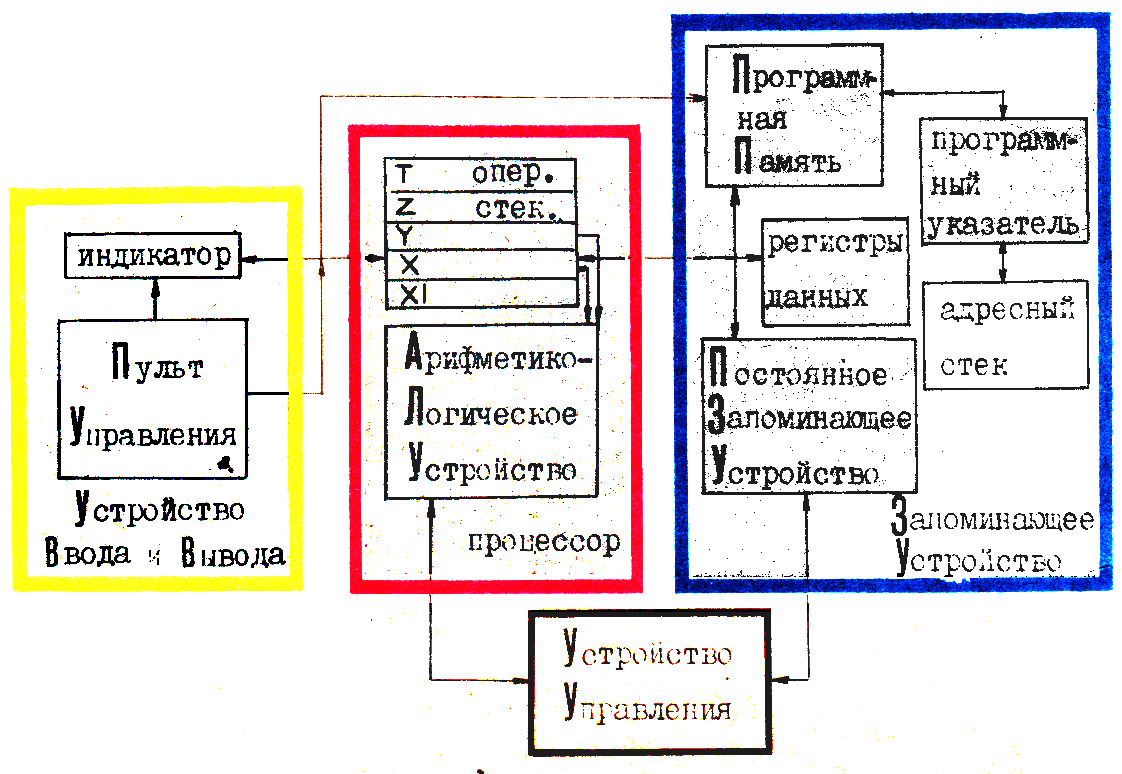
\includegraphics[width=\textwidth]{princip_scheme}

Принципиальная схема микрокалькулятора изображена на рисунке. Основными ее элементами являются устройство ввода и вывода информации (УВВ), устройство преобразования информации (процессор), запоминающее устройство (ЗУ) и устройство управления (УУ).

Устройство ввода и вывода — единственное, которое мы непосредственно видим. Состоит оно из клавиатуры, совмещающей функции устройства ввода и пульта управления, и индикатора. Программа и числа, вводимые с клавиатуры, отображаются на индикаторе. Туда же выводятся результаты вычислений. Индикатор, вообще говоря, — единственное "окно" в память машины, с помощью которого можно получить сведения о ее содержимом.

Команда, введенная с клавиатуры, попадает в запоминающее устройство. Состоит ЗУ из нескольких различных секций: программная память, регистры данных, постоянное запоминающее устройство (ПЗУ), а также программный указатель и адресный стек.

Программная память (ПП) представляет собой набор ячеек, в каждую из которых можно записать один код. Всего таких ячеек 98, нумеруются они двузначными числами  от 00 до 97. Количество ячеек определяет максимальную длину программы, которую можно ввести в память микрокалькулятору. Организована ПП наподобие "колеса обозрения". Адрес текущей ячейки записывается в программном указателе. При вводе команды адрес этот автоматически увеличивается на единицу и "колесо" поворачивается, подготавливая следующую "кабинку" (ячейку) для приема очередного "пассажира" (команды). Содержимое программного указателя можно изменять — с пульта или программным путем (об этом позже). При этом "колесо" может поворачиваться в любую сторону на заданное число позиций. Когда все 98 ячеек программной памяти заполнены, попытка ввести новую команду приводит к повороту "колеса" в начальное положение и команда попадает в первый адрес памяти, естественно стирая его старое содержимое.

Адресный стек состоит из пяти ячеек и используется для запоминания адреса команды, на которую нужно передать управление после окончания работы какой-либо подпрограммы (об использовании подпрограмм будет сказано в одной из следующих статей).

Регистры данных служат для записи и хранения числовой информации. Всего их 14. Таково максимальное количество чисел, которые можно одновременно хранить в памяти ПМК.

Постоянное запоминающее устройство содержит программы, которые, собственно, и организуют процесс вычислений. Эти программы нельзя изменить, они реализованы не программно, а аппаратно, то есть представляют собой совокупность электронных схем. Их нельзя даже прочесть, к ним можно лишь обращаться и получать результаты их работы. Именно программы из ПЗУ подсчитывают значения функций, названия которых записаны на клавиатуре, обеспечивают выполнение арифметических операций.

Выполняет же все операции по программам, хранящимся в ПЗУ, процессор — точнее, арифметическо- логическое устройство (АЛУ), работающее совместно с операционным стеком. В этом стеке 5 регистров: XI, X, Y, Z, Т. Числа движутся по регистрам либо автоматически (при выполнении некоторых операций), либо подчиняясь специальным командам. Подробно движение информации в стековых регистрах будет рассмотрено в одной из следующих статей. Особо важны два регистра: X и Y. Из них АЛУ черпает числовую информацию для выполнения двухместных операций: сложения, вычитания, умножения, деления и возведения в степень. Одноместные операции: извлечение квадратного корня, возведение в квадрат, вычисление тригонометрических функций и т. д. — производятся над содержимым регистра X.

В соответствии с кодом команды АЛУ вырабатывает результат операции и помещает его в регистр X. На экране отображается лишь содержимое этого регистра. Так что на индикаторе во время работы ПМК мелькают промежуточные результаты вычислений, появляющиеся в регистре X.

Наконец, устройство управления обеспечивает совместную работу всех блоков ПМК.

Зная функции отдельных элементов микрокалькулятора, проследим теперь полный цикл его работы при выполнении программы. Предположим, что она уже введена в память, установлен режим вычислений и все необходимые числа введены в нужные регистры. Нажимом клавиши «В/О» мы очищаем программный указатель, то есть устанавливаем его содержимое равным нулю. Клавиша, «С/П» запускает программу. Устройство управления считывает команду, адрес которой записан в программ ном указателе. После ее анализа и определения типа операции команда пересылается в АЛУ. По сигналам, поступившим из УУ, процессор вырабатывает результат операции. Затем УУ опрашивает программный указатель и выясняет, какая команда должна выполняться следующей. Потом цикл повторяется. Время выполнения цикла зависит от типа команды и колеблется от десятых долей секунды для команд типа записи и считывания, а также операций типа сложения, до нескольких секунд для вычисления тригонометрических функций. Знание времени выполнения отдельных команд помогает строить более быстродействующие программы.

Теперь подведем итоги.
\begin{enumerate}
\tightlist
\item Микрокалькулятор может работать в двух режимах: 1) ввода и редактирования программ и 2) вычислений. Первый устанавливается клавишами «F ПРГ», второй — «F АВТ». При включении ПМК автоматически устанавливается режим вычислений.
\item Программа для микрокалькулятора состоит из последовательности команд, вводится с клавиатуры и записывается в программную память. Помните, что адрес, который высвечивается при вводе в правом углу индикатора, — это адрес следующей вводимой команды.
\item Порядок работы с программой.
\begin{enumerate}[label=\arabic*)]
\item Установить режим «F ПРГ».
\item Ввести программу.
\item Перейти в режим вычислений «F АВТ».
\item Ввести постоянные в адресуемые регистры.
\item Установить начальный адрес считывания программы.
\item Набрать на клавиатуре значение переменного параметра.
\item Запустить программу на счет.
\item Если нужно повторить расчет для другого значения переменного параметра, перейти к пункту 6.
\end{enumerate}
\item Максимальная длина программы — 98 шагов, максимальное количество чисел, которые могут одновременно храниться в памяти, — 14.
\end{enumerate}

\subparagraph{двоичная система}
10 + 10 = 100!
Это не ошибка и не опечатка. Именно такой результат получается, если числа записаны в двоичной системе счисления.

Системой счисления называется способ выражения и записи чисел. Числа записываются в виде последовательности специальных символов. Смысл каждого символа зависит от позиции или разряда, в котором он записан. Количество единиц младшего разряда, объединяемого в одну единицу старшего, называется основанием системы, а символы, используемые для обозначения единиц каждого разряда, — цифрами.

Наиболее употребительна десятичная система. Мы настолько привыкли к этой системе, что "раскрываем" любое число не задумываясь. Например, $512 = 2 + 1 * 10 + 5*10^{2}$. Эта система представляется нам столь же естественной, как ребенку — родной язык. Но любая система счисления столь же естественна, как и любой язык. В вычислительной технике используются двоичная, восьмеричная и шестнадцатеричная система. Двоичная — самая простая и наиболее удобная для технической реализации. Цифр в ней всего две — 0 и 1. Когда в разряде (а называется двоичный разряд "бит"; несколько двоичных разрядов, чаще всего восемь, объединяются в "байт" — величину, с которой ЭВМ работает как с одним целым) накапливаются две единицы, то они заменяются единицей старшего разряда. Число $2_{10}$ (цифрой внизу обозначается основание системы) в двоичной системе записывается как $10_{2}$. Вообще любое число, записанное в n-ричной системе, переводится в десятичную очень просто. К последней n-ричной цифре прибавляется предпоследняя, умноженная на n, затем стоящая перед ней и умноженная на $n^{2}$, и т. д. Скажем, двоичное число $101_{2} = 1+0*2 + 1*2^{2} = 5_{10}$. Привлекательность двоичной системы, как уже говорилось, — в простоте технической реализации. Каждый разряд — это некоторое устройство, которое может находиться всего в двух состояниях.

В микрокалькуляторе для размещения одного символа кода отводится "тетрада" — четыре двоичных разряда. Легко подсчитать максимальное число, которое можно записать таким образом: $1111_{2} = 1 + 1 * 2 + 1 * 2^{2} + 1 * 2^{3} = 15_{10}$. Значит, коды должны изображаться числами в шестнадцатеричной системе. Так как десятичных знаков для изображения таких чисел не хватает, приходится "выдумывать" дополнительные символы. В ПМК число 10 изображается символом «—», 11 — «L», 12 — «С», 13 — «Г», 14 — «Е». "Цифра" 15 в обозначениях кодов не используется.

\section{Язык микрокалькулятора}
ИГОРЬ ДАНИЛОВ,
кандидат технических наук

Язык микрокалькулятора (как и любой язык) представляет собой набор символов, а также правил, определяющих, как с помощью этих символов писать и понимать написанное.

Правда, в отличие, скажем, от русского языка, где слова расчленяются на буквы, изменяются при склонении или спряжении, язык микрокалькулятора напоминает скорее китайский либо японский. Его "словарь" состоит из несклоняемых слов-иероглифов, и лишь порядком их следования определяется смысл текстов — программ для ПМК. Каждый из иероглифов — это имя команды: надпись на клавише или над ней (а в нижнем ряду — и под клавишей). Клавиши К и F самостоятельной роли не играют: по своему действию они подобны переключателю регистров пишущей машинки. Если требуется иероглиф, начертанный на клавише, то нужно нажать только ее, если же иероглиф, написанный над клавишей, то предварительно необходимо воспользоваться клавишей F (а в некоторых случаях — клавишей К). Каждая команда, независимо от количества нажимаемых клавиш (а оно для некоторых команд доходит до трех), отображается в памяти и на индикаторе одним двузначным шестнадцатеричным числом — кодом. Исключение составляют команды переходов: после них указывается адрес перехода, поэтому за кодом команды обязательно следует код этого адреса.

Полный набор команд «Электроники БЗ-34» приведен в таблице. Ею могут пользоваться и владельцы микрокалькуляторов «Электроника МК-54» и «Электроника МК-56» — система команд у них та же самая. Различаются лишь некоторые обозначения X→П вместо П, П→X вместо ИП, X←→У вместо \XY и В↑ вместо ↑, а также названия обратных тригонометрических функций — $sin^{-1}$, $cos^{-1}$, $tg^{-1}$ вместо arcsin, arccos, arctg. Смысл же операций и их коды полностью идентичные приведенным в таблице.

Условно всю совокупность команд можно разбить на два класса. К первому относятся команды, используемые в программе; ко второму — команды, предписывающие порядок работы ПМК. Последние вводятся в режиме вычислений; мы рассмотрим их при описании процесса отладки программ.

Первый класс можно подразделить на четыре группы: 1) вычислительные команды; 2) команды обмена информацией; 3) команды управления ходом вычислений; 4) команды, использующие режим косвенной адресации. Последние по своим функциям не отличаются от команд второй и третьей групп, но, поскольку используют иной режим адресации, будут рассмотрены отдельно. Особняком стоит команда К НОП.

К первой группе относятся прежде всего команды арифметических операций: сложение + (код 10), вычитание — (11), умножение X (12) и деление ÷(13). Все они двухместные — работают с содержимым двух регистров стека X и Y, причем при вычитании в X записывается вычитаемое, а при делении — делитель. Результат каждой из арифметических операций заносится в регистр X, прежнее содержимое этого регистра перемещается в XI. То, что было в Y, пропадает, замещаясь числом из регистра Z, а в Z заносится содержимое регистра Т. Но при этом прежнее содержимое регистра Т остается и на своем месте.

Надо сказать, что микрокалькулятор способен работать не со всякими числами. Максимальное не должно превосходить $10^{100}$ (точнее, $9,9999999*10^{99}$), минимальное должно быть не меньше $10^{99}$ — в противном случае вместо нормального восьмиразрядного числа в память и на индикатор запишется "чистый" нуль. Наибольшую осторожность надо соблюдать при умножениях и делениях. Иногда случается, что конечный результат цепочки операций лежит в пределах возможностей ПМК, а на промежуточном этапе возникает аварийная остановка. Её можно избежать, правильно организуя процесс вычислений.

Рассмотрим простой пример. Нужно вычислить значение дроби $a*b/c$, где $а=2*10^{51}$, $b=3*10^{49}$, $с=4*10^{50}$. Легко видеть, что результат ($1,5*10^{50}$) лежит в допустимых пределах. Но если соответствующий фрагмент программы записать так: ИП А, ИП В, X, ИП С, ÷, то есть сначала выполнять умножение (мы считаем, что исходные величины хранятся в одноименных регистрах), то после первого же действия получается число $6*10^{100}$, возникает "аварийный" останов, на экране появляется сообщение ЕГГО.Г и вычисления прекращаются. Если же выполнять сначала деление (например, записать тот же фрагмент так: ИП А, ИП С, ÷, ИП В, X)» то никаких неприятностей не произойдет.

К арифметическим можно отнести и команду (—) (код 0L). Она одноместная, использует только регистр X. При ее выполнении меняется знак числа, находящегося в этом регистре (плюс на минус или наоборот).

Остальные вычислительные команды используются для расчета значений различных функций. Их названия написаны над соответствующими клавишами. Чтобы получить значение какой-либо из них, нужно предварительно нажать клавишу F, но для краткости при описании команд мы ее упоминать не будем.

Какие же функции доступны нашему ПМК? Вот они: извлечение квадратного корня $\sqrt{}$ (код 21);
возведение в квадрат $X^{2}$ (22); получение обратной величины $1/X$ (23); возведение числа 10 в любую степень $10^{x}$ (15) и возведение в степень числа е, основания натуральных логарифмов $e^{x}$ (16); вычисление десятичного и натурального логарифмов lg (17) и ln (18); вычисление тригонометрических функций (аргументы могут быть заданы как в градусах, так и в радианах) sin (1C), cos (1Г), tg (1E), а также обратных тригонометрических функций arcsin (19), arccos (1—) и arctg (1L). Аргумент для каждой из этих функций берется из регистра X, туда же записывается результат, а аргумент после выполнения операции перемещается в XI. Содержимое других регистров не меняется.

Особняком среди команд подобного рода стоит $Х^{y}$ (24) — возведение произвольного числа в любую степень. Возводимое число берется из регистра X, а показатель степени — из Y. После выполнения команды результат, как и обычно, заносится в X, то, что было там прежде, переходит в XI, а вот содержимое Y, как и остальных регистров, остается на месте. Отметим, что эту команду «Электроника БЗ-34» выполняет хуже других: результата приходится ждать долго, да и точность его ниже, чем при выполнении других команд. Так, $2^{2}$, вычисленное по этой команде, "равно" 3,9999996. А вот если использовать команду $X^{2}$, результат равен в точности четырем. Калькуляторы же первых выпусков при выполнении команды $X^{y}$ иногда вообще ошибаются. Так что рекомендуем по возможности ее избегать.

Вычислительные команды способны работать не со всеми возможными числами. Иногда это ограничения чисто математические (нельзя, скажем, извлекать квадратный корень из отрицательного числа или вычислять его логарифм), иногда диктуются возможностями ПМК. Поскольку числа, доступные микрокалькулятору, ограничены по абсолютной величине, то аргументы функций $10^{x}$ и $e^{x}$ не могут превосходить соответственно 99,999999 и 230,25. Не допускаются и отрицательные аргументы, по абсолютной величине превосходящие эти числа. Функция $X^{y}$, независимо от величины показателя, не определена для отрицательных оснований. При вычислении тригонометрических функций запрещается выбирать в качестве аргумента числа, превышающие $10^{1}$ (независимо от того, измеряются ли они в градусах или в радианах).

Напомним, что в микрокалькуляторах типа «Электроника БЗ-34» используется обратная бесскобочная (или польская) запись арифметических выражений. Сначала выписываются аргументы операции, а потом ее символ — например, не аХb, а аbХ; не $\sqrt{c}$, а $c\sqrt{}$.

При составлении программ нужно следить, чтобы перед совершением каждой арифметической операции стек был заполнен так, как требуется для ее выполнения.

\begin{figure}[H]
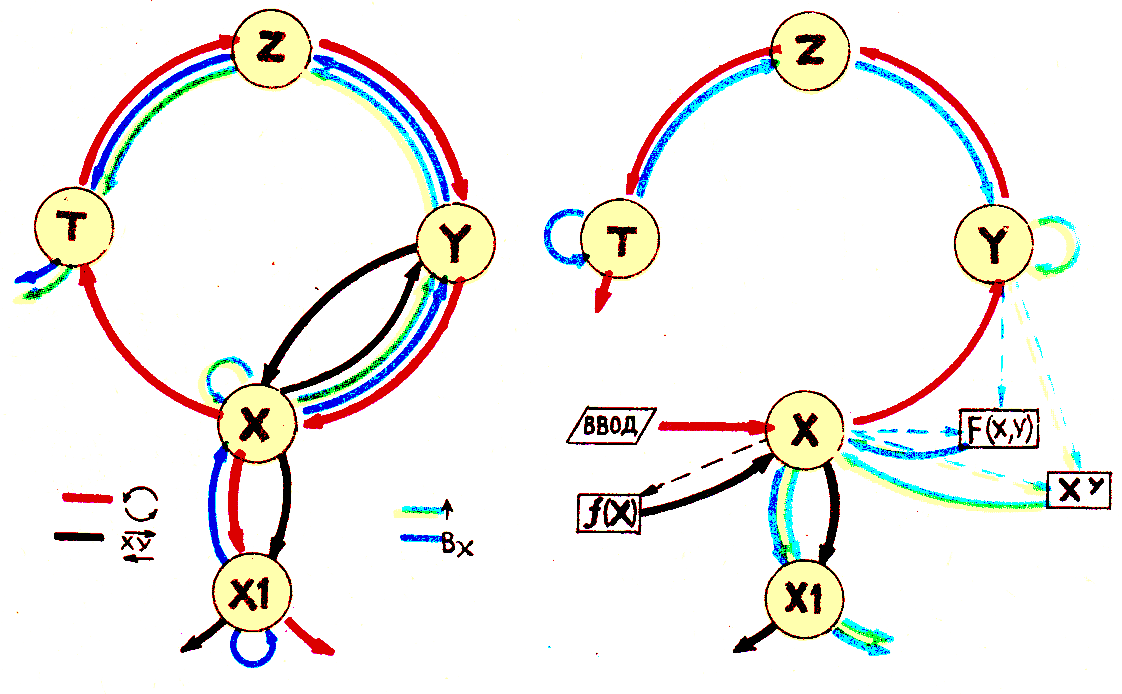
\includegraphics[width=\textwidth]{stack}
\caption{Движение информации по регистрам стена при выполнении команд обмена информацией (слева), ввода и вычислительных операции (справа).}
\end{figure}

Перемещением чисел по регистрам стека и по регистрам данных "заведуют" команды второй группы (команды обмена информацией). Это ↑(0Е), FВх (0), \XY (14) и \FO (25). Первая из них, ↑ используется чаще всего для разделения вводимых чисел. Она сдвигает числа в стеке "снизу вверх" (см. рис.), сохраняя содержимое регистра X и выбрасывая за пределы стека число, хранившееся в регистре Т. FBx используется для вызова содержимого регистра предыдущего результата (XI) в регистр X. В остальном ее действие подобно действию предыдущей команды; сдвиг чисел в стеке "снизу вверх" и вытеснение содержимого регистра Т. Команда \XY меняет местами содержимое регистров X и Y; при этом число, находившееся в регистре X, дополнительно копируется и в регистре XI, вытесняя его прежнее содержимое. То, что было в остальных регистрах, при этом не меняется. \FO совершает круговой обмен: число из регистра X перемещается в Т, содержимое Y передвигается в X, Z — в Y, а Т — в Z. Пропадает при этом только содержимое регистра XI: туда копируется число из X. Движение информации при выполнении всех этих команд отражено на диаграммах.

Есть 14 команд, позволяющих пересылать содержимое регистра X в адресуемые регистры (или регистры данных). Всего их тоже 14. Первые десять обозначаются цифрами от 0 до 9, последние — буквами А, В, С, Д. Для занесения в них информации служат команды: ПО (код 40), П1 (41)... П9 (49). ПА (4—), ПВ (4L), ПС (4С) и ПД (4Г). Каждая из команд требует набора двух клавиш: П и номера регистра (цифры или буквы), но, как мы видим, отображаются они одним кодом — как в памяти, так и на индикаторе. Обратите внимание, что буквы А, В, С и Д написаны под клавишами, но после нажатия клавиши П воспринимаются именно они.

Для вызова информации из адресуемых регистров в регистр X служат команды ИП0 (код 60)... ИП9 (69), ИПА (6—)... ИПД (6Г). Условно к ним можно отнести и команду Fπ, действие которой заключается в вызове записанного в ПЗУ числа π в регистр X.

В языке микрокалькулятора нет специальных команд ввода. Числа просто набираются на клавиатуре и автоматически заносятся в регистр X. Однако можно хранить числа и в программной памяти. Например, если нужно умножить содержимое регистра 0 на 2, мы пишем обычно: ИП0, 2, X. Теперь при работе программы число 2 вводить не надо — оно занесено в программную память, занимая в ней одну ячейку. Для многозначных чисел такая запись, как правило, нецелесообразна. Например, если мы решим занести в программную память вместо двойки число 2,58, то соответствующий фрагмент программы будет выглядеть так: ИП0, 2, «,», 5, 8, X. Одно число занимает целых четыре ячейки — слишком много! Однако если все адресуемые регистры заняты, а в ПП место есть, то волей-неволей приходится прибегать и к этому способу. Коды цифр совпадают с ними самими (от 00 до 09); кроме них, при вводе чисел в ПП используются символы «,» (код 0—) и ВП (ОС) — ввод порядка. Так, для записи в ПП числа $1,6*10^{-19}$ (заряд электрона в кулонах) нужно ввести команды: 1, «,», 6, ВП, 1, 9, /—/.

Последняя команда этой группы — Сх (код 0Г). Она "стирает" содержимое регистра X (вернее, засылает туда число 0).

Рассмотренных команд достаточно для написания несложных программ, производящих вычисления по последовательным формулам. Однако для многих задач этого набора недостаточно. Даже при решении элементарного квадратного уравнения требуется сначала проверить знак дискриминанта квадратного трехчлена, чтобы знать, вычислять ли действительные корни уравнения, или же действительную и мнимую части корней комплексных. То есть нужно сначала выбрать путь и лишь потом начинать вычисления.

В языке микрокалькулятора имеются средства для проведения подобных операций. Это команды управления программой.

Наиболее часто употребляется команда останова С/П (код 50). Она используется для приостановки процесса вычислений, когда нужно либо прочесть полученный результат, либо ввести с клавиатуры какие-нибудь числа или предписывающие команды. В каждой программе обязательно есть хотя бы одна команда С/П — не может же программа работать бесконечно!

Команда безусловного перехода БП (51) передает управление команде, адрес которой записан сразу после нее. Фактически она занимает в памяти две смежные ячейки: в первой записан код 51, во второй — другое двузначное число, адрес перехода. Так что две цифры подряд,набранные после команды БП, записываются одним кодом — числом от 00 до 97 (напомним, что память ПМК состоит из 98 ячеек, поэтому адресов 98 и 99 попросту нет).

Команды условного перехода тоже передают управление, но лишь при выполнении определенных условий. В качестве условия в этих командах нашего ПМК используется сравнение содержимого регистра X с нулем. Если условие, записанное в команде, выполнено, то управление передается на следующую по порядку команду, в противном случае — по указанному адресу. Например, условный переход х<0, 23 выполняется так. Если число, находящееся в регистре X, меньше нуля, то выполняется команда, следующая за приведенным фрагментом, в противном случае — команда, код которой записан по адресу 23. Команд условного перехода четыре: х<0 (5С), х=0 (5Е), х≠0 (57), х⩾0(59).
Поскольку названия их написаны над клавишами, то перед ними нужно нажимать клавишу F.

Есть среди команд перехода четыре команды, предназначенные для организации циклов — многократного выполнения заданной последовательности команд. Это L0 (код 5Г), L1 (5L), L2 (58) и L3 (5—). Перед каждой из них тоже, естественно, нажимается клавиша F. А после каждой указывается адрес перехода. При обращении к одной из команд организации цикла из содержимого соответствующего (имеющего тот же номер) регистра данных вычитается единица, и, если результат не равен нулю, управление передается по указанному адресу перехода. Если же результат равен нулю, цикл завершается, и выполняется команда, записанная после адреса перехода. Таким образом, заслав в один из первых четырех регистров данных некоторое число n, мы получаем возможность выполнить некоторую часть программы n раз.

Последняя из программ перехода — это ПП (код 53) — переход на подпрограмму. Структура ее такая же, как и у остальных: сначала записывается сама команда, за ней — адрес перехода. Но в отличие от команды БП она не только "безусловно" передает управление по заданному адресу, но и после отработки подпрограммы — а последнюю обязательно завершает команда В/О (возврат/очистка, код 52), — автоматически возвращает программу "на старое место" — к команде, следующей за ПП.

Особняком стоит команда К НОП (код 54), которая набирается двумя клавишами К и НОП. Это — "пустая" команда, она не совершает никаких действий. Употребляется обычно при отладке программ: если выяснится, что одна из команд лишняя, то, чтобы не переписывать остальные, на ее место записывают "пустую" команду.

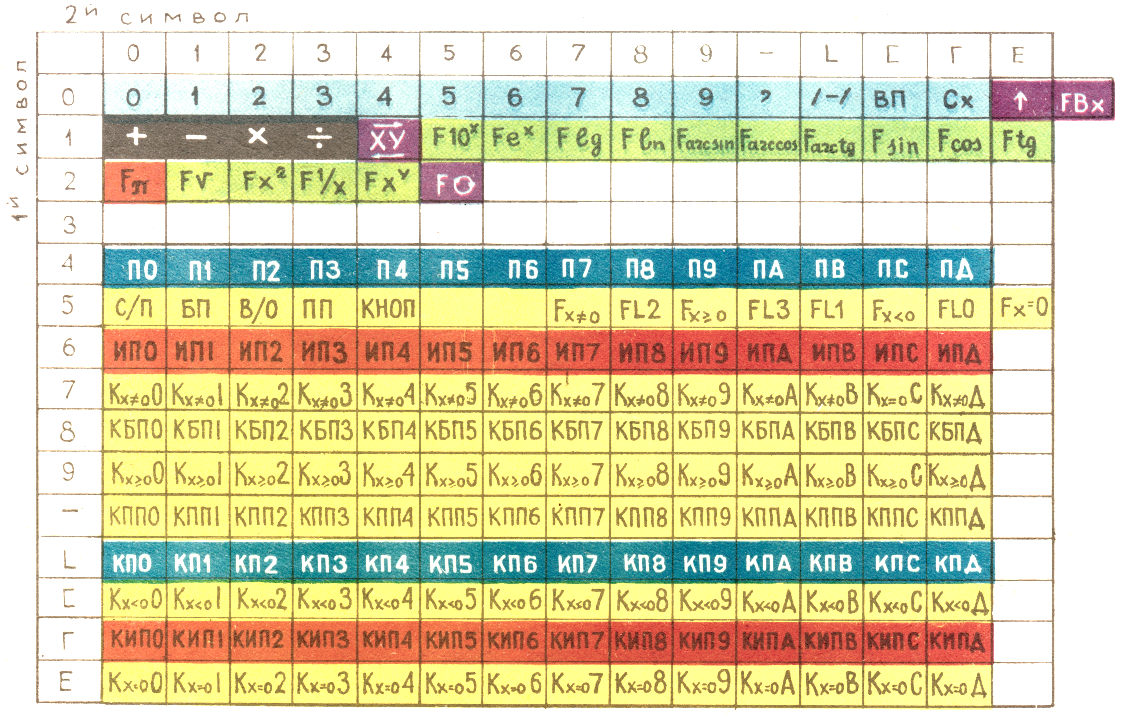
\includegraphics[width=\textwidth]{commands}

Команды косвенной адресации мы рассмотрим позже. Подведем краткие итоги.

\begin{enumerate}
\item Язык микрокалькулятора — это набор команд, имена которых написаны на клавиатуре. Чтобы использовать команды, названия которых даны над клавишами, нужно предварительно нажать клавишу F. Перед командой НОП нужно нажать клавишу К.
\item Каждая вычислительная команда размещается в одной ячейке памяти.
\item Результаты работы вычислительных команд помещаются в регистр X. Исходные данные для одноместных операций черпаются из этого же регистра, а для двухместных — из регистров X и Y.
\item Во всех операциях по записи информации в регистры данных и по ее извлечению обязательно участвует регистр X. В регистры данных можно засылать только его содержимое, и только в него можно считывать числа из этих регистров.
\item Команды перехода записываются в двух смежных ячейках памяти (в первой — сама команда, во второй — адрес перехода). Адрес перехода обязательно набирается в виде двузначного, числа.
\item При использовании вычислительных команд нужно следить за тем, верно ли расположены в регистрах, стека аргументы операций, и, кроме того, помнить об ограничениях, накладываемых на величину аргументов. Если последняя выходит за пределы допустимых ограничений, работа программы прекращается и на индикатор выводится сообщение ЕГГОГ.
\item Старайтесь по возможности избегать употребления команды $X^{y}$. Работает она медленно, а ошибки при вычислениях дает большие.
\end{enumerate}

\section{Блок-схема - портрет программы}

ИГОРЬ ДАНИЛОВ, кандидат технических наук

Что необходимо для составления программы? На вопрос этот можно ответить в двух словах, только для непосвященного каждое из них требует особого пояснения.

Первое из этих слов — алгоритм, то есть точное предписание, определяющее процесс переработки исходных данных в искомый результат.

Рассмотрим конкретный пример. Как известно, корни квадратного уравнения $ax^{2}+bx+c=0$ вычисляются по формулам:

\begin{equation}
X_{1}=\frac{-b+\sqrt{b^{2}-4ac}}{2a}
\end{equation}

\begin{equation}
X_{2}=\frac{-b-\sqrt{b^{2}-4ac}}{2a}
\end{equation}

Где здесь исходные данные? Набор коэффициентов a, b, c. Чем определяется искомый результат? Двумя приведенными формулами. В чем заключается процесс переработки исходных данных? В вычислениях по этим формулам.

Читатель, научившийся приводить расчетные формулы к "машинному" виду, легко сделает это и на сей раз:

\begin{equation}
B=\frac{b}{2} ; d=\sqrt{B^{2}-ac}
\end{equation}

\begin{equation}
X_{1}=\frac{-B+d}{a}; X_{2}=\frac{-B-d}{a}
\end{equation}

Эта последовательность формул и будет уточненным алгоритмом.

Второе слово — блок-схема. Так программисты называют своеобразный "графический портрет" алгоритма, согласно которому будет решаться задача. Блок-схема является незаменимым подспорьем при разработке программы. Даже опытные программисты, как правило, начинают работу над программой с наброска блок-схемы. При дальнейшей детализации она уточняется настолько, что перевод ее на язык команд почти не требует напряжения мысли.

Чтобы нарисовать блок-схему, особых дарований не требуется. Для обозначения блоков, составных элементов блок-схемы, достаточно четырех фигур: это круг, прямоугольник, параллелограмм и ромб. В верхней части блок-схемы находится кружок с надписью "Начало", в нижней — со словом "Конец". Все остальные блоки располагаются между этими двумя.

\includegraphics[width=0.3\textwidth]{algo1}

Параллелограммы со словами «Ввод» и «Вывод» указывают, в каких местах программы нужно вводить исходные данные или выводить на индикатор результаты вычислений. Сами же вычисления — формулами либо словами — описываются в прямоугольниках. Последовательно нарисованные прямоугольники можно объединять. К примеру, в нашей блок-схеме вычисления по всем формулам можно описать единым блоком (намечено пунктиром).

Линии, соединяющие блоки, показывают последовательность обработки данных. «Положительными» считаются направления вниз и вправо. Если информация движется по этим направлениям, стрелки на линиях можно не ставить. В иных случаях стрелки обязательны.

Наша блок-схема проста, но «работает» она не при всех значениях а, b, с. Что будет, например, если а=0? Уравнение при этом отнюдь не усложняется — наоборот, превращается в более простое, линейное, с
единственным корнем x=-c/b. Человек-вычислитель реагирует на подобные обстоятельства автоматически:	в его памяти есть для этого необходимая информация. А в памяти машины имеется лишь то, что туда заложит человек — разработчик или программист. Разработчики ПМК вложили в него предостережение: делить на ноль нельзя. А в наших формулах для корней квадратного уравнения есть деление на а. На а, которое равно нулю. И машина не сможет справиться с задачей, хотя та и стала проще. Произойдет аварийный останов, и на индикаторе загорится: ЕГГОГ.

Значит, нужно научить нашего электронного помощника, как поступать в столь каверзных ситуациях! Иначе говоря, предусмотреть в алгоритме все мыслимые варианты исходных данных.

Ясно, что раз при a=0 расчеты следует производить по другим формулам, значит, нужно вставить в программу блок, где машина бы проверяла коэффициент а на равенство нулю и в зависимости от результатов проверки выбирала путь решения. Может далее статься, что и a=0 и b=0. Тогда из уравнения выпадает неизвестная величина х, и решать его вообще не имеет смысла. Нужно научить машину реагировать и на такое сочетание коэффициентов.

Да и выполнения неравенства а≠0 еще недостаточно, чтобы без опаски вести расчеты по выписанным формулам. Ведь если дискриминант уравнения отрицателен, то оно имеет два комплексных корня: нужно вычислять отдельно действительные части (они у обоих корней одинаковы) и мнимые (они отличаются только знаком).

Итак, сравнение коэффициента а с нулем разветвляет нашу блок-схему надвое, и каждая из ветвей также разделяется на два направления. На каждой «развилке», подобно стрелке на железнодорожных путях, ставится блок сравнения. Он изображается ромбом, внутри которого записана операция сравнения. Выходят из ромба две линии, два возможных пути. Один помечен словом «Да» (сюда надо свернуть, если условие выполняется), другой — словом «Нет» (если не выполняется). Чтобы не перегружать блок-схему, мы не стали анализировать практически бессмысленную ситуацию, когда все три коэффициента равны нулю; в этом случае уравнению удовлетворяют любые х.

Как видим, исчерпывающий анализ даже привычного квадратного уравнения — дело довольно сложное. Зато достоинства представления алгоритма в виде блок-схемы налицо. Предписания, записанные в ее элементах, понятны и просты, они избавляют составителя программы от необходимости хранить в своей собственной памяти излишнюю информацию.

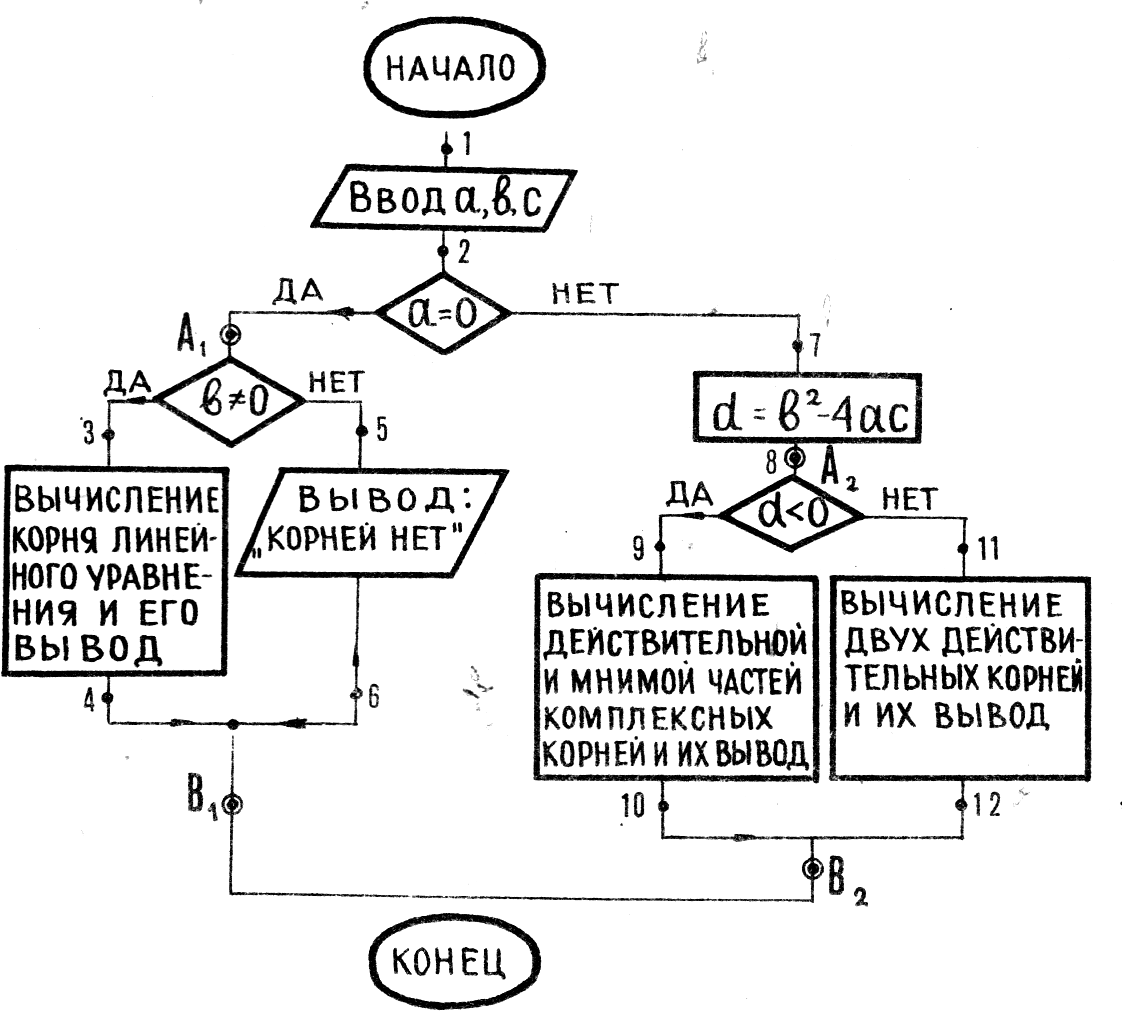
\includegraphics[width=0.5\textwidth]{sqroot_algo1}
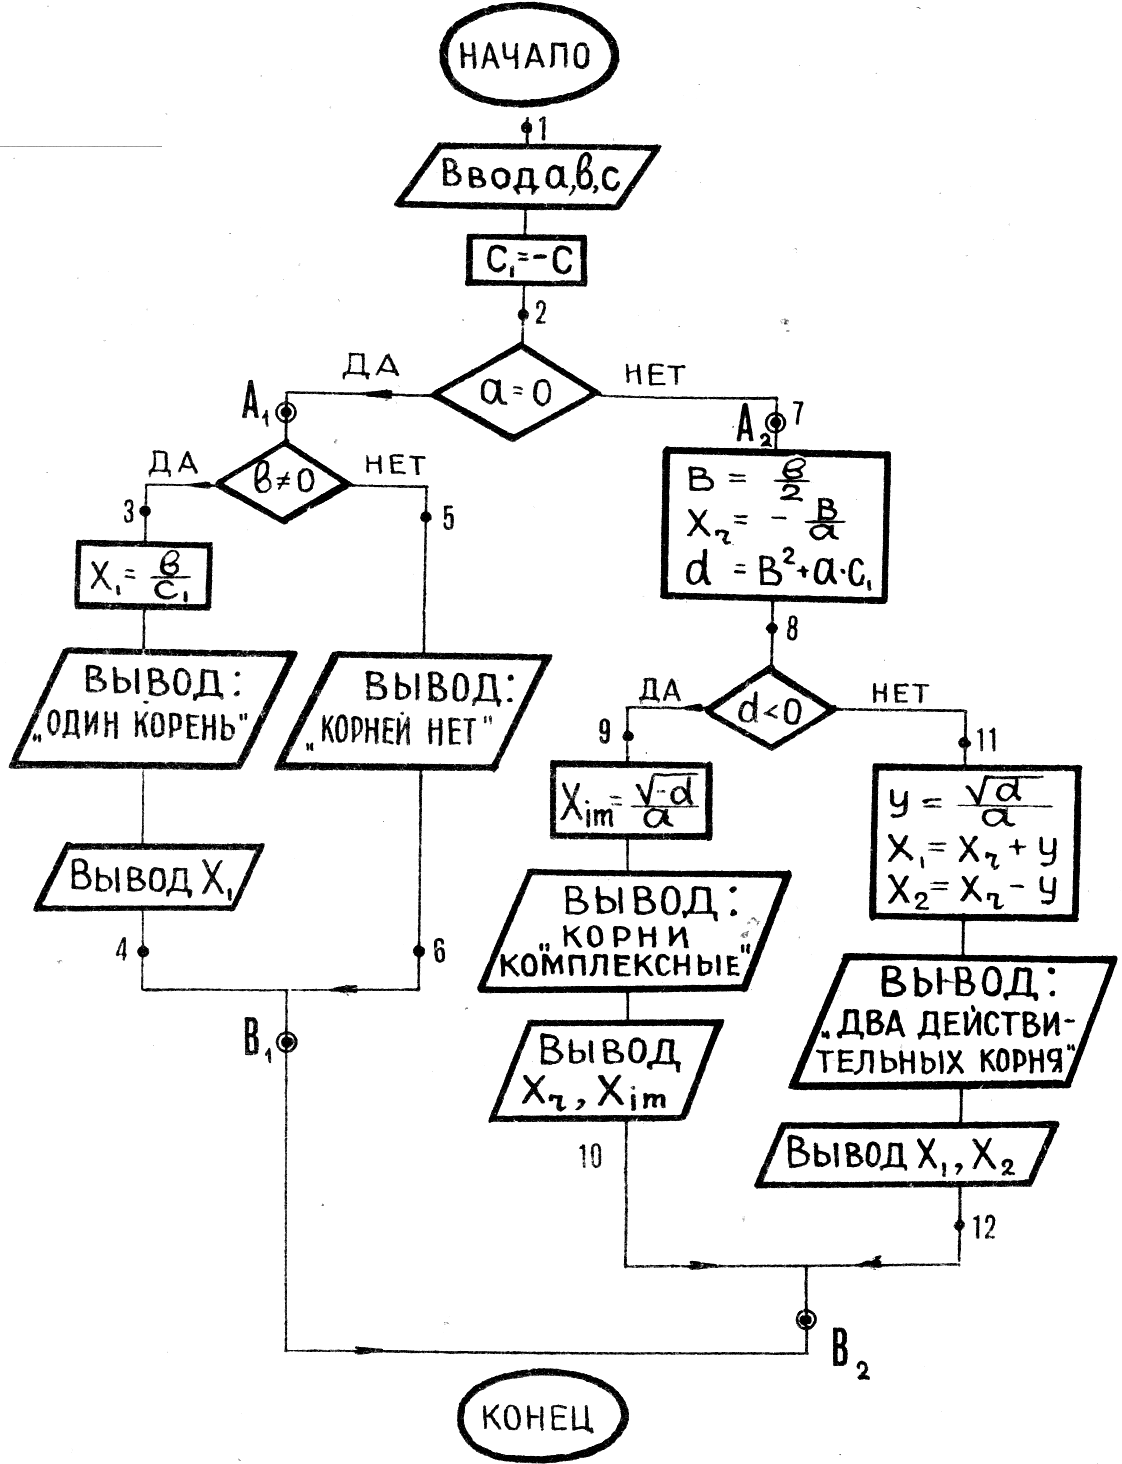
\includegraphics[width=0.5\textwidth]{sqroot_algo2}

Прежде чем приступить к написанию программы по блок-схеме, последнюю нужно детализировать, заменив словесные описания последовательностью формул. Чтобы различать отдельные части блок-схемы, мы пометили некоторые ее узлы цифрами. Детализация той ветви, что лежит между узлами 11 и 12, уже проведена: сюда надо просто вставить формулы из первого варианта блок-схемы. Для ветви 5-6 никаких формул не надо — вся работа на этом этапе заключается в выводе сообщения: «Корней нет». Остались две ветви. Для одной из них, 3-4, требуется всего одна формула:

\begin{equation}
x_{1}=-\frac{c}{b}
\end{equation}

А вот формулы для последней ветви 9-10:

\begin{equation}
B=\frac{b}{2}; d=\sqrt{B^{2}-ac};
\end{equation}
\begin{equation}
x_{r}=-\frac{B}{a}; x_{im}=\frac{d}{a}
\end{equation}

Здесь $x_{r}$ и $x_{im}$ — действительная и мнимая части комплексных корней, которые с помощью так называемой мнимой единицы, величины $i=\sqrt{-1}$, выражаются формулами:
$x_{1}=x_{r} + ix_{im}; x_{2} = x_{r} — ix_{im}$ Легко видеть, что в формулах для ветвей 9-10 и 11-12 много общего. Это означает, что одни и те же последовательности команд будут написаны дважды. Можно ли обойтись без такого дублирования? Да. Целесообразно выполнять общие для каких-то ветвей вычисления еще до разделения ветвей. Заметим также, что во всех формулах коэффициент с используется со знаком минус. Казалось бы, все равно, какую операцию использовать — сложение или вычитание. Но здесь надо учитывать специфику микрокалькулятора. Перед вычитанием пришлось бы правильно расставить по регистрам стека вычитаемое и уменьшаемое: первое — в X, второе - в Y. При сложении расстановка слагаемых значения не имеет, поэтому сложение предпочтительнее. Целесообразно заблаговременно сменить знак коэффициента, лучше всего сразу после его ввода. Все эти соображения учтены в новом варианте блок-схемы.

Вот теперь можно уже писать программу. Отметим, что наша блок-схема пригодится при составлении программы для любой ЭВМ и на любом языке программирования. Она подобна записи мелодии, которую затем можно аранжировать для любого инструмента с учетом его специфики...

Специфика микрокалькулятора проявляется, в частности, в двух моментах. Во-первых, у него разделены области памяти для хранения программ и данных. Во-вторых, ПМК оперирует только цифрами — буквенных символов в его языке нет. В силу первой особенности приходится вручную распределять информацию по регистрам, а вторая заставляет шифровать цифрами сообщения об особенностях решения (в нашем случае — о количестве и природе корней).

С распределением переменных по регистрам справляемся без труда. Предварительно намечаем такой вариант:

$a \rightarrow A; b \rightarrow B; c (c1 = -c) \rightarrow C;
x_{1} (x_{r}) \rightarrow 1(X); x_{2}(x_{im}) \rightarrow 2(Y)$.

Почему этот вариант предварительный? Да потому, что в процессе составления программы могут понадобиться дополнительные регистры или, наоборот, какие-либо из запланированных окажутся лишними.
Придумать систему шифров для необходимых сообщений тоже нетрудно. Скажем, появление на индикаторе нуля означает: «Корней нет», появление единицы — «Имеется один корень» и т. д. Часто так и поступают. Однако у этого метода есть существенный недостаток: можно спутать шифрованное сообщение с результатом вычислений. К счастью, есть и другой путь.

Мы уже знаем, что в микрокалькуляторе используются и такие символы для записи шестнадцатиричных чисел, которые не спутаешь ни с одной десятичной цифрой. Оказывается, есть возможность, формально выполняя некоторые «противозаконные» операции, получать на индикаторе и запоминать в адресуемых регистрах комбинации этих символов с обычными цифровыми. Их-то и удобно использовать в качестве сообщений; как их получать, скажем позже, а пока договоримся использовать следующие шифры: Е00	— «Корней нет», Е01 — «Один корень», Е02 — «Два действительных корня» и Г. — «Корни комплексные». Для хранения шифров тоже нужны регистры. Поэтому в дополнение к предварительному распределению памяти запишем: Е00→0, Е02→4, Е01→3, Г.→5. (Цифрами 0, 3, 4, 5, как и раньше, обозначены номера адресуемых регистров.)

Далее нужно продумать организацию ввода и вывода информации. Можно, конечно, вводить значения коэффициентов сразу в соответствующие адресуемые регистры в режиме вычислений, а результаты читать, вызывая на индикатор содержимое нужных регистров после останова, Однако большое число требуемых для этого ручных операций и необходимость постоянно помнить, что куда вводить и что откуда выводить, резко увеличат общее время получения результата, да и возможность ошибок возрастет. Лучше организовать ввод и вывод так, чтобы введенные числа автоматически рассылались по нужным регистрам и чтобы для прочтения результатов приходилось бы нажимать как можно меньше клавиш.

Остановимся на такой структуре ввода-вывода: коэффициенты вводятся в естественной последовательности — a, b, c; окончанием каждого ввода является нажатие клавиши С/П; после останова на индикаторе появляется шифрованное сообщение о характере результата, затем, после нажима С/П и следующего останова, высвечивается один корень, а после нажима клавиши \XY — второй (если он есть),

Все технические требования к программе изложены, можно приступать непосредственно к ее составлению. Рекомендуем записывать программу так, как показано на рисунке, — указывать, кроме самих команд, их адресов и кодов, еще и содержимое регистров стека, хотя бы тех, которые могут понадобиться в дальнейшем. Желательно оставить еще одну колонку для кратких примечаний. Они помогут ориентироваться в программе — иной раз легче написать новую, чем разобраться в старой. Мы же в первом примере используем подробные примечания.

\begin{table}[H]
\begin{tabular}{|l|l|l|l|l|l|l|l|l|l|l|l|l|l|l|l|}
\rotatebox{90}{АДРЕС} & \rotatebox{90}{КОМАНДА} & \rotatebox{90}{код} & стек   &     &     &   &    & \rotatebox{90}{АДРЕС} & \rotatebox{90}{команда}& \rotatebox{90}{код} & стек    &     &    &   &        \\
      &         &     & X      & У   & z   & т & XI &       &     &     & X           & y   & Z  & т & X1     \\
00    & ПА      & 4-  & a      &     &     &   &    & 31    & ИПА & 6-  & а    & B   & d  &   &        \\
01    & с/п     & 50  & b      & а   &     &   &    & 32    & ÷   & 13  & B/a  & d   & а  &   &        \\
02    & ↑       & 0Е  & b      & b   & а   &   &    & 33    & /-/ & 0L  & $x_{r}$& d   & а  &   &        \\
03    & с/п     & 50  & c      & b   & а   &   &    & 34    & П1  & 41  & $x_{r}$& d   & а  &   &        \\
04    & /-/     & 0L  & $-c=c_{1}$& b  & а   &   &  & 35    & \XY  & 14  & d    & $x_{r}$&    &   &        \\
05    & ИПА     & 6-  & а      &$ c_{1}$& b   &   & & 36    & Fx\textless{}0 & 5C  &      &     &    &   &        \\
06    & Fx=0    & 5Е  &        &     &     &   &    & 37    & 48  & 48  &      &     &    &   &        \\
07    & 23      & 23  &        &     &     &   &    & 38    & /-/ & 0L  & -d   & $x_{r}$& а  &   &        \\
08    & \FO      & 25  & $c_{1}$  & b   & а   &   & & 39    & F√  & 21  & $\sqrt{-d}$  & $x_{r}$  & а  &   & \\
09    & XY      & 14  & b      & $c_{1}$&     &   & & 40    & ИПА & 6-  & а    & $\sqrt{-d}$ & $x_{r}$ &   &        \\
10    & Fx≠o    & 57  &        &     &     &   &    & 41    & ÷   & 13  & $(\sqrt{-d})/a$ & $x_{r}$  &    &   & \\
11    & 19      & 19  &        &     &     &   &    & 42    & ИП5 & 65  & Г.   & $x_{im}$ & $x_{r}$ &   &        \\
12    & ÷       & 13  & $c_{1}/b$ &     &     &   & & 43    & с/п & 50  &      &     &    &   &        \\
13    & ИП3     & 63  & Е01    & $x_{1}$&     &   & & 44    & \FO  & 25  & $x_{im}$  & $x_{r}$  &    &   &        \\
14    & с/п     & 50  &        &     &     &   &    & 45    & с/п & 50  &      &     &    &   &        \\
15    & \XY      & 14  & $x_{1}$  & E01 &     &   & & 46    & БП  & 51  &      &     &    &   &        \\
16    & с/п     & 50  &        &     &     &   &    & 47    & 59  & 59  &      &     &    &   &        \\
17    & БП      & 51  &        &     &     &   &    & 48    & F√  & 21  & $\sqrt{d}$   & $x_{r}$  & а  &   &        \\
18    & 59      & 59  &        &     &     &   &    & 49    & ИПА & 6-  & а    & $\sqrt{d}$  & $x_{r}$ &   &        \\
19    & ИП0     & 60  & Е00    & b   &     &   &    & 50    & ÷   & 13  & $(\sqrt{d})/a$  & $x_{r}$  &    &   &        \\
20    & с/п     & 50  &        &     &     &   &    & 51    & +   & 10  & $x_{r}+(\sqrt{d})/a$  &     &    &   &        \\
21    & БП      & 51  &        &     &     &   &    & 52    & ИП1 & 61  & $x_{r}$   & $x_{1}$  &    &   & $(\sqrt{d})/a$ \\
22    & 59      & 59  &        &     &     &   &    & 53    & FBx & 0   & $(\sqrt{d})/a$  & $x_{r}$  & $x_{1}$ &   &        \\
23    & X       & 12  & $ac_{1}$ & b   & а   &   &  & 54    & -   & 11  & $x_{r}-(\sqrt{d})/a$ &     &    &   &        \\
24    & \XY      & 14  & b      & $ac_{1}$& а   &   & 55    & ИП4 & 64  & Е02  & $x_{2}$  & $x_{1}$ &   &        \\
25    & 2       & 02  & 2      & b   & $ac_{1}$& а && 56    & с/п & 50  &      &     &    &   &        \\
26    & ÷       & 13  & $b/2=B$  & $ac_{1}$ & а & & & 57    & \FO & 25  & $x_{2}$   & $x_{1}$  &    &   &        \\
27    & ПВ      & 4L  & B      & $ac_{1}$ & а   & & & 58    & с/п & 50  &      &     &    &   &        \\
28    & $Fx^{2}$  & 22 & $B^{2}$ & $ac_{1}$ & а & & & 59    & БП  & 51  &      &     &    &   &        \\
29    & +       & 10  & $B^{2}+ac_{1}$ & а   &&  &  & 60    & 00  & 00  &      &     &    &   &        \\
30    & ИПВ     & 6L  & B      & d   & а   &   &    &       &     &     &      &     &    &   &       
\end{tabular}
\end{table}

«Ввод а». Эта операция выполняется перед пуском программы. Величина а набирается на клавиатуре. Набор заканчивается нажимом клавиши С/П.

00. Запись а в адресуемый регистр А.

01. Останов для ввода b. Набираем значение коэффициента на клавиатуре и снова нажимаем С/П.

02. Подготовка стека для приема значения с.

03. Введен третий параметр уравнения, коэффициент с. Ввод закончен. Теперь клавиша С/П запускает программу на счет.

04. Вычисляем $c_{1} =-c$. (Внимание: задавать с в экспоненциальном виде нельзя; в этом случае команда 04 изменит знак не мантиссы, а показателя.)

05. Проще всего вызвать а из «собственного» регистра А.

06-07. В стеке ничего не меняется. Мы лишь проверили, равно ли нулю содержимое регистра X. Если да, то есть если уравнение вырожденное, будем выполнять команду по адресу 08 (ветвь A1-В1. Если нет — перейдем к команде, записанной по адресу 23 (ветвь А2-В2).

08-09. Две команды использованы только для того, чтобы вернуть в регистр X значение b. Казалось бы, можно обойтись и одной — ИП В. Но нужно «помнить о будущем» — скоро придется делить $c_{1}$ на b, а при таком распределении чисел в стеке, как теперь, для этого все подготовлено.

10-11. Если b = 0, то перейдем к команде по адресу 19 (на ветвь 5-6), иначе — по адресу 12.

12-18. Вычисления по ветви 3-4.

12. Вот где пригодилось допущенное «излишество» (команды 08 и 09). Теперь мы сэкономили вызов величины $c_{1}$ и перемену местами содержимого регистров X и У. Кроме того, чтобы вызвать величину $c_{1}$ из адресуемого регистра, ее надо было бы предварительно туда записать. Мы же обходимся пока без записи величины $c_{1}$. Она к нашим услугам прямо в стеке.

13-14. Вычисления по ветви 3-4 закончены. Вызываем в регистр X сообщение Е01 из регистра 3, останавливаем программу, чтобы его можно было прочесть. Иначе говоря, реализуем блок «Вывод «Один корень».

15-16. После нажатия клавиши С/П отрабатываем «Вывод X1». Величина корня — на индикаторе.

17-18. Эта команда замыкает ветвь 3-4, управление передается последней команде программы (блоку «Конец»), все остальные ветви обходятся, и работа программы заканчивается.

19-22. Сюда мы попадаем только в том случае, если а=0 и b=0. Вычислений проводить не надо. Просто выводим на экран сообщение Е00, что означает «Корней нет», и замыкаем ветвь, подобно предыдущей.

23-34. Ветвь 7-8.

23. 	Если мы уж попали на эту команду, значит, уравнение невырожденное. Надо вычислять дискриминант, а потом корни по одной из двух ветвей. Кстати, вас не смущает, что командой 12 мы вроде бы распрощались с величиной $c_{1}$? Ведь она в адресуемый регистр так и не записана... Но не волнуйтесь, все в порядке. Если мы и попадаем на адрес 23, то обязательно сразу после команды по адресу 07, а все промежуточные команды не выполняются. Поэтому и содержимое стека такое же, как и до команды перехода. Все готово для умножения $ac_{1}$ Вот после этой команды величина $c_{1}$ потеряна для нас навсегда. Но она больше и не нужна.,

24. 	Выдвигаем величину b на первый план. Она теперь — объект работы нескольких команд.

25-27. Вводим в регистр X число 2, делим на него b и запоминаем результат в регистре В,

28-29.	Величина В возведена в квадрат, дискриминант вычислен. Однако прежде чем перейти к его анализу,	нужно получить величину $x_{r}$, так как она понадобится нам в обеих ветвях.

30. 	Извлекаем величину В из ее хранилища — регистра В.

31. 	Для деления нужна величина а. Проще всего вызвать ее в стек заново.

32-34. Теперь все вычисления по ветви 7-8 закончены. Величина $x_{r}$ отправлена на хранение в регистр 1, можно переходить к анализу величины d, благо она рядом.

35-37. Делаем последнее сравнение в программе. Если d>0, то корни действительные и надо перейти на ветвь 11-12 (команда 48). Если же d<0, то корни комплексные, надо вычислять их по формулам ветви 9-10.

38-47. Ветвь 9-10.

38-39. Так как величина d меньше нуля, то, чтобы вычислить корни, нужно сначала изменить ее знак.

40. 	Для вычисления $x_{im}$ нужна величина а. Проще всего опять-таки вызвать ее из регистра А.

41. 	Величина $x_{im} = \sqrt{(-d/a)}$ вычислена и находится в регистре X.

42-43. Все готово для вывода результата. Можно останавливать ПМК и считывать $x_{im}$ и $x_{r}$ с индикатора, но мы еще не вывели на индикатор сообщения о том, что за величины получены. Приходится отодвигать готовые результаты и переносить в регистр X шифрованное сообщение: Г. — «Корни комплексные».

44-45. Сообщение прочитано. Возвращаем результаты вычислений на старое место и останавливаем программу, чтобы считать их.

46-47. Ветвь 9-10 замкнута.

48-60. Последняя ветвь 11-12.

48. Поскольку d находится в регистре X (как и после команды 35), то сразу же извлекаем квадратный корень.

49-50. Вычисляем вспомогательную величину $\sqrt{d/a}$

51. 	Получаем первый корень $x_{1}$ Величина $\sqrt{d/a}$ перешла в регистр предыдущего результата X1.

52-54. Вычисляем второй корень $x_{2}$. Расчеты закончены.

55-58. Вывод результатов организуется так же, как и в предыдущей ветви.

59-60. Вот и последние команды, реализация блока «Конец». Они подготавливают программу для приема новой информации, передавая управление на начало. Можно вводить новые данные и повторять расчет.

Вернемся к распределению памяти. Окончательная картина такова:

а→А; b→В; $x_{r}$→1;
$x_{r}$, $x_{1}$→Y; $x_{im}$, $x_{2}$→X,

Итак, три регистра удалось сэкономить. Если бы нам понадобилось ввести в оставшуюся часть программной памяти еще одну программу, то «лишние» регистры очень бы пригодились.

Теперь, как и было обещано, о получении шифрограмм. Сообщение Е00 получается, если в режиме вычислений выполнить следующие действия. Сначала набрать 100 ВП 99. На индикаторе, естественно, загорается ЕГГОГ. Не смущаясь, продолжаем: ВП ↑. На индикаторе то, что надо: Е00. Нажимаем ПО — и шифрограмма отправляется на хранение в регистр 0.

Е01 и Е02 получаются аналогично, только вместо числа 100 нужно набрать соответственно 101 или 102. Алгоритм же для получения сообщения Г. другой: Сх ↑ ÷ (здесь, конечно, опять ЕГГОГ, ведь делится ноль на ноль), ВП ВП ↑. На индикаторе — то, что нужно. Можно теперь записать Г. в регистр 5.

Программа закончена. Не слишком ли она велика? Ведь уравнение, казалось бы, элементарное... Но фактически написаны четыре разные программы, каждая из которых рассматривает отдельный вариант уравнения, плюс еще одна, которая выбирает нужную из этой четверки. Это не так уж мало. Впрочем, программу можно действительно сократить. Как это делать, мы еще расскажем.

С другой стороны, работа еще не закончена. Специфика ПМК проявляется в том, что решение любой задачи на нем автоматизировано не полностью, оно реализуется совместными усилиями человека и микрокалькулятора. Программу для ПМК мы написали, а вот инструкцию, «программу для человека», пока еще нет. Такая инструкция необходима. Вот как она может выглядеть.

\begin{enumerate}
\item Ввести программу.
\item Установить режим вычислений (F АВТ).
\item Ввести шифры:

100 	ВП 99 ВП ↑ ПО

101 	ВП 99 ВП ↑ ПЗ

102 	ВП 99 ВП ↑ П4 

Сх ↑÷ ВП ВП ↑ П 5

\item Очистить программный указатель (В/О).
\item Ввести исходные данные: а С/П; b С/П; с С/П.
\item Вывод: после первого останова на индикаторе появляется сообщение:

Е00 — корней нет;

Е01 — уравнение линейное, корень только один;

Е02 — два действительных корня; 

Г, — корни комплексные.

\item Если корней нет, то для продолжения расчетов перейти к п. 5. Если корни есть, то нажать С/П. После останова на индикаторе — значение первого корня (если корни действительные) или мнимой части комплексных. Для чтения другого корня или действительной части нажать \XY
\item Для продолжения расчетов перейти к п. 5.
\end{enumerate}

\textbf{Контрольный пример:}

Ввод:

а =2; b = 5; с=3

а=1; b=-4; c=5 

а=0; b = 8; с=3 

а = 0; b = 0; c=1

Вывод: 

Е02; -1; -1,5 

Г; 1;	2

Е01; $-3,75*10^{-1}$ 

Е00

\section{Истинная правда}
МИХАИЛ ПУХОВ

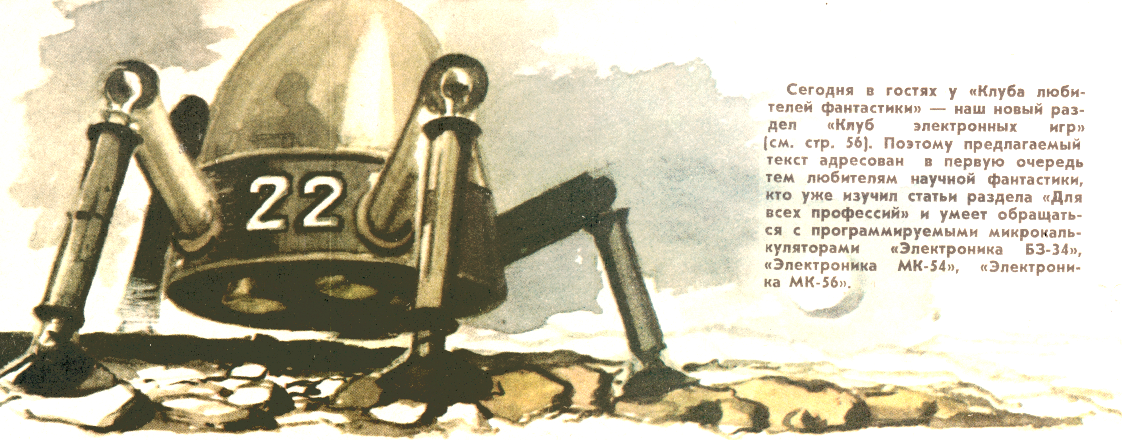
\includegraphics[width=0.5\textwidth]{real_truth}

"Громадный метеорит врезался с космической скоростью в наш звездолет и пробил его насквозь, оставив в обшивке дыру размером с человеческую голову. Воздух со свистом хлынул наружу".

«Пилот наконец решился и нажатием кнопки отправил в реактор последние остатки топлива. На космонавтов обрушилась десятикратная перегрузка. Тысячетонная громадина корабля дрогнула и медленно двинулась вверх. Люди были спасены».

Подобными эпизодами изобилуют поступающие в редакцию «ТМ» рассказы начинающих фантастов. Рецензировать такие произведения затруднительно. Интуитивно ясно, конечно, что после столкновения с «громадным метеоритом" от звездолета ничего не останется, а «последних остатков топлива» не хватит, чтобы даже при «десятикратной перегрузке» обеспечить взлет «тысячетонной громадины корабля» со сколько-нибудь приличной планеты. Но какими аргументами подкрепить интуитивные соображения? Не будешь же каждый раз проделывать громоздкие вычисления по соответствующим формулам — рассказов в отдел фантастики приходит ежедневно около десяти. Где взять время для этих проверок?

К счастью, в нынешнем году на страницах журнала открылась новая рубрика «Для всех профессий», и в редакции появился программируемый микрокалькулятор «Электроника МК-54». Поскольку ошибки наших авторов легко подразделить на несколько четко выраженных классов, я составил десяток программ для ПМК, в которые заложены наиболее типичные фантастические ситуации. Вводя в машинку различные соображения относительно размеров «громадного метеорита» и величины его «космической скорости», через минуту я получаю число, на основании которого со спокойной совестью отвечаю: «К сожалению, при самых оптимистических предположениях насчет размеров и скорости придуманного Вами метеорита диаметр проделанной им дыры в обшивке значительно превысил бы длину звездолета, то есть последний попросту превратился бы в пар, так что увлекательные приключения Ваших героев после такого столкновения никоим образом не могли иметь места. Рукопись возвращаем..."

Есть среди моих проверочных программ и такая, которая рассчитывает взлет с безатмосферных планет и посадку на их поверхность. Тот, кто внимательно изучил материалы рубрики «Для всех профессий», разберется в ней без труда. Вот эта программа:

00. ИПД 01. Fx<0 02. 09 03. ↑ 04. ИП8 05. ÷ 06. \XY 07. ПП 08. 90 09. ИПА 10. Fx≠0 11. 43 12. Fx<0 13. 33 14. 2 15. X 16. ↑ 17. ИП4 18. ИП3
19. 	— 20. X 21. ИПВ 22. $Fx^{2}$ 23. + 24. F√ 25. ИПВ 26. — 27. ÷ 28. ↑ 29. ИП8 30. X 31. БП 32. 90
33. 	ИПД 34. Fx≠0 35. 86 36. ИП3 37. $Fx^{2}$ 38. F√ 39. ИП7 40. — 41. Fx<0 42. 87 43. ИПВ 44. ИПА
45. С/П 46. П1 47. П2 48. Fx≠0 49. 43 50. ÷ 51. П8
52. 	ИП5	53.	ИПД 54. + 55. ÷ 56. ИП6 57. X 58. П3
59. ИП4	60.	— 61. ИП2 62. X 63. ИПВ	64.	+ 65. ПВ
66. FBx 67. + 68. 2 69. ÷ 70. ИП2 71. X 72. ИПА
73. 	+ 74. ПА 75. ИПС 76. ИП2 77. ИПО 78. X 79. — 80. ПС 81. ИПД 82. ИП1 83. — 84. ПД, 85. В/О
86. ИП6	87.	ИП9 88. С/П 89. Сх 90. П1 91. XY 92. П2
93. 	Fx<0 94. 50 95. ИПЗ 96. БП 97. 59

Подробная инструкция к этой программе (условно она называется «Лунолет-1») и описание увлекательной компьютерной игры, в которую можно играть с ее помощью, приведены на стр. 56. Но вернемся к проверке поступающих в редакцию материалов.

Надо сказать, что, помимо многочисленных писем, к нам довольно часто приходят посетители. Как правило, это весьма необычные люди. Один несет новый проект или действующую модель вечного двигателя либо безопорного движителя; другой рассказывает о встречах со «снежным человеком» и чудом дотянувшими до наших дней мезозойскими динозаврами. А года два назад в редакции появился человек, который категорически утверждал, что он якобы... провалился к нам из будущего, из конца XXI века!

Этот человек бывал у нас на протяжении двух недель. И каждый раз рассказывал что-нибудь о будущем. Мы внимательно все выслушивали (так полагается по долгу службы), записывали его рассказы на магнитофон. Ничего, впрочем, особенного в них не было — любой из нас при желании мог придумать и не такое. Да и как проверить? Потом он куда-то пропал, и вскоре все забыли о нем.

А недавно возникла мысль: теперь, когда у меня есть мои проверочные программы, я могу с помощью ПМК проанализировать и рассказы этого человека. Ведь все записано на пленку, а пленки хранятся в архиве!

Какое-то время ушло на розыски и подготовительную работу. И вот передо мной расшифровка старой магнитофонной записи. Рядом — готовая к вычислениям «Электроника».

Приготовьтесь и вы. Введите в свой ПМК программу «Лунолет-1» и переведите машинку в режим вычислений. Будем работать вместе.

Вот одна из его историй. (В скобках — наши краткие комментарии.)

Я управлял космическим кораблем один-единственный раз в жизни.

Конечно, в юности, как и многие мои сверстники, я мечтал стать космонавтом. Но мечты эти развеялись на первой же медкомиссии: при перегрузках больше трех «же» мне становилось плохо. А тех, кто не выдерживал пятикратной, к дальнейшим испытаниям не допускали. Волей-неволей пришлось забирать документы. Я подал на вычислительную технику, через шесть лет благополучно защитил диплом и — ирония судьбы! — был направлен по распределению на Луну, в Центр имени С. П. Королева. Там я работаю до настоящего времени.

После того как по соседству нашли неорганическую нефть, Центр сильно разросся. Теперь это настоящий город с населением порядка трех тысяч человек. Прикрывающие его купола соединены туннелями. Как в метро, только стены прозрачные. Это, грубо говоря, большие трубы, протянутые прямо по лунной поверхности. Один из туннелей ведет к астровокзалу. Космопорт Центра — обширный комплекс, он обслуживает всю Солнечную систему. По роду работы я часто бываю в порту, потому что корабли напичканы электроникой, рано или поздно что-нибудь выходит из строя, а чинить вычислительную технику — это моя специальность и прямая обязанность.

Случай, о котором я упомянул, произошел летом 2087 года. Работа у нас строится циклически: четыре месяца трудимся, два отдыхаем. Как правило, на Земле. Родные тоже прилетают иногда погостить — пассажирская линия Земля — Луна открылась давно. В то лето ко мне прилетел сын, Сергей. Я не видел его несколько месяцев, за это время он сильно подрос. Ему скоро двенадцать, и он бредит космонавтикой. Мы с женой надеялись, что самостоятельное путешествие на Луну очень его обрадует. Да и сам он, как она сообщила, в ночь накануне вылета совсем не спал.

Но когда я встретил его на астровокзале, он выглядел разочарованным.

— Ерунда! — сказал он. — Сидишь в кресле, стюардесса носит конфеты и воду в тюбиках. Как в самолете. Никаких перегрузок. Хоть и невесомость, но плавать по воздуху запрещают. Заставляют сидеть в кресле да еще и пристегиваться. Вот если бы самому в рубке сидеть за штурвалом и нажимать рычаги...

Он горько вздохнул и грустил минут пять, пока мы добирались домой. Потом отправился погулять. Вернулся через полчаса, разочарованный еще больше: на поверхность не выпускают, скафандр не дают, все кругом самое обычное, деревья и люди как на Земле. Никакой Луны нет. Разве что тяжесть поменьше, но это ему неинтересно — после двух-то суток невесомости на борту лайнера. Было уже поздно, и я уложил его спать, А потом и сам лег — завтра с утра на работу. Я пообещал взять его с собой: там интересно — вычислительные машины, манипуляторы и прочее.

Но наутро мне позвонили — появилось срочное дело. Я все записал, потом сварил кофе. Сергей был уже на ногах. Когда мы позавтракали, я сообщил, что планы изменились, так что пусть пока посидит дома. Он сначала возмутился, но потом смирился с необходимостью. Я пояснил, что буду в отсутствии каких- нибудь полтора часа.

— Папа! — сказал он. — А куда ты пойдешь?

— На космодром.

— A, — он разочарованно махнул рукой. — Я там уже был. Там скучно. Никуда не пускают.

— Мне не в порт, — объяснил я. — Мне на местные линии. Это небольшая площадка в стороне от главного поля. Лайнеров, на каком ты летал, там нет. Только лунолеты местного сообщения.

— Настоящие? — заинтересовался он.

— Разумеется, не игрушечные. Но они маленькие — всего две тонны сухого веса. Вернее, сухой массы. Здесь ведь все весит в шесть раз меньше, чем на Земле.

— Знаю, — отмахнулся Сергей. — А что ты там будешь делать?

— Работать, — пожал я плечами. — На одной из этих машин отказал киберпилот. Надо посмотреть. Если какой-нибудь пустяк, сделаю на месте. А если что-то серьезное...

— Ты пойдешь в рубку? — Глаза у него расширились.

Я невольно расхохотался.

— Какая там рубка! Кабина, два кресла. Не повернешься.

— Но приборы там? — продолжал он допрос. — Рычаги управления там?

— Конечно, — простодушно признался я. — Где же им быть еще?

— Возьми меня с собой, — потребовал он.

— Но это не игра, — попробовал я объяснить. — Это работа...

— Папа! — сказал он. — Ты мне обещал.

— Только не говори маме, — попросил я, сдаваясь.

Несколько минут спустя электрокар мчал нас по направлению к космопорту. Улицы в этот час были пустынны — все на работе. Незадолго до астровокзала мы свернули в боковой туннельчик, ведущий к служебному выходу. Сергей был в приподнятом настроении, что-то напевал.

На проходной я показал удостоверение вахтенному.

— А это что за гражданин?

— Он со мной, — сказал я. — Это мой сын.

— А где его документ? — спросил вахтенный.

— Ему не положено. Он еще маленький.

Минуту вахтенный размышлял. Ситуация, очевидно, была для него новой.

— Ладно, пускай идет. Под личную ответственность.

Скафандры нам выдали без проблем. Сережке, конечно, он был великоват, но только чуть-чуть —не такой уж он у меня маленький.

— Баллоны стандартные, — предупредил выпускающий. — На два часа. Справитесь?

— Конечно. Мне и часа хватит с гарантией. Двадцать минут туда, двадцать обратно, десять на месте. Ну и десять на всякие осложнения.

— Ясно, — добродушно сказал выпускающий. — Только пусть лучше осложнений не будет. Хорошо?

Я опустил забрало, и мы прошли в воздушный шлюз. А спустя короткое время уже шагали под голубым светом Земли. Была середина лунной ночи — на Земле в эти дни новолуние.

Сказать, что Сергей был восхищен, — значит, ничего не сказать. Он был ошеломлен. Похоже, он никак не ожидал, что ему выдадут скафандр. Настоящий, с индивидуальной системой жизнеобеспечения. На Земле я бы в таком весил килограммов сто пятьдесят, да и Сергей потянул бы на добрую сотню. Мы осторожно шагали по ровному реголиту — искусственного покрытия здесь никто не прокладывал, убрали крупные камни, и все. Не для важных персон. Но дорожка была ухоженной. До нас здесь ходили многие — все, кто работал на дальних лунных базах и опорных пунктах. Строители, ученые, инженеры...

— А там что такое? — Сергей вновь обрел способность задавать вопросы. Его голос в моем шлемофоне звучал непривычно.

Он показывал направо. Там выступали из-за горизонта массивные строения промышленного блока.

— Это тебе неинтересно, Сережа, — сказал я. — Там качают нефть и гонят из нее керосин. Для двигателей. — Я махнул в сторону космопорта. — И еще вырабатывают жидкий кислород.

— Для скафандров? — Он произнес слово «скафандр» с особенным выражением. Я усмехнулся:

— И для скафандров, конечно. Но в основном его везут на те же заправочные станции. Горючее ведь не будет гореть без окислителя.

Некоторое время мы шагали в молчании. Идти стало чуть труднее — дорожка поднималась к вершине обычного для Луны плоского холма. Еще сотня шагов — и мы достигли места своего назначения. Нашим глазам открылась стоянка лунолетов.

Их было десятка два — старые, но надежные машины. В первом приближении это скругленный конус высотой метра три с половиной, опирающийся на четыре амортизатора типа «паучья нога». Вся верхняя часть прозрачна, для облегчения обзора. Это и есть та самая «рубка», в которую так рвался мой сын.

На боку каждого лунолета стоял опознавательный номер — две цифры, начертанные светящейся краской и обведенные черной каймой. Наш был с краю. Без дополнительных приключений мы забрались внутрь. При виде многочисленных циферблатов у Сергея разгорелись глаза.

— Это настоящий корабль? — спросил он.

Я понял. На Земле похожие машины стоят в каждом парке отдыха. Аттракционы. Влезай в люк и испытывай всякие ощущения.

— Самый что ни на есть, — сказал я.

— А как им управлять?

Я усмехнулся.

— Проще простого. Вот этот ящик, — я указал пальцем, — называется киберпилот. Если тебе нужно попасть, допустим, на базу «Циолковский», ты набираешь на пульте задание, потом нажимаешь вот эту кнопку, и киберпилот благополучно доставляет тебя куда надо. Но сейчас именно он-то и неисправен.

Это Сергея на время утихомирило. Он, видимо, ожидал чего-нибудь в духе земных аттракционов, когда сам даешь вводные и тебя швыряет в разные стороны. Я аккуратно снял с киберпилота пломбу и сдвинул лицевую панель. На вид все в порядке. Дал на схему напряжение. Циферблаты на пульте ожили.

Где же искать повреждение?..

— А это что за рычаги? — услышал я голос Сергея.

Я обернулся. Оказывается, он устроился во втором кресле. Играл в космонавта. Указывал он на рычаги ручного управления двигателем.

— Это для посадки, — объяснил я. — Киберпилот всегда доставит тебя куда надо, но он не знает местность. Вдруг там трещина, скажем, или какой-нибудь камень. Тогда нужно дать небольшой импульс, чуть притормозить спуск, чтобы машина проскочила опасное место.

Я опять повернулся к киберпилоту. Однако не тут-то было.

— А как дать импульс? — спросил Сергей.

— Ты мне мешаешь, — сказал я. — Откуда мне знать? Впрочем, гляди: написано «Расход топлива» и цифры, ага, в килограммах. Рычаг стоит здесь, значит, ты собираешься истратить 65 килограммов топлива. А возле правого рычага — «Время» и тоже цифры. Это, видимо, время, за которое ты собираешься свое топливо израсходовать. Меньше время — больше тяга, а если время больше — тяга соответственно меньше. Сейчас рычаг стоит на цифре три. Значит, если ты подашь эту команду на двигатель, он израсходует 65 килограммов за три секунды.

— А это много?

— Не знаю, — сказал я. — По-моему, все равно что ничего.

— А как подать команду на двигатель?

— Откуда я знаю? — огрызнулся я. — Ты мне мешаешь. Пульт наверняка заблокирован, а баки пусты. Полюбуйся, — я ткнул пальцем в индикатор, — Видишь? «Топливо», четыреста. Всего-навсего! А шкала на две с половиной тонны.

— А как... — продолжал он допрос.

— Отстань от меня! — скомандовал я. — Ты мне мешаешь. Скажешь еще хоть слово, тут же идем домой. И вообще, отошлю тебя к маме.

Он обиженно умолк, а я занялся киберпилотом. Набрал контрольный тест — он прошел нормально. Набрал второй — тоже полный порядок. Что они там, спятили? Совершенно исправная машина. Я набрал третий тест. И тут началось...

\textbf{
(Пока рассказчик работает с вычислительной техникой, поработаем немного и мы. Не будем забывать о своей главной задаче — вывести его на чистую воду. Кульминационный момент, судя по всему, приближается, самое время нажимать клавиши ПМК. Программа введена, формируем и отправляем в регистр 9 аварийный сигнал Г: Сх ÷ ВП ВП ↑ П9. Теперь исходные данные. Дело происходит на Луне, ускорение свободного падения 1,62 м/c$^{2}$. Набираем на клавиатуре 1,62 П4. Масса корабля без горючего две тонны, сюда нужно добавить массу рассказчика вместе со скафандром (150 кг) и его сына (100 кг). Набираем 2250 П5. Двигатель, очевидно, работает на керосине и жидком кислороде, скорость истечения 3660 м/с. Набираем это число на клавиатуре и нажимаем П6. Очередь за предельным ускорением. По словам рассказчика, ему становится плохо уже при трех «же». Набираем на клавиатуре 9,81 ↑ 3 X П7. Скорость и высота равны нулю — нажимаем 0 ПА ПВ. Запас топлива 400 кг. 400 ПД. Вводим в регистр С ресурс жизнеобеспечения в секундах. Воздуха в баллонах было на два часа, двадцать минут герои повествования шли до стоянки, возятся минут двадцать, да надо еще накинуть двадцать на обратный путь. «На всякие осложнения» им остается ровно час. Набираем 3600 ПС и соответственно I ПО. Исходные данные введены. Нажимаем В/О и С/П. Через секунду на экране загорается высота — ноль. Нажимаем XY. На экране скорость — тоже ноль. Все правильно. Можно во всеоружии ждать грядущих событий. А они, несомненно, вот-вот последуют.)
}

...Ни один контрольный тест не проходил. Я бросил взгляд на часы: с момента, когда мы покинули воздушный шлюз, прошло уже сорок минут. Пора возвращаться. Я потянулся к рубильнику — снять с оборудования напряжение — и посмотрел на сына. Он продолжал играть в космонавта: нажимал какие-то кнопки,. созерцал пляшущие на экранах кривые. Рычаги управления тягой стояли в прежнем положении. Он положил указательный палец на большую красную клавишу. Неясное предчувствие шевельнулось у меня в голове.

— Не смей! — крикнул я.

Но было поздно. Под нами загрохотало, за прозрачным колпаком взметнулось пламя, чудовищной силы удар швырнул меня в кресло, и у меня потемнело в глазах...

\textbf{
(Значит, пульт все-таки заблокирован не был и команда прошла на двигатель. Не особенно, конечно, убедительно, но нас интересует фактическая сторона дела. Двухтонная машина, жалкие 60 кг топлива, и вдруг — «чудовищной силы удар»! К счастью, проверить данный эпизод нетрудно. Подадим ту же команду и на свой пульт: 65 ПП 3 С/П. На экране мелькают цифры, потом... загорается аварийный сигнал Г! Как это ни удивительно, перегрузка действительно превысила допустимую, рассказчик потерял сознание и какое-то время после отсечки двигателя не сможет управлять лунолетом. Снова нажимаем С/П.)
}

...Когда я очнулся, кругом было только небо. Сколько я был без сознания? Не знаю. Но мы падали, падали со страшной скоростью! Очевидно, за время моего беспамятства ракета прошла вершину траектории и теперь стремительно неслась вниз. Сергей тянулся к рычагам управления. Но игры кончились. Какую-то секунду я не мог опомниться, но еще через секунду был у пульта. Что я мог успеть в такой ситуации? Заметил лишь показания индикаторов — скорость восемьдесят, высота триста с чем-то.

— Папа! - крикнул Сергей.

Что я мог успеть? Не меняя режима двигателя, я ударил по красной клавише. На нас снова обрушилась перегрузка...

\textbf{
(На нашем же индикаторе высота полета 169 м — везде округляем до целых. Нажимаем XY. Скорость 84 м/с. Ну что ж, будем считать, проверка закончена. Скорость еще более-менее, но высота в рассказе завышена вдвое. Можно откладывать ПМК в сторону... Впрочем, пока он добирался до пульта, прошло еще две секунды. Две секунды свободного падения с выключенным двигателем. Но куда можно упасть за две секунды? Разве что на Луну — не в небо же! Ладно, для очистки совести засылаем соответствующую команду: 0 ПП 2 С/П. На экране зажигаются высота 334, скорость 81. Невероятно, но цифры совпали! Почему же он утверждает, что лунолет падал? Непонятно. Но набираем новую команду: 65 ПП 3 С/П. Опять сигнал Г — запредельные перегрузки! — вновь нажимаем С/П и ждем результата.)}

...Когда я очнулся снова, мы опять падали. Я рванулся к красной клавише, но взгляд мой упал на индикатор высоты. Почти километр! И цифры росли! Значит, мы вовсе не падали — мы неслись вверх со скоростью реактивного истребителя! И в прошлый раз мы, конечно же, тоже поднимались! Меня ввела в заблуждение невесомость. Мы действительно падали, но падали вверх! И я, болван, включив двигатель, только усугубил наше и без того тяжелое положение. Зато теперь появилось время, чтобы собраться с мыслями...

\textbf{
(Не так-то просто, оказывается, поймать его на слове! У нас очередной останов. Высота 916 м — действительно, почти километр, —- скорость 166 м/с. Примерно 600 км/ч. Маловато, конечно, для истребителя, но... Можно ли считать это серьезной ошибкой? Будем объективны, оставим рассказчику право на художественное преувеличение. Как бы то ни было, включать двигатель он вроде цока не собирается, так что нашему ПМК можно тоже дать передышку.)}

...— Папа! — сказал Сергей, выбираясь из-под меня. — А почему ты говорил, что 65 килограммов — это все равно что ничего?

— Отстань от меня! — приказал я, — Марш во второе кресло и пристегнись!

Я проследил, как он это выполнил, и пристегнулся сам. Цифры на индикаторе высоты увеличивались, но все медленнее и медленнее. На киберпилот надежды нет, придется выкручиваться самому. Но пока, пожалуй, лучше не делать ничего. Гнать вверх бессмысленно. Вниз (а рядом с красной клавишей я углядел другую, «Реверс тяги») — еще хуже. Вот начнем падать, тогда... Я заранее установил рычаги в положение 25 кг и 2 с и ждал. Да, я сильно ошибся насчет этих килограммов. Похоже, в них большая сила...

— Папа! — подал голос Сергей. — А мы сможем улететь в космос?

— Отстань! — рявкнул было я, но вдруг у меня защемило сердце. Ребенок не понимал, что мы на волосок от гибели, для него это было игрой! — Сереженька, — сказал я как можно ласковее, — в космос мы с тобой еще слетаем. Но сейчас, пожалуйста, помолчи...

Мы взлетели уже почти на десять километров. Цифры на указателе скорости дошли до нуля и начали медленно расти, теперь уже с отрицательным знаком. Когда скорость достигла примерно тридцати метров в секунду, я нажал красную клавишу. Высота к этому времени уменьшилась почти до девяти километров. Свободный полет продолжался ровно две минуты...

\textbf{
(Наконец-то появилась новая цифра, которую можно проверить. Две минуты с нулевой тягой. Команда: 0 ПП 120 С/П. После останова высота 9175, скорость — минус 28. Опять все сходится! Новая команда: 25 ПП 2 С/П. Машинка рассчитывает маневр.)}

...На сей раз перегрузка была терпимой. На индикаторах мелькали цифры. Высота почти не изменилась, но мы опять поднимались! Что ж, мы так и будем болтаться на этой высоте, пока не кончится все топливо? И весь кислород?! В отчаянии я установил рычаги в положение 10 и 10 и дал реверс тяги. Лунолет кувыркнулся двигателем вверх. Далеко внизу я увидел постройки Центра, обширные поля космодрома и крошечное пятнышко площадки, с которой мы так неосмотрительно стартовали...

\textbf{
(У нас после останова высота 9151, скорость — чуть меньше пяти метров в секунду и, действительно, снова направлена вверх. Вводим команду 10 ПП 10 ПП /—/ С/П. После останова высота равна 9044 м, скорость — 26 м/с со знаком минус. Снова падаем, и довольно быстро.)}

...Скорость падения увеличивалась быстрее, чем я рассчитывал. Я решил притормозить: убрал реверс, установил 25 кг и 5 с и надавил на красную клавишу. Но она не поддалась. Видимо, эти пульты устроены так, что новая команда блокируется, пока не исполнена прежняя. И лишь когда десять секунд истекли, корабль вновь крутанулся двигателем вниз. Но когда тот выключился, мы оставались все на тех же девяти километрах и опять, хоть и очень медленно, поднимались!..

\textbf{
(Команда: 25 ПП 5 С/П. Результат: высота 8984, скорость два с половиной метра в секунду, снова со знаком плюс. Он что, действительно собирается провести здесь всю оставшуюся жизнь?)}

...Нет, решил я, так дело не пойдет. Если мне даже удастся установить приемлемую скорость спуска — допустим, пять метров в секунду, — и поддерживать ее до самого прилунения, то сколько времени на это уйдет? Полчаса? Час? Топлива не хватит наверняка. Да и кислород...

— Папа! — вновь подал голос сын. — Топлива всего двести...

— Двести десять! — рявкнул я. — Но помолчи же!

Мы уже снова падали — все быстрее и быстрее. Топлива осталось чуть больше половины. Но если, черт побери, на половине топлива мы ухитрились забраться сюда, то оставшейся половины должно хватить для возвращения! Если, конечно, его разумно тратить... Только как это — разумно?

Я решил выждать сколько возможно, а потом дать резкий тормозной импульс. Заранее установил рычаги в положение 100 и 3. На этот раз свободный полет продолжался полторы минуты. Мы уже опять неслись со скоростью истребителя, но только вниз. До поверхности оставалось чуть больше двух с половиной километров, когда я надавил красную клавишу. На нас вновь обрушились перегрузки...

\textbf{
(Полторы минуты свободного падения. 0 ПП 90 С/П. - Высота 2652, скорость падения 143. Около 500 км/ч. Но сравнение с истребителем, как мы договорились, не ошибка, а всего лишь гипербола. Вводим 100 ПП 3 С/П. На экране, естественно, буква Г. Перегрузки снова превысили допустимую величину. Не слишком ли часто? Но нажимаем С/П. Высота 2123, скорость минус 32.)}

...Когда вернулось сознание, высота упала на полкилометра, но скорость снизилась до тридцати метров в секунду. Маневр удался! Можно попробовать идти дальше с этой же скоростью, а где-нибудь ближе к поверхности повторить маневр. Только как удержать скорость? Я решил экспериментально подобрать нужную тягу. Для начала дал 10 кг за 20 с. К нам снова вернулся вес — правда, поменьше, чем на Луне, — но скорость все-таки росла. К окончанию маневра она достигла 50 метров в секунду. Я увеличил тягу: те же десять килограммов, но теперь за 15 с...

\textbf{
(Повторяем оба маневра. 10 ПП 20 С/П. Высота 1314, скорость спуска 49. 10 ПП 15 С/П. Высота 515, скорость 58. Многовато!)}

...Скорость все равно увеличивалась, а до лунной поверхности оставалось каких-нибудь полкилометра. Запас топлива — 80 килограммов. Делать было нечего. Я дал 35 кг за полторы секунды — и, конечно же, вновь отключился...

\textbf{
(Команда: 35 ПП 1,5 С/П. На экране Г — перегрузки. С/П. Результат: высота 390, скорость спуска 17. Примерно 60 км/ч. Это уже полегче.)}

...Когда я пришел в себя, то понял, что маневр удался. До поверхности было еще почти 400 метров, а скорость упала больше чем втрое! Семнадцать метров в секунду — скорость электрокара! Я знал уже, как ее сохранить. Я заслал 22 кг за 22 с. Сам я родился 22 марта. Сергей родился, когда мне было 22 года. И вообще, 22 — число для меня счастливое...

\textbf{
(Команда: 22 ПП 22 С/П. На экране мелькают цифры.)}

...Я действительно угадал! Скорость почти не менялась, только в десятых долях. Высота равномерно уменьшалась: 250... 200... 150... 100... 50... И вдруг до меня дошло, что мы вот-вот врежемся в поверхность Луны, амортизаторы не удержат! Топлива оставалось 33 кг. Оставив рычаг расхода на прежней отметке, я рванул второй вниз до упора — 0,7 с — и давил, давил, давил на красную клавишу. Но она поддалась, лишь когда до гибельного удара осталось меньше секунды. Опять перегрузки...

\textbf{
(На экране: высота 13,5, скорость 17,5. Команда: 22 ПП 0,7 С/П. Г — перегрузки! Снова С/П.)}

...Как ни удивительно, но я, видимо, отключился лишь на ничтожную долю секунды. Когда сознание вернулось ко мне, скорость была прежней, а от поверхности нас отделяли всего 7 метров. Двигатель молчал. Впоследствии я не раз задумывался, как такое могло случиться. Неужели сбой двигателя? Не знаю. Но в тот момент мне было не до размышлений. Палец лежал на клавише. Я повторил команду, послав в двигатель последние капли топлива. Я сделал это в тот же миг, как открыл глаза. Новый удар ускорений...

\textbf{
(Высота 7, скорость 17. Все сходится! Но не могли же одновременно подкачать и двигатель лунолета, и наша «Электроника»! Попробуем разобраться в ситуации — у нас-то время есть. Проверяем запас топлива. ИПД. На индикаторе 11 кг. Значит, двигатель свои 22 кг отработал. Почему же тогда прежняя скорость? Смотрим время, на которое выключался двигатель. ИП2. На экране 21 с. Ничего себе, «ничтожная доля секунды»! Впрочем, и это нельзя считать неточностью рассказчика: выглядело-то все именно так, а откуда ему знать, сколько он был без сознания? У него ведь нет такой аппаратуры, как наша! А произошло следующее: расход был задан слишком большой, двигатель не только полностью погасил скорость, но и вновь разогнал лунолет вверх. И только после этого выключился на 21 секунду, за это время Луна вновь подтянула корабль к себе. А он думает, «сбой двигателя»! Но ладно, вводим последнюю команду: 22 ПП 0,7 С/П. Да, но ведь топлива осталось всего 11 кг, а задано 22! На индикаторе загорается буква Г. Перегрузки? На этот раз машина сигнализирует о более важном происшествии: команда на двигатель подана с превышением наличного запаса топлива. Когда оно иссякнет — а это случится «ровно через 0,35 с, — он выключится окончательно. Нажимаем С/П. На экране мелькают цифры, и вдруг загорается ноль. Поверхность! Смотрим скорость: 3,7 м/с. Отличная посадка!)}

...Двигатель молчал. Я лежал в кресле в ласковых объятиях привычного лунного тяготения. Лунолет, покачиваясь на амортизаторах, стоял невдалеке от того места, откуда мы стартовали. На индикаторах застыли скорость — меньше четырех метров в секунду — и время — 350. Значит, мы летали неполные шесть минут...

Я повернул голову — как там мой Сергей? Он лежал неподвижно, глаза его были закрыты.

— Сережа, — позвал я.

Он не шелохнулся.

— Сережа! — заорал я. Он оставался недвижен.

Я рванулся из кресла — меня не пустили ремни. Не помню, как я расстегнул пряжки, как очутился с ним рядом. Я тряс его, дергал — безрезультатно. Не знаю, сколько это продолжалось. И вдруг...

В моем шлемофоне раздался его громкий счастливый смех!

Он продолжал играть! Он играл в космонавта, убитого перегрузками!..

Потом, конечно, я многим рассказывал об этом приключении. Все, само собой, изумлялись, как это мне, впервые оказавшемуся за пультом, удалось выполнить столь успешную посадку. Только один приятель, по профессии селенолог, выслушал все внимательно и произнес: «Неплохо! Но мне, я думаю, в такой ситуации хватило бы и шестидесяти!» Он имел в виду, что затратил бы на посадку не триста с чем-то килограммов топлива, как я, а всего шестьдесят. Я не понимаю, как это можно сделать — ведь на старте было сожжено шестьдесят пять, значит, и на финиш должно уйти минимум столько же! Однако в подробности он вдаваться не стал. Хватило бы, и точка! Эти селенологи лихие ребята — гоняют на своих лунолетах по всей Луне. Им виднее.
Сережка, разумеется, тоже хвастался всем подряд. Его версия происшедшего звучала примерно так: «Папа посадил корабль на Луну, зато в космос поднял его я!» Друзья, конечно, сильно ему завидовали.

И только маме он ничего не сказал. Потому что пообещал.

\textbf{
(Рассказ подошел к концу. Но, собственно, и наша работа закончена. Отодвигаем ПМК в сторону. Какие неточности удалось обнаружить? Никаких. Так, парочку преувеличений. А проверить такие факты, как последний, наша программа не в состоянии...
Если же кому-нибудь захочется выяснить, прав ли был тот лихой селенолог, сделайте это сами. Закачивайте топливо в баки и дерзайте. Но только, пожалуйста, не забудьте перед стартом уменьшить массу лунолета на 100 кг. Вот так: ИП5 100 — П5. Пока не приобретете опыта, не берите с собой ребенка!)}

\section{мягкой посадки!}
Консультант раздела — Герой Советского Союза, летчик-космонавт СССР Ю. Н. Глазков

Электронно-фантастическая игра для ПМК класса «Электроника БЗ-34»

\begin{figure}[H]
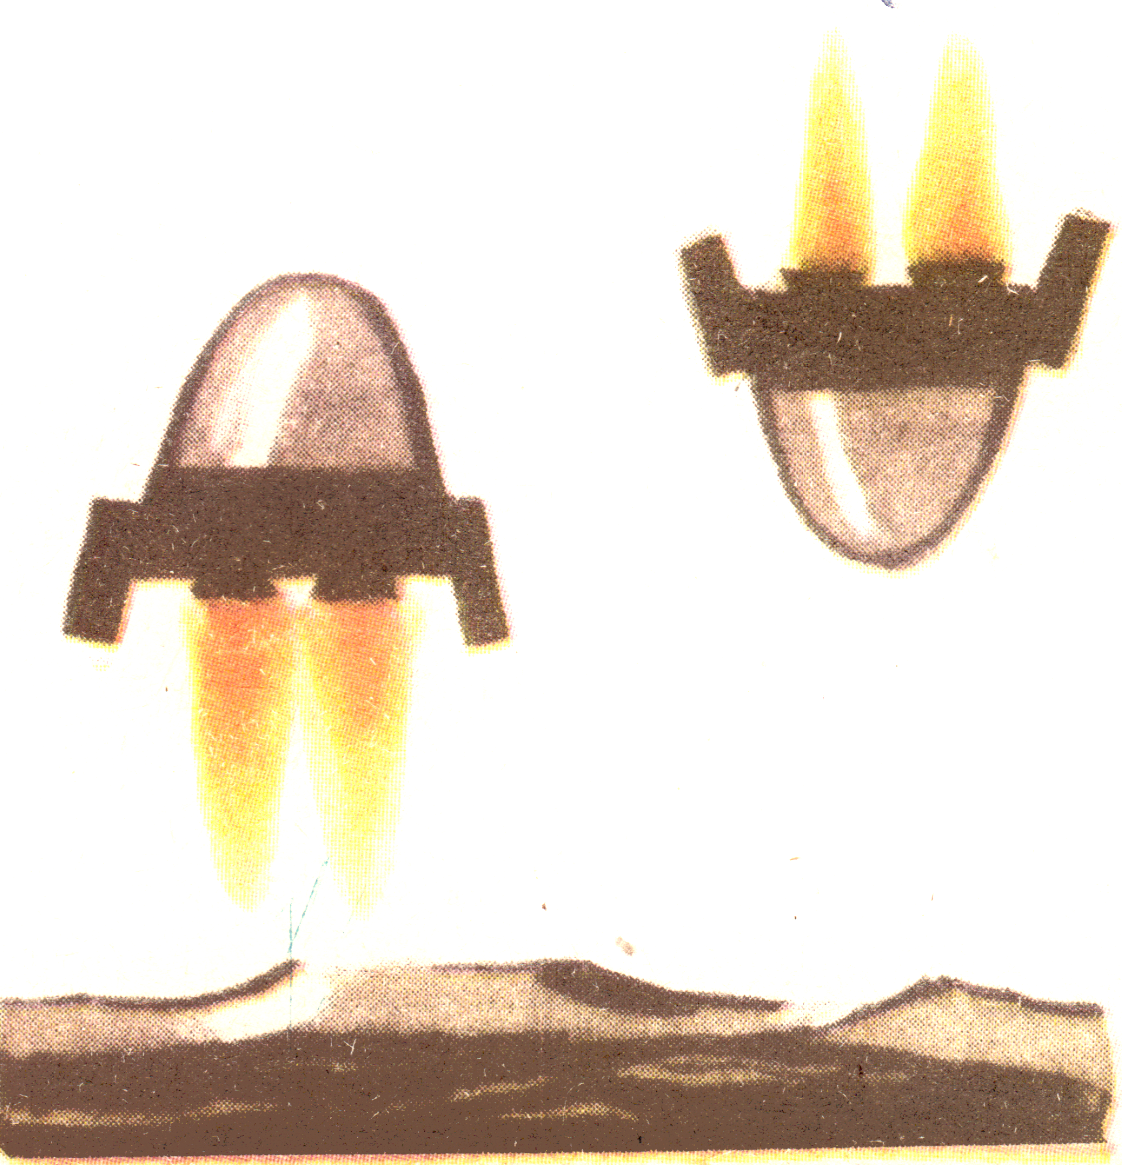
\includegraphics[width=0.5\textwidth]{lunolet1_orientation}
\caption{Нормальное торможение. Для передачи на двигатель заданного с пульта режима нужно нажать С/П (слева). Реверс тяги. Для передачи на двигатель заданного режима нажать ПП /—/ С/П (справа).}
\end{figure}

Программа «Лунолет-1» (см. стр. 52/*FIXME*/) может использоваться не только для численного моделирования маневров космических аппаратов в непосредственной близости безатмосферных небесных тел или в качестве учебного пособия, но и как основа ряда электронных игр для программируемых микрокалькуляторов. Сегодня мы знакомим читателей с одной из них. Играющий должен, регулируя тягу двигателя, посадить корабль на планету, причем скорость в момент контакта с поверхностью не должна превышать выбранного значения, например 5 м/с (мягкая посадка). Чтобы играть в эту игру, нужно после ввода программы в ПМК выполнить следующие подготовительные операции:
\begin{enumerate}
\item Сформировать и заслать в регистр 9 аварийный сигнал. Например, букву Г: Сх ÷ ВП ВП ↑ П9.
\item Ввести в память машины константы и начальные значения переменных: (ускорение свободного падения на поверхности планеты, м/с$^{2}$) П4; (масса корабля без топлива, кг) П5; (скорость истечения продуктов сгорания, м/с) П6; (предельное ускорение, которое могут выдержать космонавты, не теряя сознания, м/с$^{2}$) П7; (начальная высота, м) ПА; (начальная скорость, м/с, причем положительным считается направление вверх) ПВ; (запас топлива, кг) ПД.
\end{enumerate}

В регистре С может откладываться либо текущее время, либо время, оставшееся до установленного срока (например, если ресурс жизнеобеспечения ограничен). Для реализации первого варианта нужно набрать команду: 0 ПС 1 /—/ П0; для реализации второго: (ресурс, с) ПС 1 П0. Если же играющего время не интересует, регистры С и 0 можно не задействовать.

Все исходные данные вводятся в произвольном порядке.

Теперь нужно нажать В/О и затем С/П. Игра началась. Каждый ход можно подразделить на два этапа: анализ ситуации и ввод исходных данных для очередного маневра.

\paragraph{АНАЛИЗ СИТУАЦИИ}
При останове на экране горит значение текущей высоты полета. Командой XY на индикатор вызывается текущая скорость. После этого можно при желании вызывать из памяти любые постоянные и переменные величины (они хранятся в тех же регистрах, куда были введены соответствующие исходные данные), производить на ПМК любые расчеты. После этого можно переходить к следующему этапу.

\paragraph{ВВОД ИСХОДНЫХ ДАННЫХ ДЛЯ МАНЕВРА}

Режим двигателя при маневре определяется расходом топлива и временем, за которое этот расход произведен, и задается командой: (расход, кг) ПП (время, с). Если надо ускорить спуск, после этого отдается команда ПП /—/ (реверс тяги, см. рисунок). Реверс весьма полезен при посадках на планеты со слабой и особенно отрицательной гравитацией. Для передачи набранной команды на двигатель нужно нажать С/П и ждать появления на индикаторе очередной высоты.

Задавать время маневра равным нулю нельзя. В этом случае ускорение получилось бы бесконечно большим. Если вы ошибетесь, на экране тут же загорится прежняя высота: ПМК ждет ввода правильных данных.

\paragraph{АВАРИЙНЫЕ СИТУАЦИИ}

Если после передачи команды на двигатель на экране загорается аварийный сигнал, это означает одно из двух: либо кончилось топливо, либо ускорения превысили допустимое значение. В первом случае по завершении маневра двигатели выключатся и корабль упадет на поверхность планеты, во втором — отключатся на некоторое время (пропорциональное перегрузкам), и корабль на протяжении этого времени тоже будет свободно падать: считается, что экипаж еще не обрел способности управлять кораблем. Если был задан расход, превышающий наличный запас топлива, двигатель выключится до завершения намеченного маневра, в момент полного исчерпания топлива, причем тяга (она пропорциональна отношению расход/время) будет равна заданной.

При аварийном сигнале нужно нажать С/П. Обращаться к памяти или производить на ПМК какие-то вычисления в аварийной ситуации нельзя. Если она была связана с перегрузками, то при останове на очередной высоте в регистре 2 находится время свободного падения. Оно вызывается на индикатор командой ИП2.

Игра заканчивается, когда при очередном останове на индикаторе загорается 0 (в некоторых случаях вместо ноля может появиться небольшое положительное число, например, $1 * 10^{-5}$). Значения скорости и остальных переменных в момент посадки вызываются на индикатор теми же командами, что и в обычной ситуации. При переходе к новому варианту нужно ввести новый комплект исходных данных, причем константы, если они остались неизменными, можно не вводить. Затем нажать В/О и С/П/

Когда вы наберетесь опыта и научитесь уверенно садиться на любую планету, попытайтесь ответить на два вопроса по рассказу «Истинная правда»:
\begin{enumerate}
\item Чем можно объяснить хвастливое заявление лихого селенолога, что на посадку ему бы потребовалось меньше топлива, чем было затрачено на взлет? Какие физические явления стоят за его словами?
\item Чем принципиально отличаются ситуации, описанные на стр. 52 («Пилот, наконец, решился и нажатием кнопки отправил в реактор последние остатки топлива...») и на стр. 56 («Я повторил команду, послав в двигатель последние капли топлива...»)? Почему в первом случае у решительного пилота ничего не получится, а во втором, как мы знаем, все завершилось вполне благополучно?
\end{enumerate}

В следующем выпуске мы познакомим вас еще с несколькими электронными играми, базирующимися на программе «Лунолет-1».

\section{МЯГКОЙ ПОСАДКИ!}

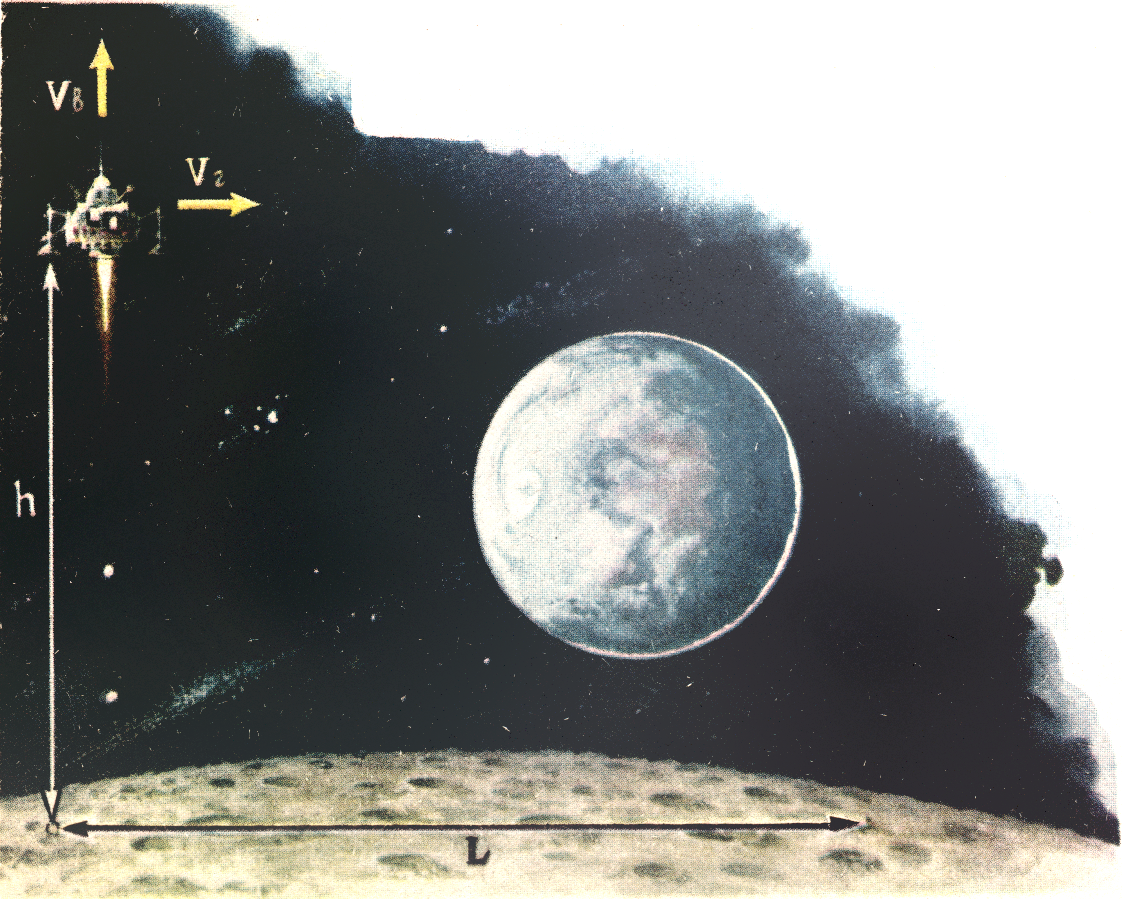
\includegraphics[width=0.5\textwidth]{soft_land1}

МИХАИЛ ПУХОВ

Новые электронно-фантастические игры для ПМК класса «Электроника БЗ-34.»

Консультант раздела — Герой Советского Союза, летчик-космонавт СССР Ю. Н. ГЛАЗКОВ

Предлагаем вашему вниманию модификацию игры, описанной в июньском номере «ТМ». Играющий должен, управляя вертикальной тягой, посадить космический корабль, движущийся с небольшой постоянной горизонтальной скоростью, в выбранную точку на поверхности планеты (см. рисунок).

Для игры используется программа «Лунолет-1», опубликованная в предыдущем выпуске. Подготовительные операции и ввод исходных данных остаются прежними. Единственное отличие — в регистр С нужно ввести начальное расстояние (по горизонтали) до точки посадки в метрах, а в регистр 0 — горизонтальную скорость в метрах в секунду. Реализуются эти операции командами: (расстояние, м) ПС (скорость, м/с) ПО.

Игра протекает точно так же, как и в уже опубликованном варианте, только при анализе ситуации полезно с помощью команды ИПС проверять текущее расстояние до точки посадки. Навыки, приобретенные при отработке посадки с постоянной горизонтальной скоростью, очень пригодятся в дальнейшем, когда нам с вами придется решать гораздо более сложные навигационные задачи. Мягкой посадки!

СДЕЛАЙ САМ СЕБЕ ПЛАНЕТУ

Одна из важных констант, используемых в наших играх, — это ускорение силы тяжести на поверхности планеты. Еще два параметра, без которых в скором будущем не обойтись, — радиус планеты и первая космическая скорость. Приводим сводную таблицу этих величин для тех небесных тел (за исключением планет-гигантов), для которых они известны более или менее точно.

Сколько-нибудь надежных данных по другим небесным телам нет. Зато планетологи установили довольно простую зависимость ускорения свободного падения от радиуса планеты, если та сложена из материалов, подобных земных. Приведем ее в виде программы для ПМК «Электроника БЗ-34»:

00.П0 01.ИПВ 02.÷ 03.ПД 04.1 05.— 06.ИПС 07.Х 08. $Fe^{x}$. 09.ИПД 10.Х
11.ИПА 12.Х 13.↑ 14.ИП0 15.Х 16.1 17.ВП 18.3 19.Х 20.F√ 21.\XY 22.С/П 23.БП 24.00

Называется эта программа «Планетный конструктор» (сокращенно «ПК-1»). Чтобы ею пользоваться, нужно после ее ввода в ПМК занести в регистр А ускорение силы тяжести на земной поверхности (в м/с$^{2}$), в регистр В средний земной радиус (в км) и в регистр С — эмпирическую безразмерную константу, равную 0,6904. Реализуются эти операции	последовательностью команд: 9,81 ПА 6371 ПВ 0.6904 ПС В/О. После этого можно приступать к конструированию миров. Задайтесь радиусом планеты, которую вы намереваетесь создать наберите на клавиатуре его величину в километрах и нажмите С/П. После останова на индикаторе светится ускорение силы тяжести на поверхности «изготовленной» вами планеты, а первая космическая скорость находится в регистре Y — она вызывается на индикатор командой \XY. Теперь можно набирать радиус очередной планеты и вновь нажимать С/П. Практика показывает, что изготовлять планеты по этой методике даже легче, чем печь, блины.

Если вы захотите испытать программу «ПК-1» на нашей таблице, выявится одна интересная деталь. Для Земли, Венеры, Марса, Луны, Ио и Европы вычисленные значения почти не отличаются от экспериментальных. А вот расчетные величины ускорения силы тяжести на Ганимеде или Каллисто почти вдвое превышают реальные. Это значит, что данные небесные тела в строгом смысле не принадлежат к земной группе — они сложены из материалов, в среднем вдвое менее плотных, чем земные горные породы. Именно на основании такого сравнения ученые пришли к выводу, что эти два спутника Юпитера примерно наполовину состоят из льда. То же самое можно сказать и о большинстве спутников Сатурна. А вот Меркурий, как нетрудно убедиться, наоборот, построен из более плотных пород — вычисленное значение силы тяжести на его поверхности в полтора раза меньше полученного экспериментально. Считается, что аномально высокая плотность Меркурия связана с его близостью к Солнцу: под действием излучения более легкие элементы покинули планету, скорее всего еще в процессе ее образования.

\begin{table}[H]
\begin{tabular}{|l|l|l|l|}
\hline
\rotatebox{90}{\thead{Название\\небесного\\тела}} & \rotatebox{90}{Радиус, км} & \rotatebox{90}{\thead{Ускорение\\силы\\тяжести,\\м/с$^{2}$}} & \rotatebox{90}{\thead{Первая\\космическая\\скорость, м/с}} \\\hline
\multicolumn{4}{l}{Планеты}\\\hline
Земля       & 6371  & 9,81 & 7905     \\
Венера      & 6056  & 8,85 & 7321     \\
Марс        & 3394  & 3,72 & 3553     \\
Меркурий    & 2440  & 3,70 & 3005     \\
Плутон      & 1500  & 0,4  & 780      \\\hline
\multicolumn{4}{l}{Спутники Юпитера}  \\\hline
Ио          & 1815  & 1,80 & 1807     \\
Европа      & 1569  & 1,32 & 1437     \\
Ганимед     & 2631  & 1,43 & 1943     \\
Каллисто    & 2400  & 1,23 & 1715     \\\hline
\multicolumn{4}{l}{Спутники Сатурна}  \\\hline
Мимас       & 196   & 0,06 & 102      \\
Энцелад     & 250   & 0,08 & 143      \\
Тефия       & 530   & 0,15 & 283      \\
Диона       & 560   & 0,22 & 351      \\
Рея         & 765   & 0,26 & 447      \\
Титан       & 2575  & 1,37 & 1881     \\
Япет        & 730   & 0,14 & 317      \\\hline
\multicolumn{4}{l}{\makecell{Луна, Тритон (спутник Нептуна),\\ Харон (спутник Плутона) и \\Фобос (спутник Марса)}} \\\hline
Луна        & 1738  & 1,62 & 1678     \\
Тритон      & 2100  & 2,0  & 2049     \\
Харон       & 650   & 0,2  & 350      \\
Фобос       & 11    & 0,007& 9       \\\hline
\end{tabular}
\end{table}

УГАДАЙ ТЯГОТЕНИЕ!

Теперь, когда у вас появилась возможность конструировать по своему желанию планеты с любой гравитацией, вы можете сыграть в еще одну игру, базирующуюся на программе «Лунолет-1». Играют в нее двое. После введения в ПМК программы и комплекта исходных данных один из играющих (естественно, втайне от другого) вводит в регистр 4 ускорение силы тяжести на поверхности планеты, которую он загадал (планета может быть реально существующей или изготовленной на «Планетном конструкторе»). Начальные скорость и высота полета задаются равными нулю, а запас топлива — достаточным для взлета, непродолжительного полета и посадки. Второй играющий должен определить ускорение силы тяжести, не заглядывая в регистр 4. Делать это рекомендуется следующим образом:
\begin{enumerate}
\item стартовать с поверхности планеты и подняться на небольшую высоту; 
\item регулируя тягу, добиться такого положения, чтобы аппарат практически неподвижно завис над поверхностью;
\item при очередном останове с помощью команды ИП3 вызвать на индикатор значение создаваемого двигателем реактивного ускорения. Поскольку корабль неподвижен, то оно совпадает по величине с ускорением силы тяжести. Конечно, вам вряд ли удастся зависнуть абсолютно неподвижно — следовательно, вы определите силу тяжести лишь приближенно. 
\end{enumerate}

Определив ускорение, игрок должен еще и совершить мягкую посадку — иначе результат не засчитывается. После посадки запас топлива возобновляется и игроки меняются ролями. Выигрывает тот, кто угадал больше правильных десятичных знаков у задуманной партнером величины.

Выключать двигатель, даже на малое время, в этой игре не разрешается — в противном случае ускорение силы тяжести нетрудно было бы рассчитать, разделив разность скоростей на участке свободного падения на его продолжительность.

Электронно-фантастическая игра «Угадай тяготение» необычайно полезна для развития навыков пилотирования без которых совсем скоро на страницах нашего клуба будет нечего делать.

\section{ПУТЬ К ЗЕМЛЕ («Кон-Тики»)}

\begin{figure}[H]
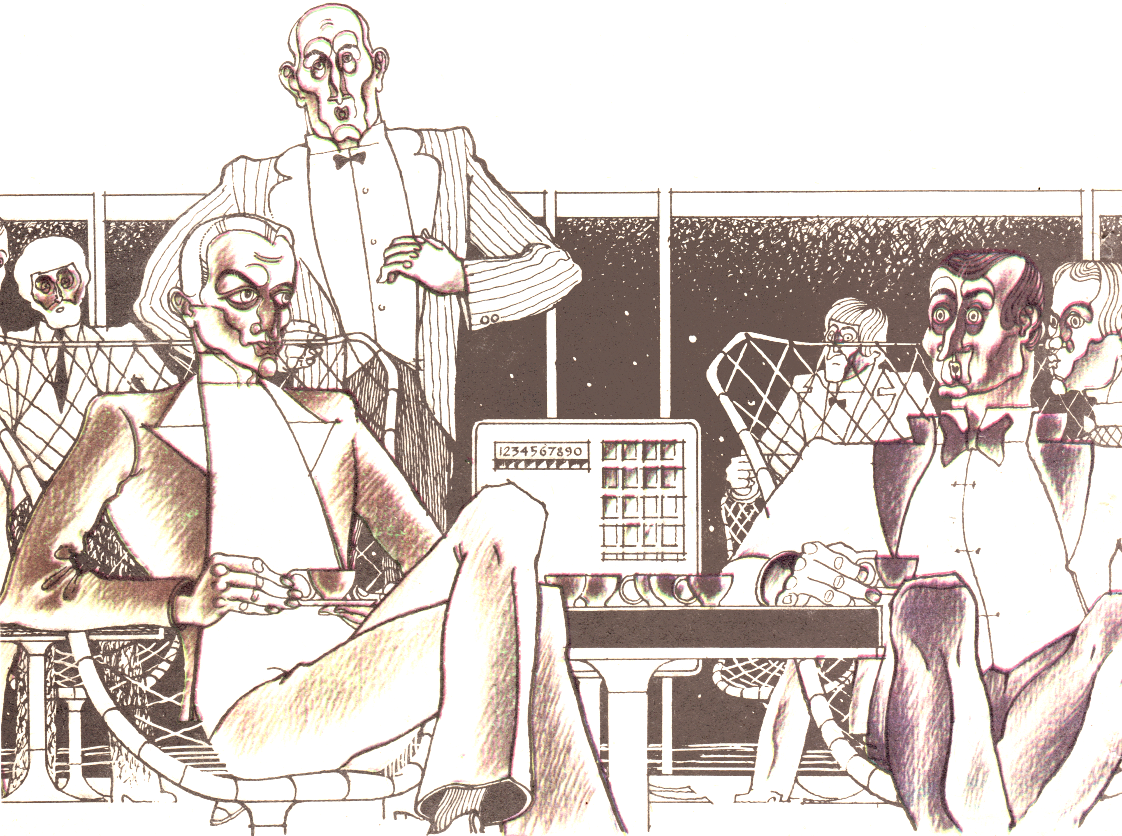
\includegraphics[width=\textwidth]{way_to_the_earth}
\caption{Рис. Евгения КАТЫШЕВА}
\end{figure}

Прослушивая старые магнитофонные записи с рассказами «человека из будущего» (см. «ТМ» № 6 за этот год), мы наткнулись на одну любопытную историю, начало которой в обработке Михаила Пухова и предлагаем вашему вниманию. Напоминаем: публикуемые под нашей рубрикой тексты адресованы в первую очередь тем, кто внимательно изучил материалы раздела «Для всех профессий» и умеет обращаться с программируемыми микрокалькуляторами «Электроника БЗ-34», «Электроника МК-54», «Электроника МК-56».

\textit{В решете они в море ушли, в решете,}

\textit{В решете по крутым волнам...}

\textit{ЭДВАРД ЛИР}

\subsection{ЧЕЛОВЕКА ВИДНО ПО ПОХОДКЕ}

Самое увлекательное приключение XXI века, как его назвали телекомментаторы, началось с чашки кофе.

Мы с Эдиком Рыжковским, парнем неплохим, но иногда до болезненности самолюбивым, завтракали в буфете астровокзала на девятом этаже. Лучший лунный кофе делают именно здесь, хотя получить его не так просто. Эдик только что совершил неслыханное — выиграл у автомата сразу две чашки, и завсегдатаи — а среди них порядочно космонавтов — поглядывали на него с уважением. Эти-то две чашки мы и смаковали, когда в помещении появился незнакомый нам человек.

Он вошел уверенной лунной походкой, какая замечается лишь у коренных «селенитов», как мы их между собой называем. На Луне все ходят замедленно — сказывается меньшая тяжесть, но у тех, кто недавно прилетел с Земли или даже Марса, это выглядит неуклюже. А человек, долгое время проживший на Луне, идет хоть и медленно, но с каким- то особым изяществом. Особенно красиво это получается у женщин.

Вот и наш незнакомец шагал именно такой, настоящей лунной походкой. Это было странно — мы хорошо знаем всех местных жителей, не так уж нас много А внешность у него была запоминающаяся — подтянутый, среднего роста глаза голубые, на голове короткий ежик совершенно седых волос. Без очков. Он направился прямо к стойке, взял не сколько бутербродов и высокий стакан оранджа, окинул взглядом зал, подошел к нашему столику и попросил разрешения сесть. Отхлебнув оранджа, повел носом — в воздухе плавал аромат нашего с Эдиком кофе.

— Вы с какой-нибудь дальней базы? — спросил Эдик.

— С дальней? — Незнакомец прищурился.— Можно сказать и так. А почему вы решили?

— Селенита видно по походке,— объяснил Эдик.— В Центре мы вас раньше не встречали, да и во всех ближних точках я тоже бывал.

— Понял вашу логику,— кивнул незнакомец.— Но скажите, где вы добыли кофе? Я видел там только это,— он поднял свой бокал,— и минеральную воду.

— Кофе в автомате.— Эдик махнул рукой в дальний конец зала.— Одна попытка в день. Только не выиграешь. Раздобыть сразу две чашки выпадает раз в жизни.

— Он только что это сделал,— добавил я.— А вот я, к сожалению, ни разу не взял ни одной.

— А что у них за игра? Шахматы? Или какой-нибудь «стартрек»?

— Нет, здесь игра для профессионалов, чтобы кофе шел в основном летному составу, а не всяким там посторонним. Садишься за штурвал воображаемого космолета и определяешь гравитацию незнакомой тебе планеты. Ее автомат подбирает случайным образом.

Незнакомец посмотрел на Эдика с недоумением.

— Что же здесь сложного? Подобрать режим, зависнуть — и все дела. До любого десятичного знака.

— Вы так считаете? — произнес Эдик слегка оскорбленно.— Топлива-то компьютер дает в обрез, только на взлет да посадку плюс еще десять секунд. И всякие ограничения. Кончилось топливо — сообщает, что ты грохнулся и не кофе тебе нужен, а квалифицированная медицинская помощь. Превысил три «же» — сообщает, что ты без сознания. Тоже, как правило, грохаешься...

— А если после взлета выключить движок на секунду-другую? — предложил незнакомец.— Потом разделить разность скоростей на время, вот и вся хитрость.

— Их не перехитришь! — хмыкнул Эдик.— Выключить двигатель, как же! Так бы всякий определил. Но выключать запрещено правилами. Поверьте выиграть почти невозможно. Я не космонавт, но на ракетах летаю много. Тем не менее сегодня мне просто повезло.

— Ты, Эдик, скромничаешь,— сказал я.— Ты в этом деле ас. А вот я управлял ракетой один-единственный раз в жизни.

— Первый раз вижу такого человека,— задумчиво проговорил незнакомец.— Видимо, дают по чашке за каждый угаданный знак?

— Точно.

— Надо попробовать.— Он встал со своего места.— Вам принести?

— Я, право, не знаю...— заколебался я.

— Несите,— сказал Эдик. В голосе его звучало сдержанное злорадство.— И лучше по две — нет, по три чашки. Но запомните — я вас предупреждал. Вы кто по специальности? Конечно, пилот?

— Бывший,— помолчав, сказал незнакомец. И пошел в дальний конец зала.

— Пижон,— сказал Эдик.— Но я его прищемил. Думает, раз он профессионал, все получится. Как бы не так! Я неоднократно наблюдал, как настоящие пилоты, даже не бывшие, возвращались ни с чем.

— Зачем ты так? Ты же его не знаешь.

— Человека видно по походке,— произнес Эдик.— Обыкновенный пижон...

Он замолчал, потому что по залу пронесся восхищенный ропот. Наш новый знакомый возвращался, балансируя подносом, уставленным чашками кофе. Как и полагается бывалому селениту, времени не терял: на ходу отхлебывал ароматный напиток. Завсегдатаи вытаращили глаза — ни один из них не видел ничего подобного.

— Себе я взял две, если не возражаете,— сказал он, опускаясь в кресло.— А вам по три, как и просили.

— Восемь знаков??? — с трудом выдавил Эдик и на длительное время потерял способность что-либо спрашивать. Он, только что герой дня, был попросту уничтожен.

— Но как вы все-таки это сделали? — поинтересовался я, немного опомнившись.— Или это секрет?

— Никаких секретов.— Он отставил пустую чашку.— Я терпеть не могу компьютеров, особенно тех, которые что-то мне запрещают. Он думает, что если запретил мне выключать движок, то я так и послушался!

— Но если его выключить, загорится транспарант «Нарушение правил» и вы лишитесь права на игру.

— Что же я, идиот? Я сделал так, чтобы он сам его выключил!

— Каким образом?

— Проще простого,— улыбнулся он.— Во время полета превысил допустимое ускорение, он выбросил транспарант «Пилот без сознания» и выключил двигатель.

— Но вы бы разбились!

— Зачем же? Я превысил ускорение на самую малость. Дал такую тягу, чтобы движок вырубился всего на пару секунд. Упасть я просто не успел. А чтобы увеличение тяги не повлияло на скорость, я дал очень малый расход, но за ничтожное время. Ускорение получилось большое, и этот электронный болван выбросил свой транспарант. Я подождал, пока он погас, разделил разность скоростей на время свободного падения, и вот результат.

Эдик сидел, опустив глаза. Лицо у него полыхало. Он, обжигаясь, пил кофе большими глотками.

— А где вы раньше летали? — спросил я чуть погодя.

— Юпитер,— сказал он.— Ио, Европа, Каллисто... Действительно, тяжесть как на Луне, вот вы и приняли меня за местного. А сейчас в отставке... По возрасту.

— И что теперь?

— На Землю,— сказал он.

— Вот и отлично,— сказал я.— Давайте полетим вместе. Я тоже туда собираюсь. В отпуск.

— По рукам. Вы мне нравитесь. Пойдете со мной штурманом? Меня зовут Михаил Коршунов. Профессиональная кличка Лунный Коршун. Не слышали? Луны Юпитера. Так договорились — летим вместе?

— Договорились,— сказал я.— Меня зовут Александр. Александр Перепелкин. Без клички. Только лайнер ушел вчера. Теперь две недели ждать.

— Лайнер? — поморщился он.— Я летел Юпитер — Луна на лайнере. Скукотища. Стюардесса разносит конфеты и воду. Заставляют сидеть в кресле... Нет, мне лайнер не по душе.

— А как же иначе? Космический лифт пока не построили.

— Вот я и думаю,— сказал Михаил Коршунов.— Простите, Эдуард, если не ошибаюсь? Вы говорили, что много ле тали на ракетах. Не знаете, где можно раздобыть корабль, хотя бы плохонький?

Эдик поднял лицо. Краска с него уже схлынула, а в глазах появилось выражение, которое мне не очень понравилось. У него такое бывает. Что-то нехорошее, мстительное.

— Плохонький? — повторил он.

— Меня устроит любой.

— Тогда я вам помогу. У меня есть именно то, что вам нужно.

Так сказал Эдик. Я-то знал, что у него нет ничего, кроме старого лунолета, вроде того, на каком мы с сыном совершили свое невероятное путешествие.

— Если движок цел,— сказал Коршунов,— беру не глядя.

— Договорились? — пародируя его интонацию, переспросил Эдик Рыжковский.

— Конечно. Я своего слова назад не беру. Никогда. У вас есть описание?

— Естественно,— зловеще усмехнулся Эдик. И выложил на стол паспорт — да-да, того самого лунолета!

Коршунов погрузился в чтение. Он шевелил губами, иногда повторяя вслух: сухая масса — две тонны. Топливо — керосин и кислород. Предназначен для перелетов вдоль поверхности Луны на расстояния не свыше 1000 километров...

И вдруг захохотал. Он смеялся долго и искренне. Эдик тоже засмеялся — сначала робко, потом все уверенней. За унижение он отомстил, счет стал один — один, и на душе у него, видимо, полегчало. На них оглядывались. Я молча ждал, пытаясь сообразить, во что может вылиться эта ситуация.

— Ну и колымага! — отсмеявшись, сказал Коршунов.— Но зачем все эти дурацкие ограничители? На ускорения, на расход, на время маневра? Учтите — я все это выброшу.

Лицо у Эдика Рыжковского стало растерянным.

— Да вы что... берете?

— Конечно. Мы же с вами договорились. Разве не так?

— Но я же просто пошутил! — воскликнул Эдик.— Прошу вас меня извинить...

— Извинения не принимаются,— холодно заявил Лунный Коршун, и вдруг стало ясно, почему его так прозвали.— Я беру ваше судно.

— И вы действительно... полетите?..

— Разумеется.

— Но это безумие! — рассвирепел Эдик.— Эта машина никогда не поднималась даже на орбиту! Она предназначена для горизонтальных полетов! Идти на ней в космос — это... это...

— Ну,— прищурился Коршунов,— смелее.

— Это то же самое, что переплывать океан на плоту! — выпалил Эдик Рыжковский.— Безумие, тысячу раз безумие!

— Но ведь переплывали же,— спокойно возразил Коршунов.— В чем только не переплывали. Интересное, легендарное было время — двадцатый век... И спасибо за хорошую мысль. Как называется ваше судно?

— Никак. Есть только номер.

— Вот и отлично. Тогда с вашего разрешения, я нарекаю его «Кон-Тики». Не возражаете?

Возражений не последовало. Коршунов встал.

— Смотреть будем завтра. Встречаемся здесь в это же время.— Он повернулся ко мне: — Договорились?

Я неуверенно пожал плечами:

— Ну, мне-то, наверное, необязательно.

— Вообще-то желательно. Принято, что при первом осмотре присутствует весь экипаж. Ведь мы идем вместе, мы же договорились. Вы мой штурман, еще не забыли?

Он взглянул на меня в упор. Никакой насмешки в его холодных глазах не было. По-моему, я побледнел. Сказать ничего не смог, только кивнул.

— Так что завтра на этом же месте,— сказал Лунный Коршун. Потом повернулся к нам спиной и своей лунной — нет, каллистянской походкой зашагал к выходу.

— Я просто хотел пошутить,— несвязно бормотал Эдик Рыжковский.— Просто пошутить. Просто-напросто пошутить...

Записал Михаил ПУХОВ

\subsubsection{МЯГКОЙ ПОСАДКИ!}

ВНИМАНИЕ!!!

Всем, кто жаждет на собственном опыте испытать радость взлета и восторг освобождения от уз гравитации;
ощутить холодное дыхание лунных скал, проносящихся на расстоянии вытянутой руки;
почувствовать, как бесплотный, казалось бы, воздух становится при входе в атмосферу грозной тормозящей средой;
познать удивительный мир орбитальных станций — царство центробежных и кориолисовых сил;
научиться ценить каждую долю секунды и каждую каплю топлива;

ВСЕМ, КТО ХОЧЕТ ПРИОБРЕСТИ НОВЫЕ ЗНАНИЯ И НАУЧИТЬСЯ ПРИМЕНЯТЬ ИХ НА ПРАКТИКЕ;
короче, ВСЕМ, КТО НАМЕРЕН ПРИНЯТЬ УЧАСТИЕ В САМОМ УВЛЕКАТЕЛЬНОМ ПРИКЛЮЧЕНИИ XXI ВЕКА — перелете с Луны на Землю на не приспособленном для межпланетных путешествий крохотном лунолете «Кон-Тики»,— МЫ НАСТОЯТЕЛЬНО РЕКОМЕНДУЕМ:

\begin{enumerate}
\item	срочно обзавестись программируемым микрокалькулятором «Электроника БЗ-34» или «Электроника МК-54»;
\item	внимательно изучить статьи, опубликованные в разделе «Для всех профессий» («ТМ № 1-4, 6 за этот год);
\item	пройти курс предварительного обучения пилотажу на программах «Лунолет-1» («ТМ», № 6-7 за этот год) и «Лунолет-2» (см. ниже).
\end{enumerate}

ВРЕМЕНИ ПОЧТИ НЕ ОСТАЛОСЬ!!! Экипаж «Кон-Тики» полным ходом ведет подготовку к старту. ТОРОПИТЕСЬ!

РЕДАКЦИЯ ЧЕСТНО ПРЕДУПРЕЖДАЕТ:

полной уверенности в благополучном исходе рискованного предприятия у нас нет. Не исключено, что нам с вами придется выпутываться из создавшейся ситуации, положившись исключительно на собственные силы. Мы должны встретить грядущие испытания во всеоружии.

Для практической подготовки к опасному перелету предлагаем вашему вниманию учебно-игровую программу «Лунолет-2».

00. ИПА 01. Fx<0 02. 14 03. 2 04. X 05. ПП 06. 82 07. Fx$^{2}$ 08. + 09. F√ 10. ИПВ 11.— 12. БП 13. 78 14. Fx≠0 15. 31 16. 0 17. ИПЗ 18. ИП7 19. -
20. 	Fx<0 21. 26 22. ИПД 23. Fx!=0 24. 30 25. ИП6 26.ИП9 27. С/П 28. БП 29. 33 30. ИПА 31 С/П 32. П1 33. \FO
34. 	П2 35. ÷ 36. П8 37. ИП5 38. ИПД 39. + 40. ÷ 41. ИП6 42. X 43. П3 44. ИПС 45. ИП3 46. ИП1 47. Fsin 48.Х 49. ИП2 50. X 51. ИП0 52. + 53. П0 54. ПП 55. 91 56. — 57. ПС 58. ИП2 59. /—/ 60. ПП 61. 82 62. + 63. ПВ 64. ПП 65. 91 66. ИПА 67. + 68. ПА 69. ИПД 70. ИП8 71. ИП2 72. X 73. -
74. 	ПД 75. Fx<0 76. 00 77. ИП8 78. ÷ 79. П2 80. БП 81. 44 82. ИП4 83. ИП3 84. ИП1 85. Fcos 86. X 87. - 88. X 89. ИПВ 90. В/О 91. FBx 92. + 93. 2
94. 	÷ 95. ИП2 96. X 97. В/О

Программа «Лунолет-2» предназначена для численного моделирования произвольных маневров космических аппаратов в непосредственной близости безатмосферных небесных тел. (Напомним, что программа «Лунолет-1» даже в варианте с постоянной горизонтальной скоростью позволяла рассчитывать лишь вертикальный маневр.) Тем не менее у обеих программ много общего. Комплект исходных данных формируется и вводится точно так же, как и в программе «Лунолет-1» в варианте с постоянной горизонтальной скоростью. Напомним: аварийный сигнал засылается в регистр 9, ускорение свободного падения на поверхности планеты в м/с$^{2}$ — в регистр 4, масса корабля без топлива в кг — в регистр 5, скорость истечения продуктов сгорания в м/с — в регистр 6, предельное ускорение, которое могут выдержать космонавты, не теряя сознания, в м/с$^{2}$— в регистр 7, начальная высота в м — в регистр А, начальная вертикальная скорость в м/с (положительным считается направление вверх) — в регистр В, начальная горизонтальная скорость в м/с (положительным считается направление к цели) — в регистр 0, расстояние до цели в м — в регистр С, запас топлива в кг — в регистр Д. Все исходные данные засылаются в произвольном порядке. После ввода полного комплекта нужно нажать В/О и С/П. Каждый ход, как и прежде, можно подразделить на два этапа — анализ ситуации и ввод исходных данных для очередного маневра.

Анализ ситуации производится аналогично тому, как это делалось в программе «Лунолет-1», только в регистре У хранится теперь не вертикальная скорость, а текущий запас топлива (лишь после самого первого останова здесь оказывается последнее число из введенного комплекта исходных данных). При останове на индикаторе светится текущая высота полета, она же хранится и в регистре А. Остальные важные параметры — вертикальная скорость, расстояние до цели, горизонтальная скорость — находятся в регистрах В, С и 0 и вызываются на индикатор командами ИПВ, ИПС и ИП0 соответственно.

Режим двигателя при маневре определяется расходом топлива, временем, за которое этот расход произведен, углом отклонения вектора тяги от вертикали (см. рисунок) и задается командой: (расход, кг) ↑ (время, с) ↑ (угол, градусы) С/П. Переключатель Р-Г при работе с программой «Лунолет-2» должен быть установлен в положение Г (градусы). Задавать время маневра равным нулю нельзя. Если вы ошибетесь, на индикаторе загорится сообщение ЕГГОГ. В этом случае нужно возвратиться на прежнюю высоту с помощью команды В/О С/П.

Аварийные ситуации, возникающие при работе с программой «Лунолет-2», и правила поведения в этих ситуациях полностью аналогичны тем, с которыми вы имели дело, когда осваивали предыдущую программу. Появление на экране нуля, как и прежде, означает контакт с поверхностью, только теперь для оценки качества посадки нужно учитывать не только вертикальную, но и горизонтальную скорость. Переход к новому варианту происходит точно так же, как и в программе «Лунолет-1».

ВНИМАНИЕ: наши игровые программы реализуют процесс численного интегрирования дифференциальных уравнений механики, и это накладывает определенные ограничения на вводимые в ходе маневра параметры. Так, при работе с программами «Лунолет-1» и «Лунолет-2» расход топлива за маневр не должен превышать 5\% полной массы ракеты (для кораблей класса «Кон-Тики» это составляет около 100 кг).

ЗАПОМНИТЕ: космонавт должен всегда быть в форме. Без постоянных тренировок нечего и мечтать о настоящих полетах — а уже в следующем выпуске «Кон-Тики» отправится в опасный рейс через океан пустоты. Для оценки степени подготовленности читательских экипажей мы будем на каждом этапе предлагать вам контрольное задание.

\subsubsection{ЗАДАНИЕ ПЕРВОГО ЭТАПА}
\begin{enumerate}
\item Какими физическими соображениями можно объяснить утверждение А. Перепелкина, что «на Луне все ходят замедленно — сказывается меньшая сила тяжести»? Есть ли в распоряжении ученых экспериментальные данные по этому вопросу?
\item Программа «Лунолет-1», игра «Угадай тяготение» (см. «ТМ» № 7). Ускорение силы тяжести 1,2345 м/с$^{2}$, запас топлива 50 кг, остальные исходные данные как в «ТМ» № 6. Экспериментально определить ускорение силы тяжести способом зависания и по методу Лунного Коршуна.
\item Программа «Лунолет-2». Запас топлива 1000 кг, расстояние до цели 250 км, начальная горизонтальная скорость равна нулю, остальные исходные данные как в № 6. Выполнить перелет и совершить посадку с минимальной скоростью и минимальным отклонением от намеченной точки.
\end{enumerate}

Ваши ответы и варианты (последовательности команд) присылайте в редакцию с пометкой «Путь к Земле». Срок отсылки — один месяц (до выхода в свет очередного номера). За правильные ответы будут начисляться очки. Победители будут выявлены, естественно, по окончании перелета.

До встречи в следующем выпуске!

\begin{figure}[H]
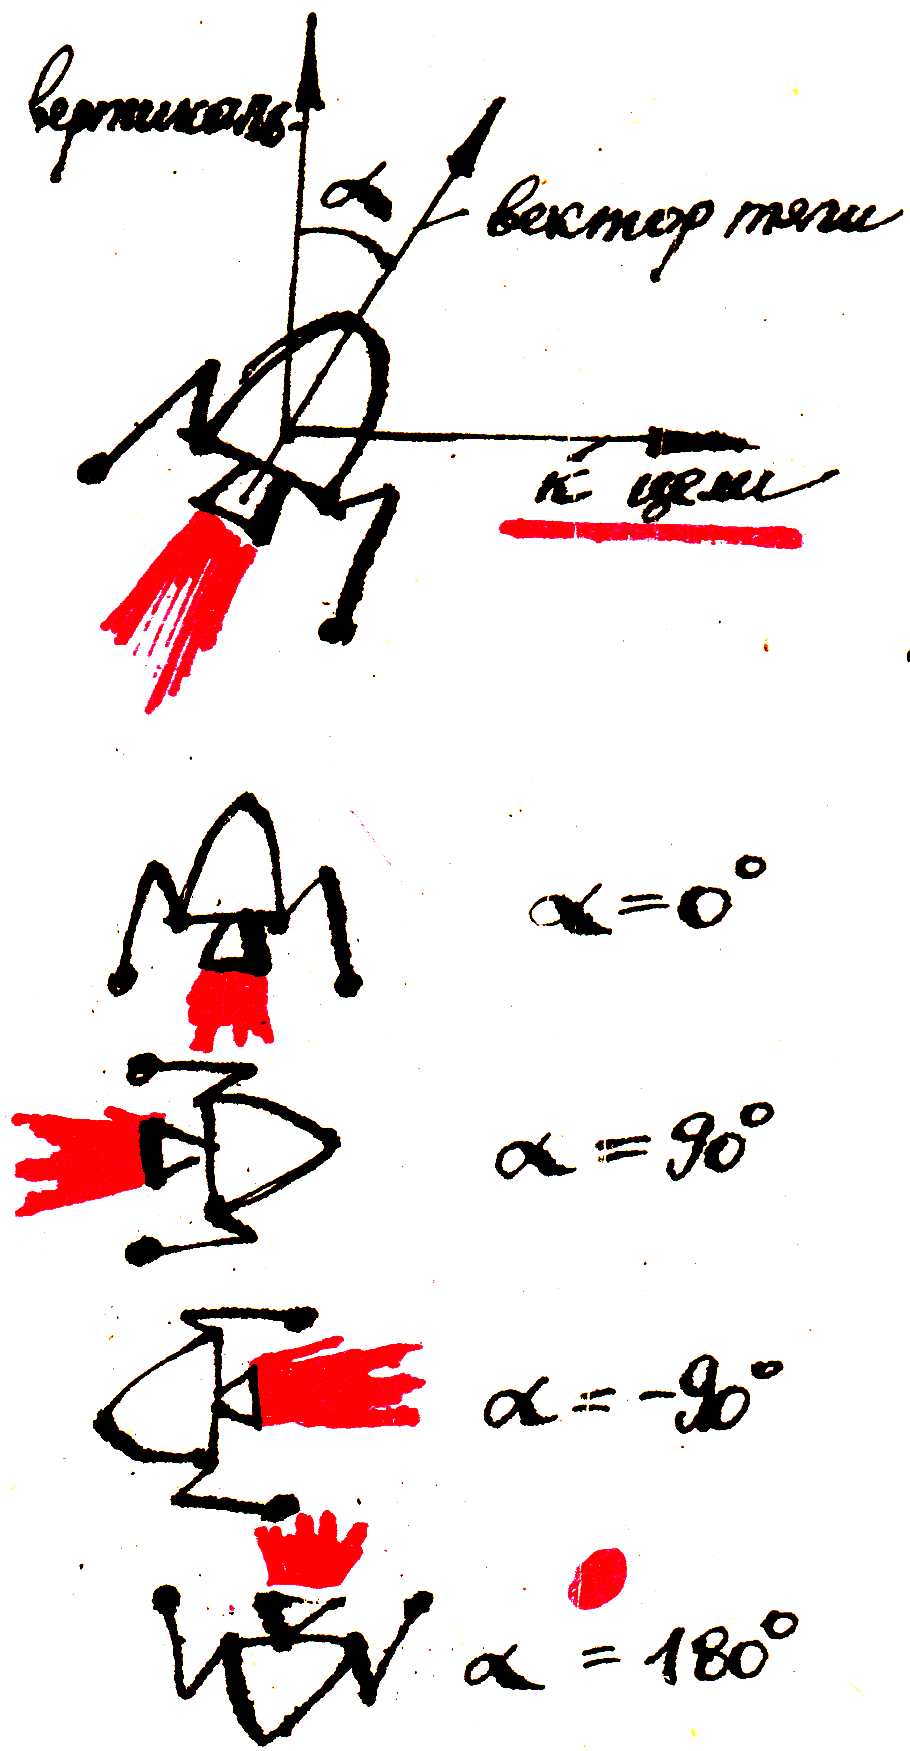
\includegraphics[width=0.25\textwidth]{lunolet2_angle}
\caption{Угол отклонения вектора тяги от вертикали задается так. О соответствует направлению «вверх», 90 — «вперед»,-90 — «назад», 180—«вниз».}
\end{figure}

\subsubsection{ДВОЕ НА БОЛИВАРЕ}
\begin{figure}[H]
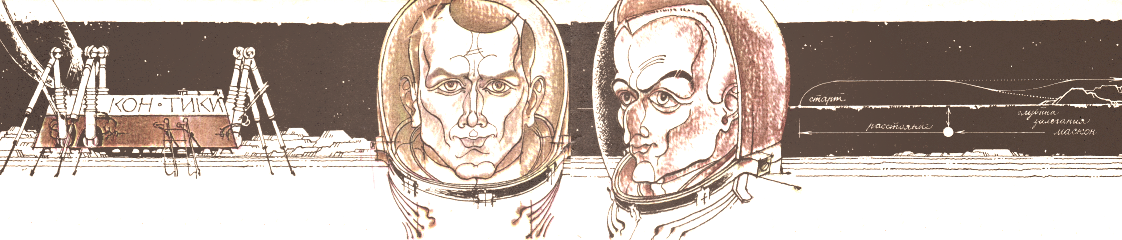
\includegraphics[width=\textwidth]{bolivar}
\caption{Рис. Евгения КАТЫШЕВА}
\end{figure}

ПРОДОЛЖАЕМ ПУБЛИКАЦИЮ ДОКУМЕНТАЛЬНО-ФАНТАСТИЧЕСКОГО ОТЧЕТА О РЕЙСЕ КРОШЕЧНОГО ЛУНОЛЕТА «КОН-ТИКИ» ПО ТРАССЕ ЛУНА—ЗЕМЛЯ, ЗАПИСАННОГО СО СЛОВ УЧАСТНИКА ПЕРЕЛЕТА А. ПЕРЕПЕЛКИНА. (НАЧАЛО СМ. «ТМ» № 8 ЗА ЭТОТ ГОД.)

— В чем дело, штурман?— крикнул вдруг Коршунов.

С момента старта прошло уже почти полчаса, постройки Центра давно скрылись из виду. Под нами тянулись однообразные безжизненные ландшафты. «Кон-Тики» мчался по низкой орбите, на высоте не более четырех километров. Облачный серп Земли и маленький рядом с ним ослепительный диск Солнца уже переместились из зенита, где они стояли в момент старта, к самому горизонту. На разгон до орбитальной скорости у Коршунова ушло около минуты: щадя меня, он избегал чрезмерных перегрузок. Лунолет он вел уверенно и спокойно — сказались четыре дня довольно изнурительных тренировочных полетов. «Чтобы почувствовать машину,— объяснил он их назначение.— И эту луну. У каждой машины свой темперамент, у каждой луны тоже. Они как женщины, штурман. Тут нужен опыт, никакая теория не поможет».

Сначала я думал, что мои штурманские обязанности будут, если можно так выразиться, чисто номинальными. В крайнем случае придется работать с киберштурманом, а я хорошо знаю эту аппаратуру. Но я ошибся. Все вычислительное и навигационное оборудование Коршунов попросту выбросил. «Не заблудимся,— объяснил он.— Опыт и здравый смысл — больше нам ничего не требуется. Лучше определять координаты на глаз, чем таскать лишний балласт на своем горбу, а потом гробануться на финише». В результате лунолет облегчился килограммов на пять- десять; из всей навигационной аппаратуры Коршунов оставил только бинокль, да и то лишь потому, что к хорошим биноклям у него слабость. Так он сказал. А мне, вместо того чтобы спокойно работать за дисплеем киберштурмана, пришлось срочно обзаводиться ветхой лоцией и комплектом пожелтевших крупномасштабных карт, а потом аккуратно разрисовывать их короткими и длинными линиями — трассами наших полетов — с обязательным указанием контрольных высот. Маршрут выбирал я — Коршунову было все равно, куда лететь. На двухминутную работу при такой организации труда уходило не меньше часа. «Я дисплеям не верю,— говорил Коршунов.— Он за секунду выдаст тебе точный разрез, но забудет сообщить, что справа от трассы вершина, а тебя каким-нибудь солнечным ветром обязательно вынесет прямо на нее, и будь здоров. Рельеф — наш главный враг, штурман. Лучшие луны те, на которых рельефа нет. Европа или, скажем, Плутон».— «Какая же это луна?— удивлялся я.— Нас учили, что это планета».— «Бывшая луна Нептуна,— объяснял Коршунов.— И вообще это как должность и звание. Луна, занимающая планетную должность. Ты еще Цереру обзови полноценной планетой. Или какую-нибудь Палладу...»

Топлива в баках «Кон-Тики» умещалось три с половиной тонны, но в предварительные полеты мы брали одну, максимум полторы. «Таскать на горбу балласт я не намерен,— сказал Коршунов.— Топлива в рейсе должно быть ровно столько, сколько необходимо. И запомни, штурман: никаких заначек. Здесь тебе не авиация. Я обязан в каждый момент точно знать, сколько у меня топлива. Знать с точностью до грамма».

На сегодняшнем старте баки — впервые за неделю — были полны. Центр Королева расположен в Центральном Заливе, и прямо над нашими головами, за прозрачным колпаком кабины, висела Земля. Обычно она выглядит огромной, но в предстартовые мгновения показалась мне весьма и весьма маленькой. Коршунов подтвердил класс: когда исчез вес, а двигатель умолк, на указателе вертикальной скорости воцарился нуль. Мы неслись по низкой круговой орбите, над незримой границей между Океаном Бурь и Морем Дождей. В стороне остались крупные кратеры Коперник и Аристарх. На маршруте не было особых препятствий — лишь один довольно протяженный горный массив на обратной стороне, с высотами, не превышающими трех с половиной километров. Поэтому Коршунов отказался подниматься выше четырех: «Я не собираюсь терять при спуске драгоценные килограммы только из- за того, что кому-то захотелось поближе к небу. Я не альпинист, а космонавт. Если бы было можно, я бы никогда не забирался выше ста метров. Так летают над Европой. Там только лед, гладкий лед, и очень редко торосы».

Вот так мы и летели: на табло нули, однообразный ландшафт усыплял, и вдруг...

— Спишь, штурман?!— заорал Коршунов. Мы сидели с откинутыми шлемами, от его крика буквально содрогнулась кабина.

Я, видимо, действительно задремал — устал за последние дни,— но от этого вопля всякий сон, конечно, пропал. Уставился в пульт, однако ничего катастрофического не обнаружил. Практически те же цифры, что и полчаса назад, светились на индикаторах альтиметра и измерителей скорости. Лишь точка, отмечавшая наше положение на лунном диске, сместилась к самому его краю. Но чтобы удостовериться, что это на самом деле так, необязательно смотреть на приборы: Земля уже заходила за горизонт.

— По-моему, все нормально,— сказал я, впрочем, не слишком уверенно.

— Вот как?— В его голосе появилась веселая злость.— Значит, штурман считает нормальным, когда корабль падает?

Я посмотрел, куда он показывал,— на индикатор вертикальной скорости. Вместо нуля, каковой красовался там совсем недавно, сейчас здесь светилось какое-то число, только весьма и весьма малое. Мы действительно «падали», но со скоростью несчастных сантиметров тридцать в секунду!

Конечно, это меня огорчило. Пусть я не профессионал, но значит ли это, что надо мной можно вот так подшучивать?

— Кошмар!— сказал я спокойно, но вместе с тем и слегка озабоченно.— И правда падаем! Если так пойдет дальше, то от нас ничего не останется... витка через полтора.

И я ему подмигнул: мол, вас понял, и нечего меня разыгрывать. Нынешний рейс Коршунов рассматривал как генеральную репетицию. Облет Луны с посадкой в точке старта. Лунолеты типа «Кон-Тики» еще никогда не выполняли подобных рейсов, никто и не подозревал, что они на такое способны. Четверть витка мы уже прошли — осталось три четверти. Три четверти, но никак не полтора.

В его холодных глазах не появилось и тени улыбки — лицо было таким же, как много часов назад, когда Эдик Рыжковский бормотал: «Я просто хотел пошутить».

— Смотри лучше, штурман,— сказал он.

Я последовал его совету. И вдруг понял. Число на указателе скорости не оставалось постоянным. Оно медленно росло — разумеется, с отрицательным знаком. На нас, стало быть, действовала неучтенная слабая сила...

— Что это значит?— озадаченно спросил я.

— Что значит?— повторил он. И вдруг опять закричал:— Я впервые на этой луне, как я могу знать? Я уже спрашивал, штурман, и спрашиваю еще раз: какие есть препятствия на выбранном вами маршруте?

Я посмотрел на карту.

— Их нет. Отклонения рельефа от условного нуля не превышают одного-двух километров. Лишь на обратной стороне мы пройдем над протяженным горным массивом с максимальными высотами около трех с половиной километров...

— Что мне та сторона?— крикнул он.— Мы еще пока что над этой, и нас тянет вниз. Что у тебя здесь, штурман? — Он ткнул пальцем в карту. И, надо сказать, именно туда, куда следовало. Все сразу стало понятно.

— Маскон!— обрадовался я.— Локальный концентрат массы! Он-то и тянет нас вниз.

— Отлично,— кивнул Коршунов.— Даже превосходно. Почему же, докладывая обстановку; вы не упомянули об этом масконе?

— А что он может?— пожал я плечами.— Гравитационная аномалия в эпицентре не превышает одного процента. Так записано в лоции. Один процент и без того слабого лунного тяготения! Ну, подпортит немножко орбиту. Но мы над ним быстро пройдем, потом она восстановится. Поле-то потенциальное! Пусть у меня мало опыта, но здравый смысл...

— Значит, вы полагаете, что нам ничего не грозит?

— Естественно.

— Хорошо,— сказал Коршунов.— Оставим все как есть.

На вид он полностью успокоился, но мне показалось, что это не совсем так, и я. с удвоенным вниманием следил за приборами. Судя по карте, маскон мы уже миновали, но скорость снижения продолжала расти, хотя не достигла еще и метра в секунду. Земля скрылась за горизонтом, сразу за ней — Солнце. «Кон-Тики» окутал мрак. Только небо вверху было усыпано бесчисленными немигающими звездами, а внизу звезды заслоняла Луна.

И вдруг мне стало страшно.

Мы летели все-таки на очень небольшой высоте, кто знает, что таится внизу, в этом бездонном мраке? Что, если там какая-нибудь вершина, не замеченная картографами? Или врет альтиметр? Совсем немного, на какой- нибудь километр? Кроме того, высота неуклонно падала, вертикальная скорость и не думала убывать. А мы и так опустились уже почти на полкилометра...

Я дал подсветку на карту. До опасного высокогорного района оставалось меньше тысячи Километров — минут десять полета с нашей скоростью. И тут до меня дошло, что мы уже летим ниже вершин — не воображаемых, а вполне реальных,— что, если так будет продолжаться, через десять минут мы неминуемо врежемся!...

Как ни удивительно, это открытие меня успокоило.

— Михаил!— сказал я.— Не понимаю, в чем дело, но орбита, кажется, восстанавливаться не собирается. Мы уже опустились ниже гор...

— И какие будут рекомендации, штурман?— насмешливо прищурился он в неярком свете индикаторов.— Идти вверх?

— Немедленно!

— Наконец-то разумные речи,— усмехнулся он, берясь за рычаги управления. Двигатель снова запел, но на этот раз перегрузка не ощущалась. С облегчением я следил, как скорость уменьшилась до нуля, потом изменила знак... Мы шли вверх. Маневр, надо сказать, был выполнен своевременно — прежней высоты мы достигли, если верить карте, уже в районе предгорий.

Я представил себе, как невидимые в темноте, всего в нескольких сотнях метров под нами проносятся зазубренные пики лунных гор, и мне вновь стало жутко. Вдруг альтиметр дает все-таки неверные показания?..

— Не нервничай, штурман,— услышал я голос Коршунова.— Они прямо под нами, и до них не меньше пятисот метров. Опытный пилот чувствует такие вещи. Мы чувствуем это кожей...

Я так и не знаю, правду ли он говорил или просто чтобы меня подбодрить. Через некоторое время опасный район остался позади. «Кон-Тики» уверенно приближался к месту своего назначения. Впереди наметилась извилистая огненная линия — лучи невидимого еще Солнца скользили по склонам высоких лунных цирков. Еще немного — и «Кон-Тики» вновь выйдет на освещенную сторону.

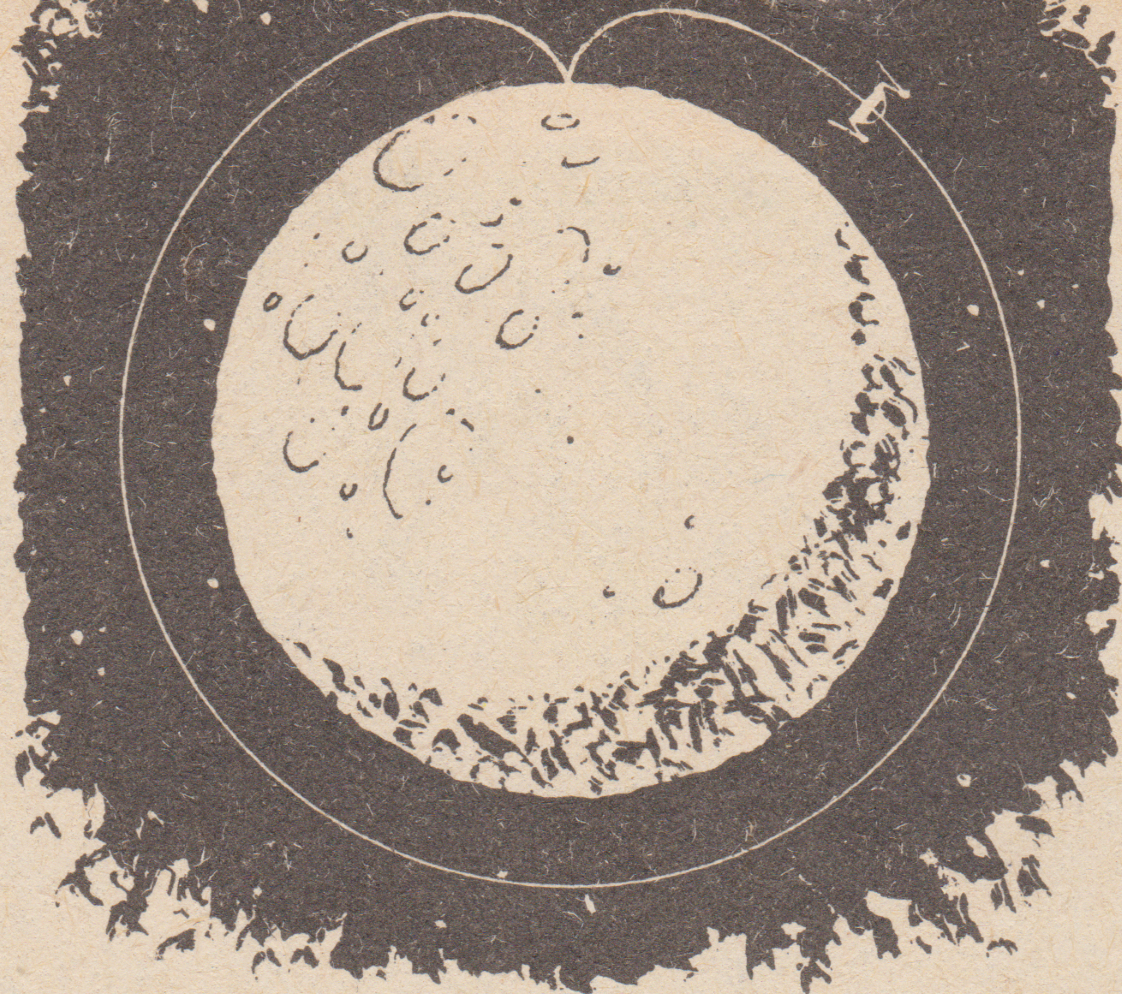
\includegraphics[width=0.25\textwidth]{bolivar2}

Мой взгляд упал на индикатор топлива. Много ли мы израсходовали на непредвиденную встречу с масконом? Вряд ли. Перегрузка почти не ощущалась...

Но я увидел такое, от чего волосы у меня на голове буквально встали дыбом.

— Михаил,— проговорил я с трудом,— посмотри сюда. Видишь?

— А в чем, собственно, дело?— поинтересовался он довольно флегматично.

— Когда мы вылетали,— сказал я, — в баках было три с половиной тонны топлива. Так?

— Да, и ни граммом меньше.

— Оказывается, мы почти все истратили,— продолжал я.— Проклятый маскон! Мы сожгли больше двух тонн! Мы не сможем теперь сесть!

— Ты в этом убежден, штурман?

— Да,— твердо сказал я.— Нам придется просить помощи. Пока не поздно. Пока мы еще на орбите!

— Чтобы я просил помощи?— бросил он яростно. И замолчал. Я следил за его лицом. На его тонких губах появилась улыбка.

— Вспомнил одну старую историю,— ответил он на мой недоуменный взгляд.— Значит, штурман, ты полагаешь, топлива на финиш не хватит?— Я молча кивнул.— Допустим, что это так. Но если бы в кабине был только один из нас, топлива бы хватило. Масса человека в скафандре — килограммов сто пятьдесят, если не ошибаюсь?

— Да,— пробормотал я, еще не понимая, куда он клонит.

— Тогда у нас остается единственный выход. Над безатмосферными лунами так иногда делают. Один из двоих идет за борт, становится спутником луны, а второй садится, заправляется, потом взлетает и подбирает товарища.

Сказать я ничего не смог. У меня пересохло во рту.

— Дальше начинается арифметика,— проговорил он жестко, и я сразу вспомнил его профессиональное прозвище.— Если за борт пойду я, ты все равно не сядешь. Погубишь и себя, и «Кон-Тики», и в конечном счете меня. Если же за борт пойдешь ты...

Он смотрел на меня холодными, немигающими глазами.

— Словом, как говорилось в той истории, Боливар не вынесет двоих. Что скажешь, штурман?..

Записал Михаил ПУХОВ

\subsubsection{мягкой ПОСАДКИ}

Как видим, экипаж «Кон-Тики» времени зря не теряет; не будем терять и мы. Совершить самостоятельный орбитальный полет вокруг Луны (или любого другого небесного тела) может каждый читатель нашего раздела. Все, что для этого требуется,— это программируемый микрокалькулятор «Электроника БЗ-34» или «Электроника МК-54» и предлагаемая вашему вниманию игровая программа «Лунолет-3».

00.ИПА 01.ПА 02.ИП7 03.— 04.Fx<0 05.12 06.ИПВ 07./—/ 08.$\div$ 09.П2 10.БП 11.36 12.ИП4 13.ИПА 14.$\div$ 15.F$\sqrt{}$
16.ИП7 17.Х 18.\XY 19.С/П 20.П9 21.П8 22.П2 23.$\div$ 24.ИПД 25.ИП8 26.— 27.Fx$\geq$0 28.00 29.ПД 30.ИП5 31.+
32.$\div$ ЗЗ.ИП6 34.Х 35.П8 36.ИП0
37.ИП8 38.ИП9 39.Fsin 40.Х 41.ИПВ
42./—/ 43.ПП 44.89 45.+ 46.П0 47.ПП 48.93 49.9 50.0 51.X 52.F$\pi$ 53.$\div$ 54.ИПА
55.$\div$ 56.ИПС 57.+ 58.ПС 59.Fcos 60.Fx<0 61.61 62.Fx$\geq$0 63.63 64.С/П 65.ИПВ 66.ИП8 67.ИП9 68.Fcos 69.X 70.ИП7 71.ИПА 72.$\div$ 73.Fx$^{2}$ 74.ИП4 75.X 76.— 77.ИП0 78.ПП 79.89 80.+ 81.ПВ 82.ПП 83.93 84.2 85.$\div$ 86.ИПА 87.+ 88.B/O 89.ИП0 90.X 91.ИПА 92.$\div$ 93.+ 94.ИП2 95.X 96.B/O

Программа «Лунолет-3» предназначена для численного моделирования различных маневров космических аппаратов, включая взлеты, посадки, выход на круговые и эллиптические орбиты вокруг безатмосферных небесных тел. В обращении она аналогична предыдущим («ТМ», № 6—8 за этот год); небольшие отличия связаны с тем, что это первая из наших собственно космических программ — она позволяет нам (с помощью ПМК) победить тяготение.

В регистры 1 и 3 вводятся наглядные видеосообщения «Корабль находится над видимой стороной луны» (Е -0) и «Корабль находится над обратной стороной луны» (Е 0-). Буква Е обозначает планету (например, Землю), 0 — луну (например, Луну с большой буквы), знак «минус» — космический корабль. (Если моделируется полет в окрестностях планеты, возможна и иная интерпретация: например, Е — звезда, 0 — планета.) Для формирования и ввода видеосообщений в память ПМК нужно выполнить следующие операции:

Сх $\div$ (ЕГГОГ) ВП ВП F10$^{x}$ ВП /—/ 12 КСх (ЕГГОГ) ВП П1

Сх $\div$ (ЕГГОГ) ВП ВП F10$^{x}$ ВП /—/ 3 КСх (ЕГГОГ) ВП ПЗ

Обе последовательности команд отдаются в автоматическом режиме, после ввода программы в ПМК. Слово в скобках означает, что в соответствующем месте на индикаторе появляется сообщение ЕГГОГ (ошибка); это естественно — все буквенные шифры формируются именно из него.

В регистры 4, 5, 6, 0, В и Д вводятся те же исходные данные, что и при работе с программами «Лунолет-1» и «Лунолет-2». Напоминаем: (ускорение свободного падения на поверхности небесного тела, м/с$^{2}$) П4 (масса корабля без топлива, кг) П5 (скорость истечения продуктов сгорания, м/с) П6 (начальная горизонтальная скорость, м/с) ПО (начальная вертикальная скорость, м/с) ПВ (запас топлива, кг) ПД. В регистр, 7 заносится радиус небесного тела в метрах (например, для Луны это реализуется командой 1738000 П7), в регистр А — начальное расстояние корабля от центра небесного тела (если он стоит на поверхности, то оно совпадает с радиусом небесного тела), в регистр С — начальное угловое расстояние корабля от центра видимой стороны луны (или дневной стороны планеты) в градусах. 0 соответствует центру видимой стороны, 90 и —90 — границам видимой и обратной сторон, 180 — центру обратной стороны. На полный оборот вокруг небесного тела, уходит, естественно, ровно 360 градусов. Переключатель Р—Г при работе с программой «Лунолет-3» должен быть установлен в положение «Г».

После ввода программы, формирования и ввода видеосообщений и комплекта исходных данных нужно нажать клавиши В/О и С/П. При останове на индикаторе светится округленная до десятых долей метра текущая высота полета. В регистре У находится очень важный для орбитальных полетов параметр — первая космическая скорость на данной высоте; она вызывается на индикатор командой \XY. Текущие значения остальных переменных — расстояние до центра небесного тела, вертикальная и горизонтальная скорости, угловое расстояние от центра видимой стороны и запас топлива — находятся в регистрах А, В, 0, С и Д и вызываются на индикатор соответственно командами ИПА, ИПВ, ИП0, ИПС и ИПД.

После анализа текущей ситуации нужно ввести исходные данные для очередного маневра. Маневр определяется теми же величинами, что и в программе «Лунолет-2», но задается несколько иной командой: (угол отклонения вектора тяги от вертикали, градусы) ПП (расход топлива, кг) ПП (время, с) С/П. Угол 0 соответствует направлению «вверх», 90—«вперед», 180—«вниз», -90 — «назад» (как и на схеме в прошлом номере «ТМ»). Если команда на двигатель подана с превышением наличного запаса топлива, она блокируется: на индикаторе загорается прежняя высота. В этом случае нужно задать маневр заново.

Для облегчения анализа ситуации в программе «Лунолет-3», помимо основного останова, предусмотрен еще и дополнительный, демонстрационный: на индикаторе при этом загорается видео- сообщение, наглядно показывающее, где находится в данный момент корабль. После появления видеосообщения нужно нажать С/П.

В нормальной ситуации основной и демонстрационный остановы чередуются; если демонстрационный останов начинает повторяться, это означает, что корабль достиг поверхности и ПМК методом последовательных приближений рассчитывает значения переменных величин в момент посадки. В этом случае следует нажимать С/П до появления на индикаторе цифры 0 (сигнал о посадке).

Если цель полета — выйти на круговую орбиту, то в ходе маневрирования нужно добиться того, чтобы горизонтальная скорость по возможности совпала с первой космической скоростью для данной высоты, а вертикальная равнялась нулю. В противном случае орбита получится эллиптической, а если она еще и пересекается с поверхностью небесного тела, то это, естественно, не приведет ни к чему хорошему.

Взлет и посадка производятся точно так же, как и при работе с программами «Лунолет-1» и «Лунолет-2». Аналогично выполняется и переход к новому варианту.

Расход топлива при маневре не должен превышать 5\% от полной массы корабля (для лунолетов класса «Кон- Тики» это составляет 100—200 кг, в зависимости от наличного запаса топлива). Не рекомендуется также задавать время маневра больше 100 с. Последнее ограничение снимается лишь в свободном полете, после выхода на орбиту; но и в этом случае следует анализировать ситуацию хотя бы каждые 1000 с.

Главные неприятности, подстерегающие космонавта при полетах на низких окололунных орбитах,— это локальные концентрации массы (масконы) и неровности рельефа. Что такое неровность рельефа, понятно — это просто гора. А вот что такое маскон?

Сразу после запуска первых искусственных спутников Луны обнаружилось, что их орбиты искажаются (причем существенно, на десятки и сотни метров) под влиянием какого-то неизвестного фактора, хотя, казалось бы, учтено было все: гравитационные возмущения от Земли, Солнца и даже... давление солнечных лучей. Причиной этих искажений оказались так называемые масконы — скрытые под поверхностью Луны скопления более плотных пород, нежели окружающие. По поводу происхождения масконов среди ученых все еще нет единого мнения; зато известно, что средний маскон проявляет себя как точечная масса, составляющая по величине $10^{-6}—10^{-5}$ массы Луны и залегающая на глубине порядка 50 км. Нетрудно прикинуть, что в эпицентре, непосредственно над масконом, возникает дополнительное гравитационное ускорение порядка нескольких миллиметров в секунду за секунду. Казалось бы, это совершенно ничтожная величина, однако, как уже отмечалось, действие масконов приводит к значительным изменениям орбит лунных спутников. Как это выглядит на практике, можно проверить экспериментально с помощью следующей программы:

00.Сх 01.ИПА 02.+ 03.ПА 04.ИП7 05.— 06.Fх<0 07.14 08.ИПВ 09./—/
10.$\div$ 11.П2 12.БП 13.31 14.С/П 15.П9 16.П8 17.П2 18.$\div$ 19.ИПД 20.ИП8 21.— 22.Fx$\geq$0 23.00 24.ПД 25.ИП5 26.+
27.$\div$ 28.ИП6 29.Х 30.П8 31.ИП8
32.ИП9 33.Fsin 34.Х 35.ИПВ 36.ПП 37.77 38.ИПС 39.Х 40.ИП3 41.$\div$ 42.+
43.— 44.ИП2 45.Х 46.ИП0 47.+ 48.П0 49.ПП 50.70 51.ИПС 52.+	53.ПС
54.ИП0 55.ПП 56.77 57.— 58.ИП4 59.— 60.ИП8 61.ИП9 62.Fcos 63.Х 64.+ 65.ИП2 66.Х 67.ИПВ 68.+ 69.ПВ
70.FBx 71.+ 72.ИП2 73.Х 74.2 75.$\div$ 76.В/О 77.ИП0 78.Х 79.ИП7 80.$\div$
81.ИПС 82. ИПЗ 83.$\div$ 84.Farctg 85.Fcos 86.Fx$^{2}$ 87.FBx 88.X 89.ИП1 90.Х 91.В/О

Пользоваться этой программой (называется она, естественно, «Маскон») не сложнее, чем программой «Лунолет-3», на базе которой она разработана. Комплект исходных данных остается примерно тем же, только вместо видеосообщений в регистры 1 и 3 нужно занести соответственно дополнительное гравитационное ускорение в эпицентре маскона в м/с$^{2}$ (например, 0,01) и глубину залегания маскона в метрах (например, 50 000). Кроме того, измерять расстояния в угловых единицах при сравнительно небольших перемещениях не очень удобно; поэтому в программе «Маскон» вместо полярной системы координат используется прямоугольная с началом в эпицентре маскона, а в регистре С откладывается горизонтальная координата корабля в метрах. Например, если он стартует в направлении маскона с расстояния 500 км, в регистре С должно размещаться число -500 000. Первая космическая скорость программой «Маскон» не рассчитывается; ее нетрудно вычислить при анализе ситуации с помощью команд ИП7 ИП4 X F$\sqrt{}$ (в отличие от «Лунолета-3» сила тяжести здесь от высоты не зависит). При приближении к маскону рекомендуется задавать время маневра не более 10 с. В остальном правила обращения с программой остаются прежними.
До сих пор мы имели дело с небесными телами, гладкими, как бильярдный шар (во всяком случае, это молчаливо подразумевалось). Для моделирования маневров космических аппаратов в сложных условиях высокогорья служит программа «Вершина»:

00.ИПА 01.Fx<0 02.16 03.$\uparrow$ 04.ИП2 05.\XY 06.$\div$ 07.Fx$^{2}$ 08.F$\sqrt{}$ 09.ПП 10.89 11.П2 12.ПП 13.33 14.Fx=0	15.03 16.С/П 17.П9 18.П8 19.П2 20.$\div$ 21.ИПД 22.ИП8 23.— 24.Fx$\geq$0 25.00
26.ПД 27.ИП5 28.+ 29.$\div$ 30.ИП6 31.X 32.П8 33.ИПС 34.ИП8 35.ИП9 36.Fsin 37.X 38.ИПВ 39.ИП0 40.X 41.ИП7
42.$\div$ 43.— 44.ИП2 45.X 46.ИП0 47.+
48.П0 49.ПП 50.86 51.+ 52.ПС 53.ИП0 54.Fx$^{2}$ 55.ИП7 56.$\div$ 57.ИП4	58.—
59.ИП8 60.ИП9 61.Fcos 62.X 63.+
64.ИП2 65.X 66.ИПВ 67.+ 68.ПВ
69.ПП 70.86 71.ИПА 72.+ 73.ПА
74.ИП3 75.ИПС 76.ИП1 77.$\div$ 78.Fx$^{2}$ 79.1 80.+ 81.$\div$ 82.— 83.ИП7 84.— 85.B/O 86.FBx 87.+ 88.ИП2 89.X 90.2
91.$\div$ 92.B/O

Правила обращения с этой программой такие же, как и с предыдущей. В регистр 3 заносится высота горы в метрах (например, 5000), в регистр 1 — полуширина горы (тоже в метрах) на высоте, вдвое меньшей. Начало координат располагается в центре основания горы, в регистре С откладывается горизонтальная координата корабля в метрах. При первом останове и в случае блокировки программы из-за перерасхода топлива на индикаторе высвечивается расстояние от центра планеты, во всех остальных ситуациях — текущая высота полета (с учетом рельефа).

С помощью программ «Лунолет-3», «Маскон» и «Вершина» вы сможете неоднократно пройти окололунным маршрутом «Кон-Тики», испытать на опыте опасности таких рейсов. Но космонавт должен быть всегда в форме — впереди нас ожидают еще более тяжелые испытания. Встретить их во всеоружии может лишь тот, кто выполнит наше очередное задание.

\begin{enumerate}
\item Программа «Лунолет-3». Повторить окололунное путешествие «Кон-Тики». Комплект исходных данных: 1,62 П4 2250 П5 3660 П6 1738000 П7 ПА 0 П0 ПВ ПС 3500 ПД. Взлететь, выйти на круговую орбиту высотой 4000 м, облететь Луну и совершить мягкую посадку в точке старта (угловое расстояние корабля от центра видимой стороны должно составлять при этом 360 градусов; ошибка всего в один градус — это примерно 30 км вдоль лунной поверхности).
\item Программа «Маскон», исходные данные: 400000 /-/ ПС 0,02 П1 50000 П3, остальные те же, что и в предыдущем случае. Стартовать, выйти на круговую орбиту высотой 3000 м, пролететь над масконом и совершить мягкую посадку в 500 км за ним.
\item Программа «Вершина», исходные данные: 400000 /—/ ПС 10000 П1 П3, остальные те же, что и в предыдущем случае. Стартовать и совершить мягкую посадку на вершине горы (в точке с горизонтальной координатой 0).
\item Прав ли был Коршунов, когда демонтировал 50 кг навигационной аппаратуры? Зачем он так поступил?
\item К какому приблизительно перерасходу топлива привела встреча «Кон-Тики» с масконом?
\item Видите ли вы какой-нибудь выход из сложившейся на «Кон-Тики» ситуации (кроме того, который предлагает Коршунов)?
\end{enumerate}

Ответы и варианты (последовательности команд) присылайте в редакцию. Срок, как обычно, один месяц.

\subsection{ПРОЩАЙСЯ С ЭТОЙ ЛУНОЙ!}
Продолжение. Начало см. «ТМ» № 8—9 за этот год.

Мы стояли рядом с «Кон-Тики» на лунных камнях. Тени прятались под ногами. Машина подтвердила, на что способна: совершив кругосветное путешествие, «Кон-Тики» вернулся на собственную стоянку, в ту же точку, откуда взлетел. Коршунов придерживался за посадочную опору, его пошатывало. Что ж, он поработал на совесть. Когда амортизаторы коснулись грунта, топлива в баках не осталось ни капли, зато и скорость ушла в ноль — и вертикальная и горизонтальная. Я, надо сказать, тоже не чувствовал себя бездельником — одних только цифр («высота... скорость... высота... скорость...») за последние минуты пришлось надиктовать сотни. Но все это было в прошлом.

А здесь, куда мы столь блистательно возвратились, все осталось как было. Все так же стояли на своих местах лунолеты, из-за близкого горизонта выступали здания промышленного блока. С момента старта минуло чуть менее двух часов, и Солнце по-прежнему висело в зените. Разве что отодвинулось от Земли на пару своих диаметров.

Коршунов наконец поднял голову.

— Вот она.— Он показал на запад. Над горизонтом поднималась блестящая вертикальная черточка.— Станция «ЮГ», «Юрий Гагарин», наша первая остановка...

«Остановка» довольно бодро взбиралась к зениту. На восхождение ей потребовалось минуты три. Теперь, наблюдаемая с торца, она выглядела уже не черточкой, а едва различимым кружочком.

— До нее всего пятьдесят километров,— сказал Коршунов,— но у нас свой отсчет, для нас это четверть дороги. Мы заправимся там и пойдем дальше. Когда старт, штурман?

Я вздрогнул.

— Ну, вроде договорились на завтра...

— Да,— подтвердил он.— Но «завтра» — понятие растяжимое. Ты штурман, назначай точное время.

— Слишком рано, может, не стоит?— полувопросительно предложил я.— Нужно хорошенько выспаться, отдохнуть... Может, часов в двенадцать?

— Договорились,— кивнул Коршунов.— Завтра, в полдень по Москве.— Он провожал взглядом упускающуюся к восточному горизонту черточку.— Мы заправимся там, штурман, наполним баки «Кон-Тики», а потом...— Он посмотрел в зенит, где громадным дымным кольцом светилась Земля.— Даже не верится... Несколько дней, и мы будем там.

— С Юпитера, наверное, она выглядит поскромнее,— сказал я.

— С Юпитера?..— повторил он, странно на меня посмотрев. И, помолчав, добавил: — Ты, Саша, видел когда- нибудь Меркурий? — В голосе его появилась горечь, будто с этой планетой были у него связаны какие-то сокровенные, причем не слишком приятные воспоминания.

— Меркурий? — сказал я, подумав.— Нет. По-моему, никогда. Да его почти никогда и не видно. Он слишком близко к Солнцу, не разглядишь.

— Правильно,— кивнул он.— Меркурий не удаляется от Солнца — от диска Солнца — больше чем на двадцать градусов, поэтому его трудно увидеть. Но знаешь ли ты, Саша,— голос его зазвенел,— знаешь ли ты, что из системы Юпитера Земля кажется вдвое ближе к Солнцу, чем Меркурий отсюда?! Вдвое, Саша! А я провел там двадцать лет. Безвылазно двадцать лет! Знаешь, сколько раз за эти годы я видел Землю? Планету, на которой родился?! Но мы там будем — я даю слово!

Он почти кричал. В глазах его была ярость.

— Но, может быть, в телескоп...— неуверенно начал я.

— В телескоп?! — Он ударил кулаком по амортизатору. «Кон-Тики» качнулся. Коршунов опустил руку и почти спокойно закончил: — Да, разве что в телескоп. В телескоп ее иногда видно.

Некоторое время мы молчали.

— Извини меня, Саша,— сказал он потом.— Со мной бывает... Особенно после трудного финиша. И еще, не обижайся на меня — ты знаешь, о чем я. Это была просто шутка.

Зря, конечно, он об этом напомнил. Обошлись бы без его извинений. А сейчас... Я вновь увидел перед собой злосчастный индикатор топлива, и у меня снова похолодела спина, как там, наверху, когда он самым серьезным тоном предложил мне идти за борт, чтобы подождать его на орбите...

— Пойми, это ракета. Эта машина, пусть она размером с автомобиль, по сути своей все же ракета, и неплохая. А любая ракета требует на финиш меньше топлива, чем было затрачено на старт. Ракете легче финишировать, чем стартовать, потому что на финише она сама легче.

Я молчал. Мне было неприятно его слушать. Напрасно он об этом заговорил.

— Опытный пилот,— продолжал он,— всегда знает, сколько топлива оставить на финиш. Меньше половины, но вполне определенную долю. Будто делишь отрезок в золотой пропорции... Не гневайся на меня, штурман, я просто пошутил, я не думал тебя обидеть.

Я упорно молчал. Станция «Юрий Гагарин» давно скрылась за горизонтом. Честно говоря, на стоянке нам совершенно нечего было делать.

— Молчишь? — сказал Михаил Коршунов.— Тогда пока. Не забудь — завтра в двенадцать ноль-ноль.

— Пока,— буркнул я, и мы вместе двинулись по тропе, по направлению к «воздушным воротам» Центра имени Королева.

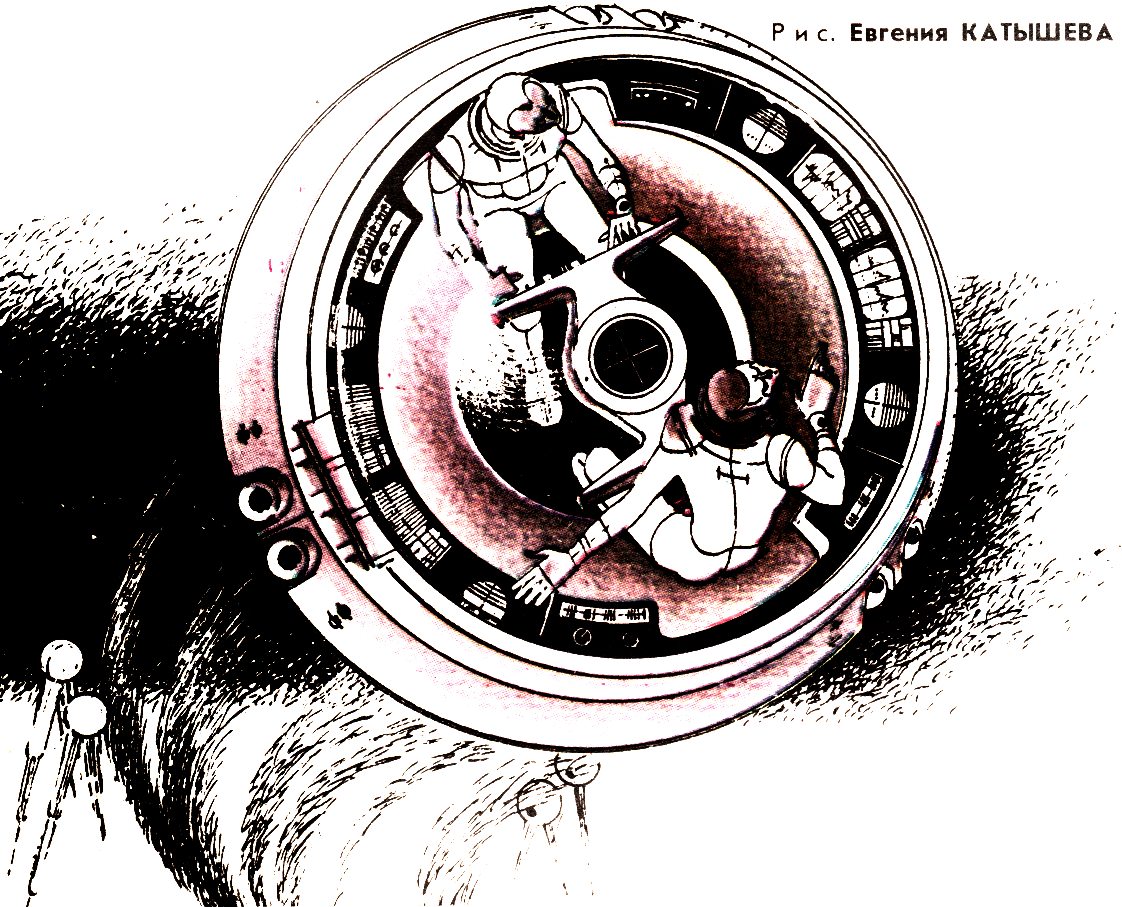
\includegraphics[width=0.25\textwidth]{start}

Назавтра я был на месте за час до намеченного срока. Отдохнуть так и не удалось. Вечером в информационной программе показывали репортаж о нашем окололунном полете. Так у нас всегда — думаешь, ты один, а за тобой следят десятки внимательных глаз. Особенно удалась оператору сцена после посадки, когда мы с Коршуновым стоим рядом с «Кон-Тики» и смотрим прямо в камеру. Репортаж делали со станции «ЮГ» — с двухсот километров взяли так, будто снимали в упор. Им что — атмосферы нет, условия идеальные... Коршунов что-то говорит, а я молчу, и физиономия у меня до удивления глупая. И текст соответствующий, юмористический. «Наш Перепелкин в когтях у Лунного Коршуна», «Перепелкин попадает в переплет»... Или «в переделку», точно не помню. Ужас! Не ровен час, увидит жена... А если еще и сын?..

Этим репортажем вчерашние неприятности не кончились. Совсем поздно приходил Эдик Рыжковский, опять клял себя, слезно отговаривал от участия в перелете. «Это безумие, чистой воды безумие! Слетать вокруг Луны может каждый, дело нехитрое. Подумаешь — взлететь, а потом сесть. А вот как вы будете выходить к станции, ты себе представляешь? В секунду она делает полтора километра, в час — шесть тысяч! Если уйдет вперед, за ней уже не угнаться! Но и это пустяк по сравнению с тем, что ждет вас потом. Даже свет летит до Земли больше секунды! Нет, ты себе представляешь, что это значит?»

И так два часа, будто не понимает — как же мне теперь отказываться? Словом, заснул под утро, встал в расстроенных чувствах. Настроение — хуже некуда. Называется, отдохнул...

Я скучал в своем кресле, верха не опускал. Ждал, что вот-вот появится Коршунов, но он, судя по всему, исповедует «вежливость королей». Обычно на стоянке бывает безлюдно, но сейчас здесь, если можно так выразиться, царило оживление. Неподалеку от «Кон- Тики» припарковался тяжелый гусеничный вездеход с крупными буквами на борту: ТВ. Два озабоченных молодых человека в скафандрах возились там со своими телекамерами. Ну, с этими-то я еще мог примириться: тут по крайней мере намерений не скрывают. Но когда за тобой подсматривают с орбиты! Стояла на краю площадки и цистерна заправщика. Как правило, они делают свое дело ночами, а днем где-то скрываются. Этот, стало быть, остался специально, задела за живое вчерашняя передача. Действительно, водитель в конце концов не выдержал, спрыгнул из кабины и подошел ко мне. Лицо у него было открытое, симпатичное.

— Вас я уже заправил,— сказал он, словно бы извиняясь.— Все полторы тонны, как и просили.

— Всего полторы?

— Как в заявке, тютелька в тютельку,— сказал он.— С точностью до грамма, фирма гарантирует. А вы правда собираетесь туда? — Он ткнул пальцем в небо.— Не страшно?

— Нет,— твердо ответил я.

— Так не хватит же,— удивился заправщик.— У нас даже до «Циолковского» все берут по две с половиной.

— Нам хватит,— успокоил я его.— Мы профессионалы, не какие-нибудь любители-селенологи.

Он понимающе кивнул и отошел. Я снова остался наедине с неприятными мыслями. Полторы тонны! Выходит, Коршунов заказал топлива только до орбиты, как всегда, в обрез. Он просто неисправим! Но, надо сказать, его уверенность успокаивала... Было уже, наверное, без пяти двенадцать, когда ребята с телевидения засуетились, наставили камеры в сторону тропинки. На вершине холма появился Коршунов. Он приближался к нам своим неторопливым каллистянским шагом.

Случайно мой рассеянный взгляд обратился к небу. И тут я увидел такое, что мгновенно забыл и о телевидении, и о Коршунове с его «королевской вежливостью»!

Над западным горизонтом медленно восходила сверкающая черточка станции «ЮГ». Значит, мы должны взлетать прямо сейчас, немедленно, чтобы успеть ее перехватить! Еще три минуты — и она пройдет над нашими головами! Гнаться за ней потом — занятие, как правильно заметил Эдик Рыжковский, вполне безнадежное. Значит, придется ждать еще два часа...

Почему же вчера, планируя сегодняшний старт, мы упустили это из виду? Ну, мне простительно, но как мог забыть Коршунов — он-то действительно профессионал!

Я снова посмотрел на него. Он шагал размеренной поступью, словно позируя телекамерам. Телевидение не зевало; чувствовалось, что в отличие от командира «Кон-Тики» этим молодым людям есть куда торопиться!

Внезапно перед моим мысленным взором встало лицо Коршунова в момент вчерашнего разговора. «Ты штурман, назначай точное время!» Неужели это новая шутка?!

Ну ладно, подумал я, посмотрим, кто будет смеяться последним. Вы изволите шутить, Лунный Коршун, пожалуйста. Не будем вам мешать в ваших невинных забавах! Взлетайте, садитесь, делайте что хотите. Вы, очевидно, рассчитываете, что штурман с исказившимся от страха лицом будет хватать вас за руки и несвязно лопотать: «Станция, станция!..» Нет уж, не будет этого! Вот если вы все-таки стартуете — в чем я сильно сомневаюсь,— тогда, быть может, штурман и намекнет тактично, что, дескать, поезд давно ушел! И, значит, пора возвращаться, иначе никакая «золотая пропорция» вам не поможет! Вот потом и позируйте перед объективами!..

Он ступил на лесенку в тот самый момент, когда «Юрий Гагарин» проходил точно над нашими головами. До телевидения, кажется, тоже дошло: одна из камер уставилась прямо в зенит. Коршунов как ни в чем не бывало занял свое место, опустил прозрачный верх. Зашипели баллоны, наполняя кабину воздухом. Через минуту он поднял забрало шлема. Я последовал его примеру. В кабине было прохладно, воздух еще хранил в себе память о своем жидком прошлом.

— Прощайся с этой луной, штурман! — произнес Коршунов, посмотрев на часы. Стрелки — а часы у него стрелочные, как у всех космонавтов,— сошлись в верхней точке циферблата.— Двенадцать ноль-ноль!..

И он нажал стартер! За прозрачным колпаком взметнулось пламя, двигатель загремел, и «Кон-Тики» ринулся в небо. Лицо у Коршунова было счастливое; неужели он ни о чем не подозревал? Мне даже стало его жалко, но что делать? Я открыл было рот — сообщить, что пора возвращаться (а «Гагарин» уже опускался к восточному горизонту), как вдруг...

«Кон-Тики» сильно тряхнуло, и, сверкая в лучах Солнца, от корабля веером полетели три трубчатые конструкции — наши посадочные опоры! Коршунов отстрелил шасси! Теперь нам оставался только один путь — вверх, на орбиту!..

— Прощайся с этой луной, штурман! — покрывая гром двигателя, прокричал Коршунов.— Эти сто килограммов больше нам не нужны! Пусть они остаются, а мы пойдем дальше!..

Он воздел руку кверху и, конечно, ушиб пальцы о крышу кабины. Сказать я ничего не мог — во всяком случае, ничего связного. Маршевый двигатель победно гремел.

— Станция... — бормотал я. — Но станция... Станция...

Перегрузка не давала мне шевельнуть даже пальцем, не то что рукой. Кажется, я пытался показывать ему глазами, но тщетно! Вертикальная черточка «Юрия Гагарина» застыла над горизонтом. Мы не набрали и половины орбитальной скорости, а станция ушла уже километров на двести и все еще удалялась!

Наконец Коршунов уловил мое беспокойство. Какое-то время он молча смотрел вперед. Конечно, он сразу все понял, но ничем не дал понять, что ситуация его встревожила.

— Держись, штурман! — прокричал он.— Обратного пути нет! Мы догоним ее, даю слово!..

Перегрузка заметно усилилась, мне стало нехорошо. Но когда двигатель умолк и мы вышли на орбиту «Гагарина», тот по-прежнему висел над горизонтом далеко впереди, а топлива в баках «Кон-Тики» оставалось всего 40 кг!

Возьми себя в руки, сказал я себе, мы на орбите, ничего страшного нам не грозит. Ну, пришлют в крайнем случае спасательный катер. И опять подстроят какую-нибудь веселенькую телепередачку...

\includegraphics[width=0.25\textwidth]{ug1}

Но Коршунова, видимо; такие проблемы не волновали. Он долго изучал станцию в свой любимый 15-кратный бинокль.

— До нее двести пятьдесят километров,— сказал он наконец, передавая бинокль мне. Выглядел «ЮГ» внушительно — этакая 600-метровая, парящая в пустоте башня, ощетинившаяся антеннами и солнечными батареями.— Идти на нее в лоб бессмысленно, не хватит никакого топлива. С десяти километров я бы еще рискнул, но не более... Постой, высота у нас пятьдесят, если не ошибаюсь?..— И вдруг он засмеялся.— Знаешь, штурман, какой закон для нас сейчас самый главный? Пятью пять — двадцать пять!..

Он смотрел на меня и улыбался. И, как я понял, на сей раз вовсе не из-за выражения моего лица; просто он нашел выход и радовался, что это ему удалось.

— Пятью пять — двадцать пять! — победоносно повторил он.— Мы пойдем обходным путем, штурман! Не будь я Лунный Коршун, если через два часа мы не постучимся в двери этого небесного замка!..

Записал Михаил ПУХОВ

\subsubsection{мягкой посадки}
Итак, после нелегких, но совершенно необходимых тренировочных полетов экипаж лунолета «Кон-Тики» начал свое беспримерное путешествие. Первая остановка на полном опасностей пути — орбитальная станция «Юрий Гагарин», обращающаяся, как видно из текста, на высоте 50 км от лунной поверхности. Чтобы идти дальше, необходимо пополнить запасы топлива, а для этого встретиться со станцией и совершить стыковку. Вопреки утверждениям любителя-селенолога Э. Рыжковского сделать это вполне возможно. Однако не правы те из наших читателей, кто полагает, что для подобных перелетов необходим как минимум персональный компьютер типа «Агат». На наш взгляд, всемогущий компьютер чем-то подобен комфортабельному лайнеру Луна— Земля, на борту которого, судя по отзывам очевидцев из будущего, «хоть и невесомость, но плавать по воздуху запрещают», а билет стоит, увы, недешево. Нет, мы пойдем другим путем. Все, что нам требуется,— программируемый микрокалькулятор «Электроника БЗ-34» (или «МК-54») и предлагаемая вашему вниманию программа «Орбитальная станция» («ОС-1»):

00.Сх 01.2 02.$\div$ 03.ИПА 04.+ 05.ПА 06.ИП7 07.— 08.Fx<0 09.18 10.ИПВ 11./—/ 12.$\div$ 13.П2 14.ИП3 15.С/П
16.БП 17.38 18.ИПА 19.ИП1 20.—
21.С/П 22.П9 23.П8 24.П2 25.$\div$ 26.ИП6
27.X 28.ИПД 29.ИП8 30.— 31.Fx$\geq$0 32.00 33.ПД 34.ИП5 35.+ 36.$\div$ 37.П8
38.ИП0 39.ИП8 40.ИП9 41.Fsin
42.X 43.ИП4 44.ИП0 45.— 46.ИПВ 47.X
48.ПП 49.89 50.П0 51.+ 52.2 53.$\div$ 54.ИП4 55.— 56.ИПА 57.$\div$ 58.ИП1 59.X
60.ИП4 61.ПП 62.85 63.ИПС 64.+
65.ПС 66.ИПВ 67.ИП8 68.ИП9 69.Fcos
70.X 71.ИП4 72.ИПА 73.$\div$ 74.Fx$^{2}$
75.ИП1 76.X 77.— 78.ИП4 79.ИП0 80.— 81.Fx$^{2}$ 82.ПП 83.89 84.ПВ 85.+ 86.ИП2 87.X 88.В/О 89.ИПА 90.$\div$ 91.ПП 92.85
93.+ 94.ИП3 95.\XY 96.X 97.В/О

Программа «ОС-1» предназначена для численного моделирования различных маневров космических летательных аппаратов, включая взлеты, посадки, выход на круговые и эллиптические орбиты вокруг безатмосферных небесных тел, а также сближение и стыковку с находящимися на круговых орбитах космическими станциями. Чтобы пользоваться программой, после ее ввода в память ПМК и перевода машины в автоматический режим следует прежде всего сформировать и заслать в регистр 3 сигнал о посадке (1 -00); слева на индикаторе горит 1, справа -00. Для этого нужно набрать последовательность команд:

10 /—/ КСх (ЕГГОГ) ВП F10$^{x}$ ВП /—/ 20 П3

У получившегося «неправильного» числа есть любопытное свойство: числа, меньшие единицы, при умножении на него зануляются, а прочие не меняются. Для стыковки свойство бесценное! Поэтому пользоваться другими шифрованными сообщениями в качестве сигнала о посадке при работе с программой «ОС-1» категорически запрещается.

После формирования и ввода сигнала о посадке следует, как обычно, ввести в память ПМК комплект исходных данных. Частично они совпадают с теми, что использовались в программе «Лунолет-3» (см. предыдущий выпуск): (радиус небесного тела, м) П7 (масса корабля без топлива, кг) П5 (скорость истечения продуктов сгорания, м/с) П6 (начальное расстояние корабля от центра планеты, м) ПА (начальная вертикальная скорость, м/с) ПВ (запас топлива, кг) ПД. Остальные исходные данные непосредственно связаны с орбитальной станцией. В регистр 1 вводится радиус орбиты космической станции в метрах. Если, например, известна высота полета станции (как в случае с «Юрием Гагариным»), то нужно набрать соответствующее число на клавиатуре (в нашем случае 50 000) и затем отдать команду: ИП7+П1. Легко видеть, что эта нехитрая операция приводит к сложению высоты полета с радиусом планеты и засылке суммы (а это и есть радиус орбиты станции) в регистр 1. В регистр 4 вводится скорость (со знаком «минус») орбитальной станции в м/с. Делается это так: на пульте набирается величина ускорения силы тяжести на поверхности планеты в м/с$^{2}$ (для Луны, как мы знаем, оно равно 1,62), затем последовательность команд: ИП1 $\div$ F$\sqrt{}$ ИП7 X /—/ П4. В регистр С вводится начальное горизонтальное расстояние корабля от станции в м (со знаком «минус», если корабль отстает от станции), в регистр 0 — начальная горизонтальная скорость корабля относительно станции (м/с). Если корабль движется быстрее станции, скорость положительна, в противном случае — отрицательна. Если корабль в начальный момент стоит на поверхности планеты, следует отдать команду ИП4 ПО, если же он идет по орбите станции с той же скоростью — то 0 ПО. Работа с программой, как обычно, начинается командами В/О и С/П. Каждый ход, как всегда, включает два этапа: анализ ситуации и ввод исходных данных для маневра.

При останове на индикаторе светится текущее расстояние по вертикали до орбиты космической станции (знак «минус», естественно, соответствует случаю, когда корабль находится ниже станции). Командой XY на индикатор вызывается текущая высота полета. Остальные переменные — расстояние корабля до центра планеты, горизонтальная координата относительно станции, вертикальная скорость, горизонтальная скорость относительно станции и запас топлива — находятся в регистрах А, С, В, О и Д и вызываются на индикатор соответственно командами ИПА, ИПС, ИПВ, ИП0, ИПД. Если пилота интересует горизонтальная скорость корабля относительно поверхности планеты (а без нее не обойтись, например, при заходе на посадку), то она рассчитывается с помощью команды ИП0 ИП4—

Маневр при работе с программой «ОС-1» определяется теми же параметрами, что и при работе с программой «Лунолет-3», и задается той же командой: (угол отклонения вектора тяги от вертикали, градусы) ПП (расход топлива, кг) ПП (время, с) С/П. Если команда на двигатель подана с превышением наличного запаса топлива, она блокируется. Переключатель Р—Г должен быть установлен в положение «Г» (градусы).

\paragraph{ДОПОЛНИТЕЛЬНЫЙ ОСТАНОВ}
При контакте космического корабля с поверхностью небесного тела (посадке либо падении) на индикаторе появляется сигнал о посадке (1 -00). При его появлении нужно нажать С/П. Сигнал о посадке может появиться несколько раз подряд — ПМК методом последовательных приближений рассчитывает значения переменных в момент касания с поверхностью. В конце концов на индикаторе должен появиться ноль. Это значит, что посадка завершена. (В некоторых случаях программа «ОС-1» может зациклиться — сигнал о посадке появляется снова и снова; скорее всего маневр выполнен настолько непрофессионально, что корабль угодил куда- нибудь в недра планеты, и программа интерполяции бессильна вытащить его оттуда. Подобная неприятность может приключиться и при работе с программой «Лунолет-3».) Но стремиться к особо мастерской посадке тоже не стоит: если скорость становится меньше 1 м/с, автоматически срабатывает математический механизм «жесткой стыковки» (см. ниже), скорость зануляется, в дальнейшем происходит деление на ноль, и на индикаторе загорается сообщение ЕГГОГ (хотя никакой ошибки фактически сделано не было). Так что во избежание недоразумений лучше приземляться на скоростях 2—3 м/с.

\paragraph{РЕКОМЕНДАЦИИ}
Программа «ОС-1», помимо тех операций, которые были «под силу» и «Лунолету-3», позволяет осуществить еще две: 1) взлет и стыковка с космической станцией и 2) отделение от космической станции с последующей посадкой.

Если ваша цель — стыковка, то нужно стремиться к тому, чтобы координаты корабля относительно станции по возможности сравнялись бы с нулем, при одновременном равенстве нулю относительных скоростей. Для облегчения этой задачи в программе предусмотрена система автоматической стыковки: если при сближении корабля со станцией относительные скорости становятся меньше метра в секунду, то они зануляются: срабатывает механизм жесткого захвата космического корабля. После стыковки можно оставить корабль без присмотра на срок порядка трех месяцев (например, на 8 млн. с: 0 ПП ПП 8 ВП 6 С/П) — с ним ничего не случится. Если же время превысит 10$^{7}$, то ничтожная погрешность в подсчете ускорений приведет к тому, что корабль «вырвется из захвата» и скорее всего разобьется.

Если вам надоест пребывание на космической станции и вы соскучитесь по твердой поверхности планеты, то ничто не мешает, пополнив запас топлива (заслав соответствующее число в регистр Д), совершить обратное путешествие. Развернув корабль двигателем вперед и задав сравнительно небольшой расход (например, командой: 90 /—/ ПП 10 ПП 10 С/П), вы отделитесь от станции и начнете спуск. Теперь нужно действовать точно так же, как и при возвращении из кругосветного путешествия на «Лунолете-3»,— гасить горизонтальную скорость и совершать мягкую посадку на поверхность планеты.

Напоминаем, что дифференциальные уравнения, встречающиеся в наших программах, интегрируются весьма приближенными методами; это накладывает определенные ограничения на вводимые в ходе маневра параметры. Не рекомендуется тратить за единичный маневр больше чем по 100—200 кг топлива; длительность маневра с включенным двигателем не должна превышать 100 с; при полете по эллиптической орбите с выключенным двигателем не следует оставлять корабль без присмотра больше чем на 200—300 с. Невыполнение этих условий может привести к чрезмерно большим ошибкам при вычислении координат корабля (особенно при маневрах глобального масштаба, когда, например, он выходит к станции после полного оборота вокруг планеты). Тем не менее небольшие ошибки (по сравнению с точными решениями) неизбежны; давайте договоримся считать их результатом воздействия неучтенных факторов — в частности, гравитационных возмущений со стороны других небесных тел. И то и другое приводит примерно к одинаковым навигационным трудностям.

Надо сказать, что корабль, приближающийся к космической станции, находится во власти центробежных, кориолисовых и приливных сил. Их совместное действие проявляется в том, что он движется относительно станции не по прямой, а по весьма замысловатой траектории, даже если двигатель выключен. Поскольку дисплеем наш ПМК пока что не оборудован, полезно отмечать положение корабля после каждого маневра на листе миллиметровки — это очень помогает ориентироваться в ситуации.

\paragraph{ПОСАДКА НА ПЛАНЕТУ ЗГГОГ}
Кстати говоря, несмотря на отсутствие дисплея, «Электроника БЗ-34» («МК-54») все же не лишена кое-каких возможностей в части формирования и использования видеосообщений. С двумя из них вы уже познакомились, когда осваивали «Лунолет-3». Выводится видеоинформация и в игре «Посадка на планету ЗГГОГ» (так звучит ее название на языке местных жителей), основой которой служит программа «Лунолет-1М»:

00.ИПА 01.Fx<0 02.20 03.2 04.x 05.$\uparrow$ 06.ИП4 07.ИП3 08.— 09.х 10.ИПВ ll.Fx$^{2}$ 12.+ 13.F$\sqrt{}$ 14.ИПВ 15.— 16.$\div$ 17.П2 18.БП 19.61 20.ВП 21.3 22.\FO 23.ИП1 24.С/П 25.Сх 26.ИП3 27.Fx$^{2}$
27.F$\sqrt{}$ 29.ИП7 30.— 31.Fx<0 32.40
33.ИПА 34.Fx$\neq$0 35.45 36.ИПД
37.Fx=0 38.45 39.ИП6 40.ИП9 41.С/П 42.\FO 43.БП 44.49 45.ИПВ 46.ИПА 47.С/П 48.$\uparrow$ 49.П2 50.Fx$\neq$O 51.45 
52.$\div$ 53.П8 54.ИП5 55.ИПД 56.+ 57.$\div$ 58.ИП6 59.x 60.ПЗ 61.ИПЗ 62.ИП4 63.— 64.ИП2 65.x 66.ИПВ 67.+	68.ПВ
69.FBX 70.+ 71.2 72.$\div$ 73.ИП2 74.x 75.ИПА 76.+ 77.ПА 78.ИПС 79.ИП0 80.ИП2 81.x 82.— 83.ПС 84.ИПД
85.ИП8 86.Fx$^{2}$ 87.F$\sqrt{}$ 88.ИП2 89.x
90.— 91.ПД 92.Fx<0 93.00 94.ИП8 95.БП 96.16

По своим задачам и возможностям программа «Лунолет-1М» полностью аналогична программе «Лунолет-1» (см. «ТМ» № 6). Комплект исходных данных и аварийное сообщение формируются и вводятся точно так же, ничем не отличаются и операции при анализе ситуации и вводе маневра. Расчеты по обеим программам при одинаковых исходных данных приводят к тождественным результатам. Единственное отличие связано с тем, что «Лунолет-1М» оборудован своеобразным радаром, одного взгляда на который достаточно, чтобы оценить положение дел. Для задействования этого «радара» нужно заслать в регистр 1 слово ЗГГОГ, которое формируется следующим образом:

13 КСх (ЕГГОГ) ВП F10$^{x}$ КСх (ЕГГОГ) Fx$^{2}$ (ЕГГОГ) Fx$^{2}$ П1

Отметим, что в ходе этой операции на пульте целых три раза (своеобразный рекорд!) зажигается сообщение об ошибке ЕГГОГ (последнее из них, кстати, можно в принципе записать в какой- либо адресуемый регистр — с обычными ЕГГОГами этот номер не проходит). Теперь можно вводить аварийное сообщение и обычный комплект исходных данных, а затем приступать к игре —
так, как это описано в инструкции к программе «Лунолет-1». Только теперь, помимо прежних остановов (основного и аварийного), на каждом ходу предусмотрен еще и дополнительный, демонстрационный: на индикаторе загораются слово ЗГГОГ, символизирующее планету, и точка, изображающая космический корабль. По их взаимному расположению легко судить о сложившейся ситуации. Если, например, на индикаторе светится ЗГГО.Г, значит, высота меньше десяти метров; если ЗГГОГ.— она уже больше десяти метров, но меньше ста. Удаление точки от слова ЗГГОГ отражает дальнейшее увеличение высоты полета; таким образом перекрывается диапазон высот вплоть до ста километров. Если корабль поднимается еще выше, «радар» отключается:	точка перемещается в глубь слова ЗГГОГ. При демонстрационном останове нужно нажать С/П и ждать появления на индикаторе очередной высоты.

Подчеркнем еще раз, что работу с программами «Лунолет-1», «Лунолет-1М» и «Лунолет-2» следует расценивать как школу первоначального обучения пилотажу; «Лунолет-3» и особенно «ОС-1» в обращении значительно сложнее. Зато тот, кто успешно освоил последнюю программу, может считать себя вполне подготовленным к осуществлению любых космических операций в окрестностях всех без исключения безатмосферных небесных тел Солнечной системы.

\paragraph{МЕСТО ПОД СОЛНЦЕМ}
Из третьей части отчета А. Перепелкина ясно, что Земля из системы Юпитера почти никогда не видна — слишком уж малое угловое расстояние отделяет ее от пылающего солнечного диска. А как смотрится Земля с Марса? Из пояса астероидов? С еще более удаленных планет? И более общий вопрос: если вы находитесь на какой-то планете, то на каком угловом расстоянии от Солнца стоит искать другие планеты?

На все эти вопросы отвечает программа «Место под Солнцем»:

00.Сх 01.С/П 02.П1 03.П2 04.2 05.ПО 06.КИП $\uparrow$ 07.1 08.— 09.Fx$\neq$O 10.17 11.1 12.— 13.2 14.Fx$^{y}$ 15.3 16.x 17.4 18.+ 19.1 20.0 21.$\div$ 22.КИП $\uparrow$ 23.9 24.— 25.Fx=0 26.30 27.\XY 28.БП 29.36 30.1 31.— 32.Fx=0 33.39 34.\XY 35.3 36.8 37.— 38.\XY 39.\XY 40.КП $\uparrow$ 41.FLO 42.06 43.9 44.ВП 45./—/ 46.3 47.ПП 48.61
49.ИП1 50.ИП2 51.— 52.Fx$\geq$0 53.59
54.\XY 55.1 56.8 57.0 58.B/O 59.\XY 60.ИП1 61.ИП2 62.$\div$ 63.Farcsin 64.B/O

Пользоваться этой программой очень просто. Каждая планета шифруется ее порядковым номером: Меркурию соответствует цифра 1, Венере — 2, Земле — 3, Марсу — 4, Церере и другим астероидам — 5, Юпитеру — 6, Сатурну — 7, Урану — 8, Нептуну — 9 и Плутону — 10. После ввода программы в ПМК и переведения машины в автоматический режим нажать В/О и С/П, набрать номер планеты, которую вы ищете, затем нажать ПП, набрать номер планеты, на которой находитесь, и нажать С/П. После останова на индикаторе появляется значение максимального угла (в градусах), на который может удалиться от центра солнечного диска первая планета, если ее наблюдать со второй. Командой \XY на индикатор вызывается угловой размер самого солнечного диска. Наконец, в регистрах 1 и 2 находятся радиусы орбит первой и второй планет в астрономических единицах. Получив интересующую вас информацию, вы можете вводить в машинку номера очередной пары планет. Переключатель «Р—Г» при работе с программой, естественно, должен быть установлен в положение «Г» (градусы).

Отметим, что математической базой программы «Место под Солнцем» служит эмпирическое правило Боде — Тициуса (подкорректированное для Нептуна и Плутона), поэтому получаемые с ее помощью результаты обеспечивают точность не выше той, что дает само это правило. Тем не менее она является неплохим подспорьем для того, чтобы ориентироваться в бескрайних просторах Солнечной системы. А мало ли куда выведет нас кривая (эллипс, парабола или гипербола) в будущем!

А теперь наше очередное задание.

\begin{enumerate}
\item Программа «ОС-1». Выполнить задачу «Кон-Тики» так, как ее понимал А. Перепелкин. Комплект исходных данных: 1738000 П7 ПА 50000 + П1 2250 П5 3660 П6 1500 ПД 60000 ПС 0 ПВ 1,62 ИП1 $\div$ F$\sqrt{}$ ИП7 х /—/ П4 П0. Перехватить станцию «Юрий Гагарин» и совершить стыковку.
\item Программа «ОС-1». Выполнить задачу «Кон-Тики» так, как ее понимает М. Коршунов. Комплект исходных данных ИП1 ПА 0 П0 ПВ 250000 /—/ ПС 40 ПД, другие остаются прежними. Найти «обходной путь», о котором говорит командир «Кон-Тики», и совершить стыковку со станцией. Какой смысл вложил он в восклицание: «Пятью пять — двадцать пять!»?
\item Программа «ОС-1». Найти наиболее рациональное решение проблемы, стоявшей перед экипажем «Кон-Тики» в момент старта. Комплект исходных данных: ИП7 ПА ИП4 ПО 180000 /—/ ПС 1500 ПД 0 ПВ, другие остаются прежними. Догнать станцию «ЮГ» и совершить стыковку.
\item Программа «Место под Солнцем». Для каждой планеты Солнечной системы подыскать в пару такую, которая выполняла бы для нее функции «вечерней» или «утренней» звезды (иными словами, максимальное угловое удаление которой от Солнца примерно равнялось бы соответствующему угловому удалению Венеры в небе Земли). Как вы объясняете получающуюся закономерность? Какая планета (кроме Меркурия) практически лишена своей «вечерней звезды»?
\end{enumerate}

Срок ответов — как обычно, один месяц до выхода очередного номера.

\subsection{ПРАВО НА ОШИБКУ}
\begin{figure}[H]
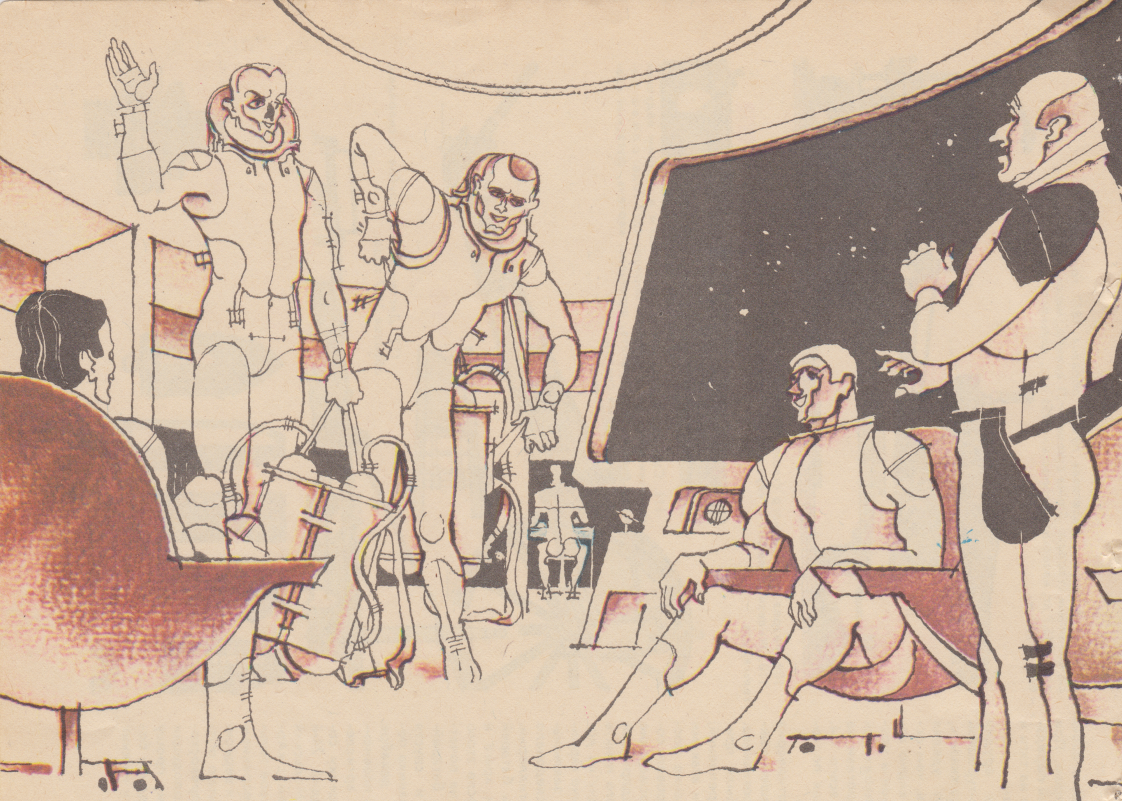
\includegraphics[width=\textwidth]{right_to_mistake}
\caption{Рис. Евгения КАТЫШЕВА}
\end{figure}

Озаренный ясным лунным светом, Коршунов возносился все выше. И вдруг мне показалось, что он ближе к стене, чем полминуты назад!

Да! Неведомая сила искривила его траекторию и тащила теперь к станции. До лестницы оставалось четыре метра, три, два... Я услышал его удовлетворенное восклицание. Коршунов протянул руку и...

Он был уже там, наверху, а я все еще здесь, нас разделяла дистанция в 600 метров, и каждый из них состоял, наверное, из пяти ступенек, итого три тысячи!..

Я вспомнил, как мы выходили к станции, вспомнил его улыбку. «В космосе нет прямых путей к цели. Ты не учитываешь центробежных сил — раз; кориолисовых сил — два; приливных сил — три... Они подкрутят «Кон-Тики» прямо в ворота...»

Тогда роль футбольного мяча исполняло наше суденышко; теперь Коршунов сам сыграл эту роль. Наверное, он ждал, что и я последую его примеру...

Я снова посмотрел вверх. Он уже скрылся из виду, я был один во всей безграничной Вселенной. Расстояние, отделявшее меня от вершины станции, казалось бесконечным. Как он прыгал? Толкнулся изо всех сил, отклонение от вертикали было ничтожным, градусов пять... Или шесть? Он уносился ввысь, а слабая кориолисова сила медленно искривляла его траекторию, влекла его назад, к станции... И так будет с любым предметом, если сообщить ему ту же начальную скорость...

Я пригнулся, шагнул под ажурное заграждение, вцепился в ступеньки и пополз вверх. Что-то сильно дернуло меня за скафандр. Страховочный трос. Я отстегнул карабин от пояса и продолжил движение.

Что чувствует муха, лишенная крыльев? Теперь я знаю это на опыте... Ступеньки кончились спустя полчаса, передо мной был край верхней площадки. В глаза брызнуло Солнце. Чья-то сильная рука ухватила меня за плечо и поставила на ноги — магнитные подошвы тут же прилипли к настилу.

— Вот и бессменный штурман «Кон-Тики» Александр Перепелкин,— услышал я знакомый, слегка ироничный голос.

Я открыл глаза. Коршунов стоял рядом, это он помог мне взобраться сюда. Площадка была так же обширна, как и на нижнем торце, но отнюдь не выглядела пустынной. В центре ее возвышалась приземистая надстройка воздушного шлюза, над входом красовался плакат: «Привет мужественным космопроходцам!» Неподалеку примостился тяжелый ракетный диск с крупными буквами на борту ТВ. У телекамер суетились люди в скафандрах. Все это что-то напоминало. Камеры были устремлены на нас. И опять, подозреваю, физиономия у меня получилась довольно глупая...

— Ну повторите, ну что вам стоит,— попросил кто-то.— Вы же профессионал...

Примечательная особенность беседы с группой незнакомцев в скафандрах — никогда не знаешь, кто из них конкретно к тебе обращается. Не фиксируется направление голоса. Пока я соображал, ответил Коршунов. Конечно, это было продолжение разговора. Начала его я не слышал — металл экранировал радиоволны, не пропускал их на мою лестницу.

— Нет,— твердо сказал Коршунов.— Мы профессионалы, но не каскадеры. Если мы иногда, как вы выражаетесь, идем на риск — а в действительности это точный расчет,—то лишь по необходимости. Сейчас я ее не вижу.

— Каскадеры! — возмутился еще один голос. Коршунов повернулся к говорившему (все они в скафандрах выглядели на одно лицо, только этот был без телеаппаратуры).— А мы, знаете, кто мы такие?

— Догадываюсь.

— Телевидение! — гордо произнес говоривший.— Причем документальное! Я режиссер...— он назвал фамилию, я ее не запомнил.— Телезрители ждут от нас правды, и мы им ее даем! У меня ответственное задание — сделать фильм о вашем полете!

— А кто вам мешает?

— Нам мешаете вы! — взорвался режиссер.— Откуда мне было знать, что вы пришвартуетесь к причалу для беспилотных зондов? Откуда мне было знать, что вы решитесь на этот сумасшедший прыжок? Откуда мне было знать, что вы откажетесь от дублей?

— Однако вы предусмотрительны,— мягко проговорил Коршунов.

— Да вы...— задохнулся режиссер.— Да мы...

— Отвяжись от него, Женя,— сказал один из людей с камерами.— Причаливание я беру на себя. Сниму старт, потом пустим обратным кадром...

— А прыжок? Я тебе должен прыгать?

— Придумаем что-нибудь,—не сдавался оператор.— Муляж бросим на леске. Леска у меня крепкая, крокодила выдержит...

В продолжение этого разговора все мы медленно продвигались к дверям шлюза. Коршунов остановился, посмотрел в небо. Солнце опускалось к дальнему краю площадки, следом Земля. Потом он шагнул внутрь, я за ним. Последними вошло телевидение. Створки за нами сдвинулись, тамбур стал наполняться воздухом. Потом гостеприимно открылся внутренний люк...

Мы провели на станции почти сутки, оставившие впечатление суматохи и хаоса. Рядом с нами все время были какие-то люди — мужчины и женщины. «Юрий Гагарин» — целый орбитальный городок, население здесь не меньше, чем в Центре Королева. Одни лица сменялись другими, все что-то спрашивали, давали советы, предостерегали. Мы обедали, мы ужинали... Равнодушных не было, все знали о рейсе «Кон-Тики». Иногда попадался режиссер Женя со своей командой либо один — без скафандра, в кожаном пиджаке и свитере, он смотрелся солиднее, действительно тянул на заслуженного. Вечерняя программа отвела нам минут пятнадцать. Снято было лихо — старт сверху и снизу, погоня за станцией, «Кон-Тики» на фоне скал... Выглядел наш кораблик весьма романтич но. Наконец заключительная сцена на верхнем причале «Гагарина»: Коршунов вытаскивает меня на площадку. Лицо у меня, кстати, получилось именно такое, как и предполагал.

Перед сном был мне вызов по видеофону. Звонил, естественно, Эдик Рыжковский все с теми же текстами. Я посоветовал ему на будущее шутить более осторожно; боюсь, это прозвучало грубо. Но я смертельно устал, и было невыносимо слушать его причитания.

После завтрака нас принял, как здесь его называют, мэр — главный администратор станции Коломин. Был еще ряд специалистов, в том числе зарубежных (станция международная), в основном по навигации и астродинамике. Обсуждали различные варианты нашего дальнейшего маршрута. Группа из Франции, как выяснилось, всю ночь гоняла свои компьютеры, теперь их руководитель докладывал результаты. Дисплей у Коломина в полстены, вверху Луна, внизу Земля, между ними по всем мыслимым траекториям болтается наш «Кон-Тики». Оказывается, если не навесить дополнительных баков, то на торможение у Земли топлива просто не хватит. Остается единственный вариант, очень красивый, он рассчитан во всех подробностях. Нам придется после отделения от станции лишь включить двигатель на определенное время, потом «Кон-Тики» сам пройдет по всей траектории, пронзит верхние слои земной атмосферы и по тормозному эллипсу выйдет на рандеву с околоземной станцией «Коперник». Топлива в этом варианте не только вполне хватит, но еще и останется, причем довольно много. Очень экономичная схема. Никто, правда, на таких судах, как «Кон-Тики», в атмосфере не тормозился, но они просчитали всю аэродинамику, все получается превосходно. Минимальная высота у нас будет семьдесят километров, перегрузки сносные, тормозить будем куполом, днищем опасно — там баки с топливом. На дисплее маневр выглядел завлекательно — кругом огонь, искры во все стороны... Телевидение — а оно, конечно, присутствовало — засняло картину в деталях и сделало необходимые дубли. Все согласились, что нужно лететь именно так, потому что никак иначе не удастся. Потом слово взял Михаил Коршунов. Он от имени экипажа поблагодарив всех присутствующих за участие, особенно французскую группу, которая за такой короткий срок подготовила столь точно рассчитанный, очень экономичный и во многих отношениях безупречный проект. Особенно Коршунову понравились расчеты торможения в атмосфере; они по-настоящему впечатляют. Его, Коршунова, в этой схеме перелета устраивает абсолютно все, за исключением одной-единственной малости: данная схема отводит ему и штурману Перепелкину, бесспорно, героическую, но не слишком вдохновляющую роль подопытных обезьян. Ибо все, что данная схема требует от командира «Кон-Тики»,— это выставить курс по какой-то там звезде и запустить движок, а от штурмана — пристально смотреть на хронометр и издать громкое восклицание в тот момент, когда движок нужно выключить. Эта работа не для человека и даже не для робота — даже роботу не понравится ощущать себя подопытной обезьяной. А он, Коршунов, и его штурман Перепелкин не роботы: оба они люди, которые умеют летать. И, надо сказать, любят это дело. Поэтому экипаж «Кон-Тики», несмотря на всю свою признательность по отношению к авторам доложенного проекта, вынужден его отклонить. «Кон-Тики» пойдет своим путем, и это вопрос решенный.

— Есть еще одно обстоятельство,— продолжал Коршунов.— Возможно, оно покажется несущественным, но для меня оно таковым не является. Я не компьютер, а человек, и мне свойственно делать ошибки. Поэтому я не могу выбрать путь, на котором обязан действовать безошибочно. Если, конечно, у меня есть выбор. Нет, я предпочту вариант, который оставляет мне право на ошибку и одновременно возможность ее исправить. Даже вернуться с полпути, если будет необходимо. Мы на периферии привыкли действовать именно так, потому что нам не на кого рассчитывать, кроме как на самих себя. Пусть этот путь не столь экономичен и эффективен, зато он гибче, он дает время собраться с мыслями, он, надежнее.

Коршунов ткнул указкой в Луну на дисплее.

— Четверть дороги пройдена,— сказал он.— Теперь у нас появились три вещи: пустые баки, возможность их наполнить и время для размышлений. И мы пойдем не прямо на Землю, как здесь предлагалось, мы пойдем во внутреннюю точку либрации.— Он показал куда-то между Луной и Землей.— Хватит полторы тонны, в крайнем случае две. Там находится автоматический танкер «Лагранж», и это все, что нам требуется. Когда мы придем туда, у нас опять будут те же три вещи: пустые баки, возможность их заправить и время для размышлений. От «Лагранжа» мы могли бы идти в атмосферу, как здесь предлагалось, и это гораздо проще, чем идти в атмосферу отсюда, но мне не очень-то нравятся игры в духе Вильгельма Телля, особенно когда приходится целить даже не в яблоко, а в его кожуру. Но после заправки нам хватит топлива на переход к Земле и обычное торможение, обычный переход на орбиту без всяких тормозных эллипсов. И вот мы уже на орбите, на своей, а «Коперник» на своей, и у нас вновь есть время для размышлений, и мы цепляемся за станцию и выходим к ней примерно так же, как вышли к «Гагарину», и у нас снова появляются три вещи: пустые баки, то, чем их можно заполнить, и время для размышлений. Вот как мы пойдем, и почти всюду на этом пути у нас будет возможность исправить ошибку, если мы ее сделаем.

И он сел, и никто уже не отговаривал нас, и только режиссер Женя шептался со своей командой на ту тему, что в точку либрации никого посылать не следует, там нет ничего интересного, это можно снять на макете, а на «Копернике» у них оператор есть, так что им остается заснять наш старт с нескольких точек, чтобы потом обратным кадром показать заодно и причаливание.

Словом, план был выслушан и одобрен, и никому из присутствовавших нельзя поставить в вину, что на деле события развернулись куда драматичнее...

Записал Михаил ПУХОВ

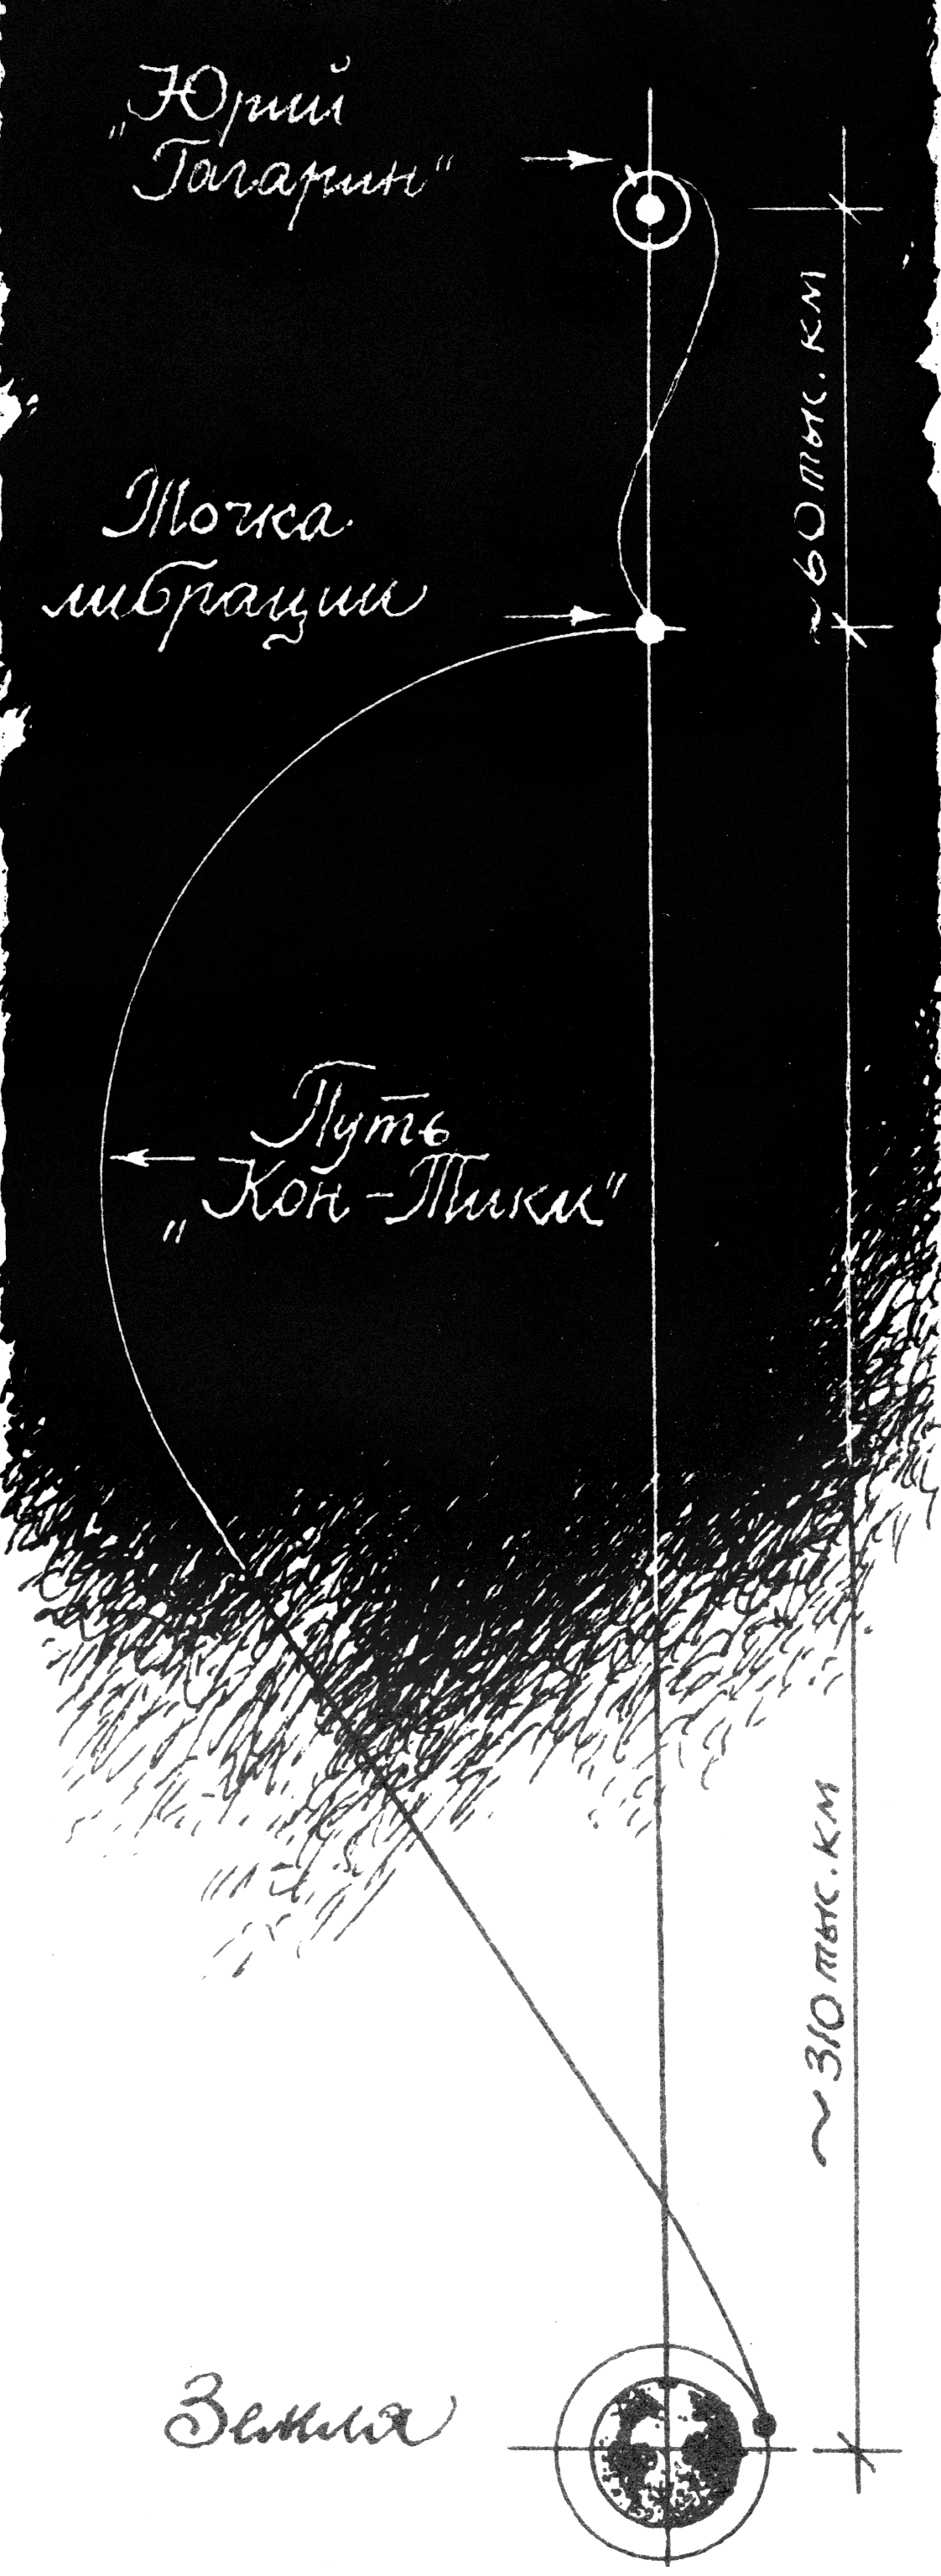
\includegraphics[width=0.25\textwidth]{ug2}

\subsubsection{Мягкой посадки}

Как видим, в историю рейса «Кон-Тики» властно вторгаются разнообразные видеосредства: звонит по видеофону селенолог Эдик Рыжковский, устраивает засады документальное телевидение во главе с режиссером Женей, дисплей в кабинете мэра орбитальной станции Коломина рисует различные варианты маршрута «Кон-Тики»...

Что может противопоставить скромный ПМК «Электроника БЗ-34» («МК-54») всему этому великолепию?

ПРЕДЛАГАЮТ ЧИТАТЕЛИ

Получаемые из сообщения ЕГГОГ буквенные шифры и видеосообщения (см. предыдущие выпуски) привлекли внимание многих читателей «ТМ». «Меня очень заинтересовали эти не отраженные в инструкции приемы,— пишет, например, С. Крутских из Горького,— поэтому очень прошу рассказать о них подробнее на страницах журнала... Этим вы окажете большую помощь по лучшему использованию этих прекрасных ПМК мне и моим друзьям, также увлекающимся программированием». Делятся читатели и своими собственными исследованиями в этой области. «Получать можно и другие символы,— пишет десятиклассник из Белгорода Д. Кайков.— Например, Е (извлечь квадратный корень из минус единицы, нажать ВП, стрелку вверх и изменить знак) или С (получить символ Г, записать его в один из регистров с номерами 0-3, отдать команду косвенного вызова из этого регистра КИП, затем команду обычного вызова из этого регистра ИП и нажать стрелку вверх). Полученные символы также можно комбинировать с различными цифрами. Например, с цифрами порядка: от —99 до — 1. и от 08 до 99».

Самостоятельно пришел к аналогичным результатам А. Соколовский из Ростова-на-Дону. Он пишет: «Эти символы можно «умножать» на 10 в любой дозволенной степени, используя ВП. Во-вторых, возможно получение Е с любым набором цифр после этой буквы, для этого достаточно набрать вместо 100, 101, 102 (имеется в виду алгоритм получения Е01, Е00, Е02 в статье И. Данилова из «ТМ» № 6.— Ред.) любое другое число, причем старшая цифра пропадает, а все остальные присоединятся к Е. В-третьих, из алгоритма получения Г извлекается алгоритм получения точки, для этого из него убирается одно ВП. В-четвертых, из (Е...) можно получить символы (Г...), (С...), (L...), (—...), где точками я обозначаю любые цифры. Для этого в режиме АВТ получают в одном из регистров 0—3 символ Е (10 ВП 99 ВП 1 /—/ П0), потом, перейдя в режим ПРГ, нужно набрать одну из команд косвенной адресации по этому регистру (я пользовался КИП) и, перейдя в режим АВТ, сделать В/О ПП необходимое число раз... Можно комбинировать эти действия с увеличением или уменьшением числа в регистре в 10, 100 и т. д. раз, то есть переносить десятичную точку».

Легко подсчитать, что предлагаемые читателями методы предоставляют в распоряжение владельца ПМК несколько миллиардов (!) различных шифрованных сообщений. Более того, если в одном из регистров записана, например, буква Е, то с помощью команд /—/ и ВП можно вывести на индикатор ровно 398 различных шифров, что, конечно, с лихвой перекрывает потребности лю
бой счетной программы.

Что можно добавить к сообщениям читателей? Во-первых, самый, по-видимому, простой способ формирования Е с любым цифровым «хвостом» — это набрать на клавиатуре соответствующее число, отдать любую «неправильную» команду, начинающуюся с К (например, К Сх), а после появления на индикаторе сообщения ЕГГОГ нажать ВП и стрелку вверх. (Этот способ неоднократно использовался в предыдущих выпусках «Клуба электронных игр».) Во-вторых, для получения С, L и т. д. довольно удобен оператор цикла — соответствующий пример будет приведен ниже. В-третьих, любое одно- и двухбуквенное сообщение (типа Е, Г, С, Е0, Г2 и т. д.) с помощью команды F 10х легко переводится в «экспоненциальную» форму — слева на индикаторе горит единица, справа — исходное сообщение (оно может быть как положительным, так и отрицательным). В-четвертых, «экспоненциальные» шифры с помощью команд ВП /—/ 1 и ВП /—/ 10 (после них следует нажать стрелку вверх) легко преобразуются в новые шифры такого же вида. В-пя- тых, каждый «экспоненциальный» шифр переводится командой К Сх (с последующим нажатием ВП и стрелки вверх) в аналогичный шифр, в котором единица заменена буквой Е (эти шифры, в свою очередь, с помощью уже рассмотренной команды ВП /—/ 1 или 10 столь же легко преобразуются в новые). Все эти способы неоднократно использовались в наших выпусках, в том числе для получения видеосообщений типа: «Космический корабль над обратной стороной Луны».

Приведенных сведений достаточно, чтобы перейти к демонстрационному мультфильму «Кон-Тики», смонтированному пятиклассником Сергеем Пуховым из тех самых буквенных шифров и видеосообщений, о которых шла речь выше. Значит, не только телевидение XXI века заинтересовал этот рекордный рейс!.. Подготовка к показу данного фильма по времени многократно превышает его продолжительность, что лишний раз подтверждает простую истину: то, что мы видим на экране, являет собой всего лишь «верхушку айсберга», основная масса которого скрывается от нашего взора в темных океанских глубинах...

Первое, что нужно сделать,— это ввести в ПМК вспомогательную программу преобразования видеосообщений с помощью оператора цикла, о котором уже говорилось:

00.П1 01.ИП1 02.С/П 03.FL1 04.01

Как видим, в ней нет ничего, кроме записи в регистр 1, вызова из этого регистра, останова и цикла по этим командам. Теперь можно приступать к формированию кадров будущего фильма (в скобках для контроля приводятся показания индикатора). Итак, F АВТ В/О Сх (0) С/П (0) С/П (—99999999) КСх (ЕГГОГ) ВП /—/ 1 В/О С/П (—Е999999.9) С/П (—9Е999998) КСх (ЕГГОГ) ВП В/О С/П (—ЕЕ999998) /—/ ВП /—/ 5 В/О С/П (ЕЕ9.99998) С/П (ЕЕ8) С/П (ЕЕ7) С/П (ЕЕ6) С/П (ЕЕ5) С/П (ЕЕ4) С/П (ЕЕЗ) С/П (ЕЕ2) С/П (ЕЕ1) С/П (ЕЕО) ВП /—/ 1 ПД (ЕЕ) В/О С/П (ЕЕ) С/П (ЕГ) С/П (ЕС) С/П (EL) С/П (Е—) ВП /—/ 1 П3 (Е.—) ВП 1 F 10$^{x}$ (слева на индикаторе единица, справа ноль) КСх (ЕГГОГ) ВП П9 (слева Е, справа 0) ИПД /—/ F 10$^{x}$ (слева единица, справа — ЕЕ) КСх (ЕГГОГ) ВП /—/ 11 П4 (слева Е, справа минус) ВП /—/ 10 П8 (сообщение «Корабль над видимой стороной Луны», оно нам знакомо по «ТМ» № 9) ИП4 ВП /—/ 1 П5 (похожее сообщение, корабль сместился к Земле) ИПД F 10$^{x}$ КСх (ЕГГОГ) ВП /—/ 44 ПД (слева Е, справа два минуса) ВП /—/ 9 ВП /—/ 1 П6 (видоизмененное сообщение «Корабль над видимой стороной») ИПД ВП /—/ 90 ВП /—/ 10 П7 (сообщение «Корабль над обратной стороной Луны») 1 КСх (ЕГГОГ) ВП П1 /—/ П2 (—Е) В/О. Подготовительная работа закончена, все кадры электронного фильма «Кон-Тики» записаны в адресуемые регистры 1—9.

Теперь нужно перейти в режим программирования и ввести в ПМК демонстрационную программу «Мультфильм» — она будет извлекать кадры в нужной последовательности. Программа очень короткая, хотя использует и команду косвенного вызова, и оператор цикла:

00.Сх 01.9 02.П0 03.КИП$\uparrow$ 04.С/П 05. FL0 06.03 07. В/0

Чтобы полюбоваться теперь видеофильмом о путешествии «Кон-Тики», надо вернуться в режим вычислений (F АВТ В/О) и нажать С/П. Фильм «Кон-Тики» состоит в общей сложности из 9 кадров, с некоторыми мы уже сталкивались в предыдущих программах, с другими еще встретимся. Как и в «ТМ» № 9, Е означает Землю, 0 — Луну, знак «минус» — лунолет «Кон-Тики». Переход от кадра к кадру осуществляется командой С/П

\begin{enumerate}
\item Система Земля — Луна перед стартом «Кон-Тики».
\item Старт.
\item Над обратной стороной Луны.
\item «Кон-Тики» завершает виток.
\item Старт с окололунной орбиты.
\item «Кон-Тики» на полпути к Земле. Луна справа за кадром.
\item «Кон-Тики» в окрестностях Земли.
\item На околоземной орбите.
\item Финиш.
\end{enumerate}

Если продолжать нажимать С/П, фильм будет повторяться неограниченное число раз. Надеемся, что приведенная программа и подготовительные операции к ней помогут вам в овладении «скрытыми» возможностями ПМК.

Наше очередное задание несложное, зато полезное. Оно связано с получением различных видеосообщений, пригодных для использования в электронных играх.

\begin{enumerate}
\item Используя приведенную выше процедуру, сформировать шифры ЕЕ и —EL. Применив к ним команду F 10$^{x}$, получить соответствующие «экспоненциальные» сообщения (единица слева, справа показатель). Используя команды ВП /—/ 1 и ВП /—/ 10, получить из базовых все остальные допустимые показательные сообщения. Составить сводную таблицу таких сообщений (нам ее высылать не обязательно, у нас она уже есть, в ответе достаточно указать количество получившихся у вас сообщений).
\item Выбрать из получившейся таблицы шифры, которые, на ваш взгляд, полезны для использования в электронных играх, и дать их интерпретацию.
\end{enumerate}

Клуб электронных игр поздравляет всех участников перелета Луна — Земля с наступающим Новым годом. Желаем хорошо отдохнуть на борту гостеприимной станции «ЮГ», но формы не терять: впереди нас ожидают суровые  испытания. До Земли еще очень и очень далеко (см. схему).

С Новым годом!

Опечатки. В программе «Лунолет-2» (№8) по адресу 23 должно стоять Fx=0. В программе «Лунолет-1 М» (№ 10) по адресу 22 должна стоять стрелка вверх.

\subsection{ТЬМА}
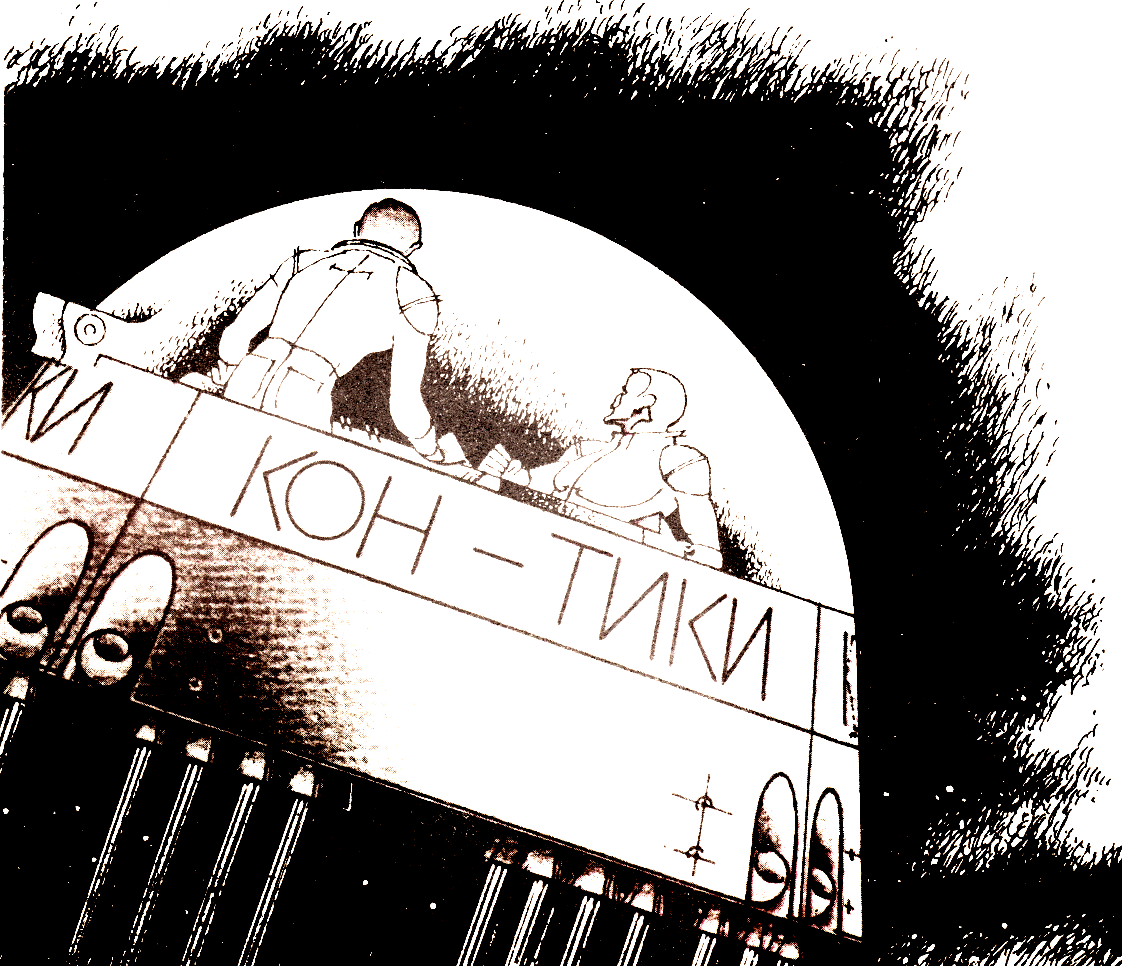
\includegraphics[width=0.5\textwidth]{darkness}
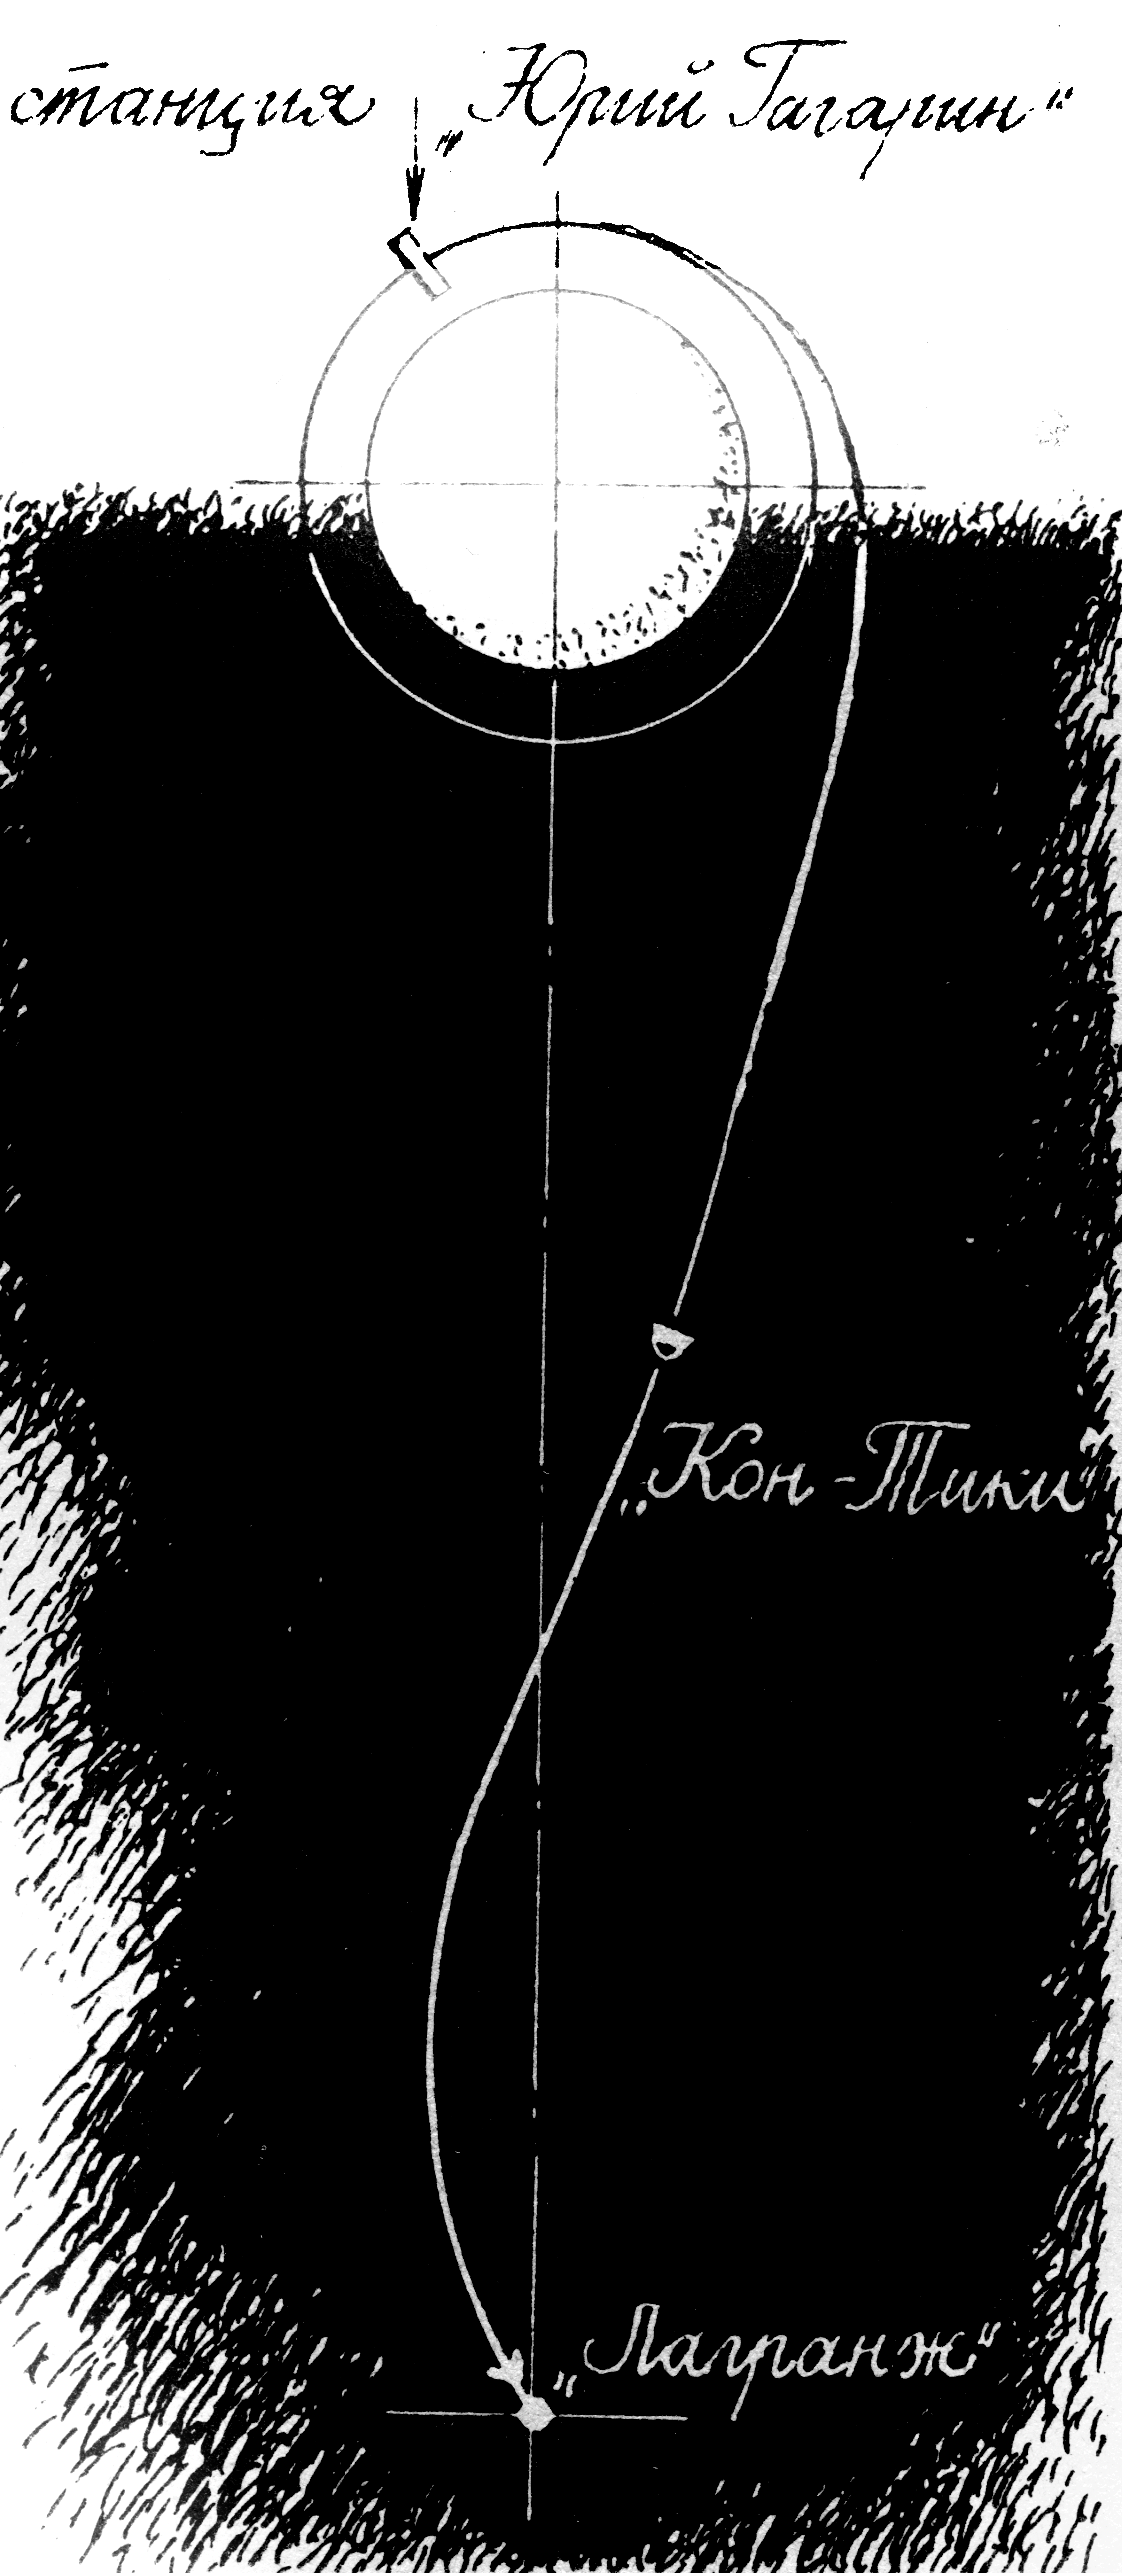
\includegraphics[width=0.5\textwidth]{darkness2}

Мы продолжаем публикацию документально-фантастического отчета «Путь к Земле» (см. № 8-12 за 1985 год). Вкратце напоминаем содержание предыдущих глав. Бывший космонавт Михаил Коршунов (Лунный Коршун) возвращается домой из системы Юпитера. Решив тряхнуть стариной, последний отрезок пути (Луна — Земля) он собирается проделать самостоятельно, на первом попавшемся транспортном средстве. Селенолог Эдуард Рыжковский в порядке розыгрыша предлагает ему свой крохотный лунолет, не приспособленный для космических полетов. Коршунов принимает вызов. По иронии судьбы штурманом «Кон-Тики» (так нарекает Коршунов свой лунолет) становится Александр Перепелкин, не имеющий никакого отношения к космонавтике. От его лица и ведется повествование. Мужественно справившись с непреодолимыми, казалось бы, трудностями, после многочисленных приключений экипаж «Кон-Тики» прибывает на окололунную орбитальную станцию «Юрий Гагарин». Цель нового рискованного броска — внутренняя точка либрации, где находится автоматический танкер «Лагранж». Здесь намечено пополнить запасы топлива и идти затем к околоземной станции «Коперник».

Каждый выпуск сопровождается игровыми программами, с помощью которых читатели, умеющие обращаться с программируемыми микрокалькуляторами «Электроника БЗ-34» («МК-54»), могут самостоятельно повторить важнейшие этапы этого небывалого путешествия, а также при желании совершать другие сложные космические операции.

Стартовая площадка была ярко озарена прожекторами. Несомненно, свет некоторых из них, невидимый в вакууме, рыскал сейчас в темноте в поисках «Кон-Тики», но усилия были тщетными — Коршунов ловким маневром ушел из следящего луча, а вновь нащупать столь утлое суденышко в глубине космоса смогла бы разве что автоматическая противометеоритная система. Однако данными прожекторами руководили вовсе не роботы.

Мы снялись с верхней палубы «Гагарина» (а сюда перегнал «Кон-Тики» кто-то из местной стартовой команды ночью, пока мы спали) над центром обратной стороны Луны, несмотря на настойчивые уговоры ТВ подождать до стороны освещенной, на которой условия съемки гораздо предпочтительней. Мы были неумолимы. Пришлось им прибегнуть к искусственному освещению, а теперь, после маневра Коршунова, оно стало бессильным и бесполезным. До станции все еще было рукой подать — она выглядела черной прямоугольной тенью на фоне звездного неба, окаймленной ходовыми огнями, верхняя же площадка казалась самостоятельным летательным аппаратом, подобным Лапуте, на которой некогда побывал Гулливер.

Мы уходили от станции со скоростью пешехода — разгон, по мнению Коршунова, следовало начать минут через 10-15 после старта. Так мы гораздо точнее выйдем к «Лагранжу» и сбережем много топлива. Хотя, казалось бы, чего там особенно экономить — все равно заправляться...

— Полный порядок,— сказал Коршунов. В кабине было темно, только  неярко мерцали индикаторы на пульте управления.— Они нас уже не найдут. Рассказывай, что было дальше.

Утро для меня началось с хлопот по снабжению и заправке «Кон-Тики». Прикинув, что до «Лагранжа» нам с лихвой хватит тонны топлива, я поставил в заявке на всякий случаи «1500 кг» и дал подписать Коршунову. Он изучал бланк несколько секунд, потом исправил 1 на 3 и расписался внизу. «Лихость твоя мне нравится,— ответил он на мой недоуменный вопрос.— Ты все рассчитал правильно. Но мы идем в космос, не на орбиту, впереди сутки полета. В таких случаях лучше иметь запас на обратный путь, раз уж есть возможность. Мало ли что может случиться».

По второй части заявки — воздух, вода и прочее на 10 суток — замечаний у него не возникло. «Именно десять. Больше десяти дней не продержимся, обязательно куда-нибудь свалимся». Я взял подписанный документ и отправился в диспетчерскую. Там-то и начались непредвиденные осложнения, о подробностях которых Коршунов желал сейчас услышать. Я сунул бланк в приемную щель машины, и та незамедлительно выплюнула его обратно! На дисплее зажглась надпись: «Не указана цель полета».

— А ты что? — спросил Коршунов.

В общих чертах он уже знал о происшествии, был осведомлен и о результатах, сейчас его интересовали детали.

— Я написал на бланке «Земля» и сунул бумагу обратно в машину.

— Молодец! — похвалил Коршунов.— А она?

— Тут же выбросила назад. На дисплее загорелось: «Заправка не разрешается. Судно не приспособлено для полета к планетам, имеющим атмосферу. В заявку следует включить требование об установке на судно стабилиза- торов и тормозных щитков».

— А ты? — спросил Коршунов. Зная его «любовь» к компьютерам, нетрудно понять, что ситуация его развлекала.

— Я, естественно, зачеркнул слово «Земля», вписал «Луна» — и туда же.

— Находчиво! — определил Коршунов и посмотрел на часы.— Кажется, нам пора. Держись, штурман!

Двигатель загремел. Разгонялся Коршунов, как всегда, на предельном режиме. Ускорение продолжалось с полминуты. Когда двигатель умолк, станция потерялась позади, а цифры на указателе топлива уменьшились ровно на тонну.

— Скорость? — осведомился он.

— Параболическая! — сказал	я.— Даже немного больше...

— Нехорошо,— поморщился он в тусклом свете индикаторов.— Терпеть не могу парабол. Чуть меньше скорость — и сваливаешься на эллипс. Чуть выше — ты уже на гиперболе. А между ними — дистанция огромного размера. Давай-ка для надежности бросим еще литров двести. Не оптимально, конечно, зато выиграем много часов. Гипербола — единственная порядочная кривая...

Двигатель загрохотал снова, на сей раз всего на несколько секунд. Потом замолчал — очень и очень надолго.

— А что дальше? — спросил Коршунов.— Ты написал «Луна»...

— Она опять вернула заявку. Теперь на дисплее значилось: «Заправка не разрешается. Судно не приспособлено для полета к планетам, не имеющим атмосферы. В заявку следует включить требование об установке на судно посадочных амортизаторов».

— Я волком бы выгрыз бюрократизм! — с чувством процитировал Коршунов.— Тебе следовало назвать второй причал «Гагарина».

— Я думал об этом. Проклятая машина не выделила бы нам трех с половиной тонн топлива и ресурса на десять дней для перелета с причала на причал. Я исправил «Луна» на «Земля» и вписал требование насчет тормозных щитков. В результате «Кон-Тики» утяжелился на полсотни килограммов. Но если бы я оставил «Луна», навеска была бы вдвое тяжелее. Правда, еще не поздно от них отделаться.

— Я смотрел,— сказал Коршунов.— Приварено насмерть. Но не огорчайся, штурман. Может, еще пригодятся. Кто знает...

Я не ответил. Впереди вспыхнула огненная линия горизонта. Затем появилось Солнце. Его лучи озарили пейзаж под нами: бесчисленные кратеры, очень рельефные при боковом освещении. Они не только уносились назад — к этому мы успели привыкнуть,— но и уменьшались буквально с каждой минутой. «Кон-Тики» набирал высоту, и это было заметно на глаз. Луна стала уже шаром — громадным, но отчетливо выпуклым. Высота росла: 200 км, 300, 400...

— Вот и она! — Коршунов показал вперед. Над горизонтом поднималась облачная дуга Земли — словно птица с отогнутыми назад крыльями.— Несколько дней, и мы будем там. Не верится?..

С момента отделения от станции прошло каких-то полчаса. Высота увеличивалась: 600 км, 700, 800... Луна съеживалась, по площади она занимала, наверное, всего процентов десять небесной сферы.

— Запомни этот момент, штурман! — Цифры на альтиметре быстро сменялись: 1650 км, 1700, 1750...— Шельф кончился, впереди открытое море!

Да, мы удалились от Луны на величину ее радиуса, траектория задиралась все круче. К исходу первого часа поднялись более чем на три тысячи километров, Земля уверенно подбиралась к зениту, вектор скорости запрокидывался. Мы шли к Земле, это было несомненно. Луна все еще доминировала в небе, но была уже не внизу, а позади нас!

— Завтра заправимся,— мечтательно проговорил Коршунов.— А через недельку, глядишь, будем сидеть где-нибудь на бережку, на камушках, и потягивать из синего моря рыбку — большую и маленькую. Настоящую рыбку, Саша...

— Что значит «настоящую»? — поинтересовался я.

— Ну, у нас, на спутниках Юпитера,— объяснил он,— ты знаешь, тоже есть океаны. Подо льдом, можно сказать, бездонные. Но они, в отличие от земных, безжизненны. Так, по крайней мере, считалось. Вот уже много лет в системе Юпитера работает несколько биологических станций. Биологи пытаются заселить местные океаны земными формами жизни. Вода — она всюду вода. Да ты слышал об этом, Саша...

— Только краем уха,— возразил я.— Знаю, что такие опыты проводились, но ничего конкретного. Слишком далеко от моей обычной работы.

— Правда? — оживился он.— Что ты, за последние годы результаты получены просто отличные. Отличные от всего, что кто-либо ожидал. Теперь в поставленную ловушку нетрудно поймать, например, семгу, угря или даже треску. Но может забрести туда и чудовище... А они страшные, Саша.

Он замолчал.

— Насчет семги или даже трески мне понятно,— сказал я.— Но откуда взялись чудовища?

— Никто не знает. То ли какие-то мутации. То ли там всегда водилась эта нечисть. То ли возникли гибриды местных и земных форм. Некоторые из этих существ ужасны на вид, но вполне безобидны и даже полезны во многих отношениях. В гастрономическом, например. Зато есть и такие, которые рвут любые сети и приводят в полную непригодность самые изощренные ловушки. Есть существа-оборотни, принимающие любые обличья. А самое страшное из них называется Тьма...

— Тьма? — Жутким, нездешним холодом веяло от этого названия.— Почему именно Тьма?

— Никто ее толком не видел, Саша,— сказал Коршунов.— Никто из ныне живущих. Человек, столкнувшийся с Тьмой, гибнет. Приборы выходят из строя, пленки стираются и засвечиваются. Никто из живых не видел ее, но все-таки она существует. Опасное это дело — охота в системе Юпитера...

Время тянулось медленно. Центр Королева вышел из-за горизонта, был где-то внизу, но мы его, конечно, не видели. Земля переместилась в зенит, «Кон-Тики» поднимался почти вертикально со скоростью порядка километра в секунду. Через четыре часа позади осталась уже четвертая часть пути, спустя еще пять — практически половина. Луна стала отдаленным небесным телом — ее угловой диаметр превышал земной всего раза в три. До точки либрации оставалось тридцать тысяч километров и пятнадцать часов пути, мы шли к цели точно, по очень вытянутой дуге, можно было и отдохнуть. Разложили кресла, Коршунов сориентировал «Кон-Тики» днищем вперед, отгородив кабину от солнечного света. Сразу стало темно. Нас окружал мрак, светлая темнота, черное небо, усыпанное бесчисленными мелкими звездами. Воображение услужливо извлекало из памяти картины прошедшего дня.

«Человек, столкнувшийся с Тьмой, гибнет»,— вот последняя фраза, которая всплыла у меня в сознании перед тем, как уснул.

Снилось тоже нечто жуткое и нездешнее: бесформенная тягучая субстанция окружала меня, душила, увлекала в черную вибрирующую пустоту... Вибрация, сначала еле заметная, вскоре стала невыносимой.

Я открыл глаза и сразу увидел звезды. Коршунов тряс меня за плечо.

— Проснись, Саша,— сказал он мягко.— Дурные новости. Метеоритная атака, «Лагранж» не отзывается на сигналы. Думаю, топлива мы теперь не получим...

\subsubsection{МЯГКОЙ ПОСАДКИ!}
Похоже, с автоматическим танкером «Лагранж» случилось непоправимое, и мечты о пополнении запасов топлива придется оставить до лучших времен. Тем не менее остановка в точке либрации необходима: во-первых, нужно выяснить, что же все-таки стряслось с танкером, во-вторых, в этой точке, где все гравитационные и инерционные силы уравновешены, можно спокойно, без спешки проанализировать ситуацию и подумать, как быть дальше. Что ж, этот солидный по протяженности отрезок пути (более 60 тыс. км в использованной приближенной модели) вполне под силу нашему стандартному «транспортному средству» — ПМК «Электроника БЗ-34» («МК-54»), оснащенному новой программой «Лунолет-4».

00.Сх 01.2	02.$\div$ 03.ИПА 04 + 05.ПА 06.ИП1
07.- 08.ИПА 09.ИП7 10.- 11.С/П 12.П9 13.П8 14.П2 15.$\div$ 16.ИП6 17.x 18.ИПД 19.ИП8 20.- 21.Fx$\geq$0 22.00 23.ПД 24.ИП5 25.+ 26.$\div$ 27.П8 28.ИПС 29.Fsin 30.ИПВ 31.ПП 32.74 33.Fsin 34.x 35.ПП 36.70 37.ИП0 38.+ 39.П0 40.ПП 41.69 42.9 43.0 44.x 45.F$\pi$ 46.$\div$ 47.ИПА 48. $\div$ 49.ИПС 50.+ 51.ПС 52.Fcos 53.ИП0 54.ПП 55.74
56.Fcos 57.x 58.- 59.ИП4 60.ИПА 61.Fx$^{2}$ 62.$\div$ 63.ПП 64.70 65./-/ 66.ИПВ 67.+
68.ПВ 69.FBx 70.+ 71.ИП2	72.x 73.В/0
74.ИП0 75.ИПА 76.$\div$ 77.ИП3 78.+ 79.ИП3 80.+ 81.x 82.\XY 83.ИПС 84.Fcos 85.x
86.ИПА 87.x 88.3	89.x 90.ИП3 91.Fx$^{2}$ 92.x
93.+ 94./-/ 95.ИП8 96.ИП9 97.В/О

Она предназначена для численного моделирования различных маневров космических аппаратов вблизи безатмосферного небесного тела (луны), вращающегося по круговой орбите вокруг другого небесного тела (планеты) и, подобно нашей Луне, постоянно обращенного к планете одной своей стороной. Программа учитывает влияние планеты на движение аппарата и позволяет выполнить принципиально новую космическую операцию — перелет во внешнюю или внутреннюю; точку либрации (они в использованной модели располагаются на линии планета — луна на равных расстояниях от центра луны), зато не приспособлена для посадки — автоматический контроль контакта с поверхностью здесь отсутствует. Исходные данные в основном те же, что и в «Лунолете-3» (см. «ТМ» № 9 за 1985 год): (масса космического корабля без топлива, кг) П5 (радиус луны, м) П7 (скорость истечения продуктов сгорания, м/с) П6 (расстояние до центра луны, м) ПА (вертикальная скорость, м/с) ПВ (угловое расстояние от центра видимой стороны луны, градусы) ПС (запас топлива, кг) ПД. Другие связаны с новым характером решаемой задачи. В регистр 4 вводится так называемая гравитационная постоянная луны, равная произведению ускорения силы тяжести на ее поверхности на квадрат радиуса. Нужно набрать на пульте ускорение силы тяжести (для нашей Луны — 1,62) и команду ИП7 Fx$^{2}$ X П4. В регистр 3 вводится угловая скорость обращения луны вокруг планеты, для этого нужно сначала рассчитать гравитационную постоянную планеты: (радиус планеты, м) Fx$^{2}$ (ускорение силы тяжести на поверхности планеты, м/с$^{2}$) X, затем набрать радиус орбиты луны в м (для нашей Луны 3844 ВП 5) и команду Fx$^{2}$ FBx X $\div$ F$\sqrt{}$ ПЗ. В регистр 1 вводится расстояние от центра луны до точки либрации: 3 F1/x $\uparrow$ ИП4 ИПЗ Fx$^{2}\div$ X Fx$^{y}$ П1. Осталась горизонтальная скорость корабля. Если он в начальном положении находится на круговой окололунной орбите, то она рассчитывается как обычно: ИП4 ИПА $\div$ F$\sqrt{}$, только теперь нужно еще вычесть из полученной величины скорость, связанную с вращением луны вокруг своей оси: ИПЗ ИПА X— П0. (Предполагается, что направления движения корабля и вращения луны совпадают; в противоположном случае в последней формуле вместо — надо поставить +.) Наконец, как обычно, В/О С/П.

При останове на индикаторе появляется текущая высота полета, в регистре У находится расстояние по вертикали до точки либрации. Остальные переменные — расстояние до центра луны, вертикальная и горизонтальная скорости, угловое расстояние до центра видимой стороны луны, текущий запас топлива — находятся в регистрах А, В, О, С, Д и вызываются командами ИПА, ИПВ, ИП0, ИПС, ИПД. Маневр задается традиционно: (угол отклонения вектора тяги от вертикали, градусы) ПП (расход топлива, кг) ПП (время., с) С/П. Переключатель Р—Г должен быть установлен в положение Г, команда с перерасходом топлива блокируется.

При дальних вылазках в космическое пространство на «Лунолете-4» рекомендуется придерживаться следующих правил: во-первых, выполнять перелет на гиперболических скоростях (параболическая скорость в $\sqrt{2}$ больше круговой, а гиперболические соответственно еще выше); во-вторых, в свободном полете на высотах, не превышающих диаметра луны (для нашей Луны около 3500 км), задавать время маневра не более 300 с, затем переходить на 1000-секундные интервалы, при удалении на 15 тыс. км
можно уже задавать часовые интервалы (порядка 3000 с), а начиная с 30 тыс. км — трехчасовые (10 000 с). При прикидочном выходе в точку либрации полезно следовать указаниям, содержащимся в 6-й части отчета А. Перепелкина.

\subsubsection{ОХОТА НА «ИНОПЛАНЕТНЫХ ЧУДОВИЩ»}

Скажем честно: в недрах любой вычислительной системы, в частности и нашей «Электроники», обитают не менее диковинные создания, чем те, которые населяют глубины европеанских океанов и о которых упоминает командир «Кон-Тики». На индикатор ПМК, как известно, выводятся числа, не превышающие по величине 9,9999999 ВП 99 (9,9999999— мантисса, 99 — порядок числа). Они для нас столь же привычны, как и обычные рыбы земных водоемов. Однако «Электроника БЗ-34» способна формировать числа гораздо большие (с порядком до 1000!), причем при соответствующем навыке каждое из них можно «изловить» (записать в регистр), проанализировать, а затем как-то использовать. Конкретный вид и свойства этих «арифметических чудищ» зависят от глубин, где они водятся (точнее, от величины порядка). «Охота» на них — занятие увлекательное и в ряде, случаев небезопасное.

Вот краткая классификация «глубоководной фауны» ПМК. Глубины (порядки) до 100 заселены обычными числами. Следующий «этаж» (от 100 до 200) принадлежит ЕГГОГам; еще глубже (от 200 до 300) обитают ЗГГОГи — создания, вопреки своему зловещему виду, в высшей степени полезные, их легко приручить.

Далее (от 300 до 400) располагается вотчина диких и неукротимых чудовищ, норовящих при малейшей оплошности со стороны охотника привести программу в негодность и заставить его выключить ПМК. Следующий этаж (от 400 до 500) заселен ОС-оборотнями — существами очень полезными, но, в свою очередь, подразделяющимися на многочисленные семейства. Еще ниже (от 500 до 600) располагаются владения Тьмы, при любом контакте с этой таинственной и грозной субстанцией индикатор гаснет, и приходится отключать ПМК. (Отметим, что с Тьмой можно случайно столкнуться и на других этажах.) Глубже, за пределы Тьмы, можно проникнуть лишь с помощью специального «водолазного оборудования» (соответствующих программ): глубины от 600 до 700 заселены медлительными С—ЕГГОГ-оборотнями, еще ниже (от 700 до 800) обитают неповоротливые монстры, чьи повадки тем не менее заставляют вспомнить безудержных чудовищ 4-го этажа и охота на которых - протекает аналогично. На предпоследнем этаже (от 800 до 900) безраздельно властвует Ноль (самый обычный, насколько удалось выяснить), дальше (от 900 до 1000) начинается зона обычных чисел с постепенно уменьшающимися отрицательными порядками, наконец, после 1000 круг замыкается — на сцену вновь выступают числа с положительными порядками, затем ЕГГОГи, и все повторяется. А теперь познакомимся ближе с населением каждого этажа.

\paragraph{1-й этаж.} Здесь, как уже отмечалось, обитают обычные числа. У них, конечно, много всяких любопытных свойств (как и у самых обыкновенных земных животных), но к предмету нашего разговора они не относятся.
\paragraph{2-й этаж.} ЕГГОГи, населяющие глубины (порядки) от 100 до 200,— самые неинтересные из обитателей нашего «электронного океана». В общем-то, это обычные числа, которые можно делить, умножать, складывать, записывать в регистры, но которые не выводятся на индикатор в силу своей чрезмерной величины. Изловить ЕГГОГа проще простого: достаточно, например, отдать команду 1 ВП 50 Fx$^{2}$ П0 Сх, и ЕГГОГ (десять в сотой степени) сидит в регистре 0! Если теперь разделить его, допустим, на 10, то на индикаторе появится совершенно обыденная единица с порядком 99.
\paragraph{3-й этаж.} Если возвести ЕГГОГа из предыдущего примера в квадрат (или иным способом получить число с показателем степени между 200 и 300), на индикаторе появится ЗГГОГ. Эти числа также можно умножать, складывать, записывать в регистры и так далее. Однако, помимо этого, ЗГГОГ обладает целым рядом присущих только ему и весьма полезных качеств.

\begin{enumerate}
\item Десятичная точка при появлении на индикаторе ЗГГОГа сохраняет свое положение, как бы «наследует» его от предыдущего числа. Запишите какого-нибудь ЗГГОГа в произвольный регистр. Наберите на индикаторе любое число (в его состав, естественно, обязательно входит десятичная точка — если число целое, она его замыкает) и вызовите ЗГГОГ на индикатор. Точка осталась на прежнем месте. Это свойство позволяет использовать 3ГГОГов в электронных играх для визуальной индикации положения объекта (как сделано, например, в игре «Посадка на планету ЗГГОГ», см. «ТМ» № 10 за 1985 год; напоминаем, что в программе опечатка — по адресу 22 должна стоять стрелка вверх).
\item Всякий ЗГГОГ выполняет операцию безусловного перехода на адрес, совпадающий с первыми двумя цифрами порядка «зашифрованного» под ним числа. Так, полученный нами ЗГГОГ равен 10 в двухсотой степени; если при его появлении на индикаторе отдать команду F ПРГ, убедимся, что справа горит 20. Это свойство также использовано в № 10 — далеко не каждый ЗГГОГ годится для той игры!
\item Всякого ЗГГОГа, появившегося на индикаторе, легко «расшифровать» с помощью следующей процедуры: нажать F АВТ, затем десятичную точку — справа на индикаторе загорится трехзначный порядок числа, которое прячется под личиной ЗГГОГа. Снова нажмите F АВТ — слева на индикаторе появится мантисса числа, справа — некий новый показатель, весьма причудливый, зависящий от способа появления данного ЗГГОГа на индикаторе и для дешифровщика бесполезный. Применение этой процедуры к нашему ЗГГОГу дает порядок 200 и мантиссу 1, как, очевидно, и должно быть.
\item Предыдущее свойство подсказывает новый эффективный прием формирования показательных сообщений (о них смотри № 12 за 1985 год). Вызвав нашего ЗГГОГа из регистра, куда он был записан, и применив к нему процедуру «расшифровки», получим показатель, с которым прежде не встречались (--L). Если теперь отдать команду ВП 99 F АВТ, появится еще одно новое показательное сообщение (справа на индикаторе горит «чистая» буква Е). Из этих двух сообщений с помощью команд ВП /—/ 1 и ВП /—/ 10 легко получить все остальные мыслимые показательные шифры.
\item ЗГГОГ, записанный в регистр 9 либо 0, может использоваться как анализатор состояния программного счетчика. Убрав ЗГГОГа с индикатора, отдайте, например, команду БП 58. Вызовите ЗГГОГа и нажмите десятичную точку. Справа на индикаторе загорится 580. Данное свойство ЗГГОГа позволяет использовать его для «дешифровки» некоторых других «чудовищ», населяющих глубинные этажи нашего «числового моря».
\end{enumerate}
\paragraph{4-й этаж.} Перейдем к «охоте» на глубинах 300—400. Выберем в качестве объекта, например, число 10 в трехсотой степени. Отдаем команды 1 ВП 50 Fx$^{2}$ Fx$^{2}$ П9 (записываем ЗГГОГа для последующего использования в качестве анализатора) FBx. Все готово: в регистре Y сидит ЗГГОГ (10 в двухсотой степени), в регистре X — ЕГГОГ (10 в сотой степени). Остается их перемножить...

Караул! На экране мелькают цифры — ПМК самопроизвольно перешел в режим счета! Чудовище вырвалось на свободу и мчится по нашей пустой программе, как по бесконечному коридору! Срочно нажимаем С/П. На индикаторе ноль. Это естественно — программа пуста, она состоит из нолей, вот ноль и считался в регистр X, оттеснив чудовище в регистр Y. Чтобы взглянуть на «добычу», нужно нажать \XY...

Нас ждет новое потрясение! Вместо ожидаемого чудища мы видим перед собой лишь следы его деятельности — испорченный фрагмент программы. ПМК самопроизвольно перешел в режим программирования! Слева на индикаторе горит .0, затем две пары 00, в правом углу — 31. Значит, программа остановилась на адресе 30. По аналогии со ЗГГОГами заключаем, что это опять-таки первые две цифры порядка изловленного числа. Точка, как и у ЗГГОГа, унаследовала свое положение от предыдущего числа (только что на индикаторе горел ноль, естественно, с точкой). Наконец, левый ноль — это вторая цифра порядка (300). Если бы порядок был, скажем, 384, то слева на индикаторе горело бы .8, справа — 39.

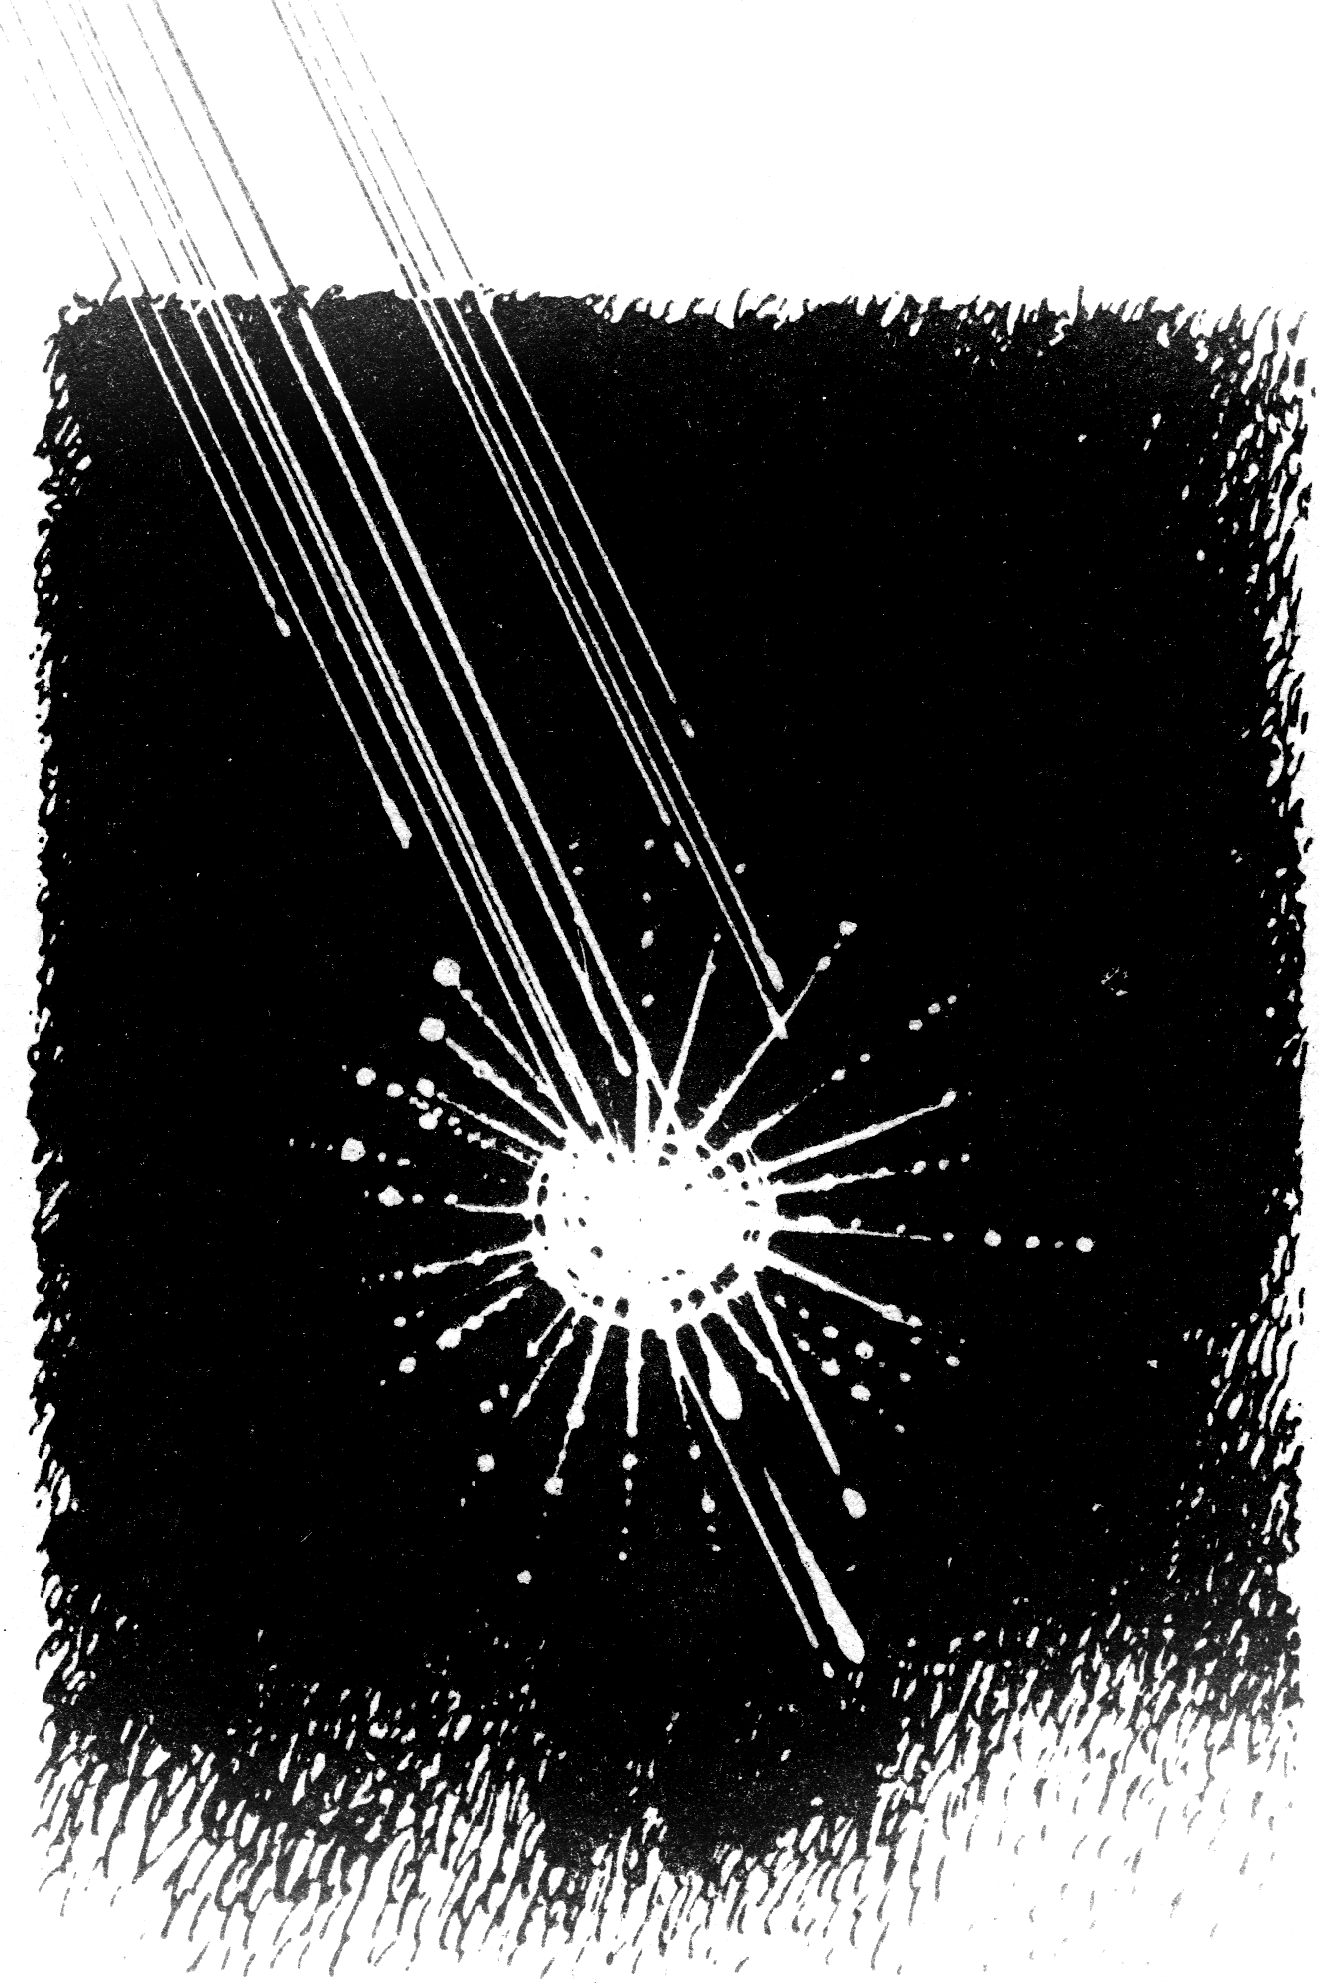
\includegraphics[width=0.5\textwidth]{darkness3}

Что делать дальше? Грубейшей ошибкой будет естественное F АВТ — ПМК зациклится на поврежденной команде и не отзовется ни на один приказ с пульта, придется его отключить. Нажимаем F ПРГ. Точка исчезает. Теперь ШГ влево. Какой командой заменить испорченную? Наша задача — поймать чудовище, поэтому впишем сюда, например, ПА. Затем Сх (чтобы очистить стек) и С/П. Вот теперь можно и F АВТ. На индикаторе тут же загорается 0 — стек чист, а чудовище сидит в регистре А! Самое время проанализировать его с помощью ЗГГОГа из регистра 9. Трижды нажимаем ШГ влево (для компенсации вписанных в программу команд), ИП9, точку (на индикаторе появляется порядок 300) и F АВТ (слева загорается мантисса — 1). Забив на всякий случай нолями вписанные в программу команды, можно начинать охоту на следующее чудовище (только не надо забывать, что первое все еще томится в регистре А, ожидая команды ИПА, чтобы оттуда вырваться!). Вся эта процедура может пригодиться и для получения совершенно конкретных практических результатов. Например, она позволяет определять факториалы чисел вплоть до 210 (воспользуйтесь любой программой, вычисляющей факториал, и проанализируйте результат с помощью ЗГГОГа из регистра 9).

Охота на 5-м уровне — в обители ОС-оборотней — не менее увлекательна, о ней мы расскажем в следующем выпуске. Уникальные свойства этих созданий подтверждаются, например, простыми алгоритмами получения знакомого нам по предыдущему номеру сообщения ЕЕ: 1 ВП 55 Fx$^{2}$ Fx$^{2}$ Fx$^{2}$ ИПС ИПС ВП 6 КНОП (на экране искомое сообщение)— и трехбуквенного шифра ЕЕЕ: 3,1622777 ВП 55 Fx$^{2}$ Fx$^{2}$ Fx$^{2}$ ИПС ИПС ИПС ВП /—/ 3 КНоп. Не правда ли, ситуация сильно напоминает ту, когда фокусник на ваших глазах извлекает из вашей же шляпы сначала живого кролика, а потом еще и хрюкающего поросенка? Только здесь и в роли фокусника, и в качестве шляпы выступает ваш собственный ПМК!

\subsubsection{РОБОТ-ПЕРЕСТРАХОВЩИК}
На парадоксальные свойства ОС-оборотней опирается простая игра, демонстрирующая в действии «машину-бюрократа», с которой столкнулся А. Перепелкин. Введите в ПМК вспомогательную программу, формирующую «электронного перестраховщика»: 00.1 01.ВП 02.5 03.2 04.Fx$^{2}$ 05.Fx$^{2}$ 06.Fx$^{2}$ 07.ПА 08.С/П, нажмите F АВТ В/О С/П. На индикаторе 0. Загляните в регистр А (условимся, что именно сюда, по мнению машины, следует вписать требование насчет дополнительного оборудования) — там пока вроде ничего нет. Теперь В/О и вводите основную программу: 00.ПС 01.ИПА 02.ИПС 03.С/П. Как видим, она не содержит ничего, кроме записи числа (заявки на топливо) в регистр С, опроса регистров А и С и выдачи содержимого последнего на индикатор. F АВТ В/О. Наберите какое-нибудь число (нужное вам количество топлива) и С/П. На индикаторе загорается ЕГГОГ! Можете повторять процедуру (В/О — топливо — С/П) сколько угодно, даже вводить заявку вручную: (топливо) ПС ИПА (на индикаторе — ноль!) ИПС — бесполезно, упрямая машина, удостоверившись, что вы не выполнили ее условий, при последней команде будет упорно сигнализировать об ошибке! Лишь когда вы сдадитесь и включите в заявку требование насчет оборудования (зашлете что-нибудь в регистр А), она будет принята.

Редакция призывает воздержаться от самостоятельной охоты на ОС-оборотней: в их мире легко наткнуться на Тьму, а если вы столкнетесь с Тьмой, придется ВЫКЛЮЧИТЬ ПМК И НАЧИНАТЬ СНАЧАЛА!

Наконец, наше очередное задание. Программа «Лунолет-4». Достигнуть внутренней точки либрации системы Земля — Луна (корабль при этом должен находиться точно над центром видимой стороны Луны, ошибка всего в один градус по угловой координате — это примерно тысяча километров). По выходе в точку либрации затормозить и ждать следующего выпуска. Исходные данные: 2200 П5 3660 П6 1738 ВП 3 П7 5 ВП 4+ ПА 180 /—/ ПС 3500 ПД 0 ПВ 6371 ВП 3 Fx$^{2}$ 9,81 X 3844 ВП 5 Fx$^{2}$ FBx X $\div$ F$\sqrt{}$ П3, регистры 4,1 и 0 заполнить согласно инструкции. В точке либрации пути участников перелета расходятся — каждый пойдет дальше на том топливе, которое останется в баках его корабля!

Михаил ПУХОВ

\subsection{КОСМИЧЕСКОЕ ТЕЧЕНИЕ}
— Напрасно ты не заказал парашюты,— сказал Коршунов.

Все было уже позади — тревожные метеосводки, прибытие в точку либрации, уродливые останки гигантского танкера... «Скоростной внесистемный рой,— поставил диагноз Коршунов.— Пути их непредсказуемы. Плотный, видимо, рой, защита «Лагранжа» перегрузилась. Впрочем, на всякий щит, говорят, найдется свой метеорит...»

Сама точка либрации тоже была позади. «Решать тебе,— сказал Коршунов.— Топлива не так много, но на возвращение хватит. И до Земли тоже хватит. Придется, правда, идти в атмосферу, но кто нам мешает все как следует рассчитать? Время для размышлений есть».— «А если промахнемся?» — поинтересовался я. «Не промахнемся,— заявил он.— Словом, решай, штурман».

Вопрос был поставлен именно так. Я должен был принимать решение, однако оно, по сути, было уже принято. Мы тщательно просчитали орбиту перехода к Земле с перигеем 70 км, благо эталонная траектория — расчеты французов — у нас была, предусмотрели пару промежуточных коррекций... Вышло, что после тормозного эллипса в баках «Кон-Тики» останется около тонны. Этого должно хватить на любые маневры в околоземных окрестностях. Несколько раз все проверили, отвлекаясь изредка, чтобы взглянуть на экран телевизора. Хроника без конца показывала одно и то же: героическую битву «Лагранжа» с роковым метеоритным роем, заснятую лунными обсерваториями. Смотреть, впрочем, особенно не на что — гантелеобразный силуэт танкера, размеры не ощущаются, в нижнем углу экрана — крошечный кружочек «Кон-Тики»... На заднем плане — окаймленный атмосферной дымкой сумрачный диск Земли. Время от времени там, как далекие грозы, возникают неяркие вспышки: лазерный удар настигает очередную цель. И вдруг танкер как-то сразу размазывается, расплывается, на его месте вспухает цветастое газовое облако. Потом оно рассеивается, открывая то самое, на что мы насмотрелись без всякого телевизора. Короткий перерыв — и вновь та же пленка...

Звук, разумеется, был выключен — слушать тоже было особенно нечего. Сплошные тексты «а-ля Рыжковский»: настойчивые призывы лунных диспетчеров соблюдать спокойствие и оставаться на месте до подхода аварийной команды. Коршунов отключил связь, передав на «ЮГ» свое заключение о причинах катастрофы: внесистемный рой и так далее. Мы проверили расчеты в последний раз, потом Коршунов нажал стартер...

Точка либрации, кстати, вовсе не неподвижна — увлекаемая Луной, она несется в пространстве (если позволительно сказать так о нематериальном объекте), проходя за каждую секунду без малого километр. После короткого, но интенсивного торможения скорость «Кон-Тики» уменьшилась вчетверо, мы быстро отставали от Луны и точки либрации. Вскоре обломки «Лагранжа» затерялись среди бесчисленных звезд. Земля еще крайне слабо влекла «Кон- Тики» к себе, а Луна стремительно уходила вперед, и ее влияние на наше движение становилось ничтожным. «Луна — это маскон! — сказал Коршунов спустя сутки, когда ее диск сравнялся по размерам с земным.— Маскон — концентрат массы в гравитационном поле планеты! Помнишь нашу орбитальную вылазку? Он чуть-чуть подпортил нам траекторию, а потом мы и думать забыли о нем! Так и Луна, штурман. Увеличь Землю до размеров лунной орбиты, тогда ты меня поймешь!»

Он был прав, принципиальной разницы нет. Звездолетчик-инопланетец, пронзающий Солнечную систему на релятивистской машине, наверняка именно так и учитывает Луну в своих штурманских выкладках. Удалившись от настоящего маскона, мы тут же о нем забыли (если не считать моих сугубо личных неприятных воспоминаний). Теперь мы ушли от Луны. Значит, пора забыть и о ней...

Земля влекла нас к себе, но сначала едва заметно. «Кон-Тики» словно несло неторопливым океанским течением. Лишь к исходу третьих суток радиальная скорость перевалила за километр. Горизонтальная составляющая (вернее, трансверсальная — так ее называют специалисты) менялась еще медленнее. Мы прошли около половины дороги, впереди лежали заключительные 200 тысяч километров. Здесь-то Коршунов в соответствии с предварительным планом и провел первую — она оказалась последней — коррекцию траектории: подогнал фактическую скорость под расчетную. Времени на это ушло немного, топлива тоже, резерв остался нетронутым.

— Идем точно,— сказал Коршунов, взглянув на приборы. Задумался на секунду и с укоризной добавил: — Напрасно, штурман, ты не заказал парашютов.

— В каком смысле?

— Мы собирались заправиться на «Лагранже»,— сказал он, помолчав,— и пойти по орбите перехода с перигеем в две тысячи километров. Там мы бы притормозили и вышли на рандеву с «Коперником»... Так?

Я кивнул. Возразить было нечего: именно таковы были наши недавние планы.

— Но злополучный рой все испортил,— продолжал Коршунов.— Не буду говорить о «Лагранже» — восстановить его будет непросто, но это нас уже не касается. Рой заставил нас пойти по нынешней траектории, с заходом в атмосферу. Она отберет у «Кон-Тики» те самые три километра в секунду, на которые не хватает топлива. Так?

— Естественно,— кивнул я.— Но при чем здесь парашюты? Даже когда мы сбросим три километра, скорость останется космической. Пусть не второй, а первой — какая разница? Парашюты на восьми километрах в секунду — это, извини меня, нонсенс.

— Почему обязательно на восьми? — прищурился он.— Не так давно один мой знакомый сразился с электронным бюрократом и проиграл, но... В каждом поражении, Саша, скрыты корни грядущих побед! Теперь у «Кон- Тики» полная атмосферная оснастка, и мы пойдем в атмосфере не как слепое Тунгусское тело, не как беспомощная игрушка бьющих навстречу потоков! Нет, штурман, мы пойдем в атмосфере как люди, как повелители стихии, а не ее рабы! Мы можем теперь играть силой Сопротивления как нам угодно, можем ее уменьшать, направлять ее куда пожелаем! Как птицы, штурман! Как птицы!

Он внезапно умолк, тронул пальцами лоб, блеск его глаз угас. Я понял, о чем он вспомнил: вот уже двадцать лет он видел птиц разве только по телевизору.

— Все это так,— прервал я неловкую паузу,— Но «Кон-Тики» пойдет куполом вперед, торможение и так будет максимальным. Меняя ориентацию, мы в крайнем случае его уменьшим...

— Грамотно рассуждаешь.— Взгляд его снова стал непроницаемым.— Становишься профессионалом.

— Ну, на аэродисках я когда-то гонялся. Еще в школе, я мечтал тогда стать космонавтом. Как-то дошел даже до полуфинала области.

— Хороший спорт.

— Да. Так вот, если уменьшить сопротивление, остаточная скорость станет больше, тормозной эллипс вытянется, нас опять унесет неизвестно куда...

— А повторный вход? — напомнил Коршунов, он уже окончательно успокоился.— И что нам мешает с первого раза нырнуть поглубже, допустим, до шестидесяти? И никаких тормозных эллипсов... Нет, штурман, насчет парашютов ты явно дал маху.

— Но куда бы мы их пристроили? — поинтересовался я.— Это тебе не стабилизаторы — приварил, протянул две тяги, и все дела. Парашютная система — устройство сложное и громоздкое.

— Ты прав,- Саша,— вздохнул он.— Все равно жалко. Будем почти на месте — и снова орбита, маневрирование, причаливание... А дальше что? Осточертело все это. Атмосфера, по- моему, лучше.

— Соскучился?

— Ты имеешь в виду Юпитер? — поморщился он.— На гигантах, Саша, такие фокусы не проходят. Все эти вылазки в атмосферу. Слишком они у них жесткие. Тяготение мощное, градиент плотности колоссальный... Малейший промах — и ты либо вязнешь в газе, либо вообще его не замечаешь. Земля и Венера — дело другое. А самые мягкие оболочки — у Марса да у Титана...

Он замолчал, погрузившись в воспоминания. Конечно, в его высказываниях имелось зерно истины, но было поздно, время решений давно миновало. «Кон-Тики» шел прежним курсом, плыл по течению, кругом сияли звезды, и не было в мире силы, чтобы заставить наше суденышко свернуть с выбранного пути. А еще через несколько часов стало не до разговоров — ход событий резко ускорился, ситуация стала меняться стремительно. Спокойное океанское течение кончилось: скорость «Кон-Тики» измерялась уже километрами в секунду и непрерывно росла, Земля надвигалась, мы падали к ней, падали почти по прямой, проваливались в гравитационную воронку, в бездонный колодец ее притяжения. Если продолжить аналогию с океанам, «Кон-Тики» низвергался в чудовищный водоворот, несравнимый даже с легендарным Мальстрёмом!..

\subsubsection{МЯГКОЙ ПОСАДКИ!}
Итак, экипаж «Кон-Тики», попав в крайне тяжелую ситуацию, тем не менее продолжает свое отчаянное путешествие. Нам отставать не к лицу. В принципе перелет из точки либрации к Земле (в пренебрежении лунным тяготением) можно выполнить, например, с помощью программы «ОС-1» (условно приняв Луну за космическую станцию), однако неизбежные вычислительные ошибки на столь долгом пути будут накапливаться, и потребуется несколько коррекций траектории. Попасть надо, напомним, в «кожуру яблока» — тонкий слой земной атмосферы на высоте примерно 70 км. При малейшем промахе «Кон-Тики» либо «увязнет» и уже не вернется в космическое пространство (а что в этом случае делать? — корабль не оснащен даже элементарными парашютами!), либо торможение окажется недостаточным, тогда он перейдет на слишком вытянутый эллипс, а ресурс жизнеобеспечения ограничен. Да и как проводить коррекцию, не зная эталонной орбиты? Словом, для перехода к Земле целесообразно воспользоваться гораздо более точной программой «Кеплер».

00. Сх 01.4 02.П1 03.1 04.П6 05.ИПА 06.ИП8 07.- 08.Fx<0 09.12 10.КИП6 11.\XY 12.FL1 13.06 14.\XY 15.с/п
16.$\uparrow$ 17.ИПД 18.x 19.ИПС 20.- 21./-/ 22.\XY 23.ИПА 24.$\div$ 25.$\uparrow$ 26.ИПВ
27.х 28.1 29.- 30.x 31.ИП0 32.x 33.F$\pi$ 34.$\div$ 35.1 36.8 37.0 38.x 39.П9 40.- 41.ПС 42.ИПА 43.ИП0 44.х 45.$\uparrow$ 46.$\uparrow$ 47.ИП0 48.x 49.ИП7 50.- 51.ПА 52.Fx$^{2}$ 53.\XY 54.ИПБ 55.x 56.Fx$^{2}$ 57.+ 58.F$\sqrt{}$ 59.ИПА 60.\XY 61.ПА 62.$\div$ 63.Farccos 64.ИПВ 65.ИП0 66.x 67.Fx<0 68.72 69.\XY 70./-/ 71.\XY 72.\FO 73. ИП9 74.- 75.П9 76.Fsin 77.\XY 78.$\div$ 79.ИПА 80.x 81.ПВ 82.\FO 83.ИП9 84.Fcos 85.ИПА 86.x 87.ИП7 88.+ 89.$\div$ 90.F1/x 91.П0 92.$\div$ 93.ПА

Она предназначена для численного моделирования свободного полета космических аппаратов по эллиптическим, параболическим и гиперболическим траекториям в поле тяготения небесного тела (планеты), причем угловая координата отсчитывается относительно еще одного небесного тела (луны), обращающегося вокруг первого по круговой орбите. (При расчетах межпланетных перелетов роль планеты играет Солнце, луны — какая-либо планета.) Для работы с программой «Кеплер» нужно прежде всего заслать в регистры 2—5 четыре наглядных видеосообщения о местоположении корабля в данный момент. Формируются они с помощью «сверхчисел», знакомство с которыми началось у нас в прошлом выпуске. Команды отдаются в режиме F АВТ (в скобках для контроля — показания индикатора): 1 ВП 55 Fx$^{2}$ (ЕГГОГ) Fх$^{2}$ (ЗГГОГ) П3 Fx$^{2}$ (0) ИПС ИПС ВП 6 ПС (ЕЕ) П2 КИП2 КИП2 КИП2 КИП2 ИП2 ВП /—/ 1 П5 (на индикаторе сообщение «Корабль в окрестностях Земли», оно нам знакомо по № 12, 1985 г.) ИПС /—/ F10$^{x}$ К7 (ЕГГОГ) ВП /—/ 11 П4 (сообщение «На полпути к Земле») ВП /—/ 1 П2 («В точке либрации») ИП3 F АВТ К7 (ЕГГОГ) ВП 95 П3 («До Земли еще далеко», с этим шифром мы прежде не сталкивались; сравните с содержимым регистра 4). Теперь нужно ввести исходные данные: (расстояние от центра планеты, м) ПА (вертикальная, точнее, радиальная скорость, м/с), ПВ (угловое расстояние от линии планета-луна, градусы; знак «минус» соответствует отставанию от луны), ПС (горизонтальная, точнее, трансверсальная скорость, м/с) ПО. В регистр 7 записывается гравитационная постоянная планеты: (радиус планеты, м) Fx$^{2}$ (ускорение силы тяжести на поверхности планеты, м/с$^{2}$)Х П7. В регистр Д — угловая скорость перемещения луны по орбите (в отличие от «Лунолета-4», здесь она задается в градусах за секунду). ИП7, затем набрать радиус орбиты луны в м (для нашей Луны 3844 ВП 5) $\div$ FBx Fx$^{2}$ $\div$ 180 X F$\pi$ $\div$ ПД. Если обнулить этот регистр, в результате расчетов получится обычная Кеплерова траектория — эллипс, парабола либо гипербола. Наконец, в регистр 8 вводится характерный масштаб — интервал расстояний в м, через который следует менять видеосообщения, чтобы представить себе ситуацию. Для системы Земля — Луна очень удобны 100 тыс. км: 1 ВП 8 П8. Первое сообщение будет выводиться при дальностях свыше 300, второе — в интервале 200—300, третье — 100—200 и четвертое — при дальностях менее 100 тыс. км. Переключатель Р — Г при работе с программой «Кеплер» нужно установить в положение Г.

Начинается она, как обычно, командой В/О С/П. При остановке на индикаторе загорается видеосообщение о расстоянии до планеты, переменные находятся в прежних регистрах. Проанализировав ситуацию, нужно задать время движения до следующего останова и нажать С/П. По мере приближения к планете следует уменьшать шаг: на дальностях свыше 300 тыс. км рекомендуются суточные интервалы (примерно 1 ВП 5), при появлении следующего видеосообщения нужно переходить на 8-часовые интервалы (3 ВП 4), затем на 3-часовые (1 ВП 4), наконец, при дальностях менее 100 тыс. км — часовые (3 ВП 3). При приближении к перигею интервал следует сократить по крайней мере до 1000 с. (При совершении других космических операций шаг нужно выбирать так, чтобы по рассчитанным точкам можно было построить плавную кривую. Есть и еще один способ проверки: перейдя в новую точку, задайте то же самое время, но с отрицательным знаком. Если ваш корабль вернется на прежнее место — значит, шаг выбран правильно.)

Многие читатели просят нас помещать блок-схемы программ и комментарии к ним, разъяснять «хитрые» приемы, не отраженные в инструкции к ПМК, но употребленные при их написании. Другими программами цикла займемся по окончании рейса — многие блоки в них частично или полностью совпадают. Программа же "Кеплер" — чисто счетная, блок-схемы она не требует. Выходной блок (00-15; в скобках будем указывать адреса команд) сравнивает текущее расстояние до центра планеты с хранящимся в регистре 8 масштабом и в зависимости от результатов сравнения выдает одно из находящихся в регистрах 2-5 видеосообщений. По сути, это совершенно автономная программа: она обслуживается «собственными» регистрами 1-6 и 8, не участвующими в работе счетного блока. Выходной блок можно полностью отключить, поставив в конце программы команду БП 15; на вычислениях это не отразится. Можно его организовать экономичнее, а количество выводимых сообщений довести до пяти, шести и даже семи (можно взять «напрокат» рабочий регистр 9 из счетного блока, а также «обменять» один из «выходных» регистров на регистр 7 или Д). Нетрудно заставить ПМК выводить в регистр У текущее расстояние до центра планеты или даже высоту полета (для последней операции придется в один из регистров, освободившихся при реорганизации блока, ввести радиус планеты). Словом, предоставляем читателям преобразовать данный блок по своему вкусу; можете считать это частью нашего очередного задания.

Начало счетного блока (16-41), исходя из заданного времени, приближенно определяет новую угловую координату космического корабля относительно Луны. Основная же его часть (42-93) вычисляет по известным соотношениям (законам сохранения энергии и момента количества движения, а также уравнению траектории) новые значения радиальной координаты и обеих компонент скорости. Соответствующие формулы есть в любой книжке по небесной механике или астродинамике.

Любопытных, по нашему мнению, моментов в данной программе два. Во-первых, обратите внимание на фрагмент (45-47): здесь происходит «подъем» вычисленного командами (42-44) момента количества движения до регистра Т, число «цепляется» за конец стека, остается в нем до самых последних команд и неоднократно используется в вычислениях (в том числе при делении по адресам 89 и 92). При этом экономится один адресуемый регистр и довольно много ячеек программной памяти (число находится в стеке, и отпадает необходимость в командах вызова ИП).

Вторая особенность — отсутствие команды перехода в конце программы: возврат на начало происходит автоматически. Такое «кольцевание» возможно далеко не во всякой программе. Работа «Электроники БЗ-34» («МК-54») характеризуется 160-шаговым циклом (к сожалению, инструкция к ПМК о нем не упоминает): если в программе нет переходов, выполняются сначала команды, записанные по адресам 00-97 (главная ветвь), затем по адресам 00-13 (короткая побочная ветвь), потом по адресам. 00-47 (длинная побочная ветвь), после чего управление вновь передается на начало главной ветви программы. Побочные ветви имеют собственную систему адресации: в короткой ветви адресам 00, 01 и т. д. соответствует 98, 99, А0...А9, В0, В1; в длинной — В2...В9, С0...С9, Д0...Д9, Е0...Е9, 0...9. Букве Е на клавиатуре соответствует стрелка вверх (ввод в стек) ; «пустышке», стоящей на первом месте в последней десятке адресов, соответствия нет — команды переходов по ним можно записать в программу лишь с помощью довольно «хитрых» приемов; как-нибудь мы о них расскажем. Начиная с адреса С1, в длинной побочной ветви начинается «темная зона»: коды команд, записанных по соответствующим адресам главной ветви, при переходе в режим ПРГ на индикатор не выводятся, однако в режиме счета эти команды исправно выполняются. Побочные ветви 160-шагового цикла можно использовать на практике для весьма замысловатых операций. Например, при безусловном переходе на адрес Е9 выполняются сначала действия, записанные по адресам 37-47, затем, без всякой дополнительной команды, произойдет возврат на адрес 00 главной ветви.

Применительно к программе «Кеплер» это означает следующее: после отработки главной ветви управление передается на начало короткой побочной ветви, однако затем команды переходов, записанные по адресам 08-09 и 12-13 (именно на 13-й команде заканчивается побочная ветвь!), возвращают управление на главную ветвь программы. Если бы этих команд не было, пришлось бы замкнуть программу командой В/О или БП 00 (01). Имейте это в виду при ваших модификациях выходного блока.

Из 7-й части отчета А. Перепелкина следует, что «абсолютная» метеоритная защита невозможна. Математической моделью очень надежной, но все-таки уязвимой противометеоритной системы служит довольно простая, однако не столь уж бесхитростная программа «Зашита от нападения»:

00.П0 04.ВП 02.$\uparrow$ 03.П1 04.ВП 05.$\uparrow$ 06.ВП 07. . 08. Fx$^{2}$ 09. F1/x 10.ИП0 11.с/п

(по адресу 07 записана десятичная точка). Ваша задача — подобрать такой «метеорит» (комбинацию букв и цифр), чтобы он прошел всю программу насквозь. Каждую «атаку» начинать командой В/О С/П. Если комбинация подобрана правильно, при останове на индикаторе будет гореть она же, во всех остальных случаях — сообщение ЕГГОГ. Подходящих чисел (вернее, мантисс — порядок может быть произвольным) не так много: их можно получить из рассмотренных в последних двух номерах (№ 12 и № 1) шифров с помощью данных здесь же приемов (кстати, одно из них является промежуточным результатом последовательности команд, приведенной в этом выпуске).

Для охоты на 5-м этаже нашего «числового моря», в таинственном мире ОС-оборотней (числа с порядками между 400 и 500), полезно обзавестись подходящим «водолазным снаряжением». Введите в ПМК такую, например, программу: 00.КНОП (кстати, команды К1 и К2 ничуть не хуже выполняют функции «пустой» команды, хотя в инструкции о них и не говорится) 01.1 02.ВП 03.5 04.0 O5.Fx$^{2}$ 06.Fx$^{2}$ 07.Fx$^{2}$ 08.X 09.ПА 10.0 11.X 12.С/П. Она умножает набранное вами число на 10$^{400}$, формируя «чудовище», заключает его в «клетку» — регистр А (можно использовать и любой другой) — и уничтожает все его следы в стеке. Легко видеть, что, подавая на вход различные числа с положительными порядками, мы перекрываем весь диапазон ОС-оборотней. Начнем охоту с самого «меньшего» — 10$^{400}$. Команда: 1 В/О С/П. На индикаторе ноль, но оборотень в клетке! Не торопитесь выпускать его на свободу — просмотрите содержимое остальных регистров. Все спокойно, нигде ничего нет. Теперь ИПА. На индикаторе по-прежнему ноль. Охота, судя по всему, не удалась... Но не спешите с выводами — загляните в регистр С. ИПС. На индикаторе — предиковиннейшее создание, «хвост оборотня» (20. 000000Е). Избавляемся от порядка: ВП 7 КНОП. Перед нами 2Е, причем двойка занимает «законное» место знака «минус». Если нажать клавишу /—/, она сменится девяткой. Проделаем операцию 0 ПС ИПС. На индикаторе, естественно, ноль. А что, если опять заглянуть в регистр А? ИПА ИПС. В регистре С вновь появился «хвост оборотня»!

Мы познакомились с главным свойством ОС-оборотней: при всяком их вызове в регистр X на индикаторе появляется ноль, зато в регистр С записывается «хвост», вид которого зависит от величины оборотня. Если в качестве «клетки» использовать сам регистр С (заменить в нашей «водолазной» программе команду ПА на ПС), то при первом ИПС на индикаторе появится ноль, при втором — «хвост оборотня», а сам он безвозвратно исчезнет.

Второе важное свойство ОС-оборотней — их этаж в искаженном виде копирует структуру всего «числового океана». При вводе в нашу программу чисел от 1 до 9,9999999 ВП 9 включительно в регистре С появляются «числа-мутанты», начинающиеся какой-либо цифрой на месте минуса (она на единичку больше старшей цифры введенной мантиссы; если мантисса начинается с девятки, здесь стоит просто минус) и заканчивающиеся буквой Е, затем — мутантные формы ЕГГОГов (при входных числах вплоть до 9,9999999 ВП 19; вспомните «робота-бюрократа» из предыдущего выпуска — в регистре А сидел оборотень с порядком 416), ЗГГОГов (при входных числах до 9,9999999 ВП 29; можете сами их исследовать на предмет отличия от обычных ЗГГОГов; процедура их «расшифровки» приводит к показательным шифрам с довольно интересными основаниями), затем знакомых уже нам диких чудовищ 4-го этажа... Но самое любопытное начинается при вводе чисел от 1 ВП 40 до 9,9999999 ВП 49 — при вызове оборотня из «клетки» в регистр С записываются опять-таки оборотни (назовем их оборотнями второго порядка)! На них-то и основаны «фокусы со шляпой», знакомые по прошлому выпуску.

Образуем, например, число, равное 10$^{440}$. 1 ВП 40 В/О С/П. На индикаторе ноль, но оборотень — в регистре А. ИПА. На индикаторе снова ноль, но теперь в регистр С записался оборотень второго порядка. ИПС — на индикаторе по-прежнему ноль, зато в регистр С, по идее, записался «след». ИПС — действительно на индикаторе 00.0000EE. Это тот самый шифр, который так пригодился при формировании видеосообщений. Если снова скомандовать ИПА, в регистр С опять запишется оборотень второго порядка, и команда ИПС — при первом нажатии — выдаст на индикатор ноль...

Но главный сюрприз впереди. Оказывается, уровень оборотней второго порядка также копирует структуру всего «числового океана». При вводе в нашу программу чисел от 1 ВП 40 до 9,9999999 ВП 40 команды ИПА ИПС ИПС приводят к «числам-мутантам», завершающимся ЕЕ, затем наступает очередь мутантных форм ЕГГОГов, ЗГГОГов («расшифровка» последних, кстати, приводит к показательным шифрам с ЕЕ в левой части), затем чудовищ 4-го этажа, а потом... мы вновь сталкиваемся с ОС-оборотнями, на этот раз уже третьего порядка!

Их «экологическая ниша» — это узкая щель между 10$^{444}$ и 10$^{445}$ (на вход нашей программы, стало быть, для их формирования нужно подавать числа от 1 ВП 44 до 9,9999999 ВП 44). «След» оборотня третьего порядка представляет собой «число-мутант», завершающееся комбинацией ЕЕЕ (к счастью, дальнейшего копирования структуры нашего «океана» не происходит, иначе нам пришлось бы заниматься ОС-оборотнями до бесконечности) и появляющееся на индикаторе лишь после третьей команды ИПС. Пример: 1 ВП 44 В/О С/П (0) ИПА (6) ИПС (0) ИПС (0) ИПС (на идикаторе мантисса 0.0000EEE и порядок 10).

Но пора и остановиться. Дальнейшее увеличение вводимых в программу чисел переносит нас в искаженные ОС-оборотнями миры еще незнакомых нам глубоководных созданий, в первую очередь Тьмы, встреча с которой небезопасна (индикатор гаснет, и приходится временно отключать ПМК) и охотой на которую мы займемся в следующем выпуске. Oтметим, что применение ОС-оборотней в игровых программах довольно перспективно: их можно использовать для получения различных наглядных шифров, временного либо постоянного зануления регистра С, а также в некоторых других целях.

Наконец, наше очередное задание.
\begin{enumerate}
\item Совершить перелет из точки либрации к Земле по эллиптической орбите с высотой в перигее 70$\pm$1 км (этому соответствует ИПА=6441000). Программа «Кеплер», комплект исходных данных: 0 ПС ПВ 1 ВП 8 П8 6371 ВП 3 Fx$^{2}$ 9,81 Х П7, регистр Д заполнить согласно инструкции. В регистр А нужно занести разность радиуса лунной орбиты и расстояния от точки либрации до центра Луны. У тех, кто выполнял предыдущее задание, оно получилось (в принятой приближенной модели) чуть больше 61,5 тыс. км. Давайте для определенности и остановимся на этом значении: 3229 ВП 5 ПА. Начальную горизонтальную, точнее, трансверсальную скорость (регистр 0) нужно подобрать самостоятельно, чтобы корабль прошел на заданной высоте над Землей. Тем, кого не устраивает довольно-таки нудная процедура определения начальной скорости методом «научного тыка», рекомендуем одну из тех простых формул, которыми руководствуется М. Коршунов. Она приведена на последней странице обложки «ТМ» № 8 за 1985 год (того самого номера, где начался «Путь к Земле»). Вместо радиуса Солнца нужно подставить в нее требуемое расстояние от центра Земли в перигее (6441 ВП 3), в качестве радиуса орбиты использовать содержимое регистра А, наконец, величину круговой скорости для района точки либрации рассчитать как обычно: ИП7 ИПА $\div$ F$\sqrt{}$
\item Используя отрицательный шаг по времени, вернуться по траектории на высоту порядка 200 км и зафиксировать свои координаты и скорости: они понадобятся для входа в атмосферу.
\item Определить необходимое приращение скорости для ухода из точки либрации на траекторию полета к Земле (точка либрации перемещается вместе с Луной; ее скорость — в начале работы с программой — рассчитывается по формуле ИПД ИПА X 180 $\div$ F$\pi$ X)- Оценить количество топлива, ушедшее у вас на маневр, и сообщить остаток.
\end{enumerate}

Рейс «Кон-Тики» близится к завершению (хотя исход его до сих пор не ясен). Просим излагать в своих письмах соображения относительно будущей направленности рубрики. За время полета в портфеле редакции накопилось немало (к сожалению, впрочем, и не особенно много) интересных игровых программ инженерно-физического, математического, экономического, экологического плана. Имеется также возможность побывать в окрестностях различных экзотических объектов («черные дыры», нейтронные звезды и т. д.), воспользовавшись не менее экзотическими транспортными средствами.

Словом, просим высказывать свои пожелания.

Михаил ПУХОВ

\subsection{РАЗБУДИ В АПОГЕЕ!}
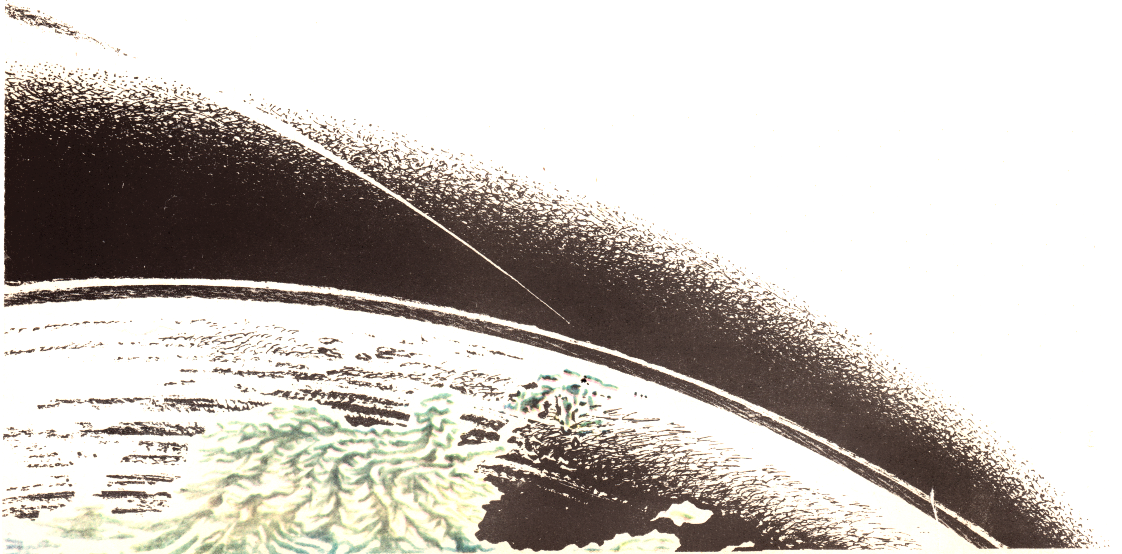
\includegraphics[width=\textwidth]{apogee1}

Продолжение. Начало см. «ТМ» № 8-12 за 1985 г. и № 1-2 за 1986 г.

Коршунов включил двигатель на двухстах километрах.

Это было намечено заранее. Орбита, получающаяся после прохождения атмосферы — так называемый тормозной эллипс,— необычайно чувствительна к самым небольшим изменениям скорости входа. Для малых судов, вроде нашего, важен и другой фактор: масса корабля из-за расхода топлива заметно уменьшается, и он потом тормозится сильнее. «Бывает выгоднее просто слить топливо,— рассказывал	Коршунов,— чем тормозить движком. Так иногда делают».

Надо учитывать, что атмосфера «дышит», ее плотность меняется в зависимости от времени суток и солнечной активности. Если корабль идет в атмосферу для посадки, это неважно: все маневры сдвигаются по высоте на несколько километров, и только. Но когда он, подобно «Кон-Тики», лишь задевает воздушную оболочку и снова уходит в космос, точная атмосферная сводка на данный момент столь же необходима, как прогноз погоды для авиаторов. Вот почему такие сводки — неотъемлемая часть космического радиовещания. «Главное — не увязнуть,— комментировал Коршунов нашу задачу.— «Кон-Тики» нельзя оставаться в атмосфере больше пяти минут. В баках тонна топлива, если жар подберется к нему, то конец».

«Кон-Тики» стремительно приближался к финишу. Заключительный отрезок пути — от геосинхронной орбиты до атмосферы — занял у нас около трех часов. Солнце все время пылало впереди, постепенно отодвигаясь от сверкающего края быстро растущего диска Земли. До планеты оставались считанные тысячи километров, когда траектория — скорость достигла уже десяти километров в секунду — начала выворачиваться параллельно горизонту. А за две минуты до перигея, на высоте 200 км, Коршунов спокойно развернул «Кон-Тики» днищем вперед и включил двигатель на десяток секунд; топлива на маневр ушло килограммов сто пятьдесят. Когда вес исчез, Коршунов возвратил «Кон-Тики» в прежнее положение. Мы лежали, наглухо привязанные к креслам, смотрели вперед и ждали. Бесконечное море блистающих облаков мчалось навстречу, в разрывах синел океан. Мы словно летели на высотном авиалайнере, практически горизонтально, но все- таки опускались — все медленнее и медленнее. А когда «Кон-Тики» пересек 80-километровую отметку, начались перегрузки.

Это продолжалось, как позже выяснилось, около двух минут. Сначала слабые, но быстро растущие, они рвали нас из кресел. Мы висели на ремнях над жаропрочным иллюминатором купола, ремни резали тело, перегрузка превысила единицу, потом двойку, «Кон-Тики» прессовал своей скоростью бесплотный воздух, тот накалялся, пылал, светился багровым цветом... Не помню, о чем я думал в эти секунды. Перегрузка достигла трех и начала падать. Мы были ниже семидесяти, но уже поднимались. Атмосфера отобрала у нашего кораблика часть скорости и теперь неохотно выпускала его из огненного плена... Потом снова стало легко.

— Высота? — деловито осведомился Коршунов, напоминая мне о моих штурманских обязанностях.

Я бросил взгляд на приборы.

— Восемьдесят!

— Скорость?

— Восемь с половиной!

— Отлично! — проговорил он, расстегивая ремни.— Мы сделали это, Саша, мы это сделали! Апогей будет у нас примерно две тысячи, как раз на орбите «Коперника». Полтонны топлива — и мы цепляемся за орбиту, остается еще столько же на маневрирование! Отлично, штурман, просто отлично!

Он искренне радовался, будто до последнего момента не был убежден, что все закончится столь успешно. На что тогда он рассчитывал? Однако спрашивать я не стал.

Коршунов поднялся из кресла, посмотрел вперед. Облака, до которых только что было рукой подать, быстро уходили вниз. На горизонте лежала тень — Солнце осталось сзади, мы приближались к линии терминатора.

Я посмотрел на своего командира. Лицо его выглядело смертельно усталым.

— Последний раз я проделывал такую штуку на Титане, в системе Сатурна,— сказал он.— Лет десять назад. Но там это проще, Саша. Скорости не те, да и атмосфера помягче.

Он вновь опустился в кресло, прикрыл глаза.

— Вздремну часок, что-то устал. Разбуди меня в апогее, штурман...

И он в самом деле заснул! Солнце позади нас опустилось за горизонт, «Кон-Тики» — впервые за несколько суток — окутал мрак. В небе зажглись звезды. Это была ночь, настоящая земная ночь, теплая, мягкая, человеческая! Подо мной, в нискольких сотнях километров, мирно спали люди. Неярко мерцали индикаторы. «Кон-Тики» поднимался все выше, стремясь к апогею орбиты. Коршунов не шевелился, я был совсем один, один под звездным небом. И вдруг...

Впереди засветилась изогнутая линия горизонта, из-за нее вынырнул маленький белый диск. Это восходила Луна. Луна, на камнях которой мы стояли всего неделю назад! Я смотрел на нее и чувствовал, как меня захлестывает неудержимой волной восторга.

Да, мы сделали это! Где ты, Эдик Рыжковский? На крохотной скорлупке прошли путь, на который даже свет тратит больше секунды! Мы прошли этот путь сами, без посторонней помощи, и не свернули даже после «Лагранжа», когда никто в мире не упрекнул бы нас за малодушие! «С берегов им кричали: — Вернитесь, друзья! — Но вперед они мчались, в чужие края — в решете по крутым волнам!»...

Я не замечал, как течет время. Луна поднималась все выше, она притягивала взгляд. Там остался Центр Королева, там шла по орбите станция «ЮГ», там, в точке либрации, уже работали ремонтные бригады, восстанавливая «Лагранж»... Все это было перед моими глазами, но я ничего не видел, слишком уж далеко. Но мы, мы-то были там так недавно!

Я посмотрел на приборы. Высота — около двух тысяч, вертикальная скорость уменьшилась почти до нуля, до апогея остались считанные минуты. Я перевел взгляд на командира «Кон-Тики». Его лицо, озаренное лунным светом, было безмятежно спокойным. Мне стало жалко его будить. Да и надо ли? Его действия при последнем маневре стояли у меня перед глазами. Я положил пальцы на клавиатуру. Осторожно — чтобы не потревожить Коршунова — развернул «Кон-Тики» днищем вперед. Луна исчезла из поля зрения, снова стало темно. Я включил двигатель, тот запел. Вновь появился вес — нормальная тяжесть, форсировать режим я не собирался. На душе было радостно и легко...

Не знаю, сколько это продолжалось— наверное, не больше минуты. - Чей-то вопль буквально потряс кабину, чья-то рука отшвырнула меня от пульта... Когда я очнулся, двигатель грохотал, кабину озарял яркий лунный свет, хищный профиль Лунного Коршуна нависал над пультом управления... Потом двигатель «Кон-Тики» захрипел и умолк, умолк навсегда.

Я был убит. Внутри — пустота, я уже знал: моя ошибка непоправима. Я включил двигатель в апогее; чтобы перейти на круговую орбиту, нужно было увеличить скорость судна на несколько сот метров в секунду. Я же сделал наоборот... Торможение, торможение — последние часы мы говорили только о торможении... Коршунов вновь увеличил скорость, но мы остались на эллипсе. Если перигей лежит за пределами атмосферы, тогда еще есть надежда. Если же нет...

Коршунов молча изучал показания приборов. Лицо его было непроницаемым.

— Тьма, Саша,— проговорил он тихо.— Помнишь, что я тебе рассказывал? Перигей будет там же, на тех же семидесяти. Это Тьма, штурман...

Словно споря с его словами, кабину затопили яростные потоки света — над горизонтом взошло Солнце. Впереди сверкали бесконечные поля облаков. Мы вновь падали в небо Земли — но топлива в баках не было, и не было в мире силы, способной остановить это падение!..

\subsubsection{МЯГКОЙ ПОСАДКИ!}
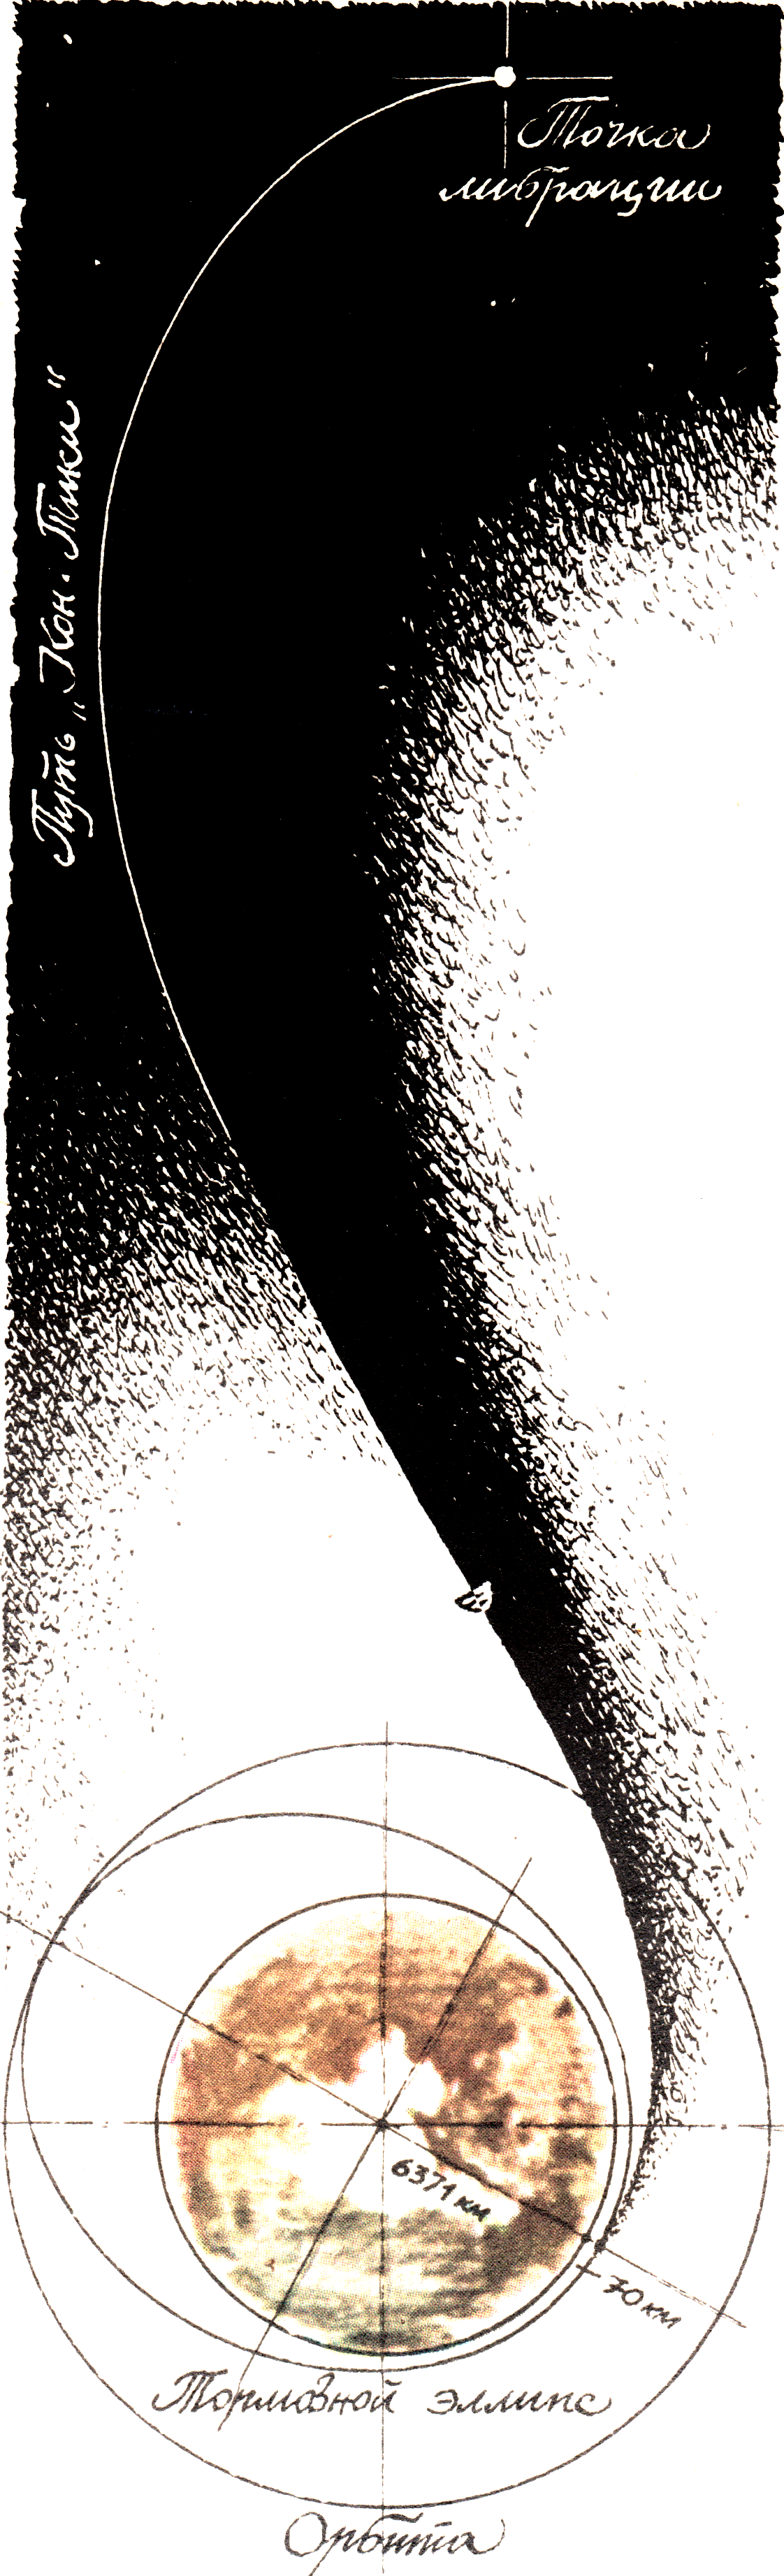
\includegraphics[width=0.5\textwidth]{apogee2}
Скажем без обиняков — ситуация заставляет вспомнить известную поговорку: «Если все идет хорошо, значит, вы чего-то не заметили». Под смертельной угрозой оказались не только цели полета, но и жизни его участников... Однако отступать поздно и некуда. Для повторения столь блистательно Начатой и так нелепо завершившейся операции (предварительное торможение, вход в атмосферу на второй космической скорости, аэродинамический маневр, переход на тормозной эллипс и маневрирование в апогее) предлагаем вашему вниманию программу «Атмосфера-1».

00.Сх 01.ИПА 02.+ 03.ПА 04.ИП7 05.- 06.Fx<0 07.13 08.ИПВ 09./-/ 10.$\div$ 11.БП 12.56 13.с/п 14.П8 15.П2 16.$\div$ 17.ИП6 18.x 19.ИПВ 20.Fx$^{2}$ 21. ИП0 22.Fx$^{2}$ 23.+ 24.П9 25.$\div$ 26.ИП7 27.ИПА 28.- 29.ИП3 30.$\div$ 31.9 32.+ 33. Fx<0 34.36 35.Сх 36.9 37.- 38.F10$^{x}$ 39.ИП1 40.x 41.- 42.ИПД 43.ИП8 44.- 45.Fx$\geq$0 46.00 47.ПД 48.ИП5 49.+ 50.$\div$ 51.ИП9 52.F$\sqrt{}$ 53.х 54.П9 55.ИП2 56.ИП9 57.ИПВ 58.ИПА 59.$\div$ 60.- 61. ИП0 62.х 63.х 64.ИП0 65.+ 66.П0 67.ПП 68.92 69.ИПА 70.$\div$ 71.Farcsin 72.ИПС 73.+ 74.ПС 75.\FO 76.ИП0 77.Fx$^{2}$ 78.ИП4 79.ИПА 80.$\div$ 81.- 82.ИПА 83.$\div$ 84.ИП9 85.ИПВ 86.х 87.+ 88.х 89.ИПВ 90.+ 91.ПВ 92.FBx 93.+ 94.х 95.2 96.$\div$ 97.в/о

Она предназначена для численного моделирования различных маневров космических аппаратов (взлет, выход на круговые и эллиптические орбиты, баллистический полет в атмосфере, снижение на парашютах, посадка) в непосредственных окрестностях планет, окруженных газовыми оболочками. Исходные данные частично совпадают с теми, что использовались в предыдущих программах: (текущее расстояние от центра планеты, м) ПА (вертикальная скорость, м/с) ПВ (узловое расстояние от какой-либо опорной точки, градусы) ПС (горизонтальная скорость, м/с) ПО (текущий запас топлива, кг)
ПД (гравитационная постоянная планеты, м$^{3}$/с$^{2}$) П4 (масса корабля без топлива, кг) П5 (скорость истечения продуктов сгорания, м/с) П6 (радиус планеты, м) П7. В регистр 3 засылается характерный масштаб атмосферы — высота (м), на которой плотность уменьшается в десять раз (предполагается, что она меняется по экспоненте). Наконец в регистр 1 вводится половина произведения плотности воздуха на нулевой высоте (кг/м$^{3}$) на площадь сопротивления космического аппарата (м$^{2}$). Последняя равна, в свою очередь, произведению площади миделевого сечения аппарата на коэффициент сопротивления. Судя по данным отчета А. Перепелкина, состоянию атмосферы в момент финиша соответствовало 17500 ПЗ; плотность воздуха на уровне моря составляет примерно 1,3 кг/м$^{3}$, площадь же сопротивления «Кон-Тики» при обдувании со стороны купола, если верить имеющимся в распоряжении редакции эскизам, была несколько меньше 10 м$^{2}$, так что в качестве достаточно хорошего приближения можно принять 5 П1.

Работа с программой «Атмосфера-1» начинается, как обычно, командой В/О С/П. При останове на индикаторе светится текущая высота полета в м, переменные хранятся в «своих» регистрах. Двигатель в данной программе ориентирован строго по вектору скорости (начальная скорость поэтому должна задаваться отличной от нуля); при его включении скорость увеличивается или уменьшается, но направления не меняет. Маневр задается командой: (расход топлива, кг) ПП (время, с) С/П (это соответствует разгону аппарата; для торможения перед С/П следует скомандовать ПП /—/). Если команда подана с превышением наличного запаса топлива, она, как всегда, блокируется. На внеатмосферном участке траектории не следует задавать время маневра больше 200 с; при полете в атмосфере, в условиях заметного аэродинамического торможения, целесообразно остановиться на значении 10 с. Посадка производится так же, как и при работе с программой «Лунолет-3». Переключатель Р-Г устанавливается в положение Г.

Программа «Атмосфера-1» позволяет и моделировать спуск космического аппарата на парашютах. Парашютная система задействуется при снижении скорости до 100-200 м/с; для этого достаточно, не меняя прочих параметров, увеличить площадь сопротивления (то есть содержимое регистра 1) в 10-1000 раз. Шаг по времени в момент раскрытия парашютов необходимо уменьшить до нескольких десятых долей секунды; рекомендуется также поэтапное увеличение площади сопротивления — это соответствует задействованию сначала тормозного парашюта, затем основных.

Структурно программа «Атмосфера-1» похожа на предыдущие. По адресам 04-07 производится вычисление текущей высоты полета и сравнение ее с нулем. Если высота положительна, то управление передается на адрес 13 (останов для ввода очередного маневра), если же отрицательна, то вступает в действие «посадочный блок» (08-12). Он организован точно так же, как в программах «Лунолет-3», «Маскон» и «ОС-1»: отрицательная высота делится на вертикальную скорость (которая при посадке, как правило, тоже отрицательна), знак перед получившимся числом меняется на противоположный, после чего оно используется в качестве времени очередного маневра с прежним ускорением. Легко видеть, что если последнее равно нулю или отрицательно (вертикальная скорость по мере приближения к поверхности постоянна либо увеличивается), то при повторении этой процедуры несколько раз ваш корабль вернется на нулевую высоту, а его скорость окажется такой же, как и в момент контакта с поверхностью (отметим, что при расчете высоты попутно происходит ее округление — до десятых долей метра, если радиус планеты измеряется тысячами километров). Если же вертикальное ускорение положительно (скорость корабля при снижении убывает), то посадочный блок «подбросит» аппарат на некую положительную высоту и, таким образом, своей задачи не выполнит (на это указывает в своем письме в редакцию москвич С. Вардин). Во избежание недоразумений лучше всего садиться с выключенным двигателем либо на малой тяге — более точный посадочный блок попросту не умещается ни в программу «Атмосфера-1», ни в «Лунолет-3» и «ОС-1».

При нормальном задании маневра расход записывается в регистр 8, время — в регистр 2, регистр 9 используется как рабочий, для временного хранения промежуточных результатов вычислений. Команды 16-54 рассчитывают сумму реактивного ускорения и аэродинамического торможения, затем к ним добавляются центробежное и кориолисово ускорение, после чего вычисляются новые значения координат и компонент скорости. Фрагмент (31-37) введен из-за несовершенства процедуры, с помощью которой ПМК вычисляет функцию 10$^{x}$: при отрицательных аргументах, превышающих по модулю 99, «Электроника» выдает вместо нуля сообщение ЕГГОГ. Рассматриваемый фрагмент устраняет эту неприятность, задавая на высотах свыше 150 км (для Земли) постоянную плотность, равную одной миллиардной доле плотности на нулевой высоте.

Из-за перегруженности счетного блока для преобразования радианов в градусы вместо применявшейся раньше точной последовательности 18O X F$\pi\div$ (6 команд) используется приближенная формула (71); она справедлива лишь при довольно малых (не более 10—20\degree) угловых перемещениях космического аппарата; по этой причине ограничения на шаг по времени не снимаются даже при полете по круговой орбите.

Концовка программы «Атмосфера-1» (92-97) одновременно используется в качестве подпрограммы (вызов 67-68); этот прием использовался и прежде. Время маневра, введенное в стек командой по адресу 55, переводится тремя последующими командами (56-58) в регистр Т, «цепляется» за конец стека и неоднократно используется в вычислениях (при умножении по адресам 63, 88 и дважды 94). Таким образом, экономится несколько ячеек программной памяти, отпадает необходимость записывать время в посадочном блоке.

Займемся очередным заданием — повторить маневры «Кон-Тики» в окрестностях Земли. Программа «Атмосфера-1», комплект исходных данных: 2200 П5 3660 П6 6371 ВП 3 П7 Fx$^{2}$ 9,81 Х П4 5 П1 17500 П3, регистры А, В, С, Д, 0 заполнить в соответствии с результатами выполнения предыдущего задания. Комбинируй ракетное и аэродинамическое торможение, обеспечить переход корабля на тормозной эллипс с апогеем 2000 км, после чего отработать оба варианта: 1) выполнить планировавшуюся операцию (выход на круговую орбиту высотой 2000 км) и 2) подготовиться к повторному входу в атмосферу по эллипсу с высотой в перигее 70 км (из-за вычислительных ошибок орбита, если оставить все как есть, пройдет в перигее вне атмосферы). Зафиксировать свои координаты и скорости на высоте 100 км и ждать следующего — судя по всему, последнего — выпуска. Посмотреть, как мог выглядеть финиш «Кон-Тики», если бы А. Перепелкин в свое время включил в заявку требование насчет парашютов.

\subsubsection{ОХОТА НА ИНОПЛАНЕТНЫХ ЧУДОВИЩ (3)}
Самым,- пожалуй, неприятным обитателем глубин нашего «числового океана» (см. предыдущие выпуски) является Тьма — при любом контакте с ней индикатор гаснет. Основные владения Тьмы располагаются между порядками 500 и 600 (таким образом, всякое число от 1 ВП 500 до 9,9999999 ВП 599 — это Тьма). Для первого знакомства с ней можно в режиме АВТ набрать на клавиатуре такую, например, последовательность команд: 1 ВП 70 Fх$^{2}$ (Е.ГГОГ) Fx$^{2}$ (ЗГГОГ) Fx$^{2}$. Индикатор гаснет — наши действия привели к числу 10$^{560}$, а это, конечно же, Тьма. Легко убедиться, что ПМК не отзывается теперь ни на один приказ с пульта. Однако если его выключить на несколько секунд, а затем включить снова, он будет работать как ни в чем не бывало.

Чтобы упрятать Тьму в «клетку» (адресуемый регистр), можно воспользоваться простой программой: 00.Fx$^{2}$ 01.Fx$^{2}$ 02.Fx$^{2}$ 03.ПА 04.Сх 05.С/П. Команда: F АВТ В/О 1 ВП 70 С/П. После останова на индикаторе горит ноль, но в регистре А сидит Тьма! Если вы рискнете и выпустите ее оттуда (ИПА), то индикатор погаснет, придется отключить калькулятор и вводить программу снова.

Как вы помните, для количественного анализа чудовищ 4-го этажа использовался ЗГГОГ из регистра 9. Однако для расшифровки как ОС-оборотней, так и Тьмы такой анализатор непригоден. Чтобы дешифровать Тьму (да и любые другие «суперчисла»), полезен логарифмический анализатор: 00.Fx$^{2}$ 01.Fx$^{2}$ 02.Fx$^{2}$ 03.Flg 04.1 05.0 06.0 07.0 08.— 09./—/ 10.П9 11.КИП9 12.\XY 13.ИП9 14.— 15.FBx 16.\XY 17.F10$^{x}$ 18.С/П. Программа логарифмирует сформированное командами (00-02) «чудовище» и вычисляет его мантиссу и порядок, так что после останова в регистре X оказывается мантисса (с небольшой ошибкой в последних десятичных знаках), в регистре Y — порядок. Обратите внимание на фрагмент (04-09) — вычисленный логарифм числа вычитается из тысячи; легко убедиться, что такая коррекция необходима при логарифмировании всех «сверхчисел», вплоть до Нуля (то есть по 9,9999999 ВП 799 включительно). Фрагмент (10-13) использует для выделения целой части числа команду косвенного вызова; как справедливо указывают в своих письмах Д. Кайков из Белгорода и другие читатели, это наиболее простой путь выполнения такой операции на «Электронике БЗ-34» (в новых моделях ПМК для нее предусмотрена специальная команда).

Испробуем наш анализатор на Тьме: В/О 1 ВП 70 С/П. После возведения в восьмую степень должно, очевидно, получиться число 10$^{560}$. На индикаторе зажигается приближенное значение мантиссы (1,0002303), в регистре Y оказывается совершенно правильная величина порядка (560).

Можно ли вызвать Тьму в регистр X? Казалось бы, странный вопрос... Но введите в ПМК программу: 00.Fx$^{2}$ 01.Fx$^{2}$ 02.Fx$^{2}$ 03.К7 (подойдет и любая другая «неправильная» команда, начинающаяся с К). Перейдите в режим АВТ и скомандуйте: В/О 1 ВП 70 С/П. На индикаторе загорается сообщение ЕГГОГ (результат «неправильной» команды), но под ним скрывается Тьма—если отдать сейчас одну из команд КНОП, Kl, К2, стрелка вверх (ввод в стек) или F АВТ, индикатор погаснет. Тьма, «замаскированная» сообщением ЕГГОГ, находится в регистре X, и с нею можно обращаться как с любым «нормальным» числом — умножить на что-нибудь, разделить, прологарифмировать вручную, используя приведенную выше процедуру... А что, если попробовать вычислить число, обратное Тьме? Команда: F 1/х. На индикаторе — ноль. Казалось бы, ничего удивительного — что же еще могло получиться в результате такой операции? Однако не будем спешить с выводами, заглянем в регистр С. ИПС ИПС. На индикаторе — знакомый по прошлому выпуску «хвост» (00,0000ЕЕ) оборотня, равного 10$^{440}$. Итак, разделив единицу на 10$^{560}$, мы получили 10$^{440}$; впрочем, если вспомнить, что наш «числовой океан» характеризуется периодом в 1000 по величине порядков, в этом опять-таки нет ничего удивительного: единица в «арифметике» ПМК тождественно равна 10$^{1000}$ (вспомните коррекцию логарифма, о которой только что шла речь). Отсюда следует важный вывод: числа, обратные Тьме, это ОС-оборотни; следовательно, числа, обратные ОС-оборотням,— это Тьма; значит, во избежание неприятностей не стоит производить над ОС-оборотнями такой операции... Кроме того, возникает подозрение, что в наш «числовой океан» можно проникнуть и с «черного хода» — через числа с отрицательными порядками; забегая вперед, укажем, что это действительно так.

Кроме своего «законного» этажа, Тьма занимает и две «ниши» в мире ОС-оборотней: от 1 ВП 450 до 9,9999999 ВП 469 (оборотни первого порядка) и от 1 ВП 445 до 9,9999999 ВП 446 (оборотни второго порядка); легко видеть, что в этих мирах Тьма «оккупирует» еще и соседний этаж, где, по идее, должны были бы располагаться С-ЕГГОГ- оборотни (числа с порядками между 600 и 700), с которыми мы познакомимся в следующем выпуске. Отдайте, например, такую команду (в ПМК введена последняя из приведенных программ, завершающаяся К7): В/О 1 ВП 58 С/П. На индикаторе — сообщение ЕГГОГ, под ним скрывается ОС-оборотень, равный 10$^{464}$. Нажимаем КНОП, на индикаторе ноль. ИПС — индикатор гаснет, Тьма...

Казалось бы, Тьму можно использовать лишь в электронных играх со «смертельным исходом»: записав ее в регистр, нетрудно добиться того, чтобы при ошибке со стороны играющего пришлось бы вводить программу заново. Однако это далеко не так, практические применения Тьмы гораздо шире. Они связаны с «тайными адресами» программной памяти «Электроники».

В прошлом выпуске рассказывалось о 160-шаговом цикле, которым характеризуется работа ПМК. В этот цикл входят все адреса, заканчивающиеся на какую-либо цифру. А куда передастся управление при команде перехода на адрес, завершающийся буквенным символом?

Отдайте в режиме АВТ, например, команду БП 0А и посмотрите, куда передалось управление. F ПРГ. Знакомая картина, индикатор гаснет, мы столкнулись с Тьмой... Отключите «Электронику» на несколько секунд, включите ее снова и повторите эксперимент: БП 0А. Только теперь перед F ПРГ нажмите ШГ влево и ШГ вправо. Казалось бы, ничто не должно измениться... F ПРГ. Справа горит 10, следовательно, управление передалось на этот адрес! Таким образом, «явному» адресу 10 соответствует «тайный» адрес 0А; самое важное — при работе по программе команды переходов по ним дают совершенно тождественные результаты.
«Тайные» двойники есть у многих адресов главной и побочных ветвей 160-шагового цикла. Адресу 11 соответствует 0В, 12-0С, 13—0Д, 14—0Е, 20—1А, 21—1В и так далее (рекомендуем составить для себя табличку «тайных» и «явных» адресов всех ветвей 160-шагового цикла). Это позволяет, в частности, использовать хранящиеся в регистрах буквенные сообщения в качестве адресов перехода при косвенной адресации. (Несколько слов о косвенных обращениях вообще: в регистры ПМК можно записывать не только числа, с которыми нужно работать, но и номера регистров, с содержимым которых мы собираемся что-то делать, или адреса переходов.)

Сформируйте, например, символ Е и зашлите его в регистры 9 и 0: 1 К7 (ЕГГОГ) ВП П9 П0. Отдайте теперь команду К БП 9. Управление должно перейти на адрес, хранящийся в регистре 9, а там у нас находится символ Е! Куда перейдет управление? Логично предположить, что на «тайный» адрес 0Е, которому, как мы уже знаем, соответствует «явный» адрес 14 основной
ветви программы. Действительно, если сделать ШГ влево, ШГ вправо, F ПРГ, убедимся, что это так. А что произойдет при команде К БП 0? Адрес, хранящийся в регистре 0, модифицируется (уменьшится на единичку), и управление перейдет на модифицированный адрес. Легко убедиться, что «модификация» в данном случае — это преобразование символа Е в Г, а управление передается на «тайный» адрес 0Д, которому соответствует «явный» 13... (К слову сказать, буквенные символы могут использоваться и при командах косвенного вызова и косвенной записи. Если сейчас, например, отдать команду КИП0, Г преобразуется в L, а на индикаторе появится содержимое регистра В.)

«Тайные» адреса, как и «явные», можно использовать и в качестве кодов команд. Читатели А. Морев из Устинова, М. Точин из Вологды и другие обратили, например, внимание на блок выдачи видеосообщений в программе «Лунолет-3» («ТМ» № 9 за 1985 год): 60.Fx<0 61.61 62.Fx$\geq$0 63.63 64.С/П. Как он работает? «Мой внук Артем Горин, ученик пятого класса, утверждает, что здесь используется то обстоятельство, что коды операций ИП1 и ИП3 совпадают с адресацией соответствующих условных переходов»,— пишет читатель Е. Григорьев из Москвы. Что ж, Артем совершенно прав. Находящееся в регистре X число сравнивается с нулем и, если условие по адресу 60 не выполняется, управление вторично передается на адрес 61. Эта комбинация цифр воспринимается теперь как код команды ИП1, и вызывается одно из двух видеосообщений. Оно, в свою очередь, сравнивается с нулем, благополучно проходит эту проверку (оба видеосообщения воспринимаются как положительные числа), и управление передается на команду останова С/П. Если же входное число меньше нуля, то оно переправляется на вторую проверку, естественно, не выдерживает ее, управление передается на адрес 63, эта комбинация воспринимается как код команды ИП3, вызывается второе сообщение и происходит программный останов. В результате экономятся две ячейки программной памяти: оба адреса перехода служат одновременно и командами вызова. Достаточно очевидно, что наличие «тайных» адресов расширяет возможности использования рассмотренного приема.

Как видим, охота на Тьму завершилась успешно: трофеи взяты немалые.

Михаил ПУХОВ

\subsection{SOS ПОСЛЕ ФИНИША}
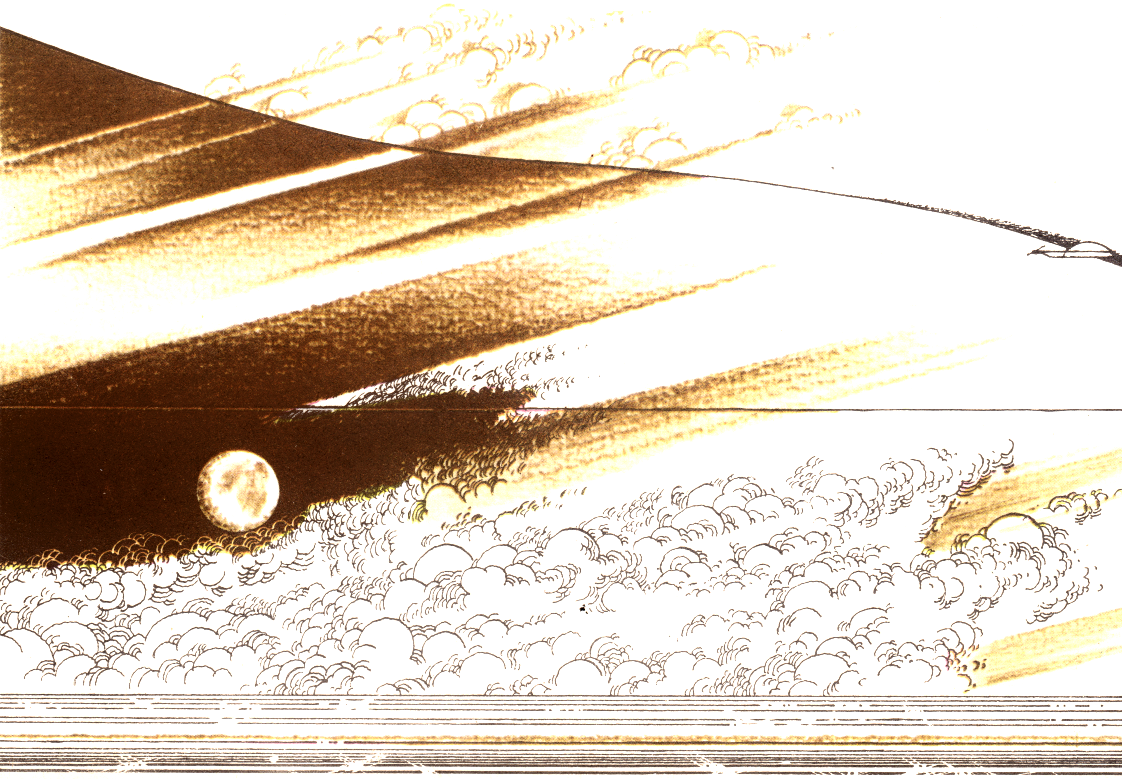
\includegraphics[width=\textwidth]{sos1}

Окончание. Начало см. «ТМ» «М 8-12 за 1985 г. и № 1-3 за 1986 г.

— Здесь станция «Коперник»,— повторил голос из динамика.— Станция «Коперник» к лунолету «Кон-Тики». Подтвердите заход на причаливание в восемнадцать ноль-ноль условного орбитального времени.— Последовала пауза, затем голос добавил уже другим тоном:— Телевидение беспокоится...

Коршунов зарычал и обрушил кулак на динамик. Тот умолк. До входа в атмосферу оставалось минут пять, не больше. Все было как тогда, в первый раз: бесконечные сверкающие поля облаков, в провалах — голубизна океана... Только теперь в баках «Кон- Тики» топлива не было; не было и самих баков, и це было двигателя — все это хозяйство, отстреленное полчаса назад, шло сейчас по собственной, отличной от нашей траектории, чтобы спустя несколько минут вспыхнуть падающей звездой в небе Земли...

Не было ни паники, ни упреков. «Это стандартная машина, штурман,— сказал Коршунов.— Днище кабины отделено от двигательного отсека толстым слоем теплозащиты. Будем надеяться, на торможение ее хватит. А если прогар — так это мгновенно, ты знаешь...»

«А потом?» — спросил я. «Если не будет прогара в самом начале,— сказал он,— останется одна опасность — посыпаться в самом конце. Не будем об этом думать. Там, в перигее, океан. Наша задача — выйти в горизонтальный полет на нулевой высоте и на минимальной скорости. Это наш шанс...»

Потом последовал отстрел двигательного отсека. Мы молча наблюдали, как блистающий барабан, медленно кувыркаясь, уходит в черноту космоса. Я четко себе представлял, хотя не мог этого видеть, как преобразился сейчас «Кон-Тики» — стал вдвое ниже, превратился в приплюснутый диск, увенчанный сзади хвостовым оперением. Да, оно пригодилось. Корабль походил сейчас на бескрылый маленький самолет. Только скорость его была на два порядка больше...

Облака надвигались, пора было разворачивать «Кон-Тики» днищем вперед, но Коршунов медлил, молча глядя на простирающийся перед нами пейзаж. «В последний раз»,— сказал я себе мысленно, но сам себе не поверил. Нет, это невероятно. Герои Жюля Верна и Герберта Уэллса уже прошли по этому пути, а когда это было?! «Как птицы, штурман, как птицы!» — вспомнил я. Нет, мы еще поборемся!

Коршунов развернул «Кон-Тики» на высоте сто километров. Микродвигатели ориентации сработали четко. К счастью, они располагались на основании кабины, не были связаны с двигательным отсеком. Теперь мы не видели ничего, кроме звездного неба: лежали в креслах — голова вниз, ноги вверх — и ждали. Прошла минута — мы уже снизились до 80 км, приближаясь к перигею орбиты. Внезапно я почувствовал под собой кресло. Атмосфера тормозила «Кон-Тики» все сильнее и сильнее — еще минута, и я ощущал уже нормальную земную тяжесть.

— Высота? — спросил Коршунов.'

— Семьдесят!

— Скорость?

— Восемь!

— Скорость спуска?

— Сто метров!

— Сейчас начнется! — прокричал он.— Держись, штурман!

Предупреждать меня не было нужды.

Перегрузка увеличивалась. Двигатели ориентации удерживали «Кон-Тики» строго перпендикулярно потоку. Я не отрывал взгляд от альтиметра. Высота 65 км, скорость 7 км/с, скорость спуска — по-прежнему 100 м/с. Перегрузка достигла полутора единиц и продолжала расти. Еще полминуты. Высота 60, перегрузка стала трехкратной, скорость уменьшилась до шести километров в секунду. Корабль окончательно увяз в атмосфере. Путь оставался один — вниз, только вниз!

— Скорость спуска?

— Двести,— ответил я, с трудом ворочая языком.

— Много,— услышал я голос Коршунова. Небо за фонарем дрогнуло — он изменил угол атаки, чуть-чуть, градусов на десять, наклонив «Кон-Тики» вперед. Появилось вертикальное ускорение, спуск начал замедляться. Высота пятьдесят пять километров, скорость — чуть больше пяти километров в секунду. Перегрузка перевалила за тройную и вдруг стала ослабевать. Я почувствовал это сразу. Режим поддержки — из-за наклона судна появилась подъемная сила, мы практически перешли в горизонтальный полет, плотность воздуха оставалась постоянной, и наша скорость неуклонно уменьшалась. Вместе с ней уменьшались сила сопротивления и перегрузка.

— Скорость?

— Три с половиной.

— Высота?

— Пятьдесят пять...

Перегрузка падала. «Кон-Тики» все сильнее наклонялся вперед. Теперь его удерживали стабилизаторы. Мы медленно снижались, скорость убывала. На высоте 40 км она составляла уже всего полтора километра в секунду. «Кон-Тики» шел в режиме парашютирования, под углом 45 градусов к потоку, скорость спуска была умеренной, меньше ста. Возвратилась земная тяжесть.

— Вот и все, Саша! — В голосе Коршунова послышалось торжество.— Самое страшное позади, теплозащита выдержала. Значит, мы победили!..

И он поднялся из кресла. Да, все было позади, я это понял. Понял по- настоящему! Отнюдь не исчезновение перегрузки было причиной тому огромному облегчению, которое я почувствовал... Мы летели уже не в космосе, а в атмосфере, на «самолетной» высоте и с «самолетной» скоростью. В том, что Коршунов благополучно посадит «Кон-Тики», я не сомневался. Фактически мы были уже дома!..

— Иди сюда, штурман,— позвал он. И подмигнул: — Ракетой ты уже управлял, и весьма удачно. Попробуй теперь, что такое полет в атмосфере. Чтобы не было никаких обид.

Я занял его место и бросил взгляд на приборы. Высота 30 км, скорость — ровно километр в секунду. Ярко светило Солнце, облака были внизу, мы шли практически горизонтально. Коршунов стоял рядом с креслом, придерживаясь за спинку.

— А что надо делать?

— Держать угол атаки,— пояснил он.— Чем он больше, тем больше подъемная сила, но и сопротивление тоже. Четыре градуса, думаю, будет вполне нормально. Вот этот рычаг видишь? Уверяю тебя, это нетрудно.

Пульт перед его креслом был точно такой же, как мой, с одним-единственным дополнением. После моего поединка с «роботом-бюрократом» здесь появилась новая шкала: «Угол атаки». И рычажок, перемещающийся вдоль шкалы, и цифры от нуля до девяноста...

Я передвинул рычажок назад, к цифре 4. Он поддался легко, без сопротивления. «Кон-Тики» послушно качнулся вперед, приняв почти горизонтальное положение.

— Так держать, штурман! — сказал Коршунов. Он был очень доволен.— Так держать!

Собственно, ничего от меня не требовалось. Передвинул рычаг — и только. Произошло при этом, насколько я понимаю, следующее. Команда с пульта поступила на какой-то микропроцессор, тот сравнил ее с информацией от внешних датчиков, передал на серводвигатели тормозного щитка управляющий сигнал... В результате судно приняло нужную ориентацию относительно набегающего потока. Но подъемной силы теперь не хватало, траектория загибалась вниз, вместе с ней наклонялся вперед корабль, скорость спуска, только что бывшая нулевой, увеличивалась. Пятьдесят метров в секунду, сто, сто пятьдесят... Все-таки плотность на этой высоте была еще ничтожной, поддержки недоставало, мы входили в крутое пике. Впереди, совсем рядом, белели облака, «Кон-Тики» мчался к ним словно пикирующий бомбардировщик, под углом градусов пятнадцать к горизонту. Высота быстро уменьшалась — двадцать пять километров, двадцать три, двадцать...

«И сколько так будет продолжаться?» — спросил я себя. Ответ подсказало кресло: надавило на меня с новой силой. Плотность за бортом увеличивалась, «Кон-Тики» наткнулся на эти более плотные слои и среагировал незамедлительно: сам, совершенно самостоятельно, выходил из пике. И перегрузка усилилась — меня уже ощутимо вдавливало в кресло. Полтора, наверное, не меньше.

— Довольно,— сказал Коршунов.— Вставай. С чужого коня...

Я до сих пор не знаю, что произошло. То ли я, отвлекшись на его голос, чуть изменил положение рычажка. То ли, что более вероятно, мы напоролись на какую-то локальную турбулентность, ничтожную флуктуацию плотности. Как бы то ни было, «Кон-Тики» сильно тряхнуло, послышался грохот падающего тела...

Он не устоял на ногах. Никто бы не устоял при таком толчке. И он упал. Упал при двойной перегрузке. Когда-то я читал фантастический роман о жизни на тяжелой планете, в условиях повышенной гравитации. Самое страшное для ее обитателей было — упасть. Падение означало смерть.

Я не сразу осознал, что случилось.

— Михаил! — с трудом крикнул я.— Ты что, Михаил?!

Ответом мне было молчание. «Кон-Тики», наткнувшись на плотные слои атмосферы, выходил в горизонтальный полет. Высота 13 км. Скорость — семьсот метров в секунду. Две с половиной тысячи километров в час...

«Кон-Тики» мчался над верхней границей облачности. Теперь я чувствовал нормальную тяжесть. Я повернул голову. Он лежал на полу. Недвижимый, бездыханный.

— Михаил! — заорал я.

Он не шелохнулся. «Кон-Тики» несся горизонтально, быстро теряя скорость. Шестьсот метров в секунду, пятьсот пятьдесят... Рычажок атмосферного пульта стоял в прежнем положении. Угол атаки — четыре градуса. Было жарко, на лбу выступил пот. Я весь обливался потом. Попробовал встать из кресла...

Не тут-то было. «Кон-Тики» — скорость снизилась уже до пятисот метров в секунду — вновь клюнул носом вниз. Я снова увидал облака. Мы входили в новое, еще более крутое пике. Все вокруг заволокло туманом. Скорость спуска росла, высота падала, пике становилось все круче.

Облака ушли вверх. Под собой я увидел бесконечный простор океана. Далеко впереди темнел массив какого-то континента. Кресло вновь давило снизу, «Кон-Тики» пытался выйти и из этого пике. Высота — шесть километров. Скорость — четыреста метров в секунду. Угол пикирования — около двадцати градусов к горизонту. Но он уменьшался, траектория становилась все более пологой. На что я надеялся? Что она окончательно выправится над самой морской поверхностью?..

Нет, из этого пике наш кораблик выйти не смог. На четырех километрах угол пикирования стабилизировался — около пятнадцати градусов. Но скорость медленно падала: 340 м/с, 320, 300... Я уже знал, что делать. «Наша задача — выйти в горизонтальный полет на нулевой высоте. Это наш шанс...»

Я весь обливался потом. Высота уменьшалась быстро, скорость, к сожалению, медленнее. На полутора километрах она упала до 250 м/с, до поверхности океана оставалось секунд двадцать, не больше. Она была гладкая, без морщинки. Штиль... «Кон-Тики» вновь начал заваливаться в крутое пике.

До воды оставались считанные сотни метров, когда я стал отжимать рычажок от себя: пять градусов, шесть, семь... Мы вышли на горизонталь на высоте двадцать пять метров. Скорость «Кон-Тики» была двести метров в секунду. Я осторожно увеличивал угол атаки, задирая судно носом кверху: восемь градусов, десять, двенадцать... Скорость уменьшалась, и высота тоже: девять метров, семь, пять... «Кон-Тики» несся над самой поверхностью, едва не касаясь воды. Сто двадцать метров в секунду, сто десять, сто... Сто, девяносто, восемьдесят! Я удерживал его под углом сорок пять градусов — максимум подъемной силы,— только скорости уже не хватало, и мы рухнули вниз!..

...Но падать нам было некуда — под нами была вода. Толчок был сильным, я удержался в кресле каким-то чудом. Раздалось оглушительное шипение, вверх взметнулось густое облако пара и, видимо, облако брызг. Но наше суденышко еще летело вперед — оно выскочило из этого облака, оставило его позади! И неторопливо замедляло ход, осваиваясь в новой среде...

Я повернул голову. Коршунов сидел на полу кабины, по лбу стекала узкая струйка крови. Взгляд его был странным. Раньше он никогда так на меня не смотрел.

— Ты хорошо сел, мальчик,— сказал он.— Не зря был чемпионом...

Не знаю, что он хотел этим сказать. Но переспрашивать я не стал.

* * *

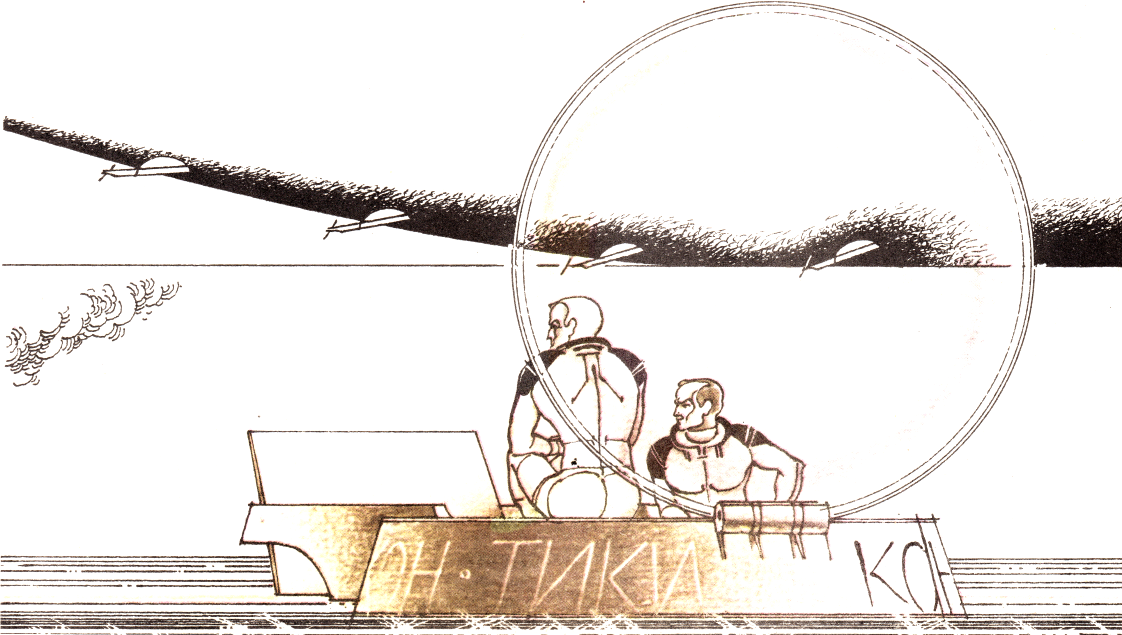
\includegraphics[width=\textwidth]{sos2}

— Надо как-то выкручиваться,— произнес он полчаса спустя. Прозрачная крышка была откинута, кругом был безбрежный синий простор, сверху — белые облака. Нас обдувал слабый ветерок. Мы сидели, подставив голые спины земному солнцу, и дышали земным воздухом, ни с чем не сравнимым.— Я вижу единственный выход.

— Какой?

— SOS,— коротко объяснил он.

— SOS? — Мне показалось, что я ослышался.— После всего, что мы сделали? Да тут до суши всего километров двести, от силы триста.

— И что ты предлагаешь? Вплавь? Думаешь, я умею плавать?

— Зачем же вплавь? Судно прекрасно дойдет своим ходом. Ветер хоть и слабый, зато попутный. Сутки-другие — и войдем в чьи-нибудь территориальные воды...

— Ну нет! — заявил командир «Кон-Тики».— Я, в конце концов, космонавт, а не капитан дальнего плавания. Врубай SOS, штурман, SOS на полную громкость!..

КОНЕЦ

\subsubsection{мягкой ПОСАДКИ!}
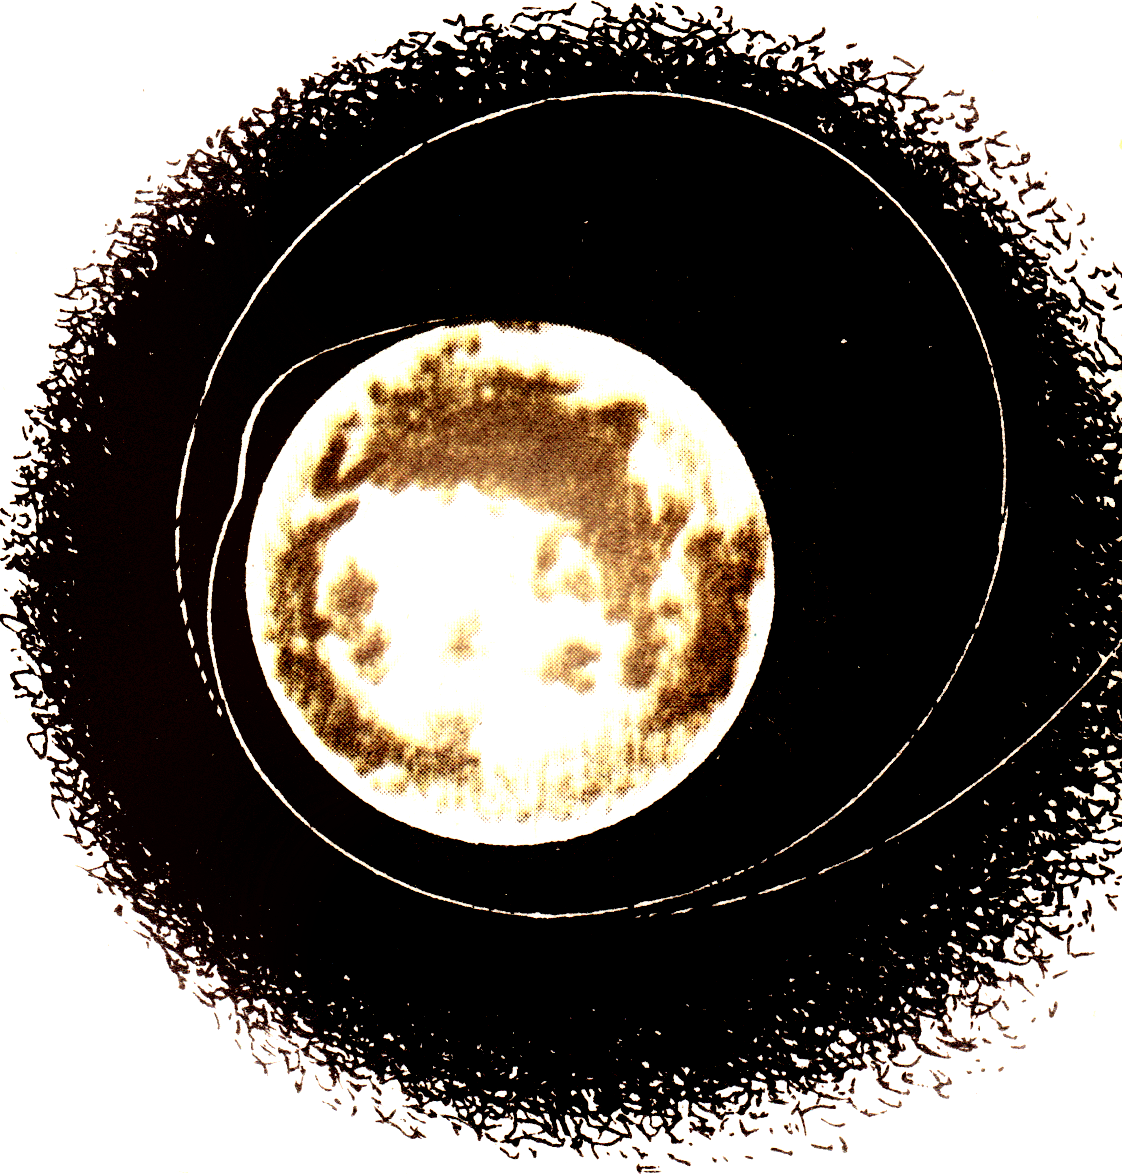
\includegraphics[width=0.5\textwidth]{sos3}

Конец венчает дело — традиционный заголовок раздела приобрел долгожданное содержание. Последний «переплет Перепелкина» (по выражению читателя М. Рыжкова из Новосибирска), как видим, завершился если не полной победой, то вполне достойным сигналом бедствия. К сожалению, в распоряжении редакции не имеется ни одной сколько-нибудь приличной программы, обеспечившей бы дальнейший путь «Кон-Тики» к земле (в том смысле, какой вкладывают в это слово моряки). Возможно, экипажу поможет кто-нибудь из читателей? А для посадки предлагаем вашему вниманию новую игровую программу «Атмосфера-2»:

00.Сх 01 ИПА 02.+ 03.ПА 04.ИП7 О5.- 06.Кх<o9
07.ИПВ 08./-/ 09.$\div$ 10.П2 11.ИП9 12.с/п 13.БП
14.57 15.П8 16.с/п 17.П2 18.Fcos 19.FBx
20.Fsin 21.ПД 22.ИП6 23.x 24.x 25.П5
26.FВх 27.ИПД 28.x 29.1 30.+ 31.ИП1 32.ИП8
33.ИП3 34.$\div$ 35. F10$^{x}$ 36.$\div$ 37.ИПВ 38.Fx$^{2}$
39.ИП0 40.Fx$^{2}$ 41.ПД 42.+ 43.F$\sqrt{}$ 44.x 45.х
46.П8 47.FBx 48.ИП5 49.x 50.ИПД 51.F$\sqrt{}$
52.$\div$ 53.ИПА 54.F1/x 55.+ 56.П5 57.ИП0
58.ИП8 59.ИПВ 60.ИП5 61.х 62.+ 63.x
64.ИП2 65.х 66.- 67.П0 68.ПП 69.92
70.ИПС 71.+ 72.ПС 73.ИПД 74.ИП5 75.x
76.ИПВ 77.ИП8 78.x 79.- 80.ИП4 81.ИПА
82.Fx$^{2}$ 83.$\div$ 84.- 85.$\uparrow$ 86.ИП2 87.x 88.ИПВ
89.+ 90.ПБ 91.FBx 92.+ 93.ИП2 94.x
95.2 96.$\div$ 97.в/о

Она предназначена для численного моделирования управляемого полета в атмосфере безмоторных летательных аппаратов (дельтапланов, космических кораблей многократного использования, детских бумажных голубей и «Кон-Тики»). Кое-какие исходные данные «унаследованы» от «Атмосферы-1» (см. предыдущий выпуск): (начальное расстояние от центра планеты, м) ПА (начальная вертикальная скорость, м/с) ПВ (начальная горизонтальная скорость м/с) ПО (радиус планеты, м) П7 (гравитационная постоянная планеты, м$^{3}$/с$^{2}$) П4 (характерный масштаб атмосферы, м) П3. В регистр 1 вводится половина произведения площади сопротивления аппарата (м$^{2}$) при нулевом угле атаки (когда днище «Кон-Тики» ориентировано параллельно потоку) на плотность воздуха на нулевой высоте (кг/м$^{3}$), разделенная на массу аппарата (кг). Цифры, которыми изобилует последняя часть отчета, склоняют к предположению, что данная константа составляла примерно 7,5 ВП /—/ 5 П1. В регистр 6 вводится отношение максимальной силы сопротивления (когда днище перпендикулярно потоку) к минимальной; из тех же цифр и имеющихся эскизов удалось оценить этот коэффициент в 30 П6. Наконец, в регистр С записывается начальное расстояние (м) от какой-либо опорной точки, в регистр 9 — сигнал о посадке Е15:115 К — (ЕГГОГ) ВП П9. Такой необычный шифр выбран потому, что он используется и как адрес условного перехода в команде Кх<о9, записанной по адресу 06. Переход в командах косвенной адресации (она в данном случае применена просто для экономии программной памяти) производится на адрес, совпадающий с двумя последними цифрами записанного в регистре числа: вместо Е15 можно использовать, например, Е115 или просто 151515 (читатели С. Аветисов из Еревана, В. Агафонов из Таганрога, Д. Горелин из Киева указывают, что на БЗ-34 первых выпусков невозможно формировать буквенные сообщения, по крайней мере, с помощью нормальной процедуры, используя ЕГГОГ и ВП; что ж, обладателям подобных моделей придется воспользоваться числовым сообщением).

При формировании шифра Е15 вместо команд КСх и К7 использована К-; это связано с вопросами читателей, приобретших «Электронику МК-61», в которой кое-что добавлено по сравнению с БЗ-34 и МК-54. «Неправильных» команд, начинающихся с К, в новом ПМК осталось всего три: со знаками вычитания, деления и умножения (В. Николайчук из Воронежа сообщил, что команды К1 и К2, как и в МК-54, выполняют функции «пустых»). Шестиклассник Е. Агеенко из Ульяновска информирует и о кое-каких новых способах получения видеосообщений на МК-61 с помощью команды К Инв; еще будет время о них рассказать. Восьмиклассник С. Лаптев из Брянска спрашивает:	стоит ли приобретать МК-61? «Зачем он мне, если к нему не подойдут ваши программы?» Отвечаем: приобретать стоит, наши программы к нему подойдут.

При полете в атмосфере, кроме сил, к которым участники рейса привыкли (гравитационная, центробежная и кориолисова), на аппарат действуют еще две: сила лобового сопротивления и подъемная сила. Первая направлена вдоль траектории, против вектора скорости; вторая — перпендикулярно. Обе зависят от плотности воздуха и скорости и меняются в зависимости от ориентации аппарата. Лобовое сопротивление минимально, когда угол атаки равен нулю (днище аппарата ориентировано вдоль потока), и максимально, когда он составляет 90\degree (поток бьет в днище). Подъемная же сила в этих крайних ситуациях отсутствует: она максимальна при промежуточном угле атаки 45\degree. Кроме того, она положительна при положительных углах атаки и отрицательна при отрицательных (например, если бы «Кон-Тики» перевернулся вверх днищем и тормозился в этом положении). Во избежание недоразумений укажем, что задача решалась приближенно, в пренебрежении тонкими аэродинамическими эффектами.

Работа с «Атмосферой-2» начинается командой В/О С/П. Переключатель Р—Г устанавливается в позиции Г. При останове на индикаторе загорается текущая высота полета (она же находится и в регистре 8), переменные располагаются в прежних ячейках. В регистр У выводится чрезвычайно важная (особенно при посадке) величина: полное вертикальное ускорение аппарата в м/с , если оно близко к нулю, скорость спуска практически не меняется.

Маневр задается командой: (время, с) ПП (угол атаки, градусы) С/П. Время в отличие от «ракетных» программ разрешается задавать равным нулю (штурманский режим): это дает возможность определить вертикальное ускорение при данном угле атаки без изменения остальных переменных (в реальном полете пилот эту величину попросту ощущает всем телом). При полете в атмосфере рекомендуется задавать время маневра не больше 5-10 с, а при заходе на посадку и того меньше. Позволяет «Атмосфера-2» осуществить и спуск на парашюте. Регистр 6 при этом следует обнулить, содержимое регистра 1 увеличить в 100-1000 раз, время маневра в момент раскрытия парашютов уменьшить до десятых долей секунды.

При контакте с поверхностью на индикаторе загорается сигнал Е15, при его появлении следует нажать С/П. Загорание нуля после одного или нескольких Е15 означает, что посадка завершена. В некоторых случаях летательный аппарат может «срикошетировать»: на индикаторе вновь зажигается положительная высота; значит, нужно продолжать полет. Посадка считается удовлетворительной, если горизонтальная скорость не превышает 100, вертикальная — 5 м/с.

Структурно программа построена аналогично предыдущим. Команды (01-05) вычисляют текущую высоту полета; если она отрицательна, то задействуется стандартный посадочный блок (07-14): вычисляется и записывается в регистр 2 отрицательное время возврата, из регистра 9 вызывается сигнал Е15, происходит останов для его индикации, а после нажатия С/П управление передается на начало блока решения уравнений движения (57). Если же высота положительна, то она записывается в рабочий регистр 8 и происходит обычный останов (15-16). Введенное с пульта время маневра записывается в регистр 2 (17), команды (18-30) вычисляют тригонометрические функции угла атаки, необходимые для расчета аэродинамических ускорений, последние суммируются с центробежным, кориолисовым и гравитационным, получившиеся дифференциальные уравнения численно интегрируются по формулам равноускоренного движения. Особых «тонкостей», кроме использования сигнала Е15 в качестве адреса перехода, в программе нет. Регистры 5,8 и Д служат рабочими ячейками для хранения промежуточных результатов вычислений. Концовка программы (92-97) работает и как подпрограмма (вызов 68-69). Горизонтальная скорость, введенная в стек командой (57), в результате команд (58-60) оказывается в регистре Т и используется в вычислениях по адресам 63, 66 и при сложении в первой команде подпрограммы. Стоит обратить внимание на команду (85): в расчетах она не нужна, ее назначение — сохранить величину вертикального ускорения в регистре Y. Отметим, что командой (52) производится деление на модуль горизонтальной скорости; по этой причине для расчета чисто вертикального спуска «Атмосфера-2» не годится.

«После появления на страницах журнала рубрики «Клуб электронных игр» сразу же купил ПМК,— пишет А. Горелов из поселка Тисуль Кемеровской области.— Но при наборе программы легко сделать ошибку. Чтобы убедиться, что программа набрана правильно, предлагаю печатать в конце каждой «проверочную задачу», а также значения всех переменных с точностью до последней цифры». Пожелание вполне разумное, охотно идем навстречу. Вот как мог выглядеть финиш «Кон-Тики» после выхода в горизонтальный полет. Исходные данные: 6371 ВП 3 П7 Fx$^{2}$ 9,81 Х П4 17500 ПЗ 7,5 ВП /—/ 5 П1 30 П6 115 К- (ЕГГОГ) ВП П9 ИП7 25 + ПА 200 П0 Сх ПВ ПС. В/О С/П — на индикаторе загорается высота 25. Приводим запись команд А. Перепелкина в виде: время/угол (показание индикатора). 5/6 (19) 5/8 (10,6) 5/10 (8,9) 5/12 (5) 5/18 (4,2) 5/24 (0,1) 1/45 (Е15). Есть контакт! С/П (Е15) С/П (Е15) С/П (0). Смотрим остальные переменные: ИП0 (77,749524) ИПВ (—3,4853011) ИПС (4272,5669).

Задание на этот раз очевидно: закончить путешествие. Комплект исходных данных тот же, что и в приведенном тесте, только регистры А, В и 0 нужно заполнить в соответствии с результатами предыдущей операции (тем, кто ее не выполнял, можем предложить такие цифры: ИП7 1 ВП 5 + ПА 8400 П0 280 /—/ ПВ Сх ПС). Рекомендациям, содержащимся в последней части отчета А. Перепелкина, -следовать можно, но вовсе не обязательно: путей в атмосфере много, и все они ведут вниз. Мягкой посадки!

Михаил ПУХОВ

\subsubsection{ОХОТА НА ИНОПЛАНЕТНЫХ ЧУДОВИЩ (4)}
Рейс «Кон-Тики» завершен, пора заканчивать и знакомство с глубинами «электронного океана». Но сначала ознакомимся с одной особенностью БЗ-34 (МК-54). «Занимаясь с микрокалькулятором,— пишет Д. Козьминский из г. Рубцовска Алтайского края,— я заметил интересную возможность увеличить число регистров памяти. Может, это и не открытие, но в качестве ячеек можно использовать и знаки арифметических действий, а также \XY и стрелку вверх (ввод в стек). Однако последняя спарена с «+», то есть эти дополнительные регистры работают как один».

Прав ли читатель? И да и нет. Легко убедиться, что клавиши «+»,	«—», "Х", «$\div$» и «\XY» при командах записи, вызова и переходов выполняют в точности те же функции, что и команды «0», «1», «2», «3» и «4», вплоть до совпадения кодов получающихся команд. Так, команда П+(код 40) тождественна П0 (тот же код), поэтому о каком-то расширении возможностей ПМК за счет этих «новых» команд говорить нельзя (в некоторых игровых программах, правда, можно для наглядности отдавать с пульта команды типа БП $\uparrow \pm$ С/П для перемещения по вертикальной координате и БП \XY $\pm$ С/П для перемещения по горизонтальной; с таким вводом мы скоро встретимся). Но Д. Козьминский прав в том смысле, что адресуемых регистров в памяти БЗ-34 вовсе не 14, как утверждается в заводской инструкции, а 15 — имеется еще один буквенный регистр Е: на клавиатуре ему соответствует стрелка вверх (ввод в стек). Нетрудно проверить, что по этому регистру можно осуществить полный набор команд (прямые запись и вызов, а также косвенные: запись, вызов, обращение к подпрограмме и переходы — четыре условных и один безусловный). Эти команды имеют собственные коды, (все они завершаются буквой Е) и исправно выполняются как при ручных вычислениях, так и при расчетах по программе. Лишь одна особенность отличает регистр Е от остальных: он постоянно связан с регистром 0! Иными словами, содержимое обоих регистров всегда совпадает.

Казалось бы, что толку от такого дополнительного регистра? Какая разница, 0 или Е, если числа в них все равно одинаковы? Действительно, команды прямой записи и прямого вызова по этим регистрам, несмотря на то, что коды их отличаются (40 и 4Е, 60 и 6Е), абсолютно взаимозаменяемы. А вот при косвенном обращении к регистру Е (как и к другим буквенным, а также «старшим» цифровым регистрам 7, 8 и 9) не происходит «модификации» находящегося в нем числа — оно, попросту говоря, не меняется; соответственно остается прежним и содержимое регистра 0. При косвенном же обращении к регистру 0 его содержимое «модифицируется» (уменьшается на единичку, как и в случае регистров 1, 2 и 3) — соответственно меняется и число в регистре Е. Эту постоянную связь удобно использовать в циклах по регистру 0 (см., например, простенькую программу «Мультфильм» № 12 за 1985 год; предоставляем читателям самим разобраться в том, как она работает). К слову сказать, в МК-61 связь Е—0 разорвана, поэтому обладателям этого ПМК придется в некоторых ситуациях искусственно ее вводить, что потребует минимум двух команд ИП0 ПЕ. Все такие случаи будут в дальнейшем оговариваться особо.

Столь обширное отступление потребовалось потому, что обитатели 7-го этажа «электронного океана», С-ЕГГОГ-оборотни, позволяют устанавливать подобную (правда, одностороннюю) связь между регистром С и любым другим. Введите в регистр С какое-нибудь число, например, 22, перейдите в режим ПРГ, наберите стандартную «водолазную» программу: 00.Fx$^{2}$ 01.Fx$^{2}$ 02.Fx$^{2}$ 03.ПА 04.Сх 05.С/П, вернитесь в режим АВТ и скомандуйте, допустим, 1 ВП 80 В/О С/П. На индикаторе 0, но в регистре А сидит С-ЕГГОГ-оборотень. ИПА. На индикаторе — 22, содержимое регистра С! Это главное свойство «сверхчисел» с порядками между 600 и 700 (сейчас в регистре А записано 10$^{640}$) — при их вызове в регистр X сами они тут же «отступают» в регистр Y, вытаскивая на индикатор число из регистра С (почему именно этому буквенному регистру такое предпочтение, никому не известно). С числом, которое горит сейчас на индикаторе, можно осуществлять различные операции. Например, 2 X (44) 4 $\div$ (11) 1 — (10) 15 + (25) F$\sqrt{}$ (5) F 1/х (0,2) и т. д. Но в регистре Y по-прежнему находится «сверхчисло». Попробуем \XY. На индикаторе вновь появляется 22 — «чудовище», вызванное в регистр X, незамедлительно отползло в свою «пещеру» (регистру Y), прикрывшись «добычей» (содержимым регистра С)...

Если нажать теперь знак сложения, после томительной паузы на индикаторе появится сообщение ЕГГОГ. «Сверхчисло», замаскированное под ним, собственной персоной явилось на индикатор! Это легко проверить, например, отдав команду Flg: на экранчике загорится 359,99998 — логарифм «сверхчисла» (с учетом периода в 1000 по величине порядков).

С-ЕГГОГ-оборотни обладают и многими другими, еще не вполне понятными свойствами. Использование их в электронных играх проблематично. Однако знать о них надо — с этими числами легко случайно столкнуться в районе отрицательных порядков (если, скажем, подать на вход «водолазной» программы число 1 ВП /—/ 45, то получится вовсе не ноль, как можно было предположить, а то самое, «сверхчисло», с которым мы только что познакомились; для ПМК нет разницы между 10$^{640}$ и 10$^{-360}$ —порядки отличаются ровно на тысячу.).

Сказанное относится и к числам с положительными порядками от 700 до 800 (соответственно с отрицательными между -200 и -300). Для знакомства с ними пригодится ЗГГОГ-анализатор: 1 ВП 50 Fx$^{2}$ Fx$^{2}$ П9 Сх. Подадим на вход «водолазной» программы, допустим, 1 ВП 90 В/О С/П. На индикаторе 0. ИПА. На экранчике появляется нечто несообразное (00,10000000 2). Это «длинный монстр», типичный обитатель данного этажа. Справиться с ним нетрудно: F АВТ ИП9 ИП9. На индикаторе—ЗГГОГ-анализатор. Нажимаем десятичную точку. Справа загорается трехзначный порядок — 720; нажимаем F АВТ — слева появляется мантисса 1. ЗГГОГ, как всегда, не подвел (кстати, при некотором навыке расшифровать «длинного монстра» легко по его внешнему виду; предлагаем в этом потренироваться самостоятельно) .

Следующий этаж (порядки между 800 и 900, а также между -100 и -200) безраздельно принадлежит Нулю. Проверьте это сами. Для электронных игр наиболее интересны его «воплощения» в мире ОС-оборотней (числа с порядками между 480 и 490, а также между 448 и 449). Записав такое число, допустим, в регистр А, получаем возможность обнулять регистр С одной-единственной командой ИПА. Например, сейчас в регистре С записано 22. Подадим на вход «водолазной» программы число 1 ВП 60 В/О С/П. На индикаторе 0. ИПС (22) ИПА (0) ИПС (0). Легко убедиться, что такое зануление исправно выполняется и при расчетах по программе. В результате появляется возможность сэкономить одну команду — практика показывает, что именно ее-то очень часто и не хватает.

\subsubsection{МЯГКОЙ ПОСАДКИ!}
Рейс «Кон-Тики» успешно завершен — и наш Клуб, как видим, незамедлительно перебрался в новое помещение (оформленное, как обычно, художником Евгением Катышевым). Клубу не хватает пока только названия; к сожалению, ни одного дельного предложения по этому поводу в редакцию не поступало. Слово за вами, дорогие читатели!

В обширной почте раздела есть слой довольно-таки примечательный. «Я с огромным удовольствием путешествовал по космосу, летал вокруг Луны, но вдруг врезался в скалу,— жалуется восьмиклассник из Харькова В. Бородавин.— У меня забрали мой «корабль» (микрокалькулятор), и я лишился средств передвижения. А к другим «кораблям» ваше топливо (программы для БЗ-34) не подходит. Убедительно прошу вместе с программами печатать и блок-схемы для них. Составлять программу для любой машины, имея под рукой блок-схему, раз в 20 проще, чем переводить с другого языка. Предлагаю печатать блок-схемы к новым программам и наверстывать упущенное, то есть печатать блок-схемы к старым... Глубоко уверен, что это очень обрадует многомиллионную аудиторию читателей журнала...»

Аналогичные пожелания высказывают в своих письмах М. Клепиков из Киева, Н. Плеханов и Г. Красник из Москвы, В. Малинин из Новосибирска, В. Медноногов из Ленинграда, Е. Смирнов и С. Деревянко из Риги, Д. Грацилевский из Мурманска, А. Богуславский из Коломны, В. Голутвин из Львова, Л. Даймис из Свердловска, В. Туманов из поселка Байкит Красноярского края и многие другие. Учащиеся, преподаватели, конструкторы самодельных ЭВМ, программисты-профессионалы... Это в основном те, кто хочет переводить публикуемые в «ТМ» программы на языки персональных компьютеров. Что ж, требование вполне разумное, с удовольствием идем навстречу. Для начала, вместе с обзором ответов на задание первого этапа публикуем блок-схему игровой программы «Лунолет-2» (см. «ТМ» № 8 за 1985 год): в математическом смысле она проще последующих, зато всяких проверок и коррекций здесь значительно больше. Буквами обозначены константы: g — ускорение силы тяжести, М — «сухая» масса корабля, с — скорость истечения продуктов сгорания, а$_{pr}$ — предельное ускорение, которое может выдержать экипаж; основные переменные: h — высота; х — расстояние, u — вертикальная скорость, v — горизонтальная скорость, m — текущий запас топлива; управляющие параметры: $\alpha$ — угол тяги, t — время маневра, $\Delta$m — расход топлива за маневр. Из блок-схемы видно, что в программе вычисляются и используются также вспомогательные переменные: q — дифференциальный расход топлива (расход в единицу времени), а — реактивное ускорение. Индексом i помечены переменные на i-ом шаге игры.

Тех, кто интересуется алгоритмами вообще и данным алгоритмом в частности, отсылаем к нашей новой рубрике «Алгоритмическая гимнастика» (с. 48), также организованной в соответствии с вашими пожеланиями. Прежде чем перейти к обзору ответов на первое задание (см. «ТМ» № 8 за 1985 год), необходимо отметить творческий подход читателей, приславших свои варианты «Лунолетов». Например, С. Бердников из Новосибирска задает в качестве управляющего параметра непосредственно реактивное ускорение; такой ввод может оказаться особенно полезным при постановке игры на персональном компьютере в натуральном масштабе времени. И. Пшенко из Кривого Рога использует одинаковые по виду формулы для расчета вертикальной скорости и в основном счетном блоке, и в блоке коррекции высоты. Наконец, в программе В. Архипова из Москвы, рассчитывающей вертикальную посадку, добавляется принципиально новый игровой момент: нагрев корабля из-за аэродинамического торможения. Если подобный «тепловой блок» вставить в программу типа «Атмосферы-2» и ввести соответствующие температурные огра- ничения, игра станет гораздо реалистичнее и сложнее. В качестве базового видеосообщения В. Архипов использует число 11111111; умножая его на 2, 3 и т. д., легко получать новые наглядные сообщения. А сочетая этот прием с делением на 10 в нужной степени, можно моделировать на индикаторе ПМК стрелочные приборы: в этом случае, например, число 2222,2222 будет означать «стрелка на середине шкалы № 2» (допустим, израсходована половина топлива).

Первыми правильные ответы на задания первого этапа прислали В. Алексеев (Москва), В. Еженков (г. Дзержинск Горьковской области), Д. Журавлев, А. Долгалло (оба — Ленинград), А. Артамонов (г. Апрелевка Московской области), А. Морев (г. Устинов). Надо, правда, учитывать, что, как выяснилось при анализе ответов, августовский номер «ТМ» попал к некоторым подписчикам только в конце сентября! По первому вопросу («Какими физическими соображениями можно объяснить утверждение А. Перепелкина, что на Луне все ходят замедленно — сказывается меньшая сила тяжести?») мнение читателей практически единодушно. «Ходьба состоит из ряда «падений» то на левую, то на правую ногу. Чем меньше сила тяжести, тем медленнее будут происходить эти «падения» и темп ходьбы будет ниже. Кроме того, при малой силе тяжести довольно резкие движения при быстрой ходьбе могут привести к скольжению, так как сила трения уменьшится»,— пишет, например, В. Шилов из Ярославля, и большинство читателей, придерживается аналогичной точки зрения, подкрепляя ее соответствующими математическими выкладками. Осторожнее высказывается А. Колосов из села Пы- шуг Костромской области: «Насчет того, ходят ли замедленно люди, точно не скажу (хотя астронавты, побывавшие на Луне, ходили не спеша, осторожно, медленно), а вот насчет, например, маятника можно сказать точно: чем меньше ускорение свободного падения на планете, тем медленнее он колеблется». Лишь один Л. Роканиди из Сызрани не согласен с утверждением А. Перепелкина. «Увлекшись математическими моделями лунной походки,— пишет он после довольно продолжительной дискуссии с администрацией КЭИ,— мы с вами забыли одну деталь: человек не ходит на прямых ногах. Поэтому амплитуда колебаний центра тяжести значительно меньше 4 см. Более того, можно ходить, вовсе не меняя его высоты. Лунная походка (которую, кстати, давно освоили в некоторых странах местные жители, переносящие тяжести на голове) действительно весьма грациозна, но нисколько не замедлена. В этом вопросе «человек из будущего» ошибается...» Но это мнение, повторяем, единично.

Второе задание — определить ускорение силы тяжести способом зависания и по методу Лунного Коршуна — особых затруднений не вызвало. Способ зависания многие модифицировали: добивались в своих вариантах не зануления вертикальной скорости, а ее постоянства. Можно выделить решение М. Точина из Вологды — заменив команду 43.ИПА на 43.ИП3, он переоборудовал «Лунолет-1» таким образом, чтобы при останове на индикаторе зажигалась не высота, а более важная для данной задачи величина — реактивное ускорение. Наконец, весьма остроумный способ борьбы с кофейным автоматом (затмивший, на наш взгляд, метод Лунного Коршуна) придумали независимо друг от друга Ю. Кузнецов из Куйбышева и уже знакомый нам Л. Роканиди. Они использовали то обстоятельство, что полное ускорение корабля равно, с одной стороны, разности реактивного ускорения и ускорения свободного падения, а с другой — разности скоростей за время в 1 с. Вот соответствующая последовательность команд (выполняется в любой момент полета): ИПВ П0 1 ПП 1 С/П ИПВ ИП0 — ИП3—. На индикаторе — искомое ускорение силы тяжести с точностью до последнего знака (а на столе — семь чашек ароматного кофе)! Отметим еще, что некоторые читатели слишком серьезно отнеслись к указанию из № 6 («Оставив рычаг расхода на прежней отметке, я рванул второй вниз до упора— 0,7 с...»). Естественно, при таком ограничении на время маневра метод Лунного Коршуна не проходит; очевидно, на злосчастном «одноруком бандите» подобного ограничителя не стояло.

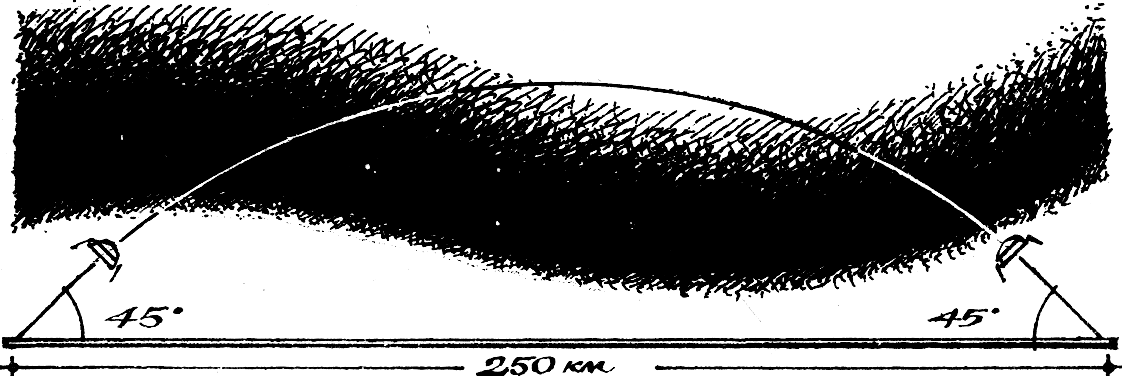
\includegraphics[width=\textwidth]{resume1}

Наиболее трудным заданием первого этапа, как и предполагалось, оказался тренировочный суборбитальный полет на «Лунолете-2» (напомним комплект исходных данных: 1,62 П4 2250 П5 3660 П6 29,43 П7 0 ПА ПВ П0 1 ВП 3 ПД 25 ВП 4 ПС, в регистре 9 — аварийный сигнал). «Я никак не мог с ним справиться,— пишет, например, Н. Плотников из Мончегорска Мурманской области,— Самое большее, сколько я «пролетел», работая с этой программой, это 150 км... Напишите, пожалуйста, как разогнать и на какую высоту поднять «Кон-Тики», чтобы на 1000 кг горючего пролететь 250 км». Н. Плотников не одинок — с этой задачей не справились многие (В. Никифоров из Казани даже решил, что в условиях опечатка — расстояние до цели «равно не 250 км, а 25 км»). Она, кстати, была сформулирована не совсем четко, и некоторые читатели выполняли перелет «в одиночку», с сухой массой корабля 2150 кг (2000+150); такие решения тоже засчитывались. Но решить задачу при 2250 кг, конечно, гораздо сложнее.

«Этот вариант получился у меня не сразу,— честно признается один из победителей первого этапа, В. Алексеев,— недолеты составляли от 50 до 1,5 км. Возникла необходимость экспериментально подбирать время сгорания топлива при разгоне с точностью до 0,1 с. Ход полета: разгон, по возможности вертикальная и горизонтальная скорости должны быть равны, свободный полет, торможение с замедлением, равным ускорению при взлете, начало его приурочено к высоте начала свободного полета». Приводим последовательность команд В. Алексеева (номер маневра: расход /время/ угол, в скобках — показание индикатора) с нашими комментариями. Надеемся, это поможет тем, кто не справился с заданием. Кроме того, она может служить и проверочным тестом к программе «Лунолет-2».

1: 100/3,9/42,5 (149,58601). 2: 100/ 4/42,5	(614,79833).	3:	100/4,1/42,5
(1421,7236). 4: 100/4,3/42,5 (2625,637). 5: 100/4,4/42,5 (4236,0811). 6: 35/1,6/43 (4916,9209). Разгон в основном закончен, реактивное ускорение все время выдерживалось максимально близко к предельному. Угол 42,5\degree выбран, чтобы скомпенсировать действие силы тяжести — вертикальная и горизонтальная скорости сейчас примерно равны; впрочем, практика показывает, что «классический» угол 45\degree ничем не хуже. 7: 2/1/88 (5357,4207). Очевидно, коррекция недолета, получившегося в предыдущей попытке, 8: 0/543,8/0 (4954,3996). После прохождения пассивного участка лунолет оказывается в симметричной точке траектории: расстояние до финиша примерно равно расстоянию от старта в конце разгона, высота приблизительно та же. Теперь начинается интенсивное торможение. 9:	100/4,6/—42 (3138,2379). 10: 100/4,8/—42 (1696,9962). 11: 100/5/—42 (686,8254). 12: 100/5,2/—43 (163,11224). Наиболее ответственный участок пройден. Скорость снижена на порядок, до финиша по прямой осталось примерно 200 м. Можно сбавить темп торможения и выходить к цели. 13: 20/2,2/—44 (75,41972). 14: 20/2,2/—45 (29,758463). 15: 10/2/—42 (15,983541). Лунолет в 16 м над целью, скорость погашена, начинается этап ювелирного прилунения. 16:	5/5/—3	(3,300477).	17:	2/1/1 (1,5622851). 18: 2/1,5/0 (0,7819925). 19: 2/2/0 (0,563843). 20: 1/2/—2 (0). Мастерская посадка! Отклонение практически равно нулю, горизонтальная скорость тоже, вертикальная составила около метра в секунду, а в баках осталось еще полтора килограмма топлива!

В данном случае пилота на финише заботило одно: установить мировой рекорд, прилунившись с точностью менее одного миллиметра (кстати, В. Алексеев после столь же успешно выполненного задания второго этапа был приглашен в КЭИ испытателем поступающих в редакцию игровых программ и в дальнейших полетах участия не принимал — не было времени). В том, что иногда ситуация складывается куда драматичнее, убеждает вариант П. Трубаева из Белгорода (показания индикатора для экономии места не приводятся).

1: 104/4/45. 2: 101/4/45. 3: 97/4/45. 4: 94/4/45. 5: 91/4/45. 6: 48,8/3/45. Как видим, разгон выполнялся под углом 45\degree, а топлива израсходовано даже на килограмм меньше, чем у Алексеева. Посмотрим, каковы будут результаты. 7: 0/520,8/0. Точный выход в симметричную точку. Но чрезмерная точность пилота подвела. Если бы он начал торможение всего на десятую долю секунды раньше, финиш скорее всего происходил бы примерно как в предыдущем варианте. 8: 48/3/—45. 9: 85/4/—45. 10: 82,3/4/—45. 11: 79,6/4/—45. Пилот с завидным хладнокровием повторяет в обратном порядке свои действия при разгоне, но ускорения чуть-чуть отличаются; вот это «чуть-чуть» его и подводит. 12: 77,7/4/—45. 13: 37/2/—45. В последний момент выясняется, что при планировавшейся команде 13: 74/4/ —45, которая по идее должна была вывести корабль на финиш с солидной экономией топлива, лунолет—действительно рядом с финишем — разбивается вдребезги! Не хватает каких-то долей секунды. Поэтому П. Трубаев вдвое уменьшает время маневра, идя на прежнем режиме. В результате ситуация становится критической — до удара меньше секунды; что делать? 14: 24/1,3/0. Естественное решение: пилот над самой целью гасит вертикальную скорость, переходя в горизонтальный полет. И его, конечно же, уносит за точку финиша. Если бы, кстати, он тормознул сейчас не по вертикали, а с , углом -15 или даже -20\degree, все проблемы были бы решены. Но посмотрим за его дальнейшими действиями. 15: 30 /1,7/—80. Вот это да! Большинство, конечно, махнуло бы на все рукой и выполнило посадку метрах в пятидесяти от намеченной точки. Трубаев же подтверждает свою только что заработанную репутацию лихого пилота: истрачено почти все топливо, а лунолет по плавной параболе возвращается к финишу. 16: 0/4/0. 17: 0,6/0,6/30. Последняя капля горючего! 18: 0/1/0. Посадка! Она, правда, получилась слегка жестковатой, но, надо думать, амортизаторы выдержали. Зато не придется топать пешком по серым лунным камням...

Нельзя не остановиться и еще на одном рекордном варианте. А. Аула из Запорожья, выполнивший сначала перелет на корабле массой 2150 кг, узнав, что это не совсем то, решил блеснуть: совершил перелет еще раз, теперь уже при массе 2300 кг! Вот его вариант (только не забудьте изменить содержимое регистра 5: 2300 П5).

1: 4/1/0. 2: 53/2/45. 3: 52/2/45. 4: 51/2/45. 5: 100/4/45. 6: 97/4/45. 7: 94/4/45. 8: 91/4/45. 9: 3/0,2/45. 10: 0/524/0. 11: 87/4/—45. 12: 84/4/ —45.	13: 83/4/—45.	14: 80/4/—45. 15: 77/4/—45. 16: 35/2/—45. 17: 2/1/0. 18: 6,2/0,5/—45. 19: 0,8/0,8/0. Отклонение от цели — меньше полуметра, полная посадочная скорость не превышает 2,4 м/с. Рекорд зарегистрирован и внесен в соответствующую книгу. Если есть желающие побить — милости просим!

«Я купил микрокалькулятор «Электроника БЗ-34» всего три месяца назад, но благодаря КЭИ и подобным рубрикам в других журналах уже умею неплохо пользоваться ПМК,— пишет А.	Сорокин из Кургана.— Все наиболее интересные программы, какие я нахожу в журналах, выписываю в общую тетрадь. Там набралось уже около 40 различных программ, из них почти 20 игровых. Благодаря вашим публикациям я могу теперь использовать ПМК на занятиях. Он стал моим первым помощником. Очень нравится «космический» цикл игровых программ, публикуемый в журнале. Конечно, еще не все получается так, как это нужно для нормального полета. Но с каждым разом я «летаю» все лучше. Хотелось бы, чтобы для разнообразия в журнале появлялись и «земные» программы...»

Подобные пожелания в нашей почте нередки. Стоит сразу определиться: мы публикуем и собираемся публиковать в первую очередь такие игры для ПМК, которые наиболее перспективны в смысле их перевода (с соответствующими дополнениями) на языки персональных компьютеров. К сожалению, абсолютное большинство присылаемых в КЭИ программ реализует несколько общеизвестных игр с простыми выигрышными стратегиями: игра Баше, «Ним» и их разновидности, «Угадай число», «Крестики-нолики», а также простейшие имитационные ситуации типа стрельбы из пушки. Алгоритмы этого рода задач (как правило, далеко не полностью использующих достаточно богатые возможности БЗ-34) довольно подробно рассмотрены в книге Я. Трохименко и Ф. Любича «Микрокалькулятор, ваш ход!» (М., «Радио и связь», 1985). По-настоящему интересные программы почта приносит значительно реже. Наиболее оригинальные из них прислали Д. Кайков из Белгорода, Ю. Пшенник из Харькова, В. Лозовой из Армавира,
B. 	Архипов из Москвы, Г. Горовой из Керчи. Все это вполне «земные» игры, постараемся поместить их в ближайших выпусках КЭИ.

\subsubsection{охота на инопланетных чудовищ}
Начатая в январском номере «охота на инопланетных чудовищ» воодушевила многих читателей на дерзкие вылазки в глубины «электронного океана». Восьмиклассник С. Парамонов из Москвы самостоятельно (еще до выхода февральского номера) сконструировал простейшую «водолазную» программу (возведение в восьмую степень, запись результата в регистр, очистка стека) и поймал Тьму, подавая на вход ЕГГОГи, равные квадратам чисел от 1 ВП 94 до 1 ВП 99. Легко видеть, что его Тьма обитает на глубинах от 1500 до 1600, ровно на 1000 глубже обычной. Если попробовать записать ее в виде единицы с нулями, то она займет почти целый журнальный столбец! Независимо друг от друга В. Соболев из Усть-Каменогорска, С. Козинцев из Кременчуга и C. 	Банников из Москвы очутились в области «длинных монстров» (теперь уже знакомых нам по прошлому выпуску). В. Соболева, учащегося техникума, случайно завела в этот неисследованный район его программа (он работал на МК-61); однако он, в отличие от очевидцев Несси и «Великого морского змея», при встрече с неизвестным животным нисколько не растерялся и, открыв по нему беглый огонь из всех «бортовых орудий», в том числе и «снарядами главного калибра» (отсутствующими на клавиатуре БЗ-34 командами выделения целой и дробной частей), получил интересные результаты в области новых видеосообщений, рассказать о которых придется несколько позже, когда будет обобщен опыт читателей, работавших в данном направлении (МК-61 в распоряжении редакции пока нет). Козинцев же и Банников (оба, кстати, учатся в восьмом классе) прорвались в запретную зону совершенно сознательно, воспользовавшись путем «снизу» (со стороны чисел с отрицательными порядками) и отважно перемахнув «вплавь» (в режиме АВТ) через обширные владения машинного Ноля. Вот как они плыли: 0,01 (количество нулей после запятой может быть произвольным) ВП /—/ 99 Fx$^{2}$. На индикаторе — «длинный монстр» (80,10000000 9), а высказанное в № 1 категорическое утверждение (за пределы Тьмы, дескать, можно проникнуть лишь с помощью специальных программ) полностью опровергнуто!

С.	Банников, кроме того, самостоятельно изучил Тьму (она, по его наблюдениям, представляет собой «нечто вроде джинна, которого надо держать в бутылке»), использовал ее (путем деления на 10200) для вычисления факториалов чисел в интервале от 253 до 293, а главное — открыл способ, который позволяет, не прибегая к помощи коварных чудовищ 4-го этажа, записывать в программу коды, начинающиеся с пустышки. (Это и есть тот «хитрый» прием, что был обещан в № 2.)

Скомандуйте, допустим, В/О КПП8. Калькулятор самопроизвольно переходит в режим ПРГ. Убираем точку — БПРГ. Слева на индикаторе горит 8, справа — 39. Значит, мы, вслед за Сергеем, ухитрились вписать в программу совершенно новую команду (с кодом «пусто — 8»), которой нет ни в одном руководстве по ПМК!

Точно таким же способом Можно «изготовить» остальные команды с кодами «пусто — цифра». Правда, при использовании регистров от 0 до 6 результат зависит от их содержимого; например, если число в регистре 0 заканчивается на 1 или 2, команда В/О КПП0 дает желаемый результат (на адрес 30 вписывается «пусто — 0»; похоже, кстати, на код команды F Вх, но только на первый взгляд — ноль и пустышка поменялись местами), в противном же случае на индикаторе появляется ЗГГОГ-мутант, «расшифровка» которого ни к чему хорошему не приводит. Легко проверить, что любая из этих новых команд в режиме счета по программе выполняет функции «пустой» (в некоторых случаях даже четче, чем КНОП, К1 и К2). Но главное — их коды можно использовать в качестве адресов перехода на последнюю десятку команд длинной побочной ветви 160-шагового цикла, о котором рассказывалось в № 2 за этот год. Других способов добраться до этих мест не существует (кроме довольно-таки утомительной «ходьбы пешком» — ШГ, ШГ в режиме ПРГ; именно так, кстати, совершил «кругосветное путешествие» по всему циклу восьмиклассник Д. Третьякович из Свердловска).

Например, сейчас в программу вписан код «пусто — 8». Если рассматривать его как адрес, то ему соответствует на главной ветви адрес 46. Используем это обстоятельство. F АВТ БП 37 F ПРГ БП (теперь на адресах 37-38 расположилась команда безусловного перехода БП 8) F АВТ БП 46 F ПРГ С/П (эта команда, по идее, должна продублироваться и на адресе «пусто—8») F АВТ БП 37 С/П. После останова переходим в режим ПРГ. Справа горит 9 — мы попали куда хотели. Больше на индикаторе ничего нет — «темная зона».

Еще любопытнее получается, если с помощью, скажем, В/О КППА (или В, С, Д, Е — она же стрелка вверх) F ПРГ вписать в программную память код «пусто — буква» и попытаться использовать его в качестве адреса перехода (ШГ влево ШГ влево БП ШГ влево F АВТ С/П). Куда передастся управление? Для ответа на этот вопрос полезно предварительно расставить на адресах 48-52 подходящие «сети» (вписать туда команды С/П), а после останова перейти в режим ПРГ. Редакция честно предупреждает: результат будет весьма неожиданным.

Михаил ПУХОВ

\section{ПРОГУЛКА ПО «ЛУНОЛЕТУ»}
\begin{figure}[H]
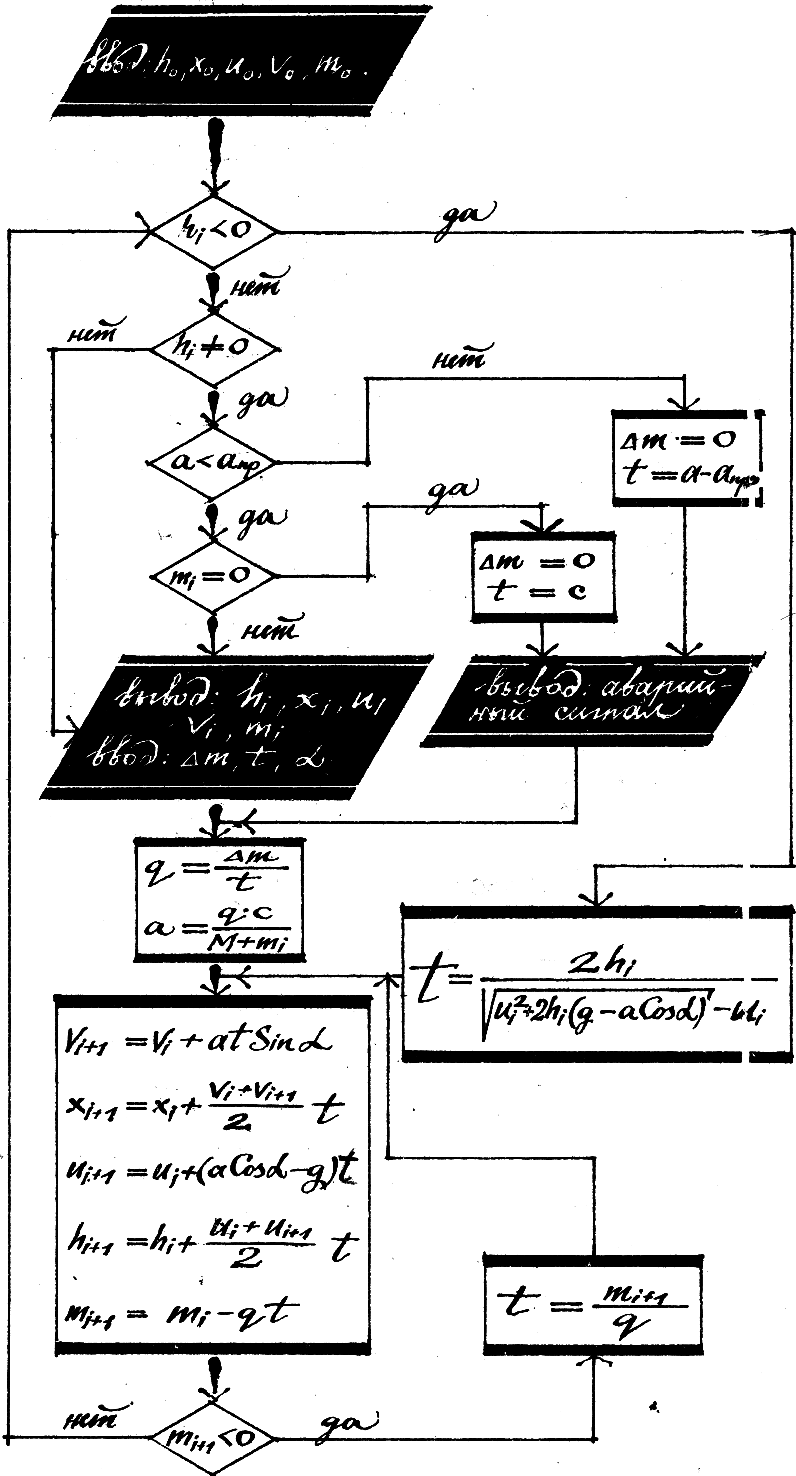
\includegraphics[width=0.5\textwidth]{lunolet2_algo}
\caption{Блок-схема программы "Лунолёт-2"}
\end{figure}

Вряд ли кто из читателей «ТМ» переходит улицу с закрытыми глазами. Обычно мы придерживаемся строго определенного правила — подойдя к краю тротуара, останавливаемся, смотрим влево, оцениваем обстановку, доходим до середины улицы, затем смотрим вправо и либо пропускаем транспорт, либо заканчиваем переход. Как скажет математик, мы действуем по вполне определенному алгоритму.

Сегодня это слово можно услышать в разговоре людей самых различных профессий. Но термин «алгоритм» вовсе не порождение XX века. Это просто трансформированное имя средневекового математика аль-Хорезми (в переводе — «из Хорезма»). Его книга об искусстве вычислений в десятичной позиционной системе счисления во многом способствовала распространению в Европе столь привычных нам цифр и методов счета. В средние века европейцы называли алгоритмом именно десятичную систему и правила арифметических действий в ней. Все математики того времени даже делились на две группы — абацистов, которые вели расчеты на абаке, и алгоритмиков, владевших приемами письменных вычислений.

С тех пор смысл слова «алгоритм» изменился. Сегодня мы так называем набор правил для решения той или иной задачи. Сформулировать их можно поразному.

Очень удобно представление алгоритмов в виде блок-схем, на которых хорошо видны структура алгоритма и связи между его отдельными частями. Подобно тому, как географическая карта позволяет туристам и путешественникам ориентироваться на местности, так и блок-схема помогает программисту «прокладывать маршрут».

С этого номера Клуб электронных игр (КЭИ) начал печатать «карты для программистов», то есть блок-схемы. Давайте же воспользуемся одной из них и совершим «путешествие» по алгоритму программы «Лунолет-2». Надеемся, что оно облегчит нашим читателям работу над собственными программами.

Итак, обратимся к рисунку. В его верхней части мы видим блок ввода исходных данных — вертикальной и горизонтальной скоростей, запаса топлива и координат точки старта. Затем следует несколько проверочных блоков. Об их назначении и работе мы поговорим несколько позже, а сейчас перейдем к блокам вычисления текущих значений вспомогательных и основных переменных.

Прежде всего несколько слов о физической стороне задачи. На ракету, находящуюся в постоянном гравитационном поле при отсутствии атмосферы (а именно такая простейшая модель использована в программах «Лунолет-1» и «Лунолет-2»), действуют сила тяжести и тяга двигателя. Величина реактивного ускорения зависит от секундного расхода топлива, а направление определяется углом тяги. Этот угол вводится непосредственно (см. темный блок в середине рисунка). Кроме того, здесь же вводятся расход топлива на данном шаге и время, за которое он производится. После этого блок вычисления вспомогательных переменных определяет секундный расход и реактивное ускорение. Эти результаты передаются в блок вычисления текущих значений основных переменных.

Его задача — найти значения координат и скоростей после отработки двигателя. Так как ускорения постоянны, то используются хорошо знакомые из школьной физики формулы равноускоренного движения. Одновременно подсчитывается и количество оставшегося топлива.

Теперь, казалось бы, самое время выводить полученные величины на индикатор, но на рисунке путь к блоку вывода почему-то извилист и лежит через несколько проверок. В чем дело?

Действительно, игровые программы принципиально отличаются от обычных расчетных. Когда мы просто решаем уравнения, то действуем по принципу «куда прилетели, туда и прилетели». Вычислительная техника, неважно, компьютер или микрокалькулятор, подсчитывает координаты и скорости в конечной точке и выводит их на дисплей или индикатор. Нам остается только ознакомиться с результатами. В игровой же программе мы периодически вводим управляющее воздействие, в нашем случае — изменяем величину и направление реактивного ускорения. Но ведь это можно сделать не всегда. Если, скажем, ваш лунолет превратился в «землерой», то есть высота получилась отрицательной, дальнейшая игра бессмысленна. Чтобы выявить такого рода ситуации, в алгоритм и введены блоки проверок. Посмотрим же, как они работают.

Прежде всего выясним, сколько топлива осталось после маневра? Если запас окажется меньше нуля, значит, такой маневр невозможен, ведь летать на «отрицательном топливе» нельзя. Нужно вернуть лунолет в ту точку траектории, где кончилось горючее. Микрокалькулятор определяет, сколько секунд назад опустели баки, и передает это значение (отрицательное!) в блок вычисления основных переменных. Там оно подставляется в уравнения движения, и «бортовой компьютер» отводит наш летательный аппарат назад, по той же самой траектории, в точку, где иссякло топливо. Именно с ее координатами и соответствующими скоростями продолжает работать программа.

Следующей «становится на проверку» высота. Если она неотрицательна (выход из блока сравнения по стрелке «нет»), то все в порядке. Если же лунолет уже «забурился» в недра планеты, надо извлечь его оттуда. Как это сделать;?

«Бортовой компьютер» исправляет ошибку пилота тем же методом, что и в случае перерасхода топлива. Подсчитывается время «полета» под поверхностью планеты, и его значение (опять- таки отрицательное) передается в блок вычисления основных переменных. Лунолет возвращается по траектории назад, в точку финиша. Блок вывода сообщает о том, где мы оказались (значение горизонтальной координаты) и насколько мягкой была посадка (величины скоростей). Если же высота еще положительна, то наступает черед следующей проверки — «биологической».

Из-за слишком большой перегрузки экипаж лунолета мог потерять сознание (выход по стрелке «нет»). В этом случае управление берет на себя автоматика — выводится аварийный сигнал, останавливается двигатель, и некоторое время полет происходит по инерции. Оно определяется разностью реактивного и предельно допустимого для пилотов ускорений, что достаточно разумно для игровых программ. Блоки вычисления переменных определяют, где окажется аппарат, когда экипаж вновь сможет «взять в руки штурвал». Если же перегрузки не превысили нормы, то мы выходим из блока сравнения по стрелке «да» на последнюю проверку: наличия топлива.

При пустых баках управление вновь передается бортовому компьютеру — он задает нулевой расход (ведь летать- то уже не на чем), большое .(порядка тысяч секунд) время и передает эти данные в блок вычислений. Пилотам остается лишь. созерцать аварийный сигнал и ждать, когда они «куда-нибудь свалятся» (по меткому выражению Лунного Коршуна). Если же топливо еще есть, то можно продолжать полет. ПМК «докладывает обстановку» и ждет очередной команды с пульта.

Приведенная блок-схема удобна для постановки игры на персональном компьютере, так как его возможности несравненно больше, чем у микрокалькулятора.

Первые шаги в этом направлении уже сделаны. «В соответствии с Основными направлениями реформы общеобразовательной школы исполнительный комитет Октябрьского районного Совета народных депутатов Тюменской области определил меры по обеспечению компьютерной грамотности учащихся средних школ района,— пишет в редакцию председатель исполкома А. М. Вахонин.— Постановлением Октябрьского районного комитета КПСС и Октябрьского райисполкома от 24 апреля 1985 года принято решение создать вычислительный центр в опорной Сергинской средней школе и серьезно оснастить его новейшими современными персональными компьютерами, выделив на это материальные средства от базовых предприятий, и считать этот центр учебно-методической базой в масштабе школ района по изучению методики преподавания основ информатики и вычислительной техники... В настоящее время создана лаборатория, где установлены две микро-ЭВМ ДЗ-28, дисплеи ИЭ-00-13, термопечатающее устройство... Машины работают по 9 часов в сутки, машинного времени, чтобы удовлетворить всех желающих, явно не хватает — мало машин. Интерес к вычислительной технике и программированию чрезвычайно высок.

Особенно заинтересовались дети статьями о фантастических электронных играх на космические темы, напечатанными в журнале «Техника — молодежи». Девятиклассники Латыпов Урал и Заволока Владимир, слушатели факультатива «Программирование на БЕЙСИКе», решили перенести все эти игры на машину ДЗ-28. Сейчас программа «Лунолет-1» переведена на язык БЕЙСИК. Программисты полностью разобрались в алгоритме, нарисовали блок-схемы. Программа получилась очень красивой, с интересными комментариями, объяснениями непонятных ситуаций, возникающих при взлете и посадке. Игра идет в виде урока, который ведет ЭВМ. Сейчас началась работа над «Лунолетом-2». В перспективе — все ваши интереснейшие программы перенести на микро-ЭВМ».

Мы ознакомились с программой тюменских школьников, любезно предоставленной руководителем юных программистов С. П. Митрофановым. Сделана она достаточно профессионально, кроме того, ребятам не откажешь в чувстве юмора. Так, при посадке со скоростью, превышающей 10 м/с, на дисплее появляется сообщение: «Я вас могу успокоить лишь тем, что по вас плачут родственники и друзья». Если же посадка была удачной, то компьютер «присваивает вам очередное звание» (вплоть до генерала) и предлагает совершить следующий полет в более сложных условиях. Кроме того, игра снабжена и комплексом предстартовых проверок, когда надо ответить на ряд несложных теоретических вопросов, касающихся будущего полета. Но здесь надо быть осторожным и внимательным. По крайней мере, представитель администрации КЭИ, заявивший, что выдерживает пятнадцатикратные перегрузки, немедленно был «снят с полета за хвастовство».

Персональный компьютер позволяет также вести игру в реальном масштабе времени. Это, конечно, приближает ее к действительности. Пока администрация КЭИ такими программами не располагает и надеется здесь на помощь читателей.

Сергей АЛЕКСЕЕВ, инженер

\section{сделай сам СЕБЕ РАКЕТУ}
Как видим, наше клубное помещение постепенно обставляется новой мебелью (блок-схемами), виртуозно сработанной художником Евгением Катышевым. Из-за этой замечательной мебели (блок-схем) оно все больше теряет привычные контуры детской площадки для игр, становясь похожим скорее на научную лабораторию или в крайнем случае на машинное отделение (отсек, в котором стоят ЭВМ) какого-нибудь фантастического фотонно-подпространственного звездолета...

Впрочем, надо признать со всей откровенностью: для многих читателей нашей рубрики всякие игры кончились уже после выхода «ТМ» № 9 за прошлый год. Космонавтика, как выяснилось, не игра, а работа, и работа довольнотаки утомительная. «При орбитальных переходах... слишком долго ждать результата. Виток, два витка, иногда больше. Причем каждый виток — это полтора часа, два... Вот и крутишься. Изматывает...» — так характеризовал ситуацию М. Коршунов. Можно, конечно, махнуть рукой на цели и задачи «Кон-Тики» и просто играть. Так, О. Роженцов из города Голицына Московской области взял большой лист миллиметровки, начертил замысловатый лабиринт, ввел в ПМК программу «Лунолет-2» и... Вот что он рассказывает: «Изменяется просто смысл игры. Теперь она заключается в прохождении корабля по лабиринту. Цель может быть разной (например, сесть в то же место, если трасса замкнута). Исходные данные лучше изменить: ускорение свободного падения задать равным нулю, уменьшить скорость истечения продуктов сгорания, разместить в лабиринте промежуточные заправочные станции и т. д. Эту игру можно использовать и для двух игроков с двумя ПМК, например устроить гонки на трассе...»

А вот еще один небезынтересный опыт. «Получил массу удовольствия, гоняя на «Кон-Тики» по всей Луне,— пишет А. Арсеньев из города Березники Пермской области.— Получил немало «шишек», много моих «могил», увенчанных обломками «Кон-Тики», осталось на поверхности нашего естественного спутника. Методом «тыка и вытыка», как у нас говорят, освоил выход на орбиту и сход с нее. К сожалению, дефицит свободного времени не позволил мне принять участие в перелете на Землю. Поэтому, начиная со стыковки со станцией «Юрий Гагарин», я стал наблюдателем и болельщиком. Уже в окололунном орбитальном полете начинает ощущаться недостаточный динамизм обстановки. Виной тому — малый шаг приращения времени и фактическое бессилие оператора, «болтающегося» на орбите. Именно из-за этого я увлекся «высшим пилотажем»: не выключая двигателя, меняя лишь направление вектора тяги, делал мертвую петлю в горизонтальном полете на небольшой высоте...»

Тем не менее, несмотря на все объективные и субъективные трудности (присутствующие, кстати, и в реальном полете), большая группа читателей не только аккуратно выполняла предлагавшиеся задания, но и ежемесячно представляла в редакцию (ЦУП — «ТМ», как метко окрестил КЭИ А. Морев из Устинова) объемистые отчеты о каждом этапе полета. Основным «транспортным средством» для тренировочных орбитальных полетов служили программы «Лунолет-3» и «Вершина». Их обобщенная блок-схема приведена на рисунке, ее подробное описание можно найти в разделе «Алгоритмическая гимнастика». Дополнительно к программе «Лунолет-2» введены следующие постоянные и переменные величины: К — гравитационная постоянная планеты, равная произведению квадрата ее радиуса на ускорение свободного падения на поверхности; R — радиус планеты; r — текущее расстояние от ее центра; $\phi$ — угловая координата; V$_{kr}$ — круговая скорость на данной высоте. Рельеф учитывается заданием какой-либо зависимости радиуса планеты от угловой координаты.

Программы «Лунолет-3» и «Вершина» реализуют упрощенные варианты приведенной блок-схемы. В первой из них счетный блок сохранен полностью, зато использован упрощенный посадочный блок, подробно описанный в «ТМ» № 3-4 за этот год. Радиус планеты считается постоянным. Конкурсное задание по «кругосветному» путешествию особых затруднений не вызвало (разумеется, у тех читателей, кто благополучно сплавился с баллистическим перелетом на 250 км). Что же касается «скрытых» возможностей ПМК (а участники перелета, и это радует, проявили себя не только мужественными пилотами, но и высококвалифицированными бортинженерами: смело вносили изменения в опубликованные программы и разрабатывали свои собственные), надо отметить предложение десятиклассника Льва Роканиди из Сызрани: хотя он несколько задержался с представлением отчета, зато придумал оригинальный способ преобразования сообщения (Е—0) в (Е 0—) с помощью команды ВП 9 КНОП. Этот способ, по убеждению администрации, открывает пути дальнейшего совершенствования данной серии космических аппаратов.

«Кон-Тики» выходил на орбиту поразному, но на это всегда уходило несколько больше двух тонн топлива (вспомним: «Ракете легче финишировать, чем стартовать, потому что на финише она сама легче»). Приведем, например, мнение А. Артамонова из города Апрелевки Московской области. «Режим вывода аппарата на орбиту таков. Сначала его нужно разогнать на малой высоте до первой космической скорости. При этом израсходуется большая часть топлива и аппарат станет легче примерно на 2 т. Затем (достигнув нужной высоты.— М. П.) придать ему дополнительный корректирующий импульс и вывести на круговую орбиту. Как указано в тексте, никаких особых препятствий, кроме горного хребта на обратной стороне Луны, на пути аппарата нет. Поэтому разгон на малой высоте, по-видимому, можно считать допустимым».

Надо сказать, что участники тренировочных рейсов в ряде случаев оценивали свои действия без намека на зазнайство и хвастовство, с ощутимым элементом самокритичности. «Несколько дней и ночей, отрываясь нехотя лишь на еду и кратковременный сон, я методично разбивал лунолет за лунолетом, «размазывая» их по поверхности»,— пишет студент ЛГУ Д. Журавлев, делясь своим первым опытом пилотирования ракетных аппаратов. «Посадка без больших повреждений,— рапортует А. Морев.— Недолет, правда, порядка 1500 м. Но, вероятно, посадочная площадка космодрома позволит мне несколько удалиться от ее центра». И так далее.

В программе «Вершина» гравитационное, кориолисово и центробежное ускорения не зависят от высоты, зато имеется рельеф: отклонение радиуса планеты от нулевой отметки в окрестностях начала координат задается колоколообразной кривой, носящей красивое математическое название «локон Аньези». Кроме того, в «Вершине» использован тот же посадочный блок, что и на нашей блок-схеме. Все тот же неутомимый в своих критических замечаниях Л. Роканиди и С. Вардин из Москвы выражают (в письменной форме!) свои сомнения по поводу рекомендуемой для программ «Вершина» и «Маскон» формулы для расчета круговой скорости; по их мнению, команду ИП7 следует заменить на ИПА, ибо, по словам С. Вардина, «из текста следует, что от высоты не зависит ускорение силы тяжести, а не круговая скорость (что было бы странно!)».

Необходимо дать пояснение. Как уже отмечалось, сила тяжести в этих программах считается постоянной. Естественно, это верно лишь в узком приповерхностном слое. Поэтому круговая скорость в программе «Вершина» действительно не зависит от высоты; если согласиться с поступившими предложениями, она, вместо того чтобы уменьшаться с высотой, увеличивалась бы (что было бы действительно странно!). Впрочем, при полетах на малых высотах это особого значения не имеет.

М. Точин из Вологды, Ю. Кузнецов из Куйбышева и А. Аула из Запорожья сообщили, что в программе «Вершина», по их мнению, содержится ошибка: происходит ее зацикливание, причем команда с пульта С/П В/О С/П не помогает — программа снова зацикливается. Естественно, критика предлагается конструктивная — все трое изобрели различные методы устранения неприятности, основанные на модернизации алгоритма посадки. Однако главное достоинство посадочного блока программы «Вершина» — возможность выполнения посадки на крутом склоне, причем даже в горизонтальном полете, — при этом теряется.

Разбор показал:
\begin{enumerate}
\item После ввода исходных данных, опубликованных в журнале, лунолет в начальной позиции находится, как правильно подметил М. Точин, на высоте —6,2 м, то есть как бы в стартовом колодце. Причина в том, что подошва горы, перелет на которую надлежит выполнить, тянется довольно далеко. Если стартового импульса не хватает, чтобы вывести корабль из колодца, программа действительно зацикливается (это легко проследить по блок-схеме). Если же импульс достаточен, никакого зацикливания не происходит и можно смело лететь дальше.
\item Из-за медленной сходимости метода половинного деления и малого быстродействия ПМК при посадке корабля может сложиться впечатление, что программа зацикливается. У пилота возникает искушение остановить программу с пульта (С/П), скомандовать В/О С/П и продолжить вычисления. Такие действия приводят к неправильному выходу из подпрограммы, стековая память адресов возврата засоряется, и происходит зацикливание. Подобная неприятность может случиться и в других программах, использующих вложенные друг в друга (наподобие матрешек) подпрограммы.
\item Избавиться от зацикливания в подпрограмме можно следующим образом: отдать с пульта команду С/П, а затем повторить несколько раз последовательность БП 92 ПП, пока не произойдет передача управления на адрес 01. После этого командой В/О С/П можно вновь запускать программу (вместо адреса 92 можно использовать любой другой, на котором записана команда В/О — в нашем случае 85).
\end{enumerate}

Надо отметить, что не все читатели вели свои корабли к вершине по низкой окололунной орбите. Некоторые, «тряхнув стариной» (вспомнив предыдущее задание), совершили баллистический суборбитальный перелет, сэкономив на этом деле без малого две тонны топлива. Поскольку в задании ничего не говорилось о выходе на орбиту, это совершенно правильное решение.

О программе «Маскон» поговорим особо. Вероятно, целесообразно обсудить ее вместе с «Лунолетом-4». («Луна — это маскон! Маскон — концентрат массы в гравитационном поле планеты!.. Увеличь Землю до размеров лунной орбиты, тогда ты меня поймешь!»)

На «устные» задания тура удачнее всех, по нашему мнению, ответил восьмиклассник В. Ладохин из города Сургута Тюменской области, задержавшийся, кстати, на старте суборбитальных полетов: «Прошу меня извинить за то, что опоздал, просто калькулятор мне купили недавно». В ЦУП—«ТМ» причина признана уважительной. Начиная с задания № 2 В. Ладохин стал одним из наиболее дисциплинированных участников перелета.

Напомним заданные вопросы:
\begin{enumerate}
\item 4) 	Прав ли был Коршунов, когда демонтировал 50 кг навигационной аппаратуры? Зачем он так поступил?
\item 5) 	К какому приблизительно перерасходу топлива привела встреча «Кон-Тики» с масконом?
\item 6) 	Видите ли вы какой-нибудь выход из сложившейся на «Кон-Тики» ситуации (кроме того, который предлагает Коршунов)?
\end{enumerate}

А вот ответы Вадима:
\begin{enumerate}
\item 4) 	Коршунов был прав. Так как лунолеты типа «Кон-Тики» не предназначены для орбитальных полетов, то и аппаратура у них была соответствующая. Поэтому при орбитальном, а тем более межпланетном полете большинство приборов «Кон-Тики» будет бесполезным грузом.
\item 5) 	При встрече «Кон-Тики» с масконом перерасход топлива составил не более 5 кг.
\item 6) 	Я думаю, что идти за борт никому не надо. Топлива на посадку хватит.
\end{enumerate}

* * *

«По завершении рейса «Кон-Тики» хотелось бы увидеть в этом разделе новые игровые программы,— пишет девятиклассник Е. Бедекер (ст. Полетаев Челябинской области).— С их помощью, кроме удовольствия, полнее узнаешь возможности своего ПМК. Но вот еще было бы объяснение принципа составления и нюансов этих программ. Чтобы программа виделась осмысленным рядом действий, а не бездумным набором знаков. Чтобы с помощью вашего журнала научиться не только исполнять готовые программы, но и составлять их самому».

«С помощью МК-54 и программ, публикуемых в журнале, мы с другом совершили несколько увлекательных путешествий,— развивает похожую точку зрения 17-летний А. Дибривный из Херсона.— Нам бы хотелось совершить более сложные путешествия — к комете Галлея, к другим планетам Солнечной системы, к другим звездам, но мы не знаем, как составить программы для таких путешествий. Не могли бы вы рассказать, как можно составить такие программы, помочь нам в их составлении?»

«Я не думал о ПМК, но благодаря вашим публикациям попросил на день рождения именно программируемый,— сообщает не назвавший своего возраста Д. Евдокимов из Ленинграда.— В конце октября мне купили с трудом (дефицит почему-то!) МК-54. Теперь я осваиваю ваши программы. Спасибо вам за них! То, что вы придумали этот клуб, очень здорово! Но посвятите хотя бы один номер тому, как самому придумывать игры. Составить программу решения уравнения легко, а игру никак... Научите составлять игры!»

Что ж, пожелания законные, давайте придумаем игру вместе. По глубокому убеждению администрации, главное — это название. Назовем ее, скажем, «Многоступенчатая ракета». Ясно же, что на лунолете класса «Кон-Тики» далеко не улетишь, даже взлететь с Земли вряд ли удастся. Поставим задачу так: количество ступеней произвольно, после команды на отделение ступени задействуется следующая. Желательно, чтобы программа в обращении не была сложнее «Лунолета-3», который и возьмем за основу. Неплохо было бы сохранить и видеосообщения. Договоримся все постоянные и переменные величины оставить в прежних регистрах. Только теперь в регистре Д разместится запас топлива первой ступени, а в регистре 5, ясное дело,— ее «сухая» масса плюс полная масса всех последующих ступеней, включая полезную нагрузку.

Посмотрим, какие внутренние резервы есть у нашего «Лунолета-3». Команды, записанные по адресам 12-18, никакой роли не играют, просто повышают сервисность программы, рассчитывая и переводя в регистр Y круговую скорость на данной высоте. Это семь команд. Можно ли уместить сюда «многоступенчатый блок»?

Возьмем простейший случай. Пусть при зажигании двигателя каждой ступени полная масса ракеты распределяется поровну между следующими компонентами: 1) масса топлива нижней ступени; 2) масса ее конструкции; 3) масса всех последующих ступеней, включая полезную нагрузку. Легко видеть, что после команды на отделение ступени необходимо проделать следующие операции:

\begin{enumerate}
\item разделить оставшуюся массу ракеты (содержимое регистра 5) на 3;
\item полученное число записать в регистры 5 и Д;
\item вернуться на начало программы.
\end{enumerate}

Наиболее простая последовательность команд, реализующая данный алгоритм, такова (адреса условные): 01.ИП5 02.3 03.$\div$ 04.П5 05.ПД 06.БП 07.00. Уложились ровно в семь команд! Блок сконструирован, но куда его вставить? И каким образом, не усложняя работы с программой, отдавать команду на разделение ступеней???

Обратим внимание на блок-схему, на то место, где производится проверка на перерасход топлива. Если вы внимательно следите за «топливными ресурсами», она бесполезна. Что, если команду с перерасходом сделать сигналом на отделение ступени? Значит, надо сделать так, чтобы при перерасходе управление перешло на только что сконструированный «блок многоступенчатости»!

Тот, кто хочет внести необходимые исправления сам, может «приглушить звук». Для остальных сообщаем алгоритм преобразования «Лунолета-3» в «Многоступенчатую ракету»:

\begin{enumerate}
\item Выбросить из программы команды по адресам 12-18;
\item Команды по адресам 19-26 «сдвинуть» вверх. Теперь они будут занимать адреса 12-19.
\item Вписать на адреса 20-21 команды 20. Fx<0 21. 29.
\item Вписать на адреса 22-28 только что сконструированный «блок многоступенчатости».
\end{enumerate}

Ракета построена. Вводите видеосообщения, нужные вам исходные данные, заливайте в баки горючее, определите себе цели полета — и в путь! Только администрация настоятельно рекомендует: внимательно следите за содержимым регистра 5. Ведь это масса всех пока еще бездействующих ступеней, включая полезную нагрузку. Не забывайте, что в нее входите и вы сами! И если команда ИП5 на очередном останове выдаст на индикатор, скажем, число 100, администрация обоснованно опасается, что вам, увы, уже ничто не поможет...

«Недавно просматривал ваш журнал № 10 за 1985 год, в частности рубрику «Клуб электронных игр», и возникло желание спросить: почему сообщение микрокалькуляторов типа БЗ-34 и МК-54 по ошибке ERROR на страницах вашего (впрочем, не только вашего) журнала печатается в виде ЕГГОГ? — справедливо недоумевает А. Федоренко из Новосибирска.— Если это результат стремления избежать дополнительных трудностей при наборе, то оправдано ли такое стремление, в результате которого вместо осмысленного и понятного (по крайней мере, переводимого) слова появляется какой-то птичий набор?»

Отвечаем по существу. Для нас и наших читателей ЕГГОГ в первую очередь это: 1) условное обозначение чисел с порядками между 100 и 200 (см. № 1 с. г.), которые можно, например, записывать в регистры, отдавать по ним команды косвенной адресации (об этом еще расскажем) и т. д.; 2) своеобразное «прикрытие», пользуясь которым можно вызывать в регистр X и подвергать различным операциям числа, которые иначе вызвать не удается, скажем Тьму (№ 3); 3) универсальное «сырье», из которого можно получать такие полезные продукты, как символы Е, Г, С, L и —. Даже язык как-то не поворачивается назвать столь бесценное сокровище «ошибкой», пусть даже на английском языке...

Кстати, насчет символов Е, Г и т. д. «Почему вы написали, что после адреса 99 идут (в БЗ-34) адреса А0...А9, В0...В9,	С0...С9,	Д0...Д9,	Е0...Е9, 0...9? — просит разъяснений заинтересовавшийся проблемой 160-шагового цикла А. Коротков из Тулы — У меня они идут в следующем порядке: —0...—9,	L0...L9, С0...С9,	Г0...Г9, Е0...Е9, 0...9. А «темная зона» начинается с адреса СЗ, а не С1, как сказано у вас».

Охотно даем разъяснения. Во-первых, символы —, L и Г есть соответственно коды букв А, В и Д, так что никакого противоречия в первом обнаруженном факте нет. Кстати, странички нашего клуба (или стены?) пронумерованы именно этими кодами. Второе замечание справедливо — «темная зона» начинается не с адреса С1 (что было бы странно!), а с адреса С0. При переходе же на адрес С2 она сплошь заполняет индикатор.

Наконец, сообщение, которое, несомненно, порадует всех любителей, если можно так выразиться, «компьютерной грамматики». Буквально накануне отправки номера в производство администрация КЭИ получила сенсационную телефонограмму следующего содержания:

«Извещаю, что мною получен простой способ формирования на БЗ-34 любых комбинаций из цифр и символов Е, Г, С, L, —, не начинающихся с 0. Для этого нужно ввести в ПМК следующую программу: 00.КИП0 01.ВП 02.7 03.П9 04.КИП9 05.КИП$\uparrow$ 06.ИП9 07.\XY 08.\XY 09.ВП 10.ВП 11.1 12./—/ 13.FL0 14.03 15.С/П.

После ввода программы нужно сформировать и ввести в регистры 1, 2 и т. д. вплоть до 8 необходимые символы в том же порядке, в каком они входят в состав необходимого слова. Например, если вы хотите получить на индикаторе «слово» ГО-ГО-ГО, нужно ввести букву Г в регистры 1, 4 и 7, обнулить регистры 2, 5 и 8, ввести символ «—» в регистры 3 и 6. В регистр 0 заносится число букв в слове, не считая замыкающих его нулей, плюс один. В нашем случае 8. Теперь В/О С/П. Через десяток секунд на индикаторе появляется заказанное вами слово (с точностью до положения десятичной точки, но она легко переносится с помощью команды ВП).

Сообщаю также, что мною сконструирован инструмент для программного получения символов Е, Г, С, L и —. Вот соответствующая программа: 00.$\uparrow$ 01.Cx 02.\XY 03.\XY 04.ВП 05.С/П. (По адресу 00 вписана стрелка вверх.) Если подать на ее вход цифру 9, после останова получим —. Если —, то L. Букву Е лучше не вводить — она дает «пустышку», а это символ весьма опасный.

В. Архипов».

Администрация КЭИ объявляет Владимиру Архипову благодарность и в этой связи дает следующее задание:
\begin{enumerate}
\item Получить максимальное число осмысленных слов и прислать их.
\item Придумать, каким образом, несмотря на Категорическое утверждение нашего постоянного корреспондента, можно зафиксировать на индикаторе и записать в адресуемые регистры, скажем, названия программ «ОС-1», «ОС-2», «ОС-3».
\end{enumerate}

Михаил ПУХОВ

\section{ПРОГРАММА С ПРИПЕВОМ}
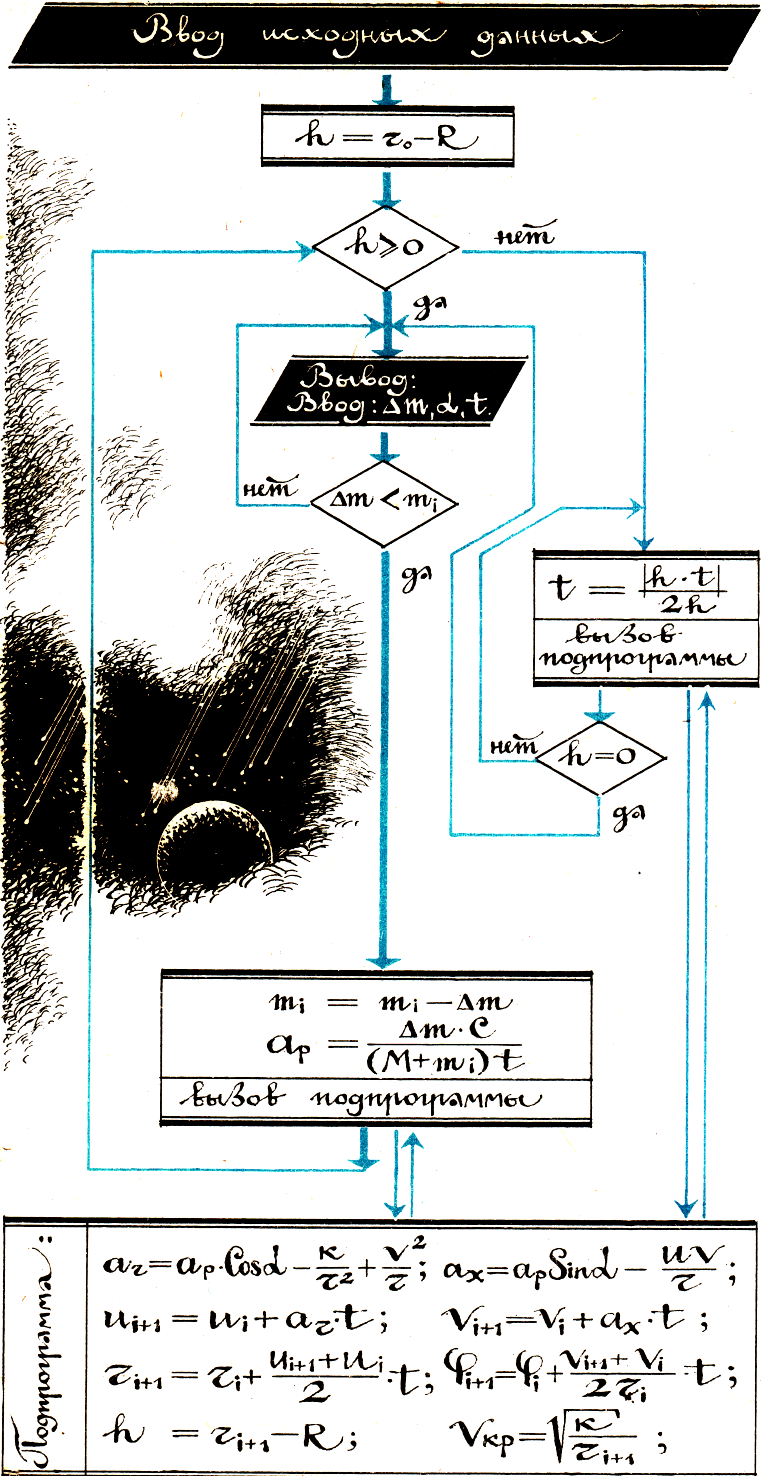
\includegraphics[width=0.5\textwidth]{subprg}

Как печатают текст какой-нибудь песни? Сначала первый куплет, потом припев, потом второй куплет, а потом... лишь одно слово — «припев». Точно так же и после третьего куплета, если он, конечно, есть и т. д. В самом деле, зачем несколько раз печатать одни и те же строчки, когда достаточно указать, лишь где их нужно исполнять.

Аналогичная ситуация встречается и в программировании. Например, решая системы дифференциальных уравнений, приходится неоднократно вычислять правые части уравнений, при этом алгебраические формулы одни и те же, изменяются лишь значения входящих в них переменных. Конечно, нецелесообразно в такой задаче многократно выписывать в программе одно и то же. Специалисты давно придумали способ составления программ с «припевом». Повторяющаяся часть программы записывается только один раз в виде отдельного блока, которому присваивают собственное имя (набор цифровых или буквенных символов), чтобы его можно было отличить от других. Такие блоки носят название подпрограмм. Теперь, когда требуется обратиться к подпрограмме, то в тексте основной программы ставится специальный оператор вызова подпрограммы, вслед за которым указывается ее имя.

После того как мы познакомились с понятием подпрограммы, пора открыть небольшой «секрет» — возможно, что многие члены КЭИ оказались в положении мольеровского Журдена, который говорил прозой, не зная, что он говорит прозой. Ведь мы уже давным-давно использовали подпрограммы, путешествуя на «Кон-тики» вместе с Лунным Коршуном. Чтобы убедиться в этом, обратимся к блок-схеме «орбитальной» программы. Прежде всего о физической стороне задачи. Мы рассматриваем полет ракетного летательного аппарата по орбите вокруг безатмосферной планеты. При этом, кроме тяги двигателя и притяжения небесного тела, на лунолет действуют центробежная и кориолисова силы, дающие вклад в вертикальное и горизонтальное ускорения соответственно.

Ну а теперь пора «запевать песню», то есть проследить по блок-схеме работу программы. Сначала вводятся исходные данные, необходимые для совершения полета,— характеристики планеты и аппарата, начальные значения переменных. Затем вычислительная система определяет начальную высоту, так как в уравнениях движения в качестве текущей переменной выбрано расстояние от центра планеты. Далее идет уже знакомый нашим читателям по предыдущему выпуску рубрики блок проверки положительности высоты. Основную роль он играет при дальнейших маневрах, а сейчас мы просто выходим из ромба по стрелке «да» — ведь не искать же полезные ископаемые в недрах планеты мы собрались? И наконец, беремся за рычаги управления — вводим значения расхода топлива, угла тяги и время маневра.

Но прежде чем начать полет, бортовой компьютер проверит, не перерасходуем ли мы топливо. Если все в порядке — выход из блока проверки по стрелке «да», то приступает к работе блок вычисления реактивного ускорения. Он действует аналогично такому же блоку в программе «Лунолет-2» (см. «ТМ» № 5 за 1986 год). Кроме ускорения, этот же блок подсчитывает и запас оставшегося топлива. Итак, «куплет пропет», переходим к «припеву»,—обращаемся к подпрограмме, которая определяет значения текущих переменных.

Несколько слов о ее работе. В первую очередь вычисляются составляющие ускорения — вертикальная и горизонтальная. Первая определяется проекцией реактивного ускорения на вертикаль, гравитационным ускорением, которое в нашем случае может быть переменным (так как меняется радиус орбиты), и центробежным ускорением. Вторая — проекцией реактивного ускорения на горизонтальное направление и кориолисовым ускорением. При нахождении проекций скорости и значений текущих координат используются обычные формулы равноускоренного движения, которые при своей простоте обеспечивают достаточную точность для задач подобного типа.

После окончания «припева» мы возвращаемся в основную программе и снова проверяем положительность высоты. Если полет проходит в нормальных условиях (выход из блока проверки по стрелке «да»), то опять беремся за рычаги управления и еще раз повторяем «куплет — припев». Наша «песня» продолжается до тех пор, пока мы либо благополучно не завершим перелет, либо...

«Этот человек... Бёрст врезался в Луну»,— писал Станислав Лем в одном из рассказов о пилоте Пирксе. Ну что ж, никто не гарантирован от неудачи, и в нашем полете возможна ситуация, когда неосторожный маневр приводит к тому, что лунолет оказывается погребенным в недрах планеты (из блока проверки высоты мы выходим по стрелке «нет»). Нужно извлечь его оттуда. Это мы уже делали в программе «Лунолет-2», но сейчас предлагаем вам еще один метод. Как и в предыдущем случае, «спасение утопающих» оказывается делом не их рук, а микрокалькулятора. Время неудачного маневра делится пополам, причем знак его оказывается совпадающим со знаком высоты — если высота отрицательна, то и время отрицательно. Потом происходит обращение к подпрограмме, в нее вводится полученное отрицательное время, и лунолет проводится по траектории назад, при этом находится новое значение высоты. Затем оно сравнивается с нулем. Если высота занулилась, а при ее вычислении заодно происходит ее округление, программа заканчивает свою работу, прилунение (удачное либо неудачное) завершено. Если же высота отлична от нуля, то бортовой компьютер продолжает трудиться: время вновь делится пополам, а так как его знак совпадает со знаком высоты, то с помощью подпрограммы продолжается либо «извлечение» аппарата из недр планеты, либо — аналогичное пошаговое снижение. Существенно, что на каждом шаге приходится обращаться к подпрограмме. Конечно, «песня», в которой постоянно много раз подряд повторяется только «припев», не слишком содержательна, но что поделать, винить в этом можно только себя: чем точнее произведен последний маневр, тем она короче. В конечном счете лунолет оказывается на поверхности планеты, но, увы, ваша заслуга в этом невелика.

На этом очередная «зарядка» заканчивается.

Сергей ВОЛКОВ,

инженер


\section{ГЛЯДИ В ОБА - ВПЕРЕДИ ФОБОС!}
Эй, ребята на Фобосе!
Как вы слышите нас?
На своем ракетобусе Мы на марсовом глобусе Приземлимся сейчас.
Эй, дежурный на крохотной Марсианской луне!
Доложи, что неплохо нам В этом дизельном грохоте,
Доносимом извне...
Не завидуйте, братья, нам:
Нас никто не. встречал.
Над цепочкою кратерной Для себя основательный Сами ищем причал...

Энергичные строки Виктории Багинской из Краснодара как нельзя лучше соответствуют настроениям участников рейса «Кон- Тики», совершивших по заданию редакции еще ц перелет из окрестностей Марса на его естественный спутник (см. «ТМ» №	11 за
1985 год). На этот раз, помимо традиционного «математического» отчета, состоящего в основном из цифр, кратких пояснений и фрагментов программ, требовалось представить и «литотчет» о полете объемом в 3—4 страницы. Впрочем, один из предполагаемых победителей нашего «астропробега», 25-летний инженер-механик Александр Артамонов из подмосковного города Апрелевки вместо представления полновесного художественного отчета ограничился расширением своей пояснительной записки: «Задачу о перелете со станции, вращающейся на орбите Марса, на Фобос решить «в лоб», методом обычного пилотирования, очень трудно. Дело в хронической нехватке горючего, возникающей из-за неэкономичного режима полета. Наиболее оптимальным выглядит следующий сценарий перелета. Стартовав со станции, разогнать корабль до вертикальной скорости 1000—1300 м/с. Затем, регулируя тягу двигателей, поддерживать горизонтальную скорость корабля, равной первой космической для данной высоты. Если скорость меньше, возникают энергетические потери, связанные с преодолением силы тяготения; если больше, вертикальная скорость начнет увеличиваться и возникнет необходимость в дополнительных затратах на торможение... На высоте порядка 7500—8000 км выключить двигатель и перейти в свободный полет. Под действием силы Кориолиса горизонтальная скорость корабля начнет уменьшаться. Когда она станет меньше первой космической, вертикальная скорость начнет уменьшаться также. Не долетая 40—50 км до орбиты Фобоса, включить двигатель и начать активное торможение. На расстоянии 10-20 км от его поверхности перейти на программу ОС-3 и продолжать полет в окрестностях спутника. Посадку удобно производить в центре видимой либо невидимой стороны или же в центре «переднего» либо «заднего» (по ходу движения спутника) полушария. В этих точках удобно контролировать качество посадки».

В ЦУП-ТМ этот отчет был засчитан, как и ответы Анатолия Колосова из села Пышуг Костромской области, Андрея Долгалло из Ленинграда и Сергея Вардина из Москвы, представивших на этот раз только цифры, зато в предыдущих турах весьма красочно описавших свои злоключения при орбитальных и суборбитальных вылазках. Кстати, именно на пути к Фобосу роковая катастрофа подстерегла автора термина ЦУП-ТМ Александра Морева из Устинова: «В конце ноября бортовой компьютер (марки МК-56) моего космического корабля совершил несанкционированный полет со стола на пол и полностью вышел из строя. Попытки оживить его собственными силами не увенчались успехом. Сервисные службы обещали восстановить моего друга и помощника в лучшем случае к середине февраля. В результате этой аварии я отстал от основной группы участников перелета на три месяца...»

Другие вероятные победители астропробега ответили редакции дружным залпом основательно проработанных текстов. Администрация КЭИ не без оснований считает эти произведения первыми в мире документальными воспоминаниями людей, самостоятельно (а не в каких-то там фантастических романах) совершивших такое путешествие.

Но прежде чем перейти к этим уникальным свидетельствам, сделаем краткий обзор тех заданий по № 10—11 за 1985 год, исчерпывающий ответ на которые не содержался в отчете А. Перепелкина. Собственно, таковых было два: указать оптимальную схему перелета на станцию «ЮГ» и подобрать для каждой планеты Солнечной системы ее «вечернюю» (или «утреннюю») звезду. С первым все справились единообразно: вывели «Кон- Тики» на низкую круговую орбиту, выждали, пока корабль приблизится к станции, а после этого пошли на причаливание. (Кстати, именно так поступают в аналогичных ситуациях и «взаправдашние» космонавты.) Второе затруднений также не вызвало: для каждой планеты функции «вечерней» звезды выполняет ее ближайшая со стороны Солнца соседка; это прямо следует из приближенного правила Боде-Тициуса, согласно которому радиусы планетных орбит примерно подчиняются геометрической прогрессии. «Вечерней» звезды лишен Юпитер — ее роль могут играть лишь астероиды, а они чересчур слабы, чтобы видеть их невооруженным глазом. Правда, неугомонный в своих критических замечаниях Лев Роканиди указал, что «вечерними» звездами обделены также Плутон и Нептун: с них, дескать, предыдущие планеты (Нептун и Уран) различимы не лучше, чем с Земли, а поскольку с Земли их не видно, то... Однако администрация КЭИ с оригинальничаньями отдельных участников перелета (то они программы какие-то выдумывают, то видеосообщения, то им, видите ли, универсальный обнулитель «1—00» не нравится, то еще что- нибудь) уже свыклась и поняла, что все они преследуют одну-единственную цель: любой ценой затянуть отсылку очередного ответа! Да никто этого вроде и не скрывает. Например, Роканиди: «Нужно было написать два отчета о полетах. Именно они вызвали задержку в отправке письма, ибо летать куда легче, чем писать».

Именно так: летать легче, чем писать! Ну-ну! Впрочем, перевернем страницу отчета:

«На причальной мачте марсианской орбитальной станции «Джонатан Свифт» висит лунолет № 37000. Кто и с какой целью дорисовал три лишних нуля, до сих пор неизвестно. Ясно лишь то, что это произошло, вероятно, еще на Земле. А так как исправлять индексы в Космофлоте всеми инструкциями и правилами категорически запрещается, все сорок лет эксплуатации безвинная машина пролетала с нелепым числом на борту. Пользовались ею в последние годы редко: показать какому-нибудь инспектору орбитальное хозяйство или небольшой груз подвезти, почту...

Например, этот ящик, расположившийся в штурманском кресле. На нем размашистая надпись мелом: «100 кг. До Фобоса. Резче 3 g не дергать». Напротив сижу я. Гляжу, как ползет стрелка по топливной шкале. Через некоторое время она добирается до ограничителя: 3500 кг. Что-то лязгает об обшивку Магнитный захват освобождает суденышко, мачта отходит в сторону. Индикатор на пульте загорается мягким зеленым светом. Можно лететь.

Нажатием кнопки запрашиваю навигационную систему о полетной обстановке: до Фобоса 15 мегаметров по горизонтали и 6 по вертикали. Значит, обгоняет станцию «ДС» на четверть витка. Понятия не имею, какие из этого делать выводы и как планировать рейс. В таких случаях надо руководствоваться принципом «не мудри». Поэтому начинаю разгон самым естественным образом: полный вперед (90\degree), 250 кг за 6 с. Дважды нажимаю клавишу «Пуск». Двигатель грохочет, терзая барабанные перепонки. Машину трясет и дергает хуже телеги на булыжной мостовой. Отяжелевшей почти втрое рукой сдвигаю рычаг расхода на двухсоткилограммовую отметку и вновь дважды подаю команду на двигатель. Затем еще одну: 170 кг за 5 с. Пожалуй, хватит на первый раз. Наступает тишина. Она вливается в уши, как холодная речная вода, когда, войдя по колено и ежась от утренней прохлады, бухаешься в нее с размаху, подняв тучи брызг. В этой тишине слышно, как распрямляется прогнутая на разгоне обшивка кресел. Приходится приложить усилие, чтобы руки опустились на пульт. Смотрю скорость: по авиационным меркам два маха с хвостиком.

Внизу, в легкой дымке, дневная сторона Марса. Фобоса не вижу, хотя и должен бы, пусть в виде звездочки. Зрелище из полусферы кабины предстает, безусловно, величественное и прекрасное. Тут тебе и Солнце, и звезды, и Луна, и Земля, и все это сразу вместе... По моим расчетам, межорбитальный переход займет час-полтора. Надо было прихватить журнал, да не подумал в спешке. Время движется медленно, нехотя прибавляя секунду за секундой к показаниям бортхронометра. Его круглый циферблат разбит на 300 делений, один круг стрелка завершает за пять минут. Пять минут, пять коротких, как вспышка молнии, рабочих минут он обращает бесконечными тремястами секундами.

\begin{figure}[H]
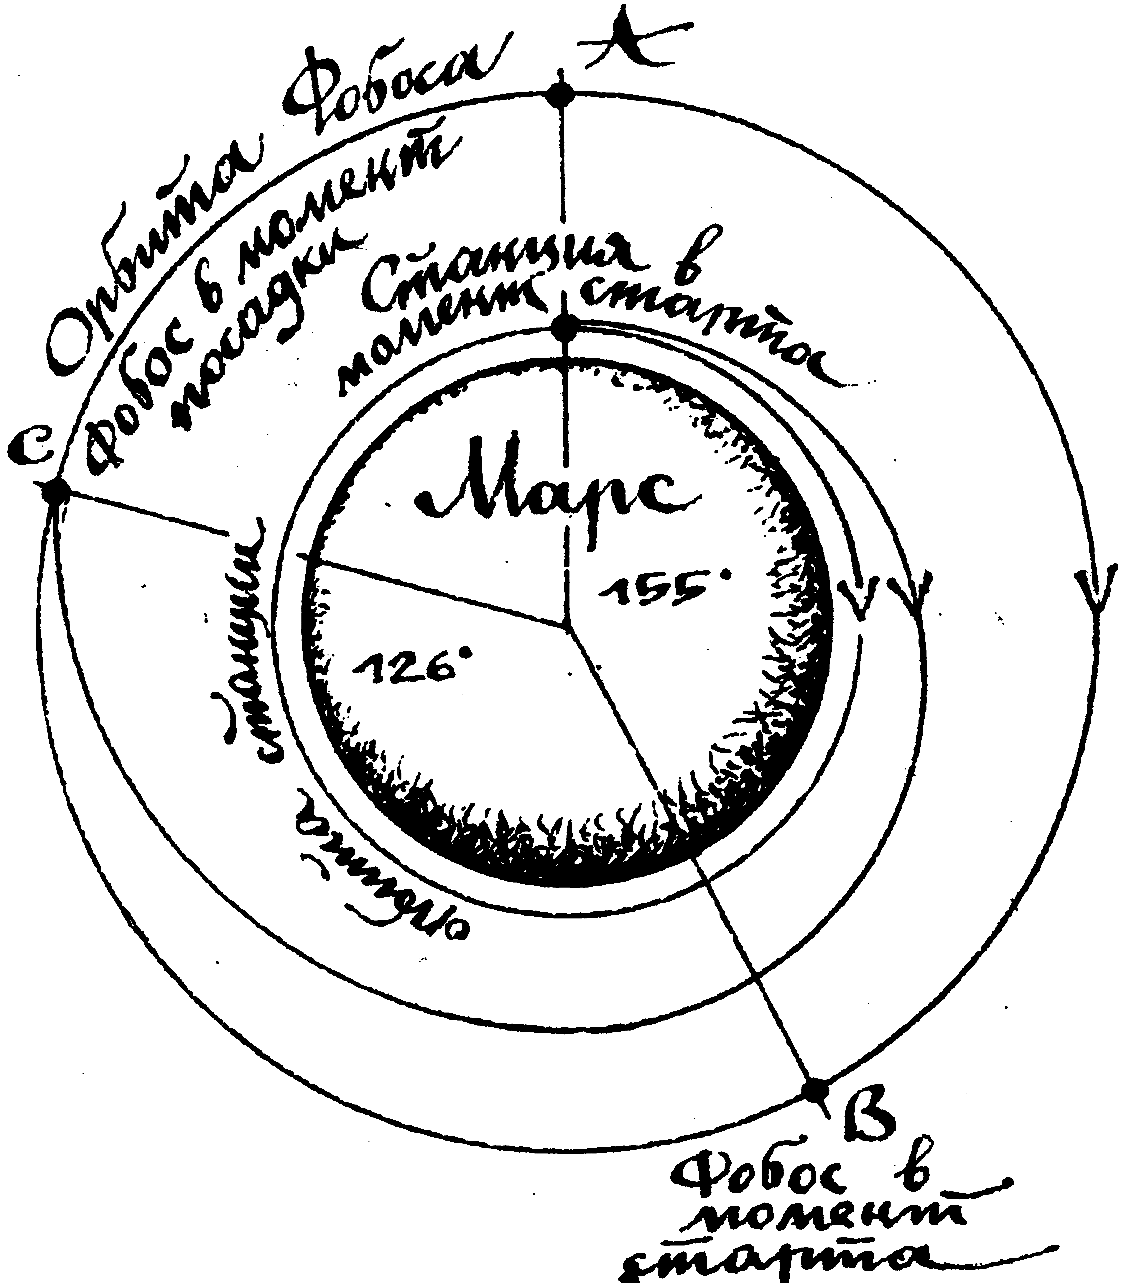
\includegraphics[width=0.5\textwidth]{fobos1}
\caption{Полет к Фобосу (по эскизу В. Ладохина).}
\end{figure}

\begin{figure}[H]
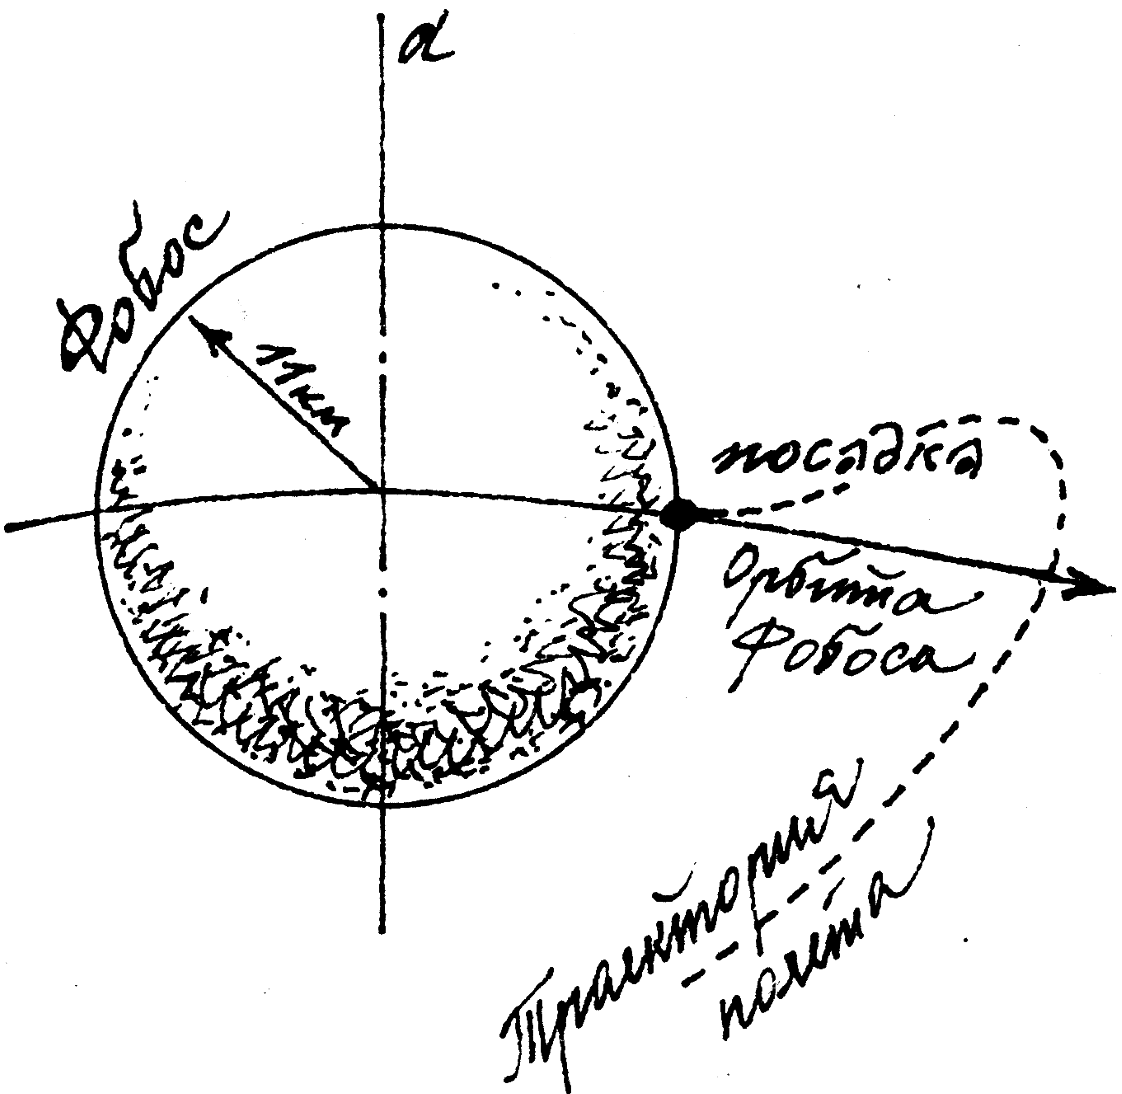
\includegraphics[width=0.5\textwidth]{fobos2}
\caption{Маневрирование в окрестностях Фобоса (по эскизу А. Артамонова).}
\end{figure}

Так проходит 1 час 25 минут, или 5100 секунд. Семнадцать раз по бесконечности. Открываю глаза и вижу сияющий шарик Фобоса. Он выглядит крупнее Луны. Осталось 815 км вверх и 609 вперед да скорости уравнять: сбросить излишек вертикальной (574 м/с) и скомпенсировать недостаток горизонтальной (—366 м/с). Ставлю рычаги на 200 кг за 6 с, угол тяги прежний, 90\degree. Два раза запускаю двигатель. Перегрузка вплотную приближается к трехкратной. Еще 200 кг: увеличиваю на секунду время маневра. Наконец последний импульс: 150 кг за 5 с. После отсечки двигателя отдыхаю 4 X 300 = 1200 с. Ровно двадцать минут. За это время горизонтальная скорость снижается до 96 м/с, вертикальная достигает 635. Будем гасить вертикальную: 180\degree, 150 кг, 6 с. Четырежды отправляю топливо в дюзы.

От 635 м/с остаются ничтожные 17 — всего 60 км/ч. А вверх идти 61 км. Пожалуй, маловато. Впрочем, как образно выражался наш инструктор по пилотажу, «не жалейте вертикальной скорости при подъеме, она скушает горизонтальную и поправит свои дела».

Что ж, можно опять отдохнуть. Тишина длится ровно четыре оборота стрелки бортового хронометра. По приборам скорости 62 и 81, расстояния 13 и 88 км — соответственно по вертикальной и горизонтальной осям координат. Опять пора гасить вертикальную скорость: 180\degree, 60 кг, 3 с. По завершении маневра разворачиваю суденышко вверх носом.

Серая, бугристая, покрытая мелкими «озерами» кратеров глыба Фобоса заполняет собою небо. Уже видны мерцающие огоньки посадочной площадки. Пора переключать аппаратуру в режим ближней навигации. Смотрю на часы: прошло еще три «пятиминутки». Но двигатель включать рано. Жду 20 секунд, потом еще 5. Рычаги стоят на 90\degree, 70 кг и 4,5 с. Остается нажать клавишу. Горизонтальная скорость зануляется, вертикальная равна 29 м/с. Ставлю 180\degree, 25,3 кг и 3,1 с и спустя 64 с даю импульс. Пока команда исполняется, передвигаю все три рычага. Новый рывок: 90\degree, 2 кг, 0,3 с. Тень лунолета бежит по неровной поверхности. Не проходит и минуты, как амортизаторы касаются грунта. Корпус кренится вперед, но шипы посадочных опор держат надежно.

Остается добавить для проверки, что всего на пульт было подано ровно 49 команд».

В тексте Л. Роканиди есть все необходимые цифры, он может служить проверочным тестом для программ ОС-1 и ОС-3. Вполне содержательные отчеты представили также Вадим Ладохин (Сургут), Павел Трубаев (Белгород), Сергей Свинолобов (Днепропетровск). Последний, кстати, вышел на старт позже других участников: МК-54 появился у него лишь в конце прошлого года. Однако после выполнения конкурсных заданий, а также дополнительного (перелет на станцию «ЮГ» с последовательным использованием программ ОС-1 и ОС-2) он был допущен к участию в перелете и быстро утвердился в лидирующей группе.

Надо сказать, что кое-кто из наших ведущих пилотов шагнул довольно далеко за рамки предлагавшегося задания. Так, десятиклассник Юрий Кузнецов из Куйбышева главный упор в отчете о полете «Тигриса» (так он окрестил свой корабль) сделал на историю около- марсианской базы «Галлей»: ее основой послужил астероид 2508 Алупка, открытый в 1977 году астрономом Н. Черных и после нескольких сближений с Вестой и Юпитером захваченный притяжением Марса. Решением Центрального Управления Космических Исследований, как сообщил Юрий, астероид переоборудовали в станцию. «Внутренняя часть использовалась как гигантский топливный бак вместимостью около 10 км$^{3}$, а оболочка, покрытая теплозащитным экраном, служила стартовой площадкой для космолетов, взлетающих или садящихся на Марс. Отсюда космические корабли направлялись к Фобосу, где дозаправлялись и продолжали полет».

«На зыбкой почве фантастики» согласно собственному чистосердечному признанию возвел здание своего «репортажа» грузчик-механизатор из Запорожья Александр Аула:

«— Вахтенный вычислитель, к капитану,— раздался по селектору голос старпома. Когда Байт, так звали молодого, подающего надежды вычислителя, вошел в ходовую рубку «Паруса», его ждали капитан, старпом и вахтенный пилот Лун Кор.

— Дружище Байт,— обратился капитан к вошедшему,— сделай расчеты прямого на Фобос и обратного полетов, эта часть программы нужна сегодня. Кроме того, после отхода «Кон-Тики» данные бортового вычислительного комплекса по радиоинтерфейсу держать в Большом Компьютере, чтобы в случае чего сразу выдать данные для коррекции.

— Слушаюсь, капитан, но в тени Марса возможны сбои,— ответил Байт.

— Сбоев не должно быть, Байт. Станция ОС-1 только что выведена на орбиту...»

И так далее. Правда, о самом перелете на спутник информации в «репортаже» Александра почти нет: гораздо больше внимания уделяется подготовке старта звездолета «Парус» в направлении Альфы Центавра. Тем не менее он отнесся к экспедиции на Фобос со всей возможной основательностью — слетал туда несколько раз, причем воспользовался на втором участке, помимо программы ОС-3, и программой «Лунолет-4»: это дало возможность оценить влияние собственного тяготения Фобоса на движение корабля. Как и следовало ожидать, оно оказалось очень незначительным.

Думается, что с эмоциональной стороной перелета на Фобос все более-менее ясно. Те же, кого в процессе посадки на этот спутник (и на другие небесные тела) больше интересуют физико-математические аспекты дела, могут найти довольно исчерпывающие сведения на этот счет в статье «Последний дюйм» (стр. 59).

Остается добавить, что на практике перелет со спутника на спутник впервые осуществили советские космонавты Леонид Кизим и Владимир Соловьев, успешно прошедшие 5—6 мая 1986 года на корабле «Союз Т-15» по маршруту: станция «Мир» — станция «Салют-7».

Кстати, первоначально корабль отставал от «Салюта»; перед космонавтами стояла примерно та же задача, какую решали читатели, догоняя станцию «ЮГ». И решена она была практически так же: торможение с последующим выходом в район станции. Операция, правда, заняла не один, а 16 витков — но и отставание было гораздо больше (3 тыс. км вместо 250 для «Кон-Тики»).

Многие читатели, интересующиеся в первую очередь нестандартными способами работы с ПМК, а также методами временного вывода машинки из строя, обращают внимание на «пустышку» (или «точку», как ее иногда называют), способ образования которой (Сх $\div$ ВП КНОП) был вскользь упомянут в № 12 за 1985 год.

«Эту точку можно даже записать в память,— делится опытом восьмиклассник В. Суворов из Свердловска,— и больше практически ничего. Даже не сложить 2+2, а в программной памяти вообще ужас! Можно делить на 0 — получится 0. Эта серия команд очень похожа на встречу автоматов с Тьмой: приборы выходят из строя, пленки засвечиваются и т. д.».

«Точка — сигнал капризный,— пишет восьмиклассник М. Рыжков из Новосибирска,— плохо записывается в память, лучше всего в регистр А. Сразу после формирования попробуйте перейти в режим ПРГ. Удивительная вещь! Счетчик шагов скачет совершенно произвольно, коды не соответствуют командам, иногда возникает вообще чепуха. Точку не так-то просто убрать. После Сх машина работает ненормально: не производит никаких действий, ни с того ни с сего начинает работать программа или машина вообще «уходит в себя», как йог. Вывести из этого состояния может лишь отключение».

«Посмотрите сами — не обрадуетесь,— резюмирует восьмиклассник из Москвы С. Банников.— Это неисправимо». «Не проходит ни одна команда... Караул! — вторит ему десятиклассник А. Степанов из Куйбышева.— ПМК не слушается, а может, он и слушается, но я ввел своей командой (точка) новый код».

Довольно детальный анализ представил П. Кузнецов из Ленинграда: «Точки. Это название я дал по их типичному представителю (Сх К7 ВП КНОП). «Точки» вообще (та же операция над несколькими нулями), попросту говоря, пустое место на месте (каламбур) первой значащей цифры мантиссы. Разновидности точек можно получить командой 1/х от чудовищ- хвостов ОС-оборотней (только от них) — «ненормальный» случай, так как должна вроде бы получиться Тьма: 1000—430=570, уровень Тьмы. Точки очень коварны — пока они находятся в стеке, многие команды не выполняются или коверкаются. Программирование лучше в это время не включать — программа будет испорчена, а на индикаторе будет твориться черт-те что: режим ПРГ выйдет из строя. Если же особенно долго измываться над точкой, то в режиме ПРГ это будет уже не временно, а постоянно и ПМК придется выключить. Точки также имеют привычку «сбегать» — могут перемещаться из одного регистра в другой, сдвигая заодно за собой по кругу содержимое остальных регистров и вызывая по ходу передвижения некоторые побочные явления. Это свойство точек было бы очень ценно, если бы они не портили программу. А так как такое передвижение в регистрах все равно возможно, то почему бы разработчикам ПМК не сделать его осуществимым специальными командами в следующих моделях?»

И действительно, почему бы? Но вернемся к своей БЗ-34 (МК-54). У каждого отрицательного явления есть свои плюсы. Есть они и у «пустышки». Кстати, П. Кузнецов прав: имеет смысл говорить о целом классе таких объектов: если процесс формирования начать не с нуля, а с нескольких (например, Сх 000 $\div$ ВП КНОП), получим «пустышки», завершающиеся несколькими нулями (в данном случае двумя). Наиболее «опасны» самые «старшие» из них (получившиеся из семи либо восьми нулей); с ними то, о чем пойдет речь, не проходит. Зато все остальные сойдут вполне.

Для начала сформулируем алгоритм полной «ликвидации» таких объектов: при появлении на индикаторе «пустышки» нужно семь раз подряд нажать стрелку вверх. Стек полностью очищается. А теперь займемся делом.

Как известно, в регистры БЗ-34 можно записать лишь 14 чисел. Так вот, «пустышка» позволяет запомнить еще три (правда, не всяких — подходящие числа ограничены как по порядку, так и по длине мантиссы).

Запишем для начала в регистр 9, скажем, число 111111 (шесть единиц). Затем по стандартному алгоритму получим любую из «младших» пустышек. Теперь нужно нажать стрелку вверх, ИП9 и еще пять раз стрелку вверх. «Пустышка» ликвидирована, а число 111111 куда-то записано (но куда, никому не известно).

Повторим ту же процедуру еще дважды, записав в первом случае в регистр 9, скажем, число 222222 (шесть двоек), а во втором — 333333 (шесть троек). «Пустышка», фигурирующая в каждой операции, может быть любой, но обязательно из «младших». По завершении операции все три числа (111111, 222222 и 333333) оказываются куда-то записаны!

После «ликвидации» последней «пустышки» можете смело вводить в свой ПМК любую сколь угодно сложную программу, использующую подпрограммы, циклы, команды косвенной адресации, занимающую все ячейки памяти и использующую все адресуемые регистры. Поработав с ней хоть целый день, сформируйте какую-нибудь «пустышку» (из «младших») и примените к ней алгоритм «ликвидации». Вы увидите на индикаторе последовательно два из записанных чисел: 222222 и 111111. А если вместо алгоритма «ликвидации» дважды нажать \XY, глазам предстанет другая пара: 333333 и 222222.

Администрация КЭИ обычно использует этот способ для запоминания шестизначных телефонных номеров (семизначных удается записать только два).

Еще об одном полезном свойстве «пустышки» рассказывает наш постоянный корреспондент Дмитрий Кайков из Белгорода:

«Используя точку, можно получать и шифры. Сделаем вот что: 10 F1/x ПА Сх $\div$ ВП ПД ИПА П0 1 П0 П0 ПВ. Теперь нажмем «сброс» (Сх) и, нажимая на стрелку вверх, будем сбрасывать все появляющиеся числа. Теперь вызовем из регистра В код 01 30. Можно избавиться от порядка: ВП /—/ 30 ПВ. Этот код (01) можно использовать в программе. Оператор /—/ меняет ноль в самом левом разряде на L. Поманипулировав операторами КИП, ВП, /—/ и т. д., можно получать разные другие коды (например, применив к исходному сообщению 01 последовательность /—/ П0 КИП0 ИП0, получим L-------0. Только стоит внимательно и осторожно обращаться с кодами, у которых второй разряд (я считаю слева, включая и самый первый) пуст. Такой код, например, можно получить из 01, записанного в регистре В (или любом другом) командой КИПВ. Этого шифра и ему подобных, как и «точки», следует опасаться, так как может произойти путаница в программной памяти и даже в стеке».

Если у кого-нибудь есть информация о еще каких-то полезных применениях «пустышки» и родственных ей символов, просим дать знать.

Михаил ПУХОВ

\section{ПОСЛЕДНИЙ ДЮЙМ}
«Все дело в том, чтобы правильно рассчитать,— сказал Бен.— Когда выравниваешь самолет, надо, чтобы расстояние до земли было шесть дюймов. Не фут и не три, а ровно шесть дюймов! Если взять выше, то стукнешься при посадке и повредишь самолет. Слишком низко — попадешь на кочку и перевернешься. Все дело в последнем дюйме...»

Легко догадаться, что наше очередное занятие не случайно открывается цитатой из хрестоматийного рассказа Джеймса Олдриджа. Разговор пойдет об алгоритмах посадки. А поможет нам, как обычно, посадочный модуль, изготовленный художником Евгением Катышевым.

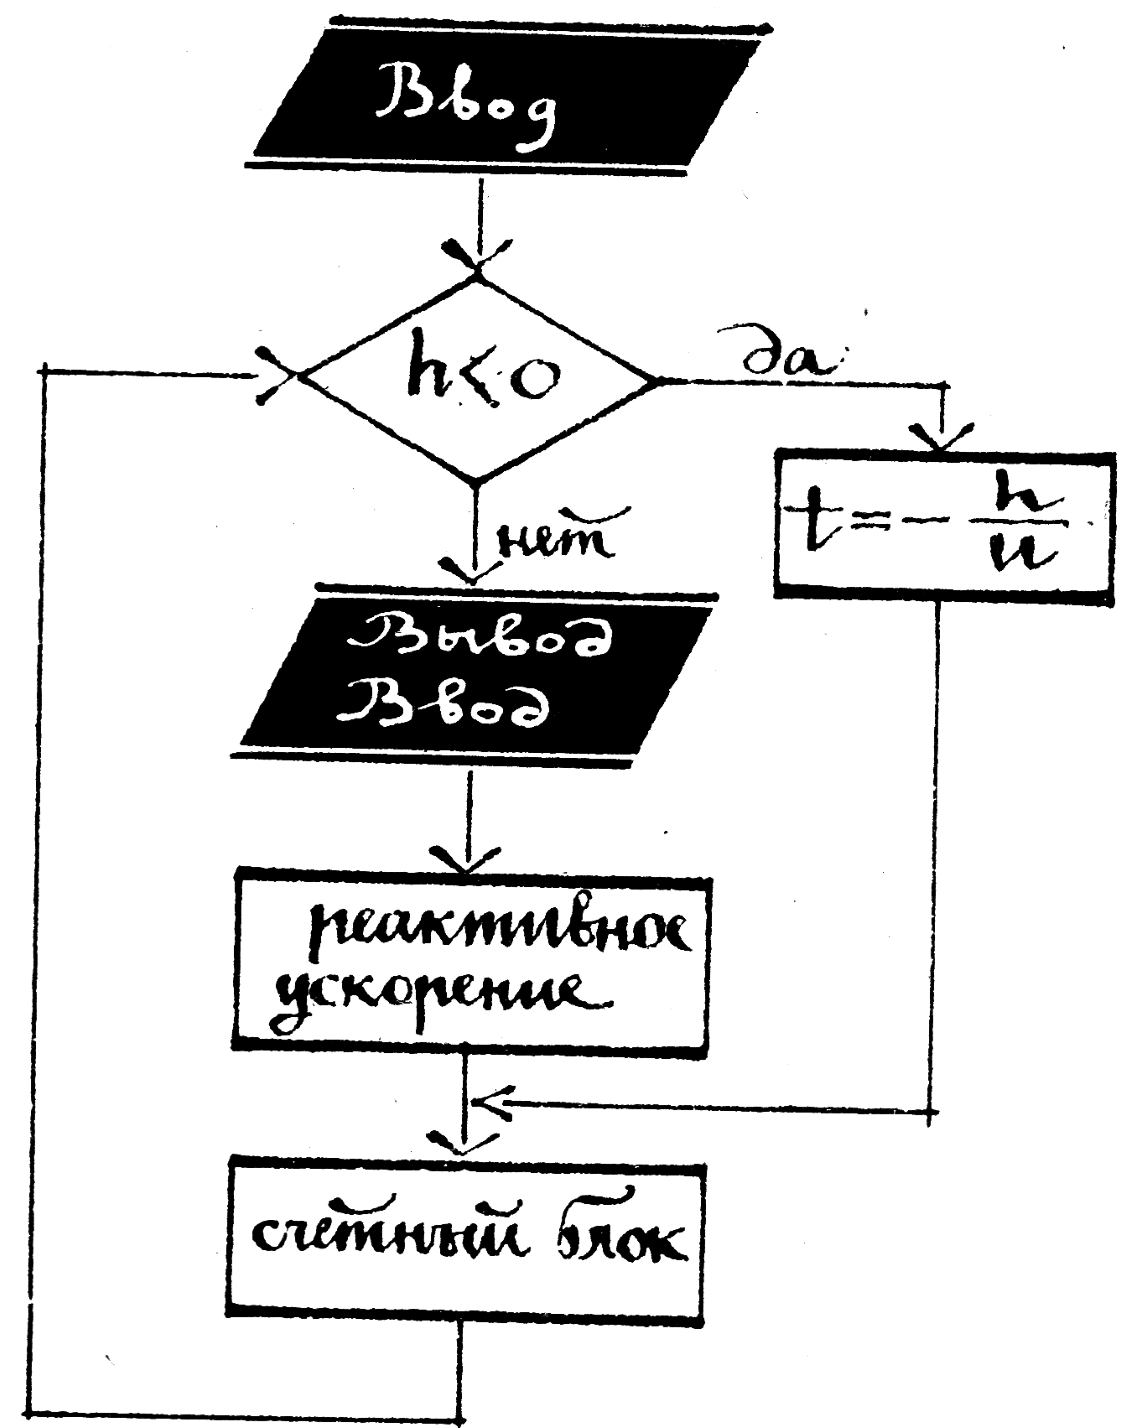
\includegraphics[width=0.5\textwidth]{last_d1}
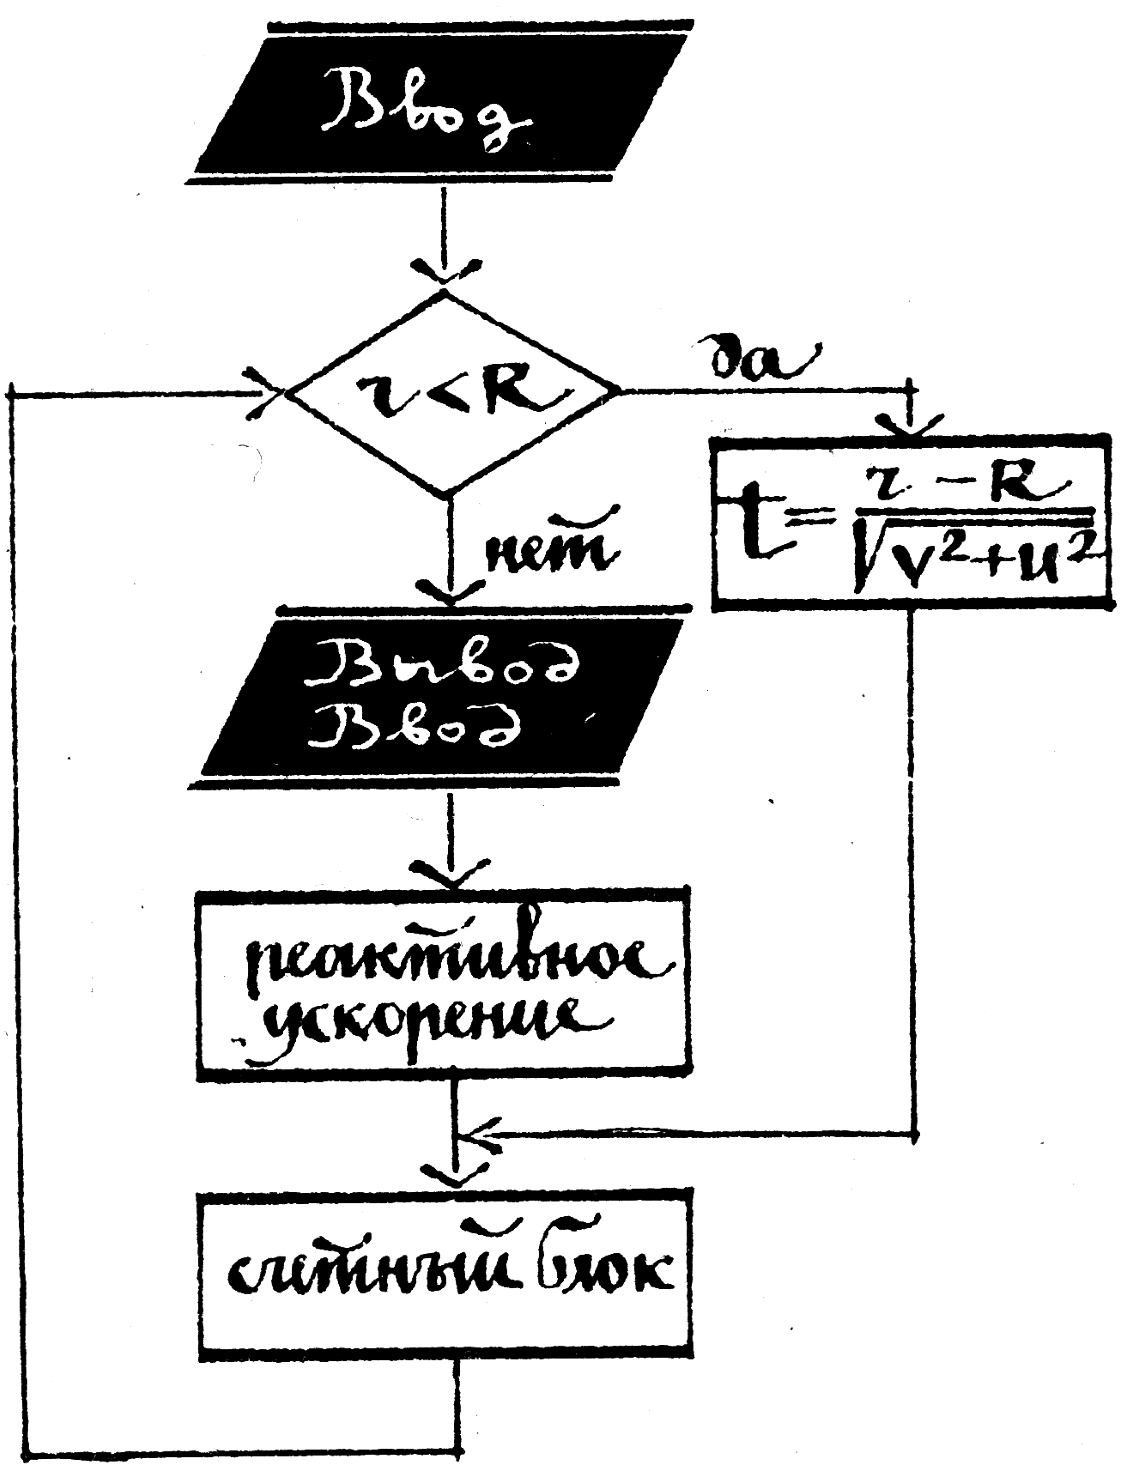
\includegraphics[width=0.5\textwidth]{last_d4}

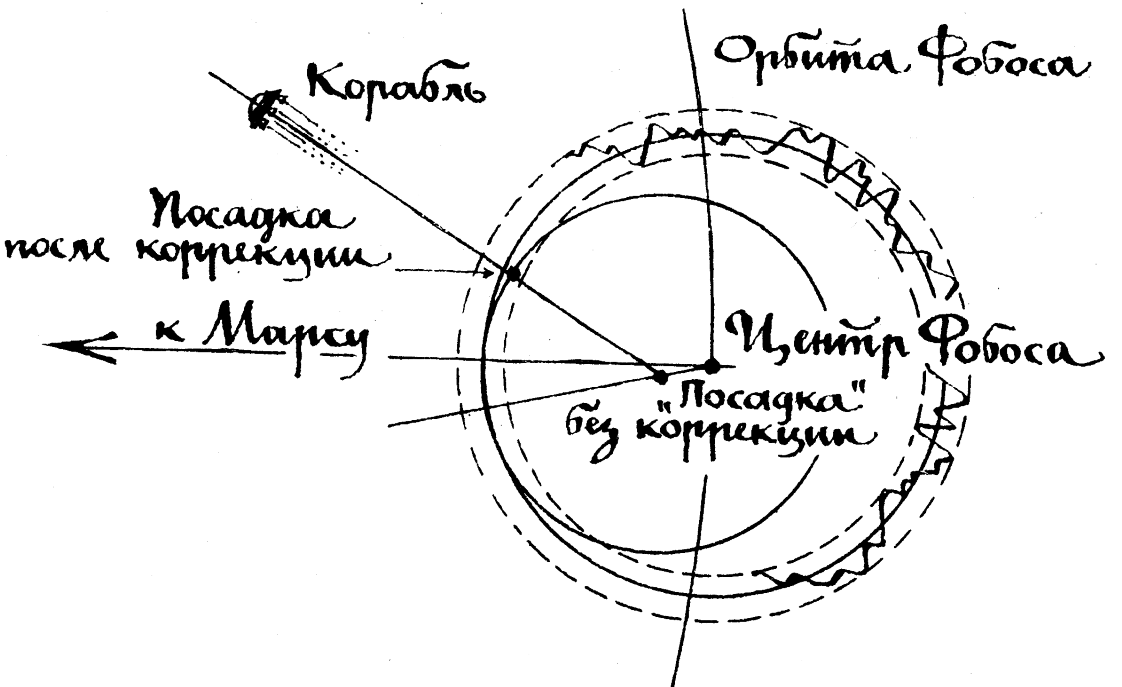
\includegraphics[width=0.5\textwidth]{last_d2}
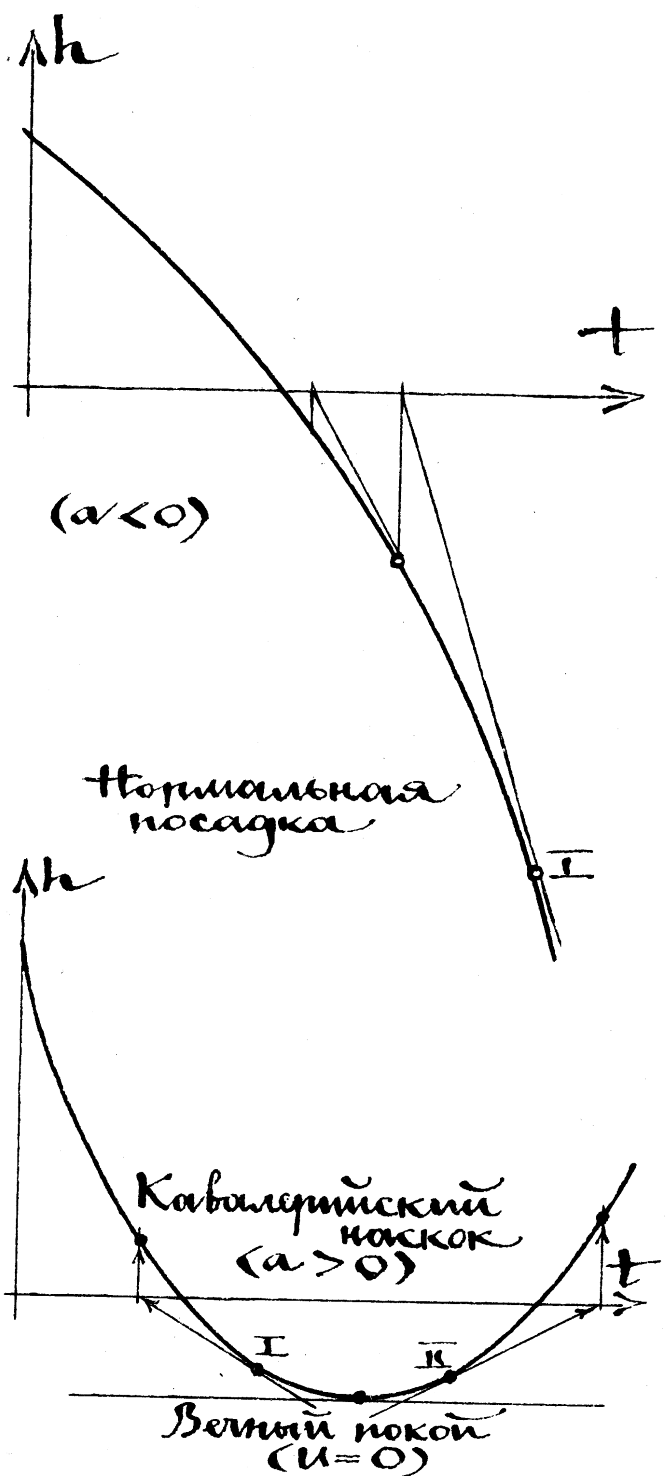
\includegraphics[width=0.5\textwidth]{last_d3}

Итак, первое упражнение — «приземление» на планету достаточно большую, чтобы можно было пренебречь ее шарообразностью и считать плоской. Теперь обратимся к блок-схеме алгоритма. Прежде всего вводятся исходные данные — характеристики планеты и корабля, начальные значения переменных. Затем следует блок сравнения. В момент старта высота, конечно, неотрицательна (выход из ромба по стрелке «нет»), и настает пора брать в руки штурвал — задавать значения управляющих параметров. После этого включаются блоки определения реактивного ускорения и вычисления переменных: их устройство известно по предыдущим выпускам (см. «ТМ» № 5, 6 за 1986 год). Полученные результаты выводятся на индикатор, но предварительно проверяется высота. Пока полет проходит вдали от поверхности, никаких проблем не возникает, ведь «все дело в последнем дюйме». Но если ошибка летчика в момент приземления может оказаться роковой, то наш бортовой компьютер корректирует действия экипажа. Как же это происходит?

Проанализируем алгоритм посадки на последнем маневре. Если вам удалось, снизившись почти до поверхности, погасить скорость летательного аппарата, то проще всего либо совсем выключить двигатель, либо малой тягой частично скомпенсировать силу тяжести, чтобы суммарное ускорение было направлено вниз. Лунолет падает с небольшой высоты, и его вертикальная скорость попросту не успевает выйти за допустимые пределы.

Подобрать время финального маневра так, чтобы в момент его завершения высота в точности обратилась в нуль, затруднительно. Скорее всего аппарат «заглубится» в поверхностные слои планеты. В этом случае мы выходим из блока проверки по стрелке «нет» и микрокалькулятору надо подкорректировать посадку. С методом коррекции путем половинного деления мы уже знакомы (см. «ТМ» № 6 за 1986 год). Обсуждаемый сегодня способ отличается существенным (особенно для ПМК) достоинством — он работает («сходится») гораздо быстрее.

Как и в прошлом выпуске, наш электронный помощник играет роль своеобразной машины времени, возвращающей аппарат по траектории назад, в точку касания с поверхностью. Разделив высоту на вертикальную скорость (та и другая отрицательны) и поменяв знак полученного числа, он находит отрицательное время «шага назад», подставляет его в уравнения движения и подтаскивает лунолет ближе к поверхности. За один шаг выбраться из «подземелья» обычно не удается (см. график зависимости высоты от времени, случай «нормальная посадка»). 

Поясним, в чем дело. Для тех, кто знаком с понятием производной, не составит труда доказать, что в любой точке тангенс угла наклона касательной к кривой h(t) равен значению вертикальной скорости в этот момент времени. Поэтому геометрически алгоритм можно иллюстрировать так — в той точке, где оказался аппарат в результате последнего маневра, к графику проводится касательная, пересечение ее с временной осью и определяет величину «шага назад». Из графика видно, что мы пока еще остались под поверхностью небесного тела. (Выйти за один шаг можно только в случае прямолинейного графика, то есть равномерного спуска.) Теперь цикл повторяется — так как высота отрицательна, то из блока проверки мы опять выходим по стрелке «нет» и снова делаем «шаг назад». И так далее. В результате всего за несколько шагов высота (в пределах заданной точности) обращается в ноль — лунолет на поверхности, а уж в каком состоянии, это зависит от скорости.

«Цель расчетов не число, а понимание»,— утверждают многие математики. Если посмотреть на наш алгоритм с этой точки зрения, то нетрудно увидеть, что фактически мы приближенно решили уравнение h(t)=0. Следует признаться: описанный процесс придуман давным-давно и носит название «метода касательных». Надеемся, он пригодится читателям и при решении других задач.

Наряду с осторожными космолетчиками встречаются у нас в КЭИ и любители острых ощущений. Их стиль пилотирования — маневры с предельными перегрузками, «полет на грани реанимации». Если корабль космического лихача окажется «под землей», то коррекция приводит к неожиданным результатам (случай «кавалерийский наскок»). Хотя метод остался прежним (личные качества пилота калькулятором не учитываются), вид кривой h(t) изменился. Если теперь сделать «шаг назад», то мы окажемся не под, а над поверхностью планеты. Корабль как бы подбросило вверх (см. «ТМ» № 3 за 1986 год). Посовещавшись, мы решили назвать это явление «эффектом пороховой бочки» (ЭПБ) — в самом деле, представьте себе, что вы, дав полную тягу, пытаетесь приземлиться на площадку, вымощенную толовыми шашками.

Возможен и другой случай. Если аппарат проскочит вершину параболы, то «шаг назад» сменится «шагом вперед». Корабль как бы «рикошетирует». Те, кто сажал «Кон-Тики» в океан, возможно, уже столкнулись с этим явлением.

Наконец, может получиться так, что в результате посадочного маневра аппарат окажется в точке «вечный покой». Вертикальная скорость при этом равна нулю и при попытке деления на индикатор выводится сигнал ошибки — лунолет навечно погребен в недрах планеты, обратной дороги нет.

А теперь второе упражнение — посадка на сферическое небесное тело сравнительно малых размеров. Поверхность его может иметь неровности: посадка считается завершенной, если отклонение от средней поверхности шара не превышает некоторой, заранее заданной величины (в программе «ОС—3»— 1 м).

Если в результате маневра корабль оказался внутри сферы (точка «посадка без коррекции»), то ПМК определяет кратчайшее расстояние до поверхности и, разделив его на модуль скорости, делает «шаг назад», а в случае необходимости и несколько. В ситуации, изображенной на рисунке, достаточно однократной коррекции.

Описанные в этом и предыдущих выпусках способы коррекции посадки, по сути дела, представляют собой различные методы решения уравнений. В зависимости от применяемого варианта возникают дополнительные физические эффекты (ЭПБ, рикошет). С другой стороны, решая ту или иную задачу, важно умело выбирать математический аппарат, чтобы наиболее полно учесть все существенные факторы. Собственно, искусство программирования и состоит в построении наиболее точной модели и алгоритмизации изучаемого процесса, а сама программа — это, как говорится, дело техники, правда, порой довольно виртуозной.

«Последний дюйм, который разделяет всех и вся, нелегко преодолеть, если не быть мастером своего дела. Но быть мастером своего дела — обязанность летчика». Эти слова Дж. Олдриджа можно адресовать представителям любой профессии.

Сергей ВОЛКОВ,

инженер

\section{ПОЕДИНОК С РОБОТОМ}
«Колоссальные захваты приближались... вот они загородили все небо... сомкнулись на корпусе «Кон-Тики»... И вдруг... («ТМ» № 11 за 1985 г.)

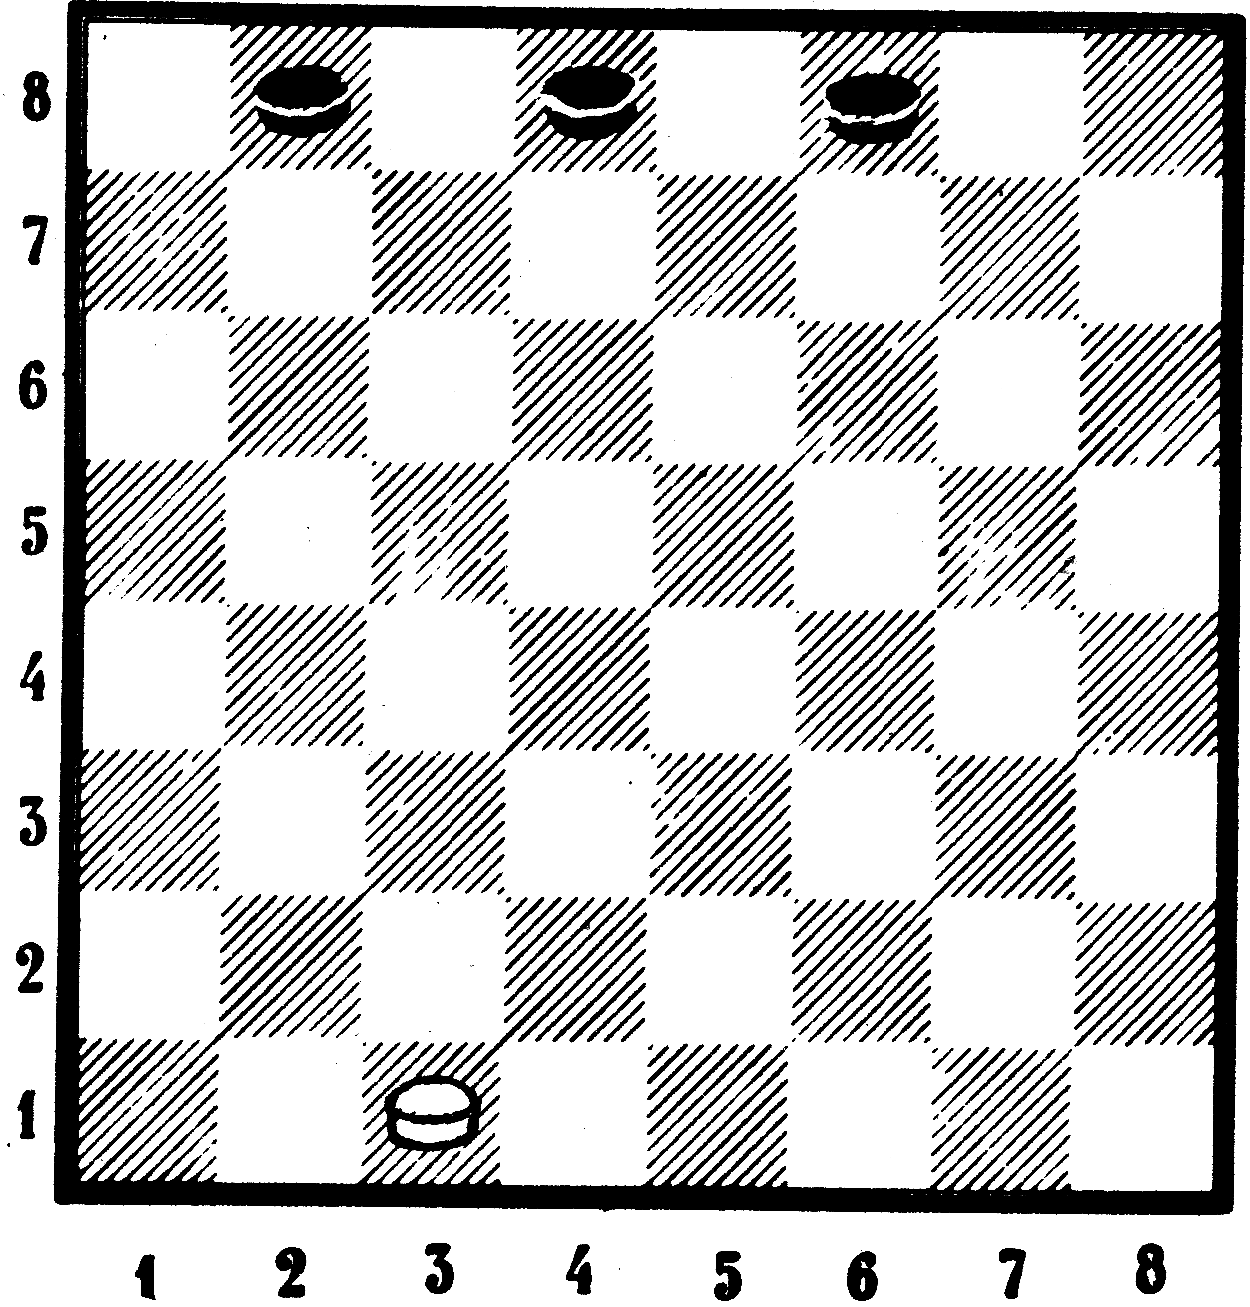
\includegraphics[width=0.5\textwidth]{fight_with_robot}

Несомненно, многие наши читатели, рискнувшие выполнить задание по облету станции «ЮГ» в легоньком скафандре, с миниатюрным ракетным двигателем за спиной, на собственном горьком опыте убедились в дурном нраве механического чудовища, охраняющего станцию от «непрошеных гостей». Те, кого интересует конструкция этого не особо вежливого автомата, ошибочно принятого М. Коршуновым за «причальный манипулятор», могут детально познакомиться с ней в разделе «Алгоритмическая гимнастика». Пользуясь случаем, напомним, что первым в истории космонавтики «всамделишным» причальным манипулятором, как известно, оборудована советская орбитальная станция «Мир».

Страж станции «ЮГ», как помнят читатели, не был единственным роботом, в поединок с которым вступили отважные путешественники. До него был кофейный «однорукий бандит», после — «робот-бюрократ», в перепалке с которым А. Перепелкин невольно заложил фундамент грядущей победы. Но некоторые читатели, в частности Г. Горовой из Керчи, не без основания подозревают, что на протяжении всего героического перелета в кабине «Кон-Тики» незримо присутствовал и третий участник — бортовой компьютер. И не может быть, чтобы А. Перепелкин и М. Коршунов не сражались бы с ним постоянно. Разумеется, на нашем излюбленном поприще электронных игр.

Следует честно признаться: так оно и было. Наиболее тяжкие случаи злоупотреблений азартными играми наблюдались на участке «точка либрации — Земля», а также после приводнения, когда свободного времени у наших героев было хоть отбавляй. И сразу откроем второй секрет: хотя бортовая игротека «Кон-Тики» была весьма обширна, наибольшей популярностью среди экипажа пользовались шахматы, шашки, «уголки» и прочие традиционные игры на стандартной квадратной доске 8X8.

Но какая связь между ними и нашей скромной «Электроникой»?

«Недавно у меня возник вопрос, и я хотел бы проконсультироваться с вами,— пишет В. Ревуцкий из Киева.— Можно ли использовать микрокалькуляторы «Электроника БЗ-34», «Электроника МК-54», «Электроника МК-56» для игры в шахматы или решения некоторых шахматных задач. Если можно, то напечатайте, пожалуйста, программу для этого».

Как видим, у отдельных читателей возникла не вполне обоснованная вера во всемогущество ПМК. Какие там шахматы! Какие шашки! Вообще любая стратегическая игра на шахматной доске покажется абсурдом почти всякому, кто хоть раз в жизни видел Б3-34 (МК-54). Одних только клеток 64 — разве их все упомнишь? А фигуры? А осмысленную стратегию как задавать? Случайным образом? Пиши пропало, ходи как попало — где наша не пропадала?! Так, что ли?

Но не будем горячиться. Заглянем лучше еще в одно письмо — от нашего постоянного корреспондента, студента-первокурсника Дмитрия Кайкова из Белгорода.

«А теперь я хочу рассказать вам о еще одной своей «мыслящей» программе. Есть такая игра — тремя или четырьмя шашками надо прижать одну шашку противника к краю шахматной доски, чтобы та не могла сделать ни одного хода («волки» ловят «серенького козлика»). «Козлик» (белая шашка, которой «руководит» калькулятор) может ходить как вперед, таки назад (по черным клеткам), а «волки» (их направляет человек) только вперед. Ни «есть», ни перепрыгивать через шашки никому нельзя. Калькулятор стремится прорваться сквозь строй «волков», а те как уже было сказано, стремятся поймать его в ловушку.

00.КПП7 01.КИП8 02.5 03.0 04.- 05. Fx<0 06.19 07.КППА 08.КИП8 09.2 10.0 11.- 12.Fx$\geq$0 13.28 14.КППВ 15.КППС 16.КППД 17.ИП9 18.Кх<о7 19.КППВ 20.КИП8 21.8 22.0 23.- 24.Fx<0 25.16 26.КППА 27.КППД 28.КППС 29.БП 30.17 31.КИП8
32.1 33.1 34.+ 35.ИП9 36.Fx<0 37.41 38.\XY
39.П5(6) 40.\XY 41.\XY 42.4(5) 43.П0 44.\XY
45.$\uparrow$ 46.$\uparrow$ 47. КИП$\uparrow$ 48.- 49.Fx$\neq$0 50.97 51.\FO 52.FL0 53.47 54.5(6) 55.П8 56.ИП9 57.1 58.+ 59.П9 60.Fx$\neq$0 61.01 62.ИП5(6) 63.П4(5)
64.с/п 65.П9 66.с/п 67.КП9 68.КБП0 69.КИП8 70.9 71.- 72.БП 73.35 74.КИП8 75.9 76.+ 77.ИП9 78.Fx<0 79.41 80.\FO 81.2 82./-/ 83.П9 84.БП 85.38 86.КИП8 87.1 88.1 89.- 90.БП 91.77 92.4(5) 93.П8 94.1 95./-/ 96.П9 97.в/о

Вот программа этой игры на языке БЗ-34. Для начала пронумеруем черные шашки (их три) и вместо букв на доске (по горизонтали) поставим цифры, как на рисунке. Теперь каждой клетке соответствует двузначное число: первая цифра — это координата по горизонтали, вторая — по вертикали. Пусть в начальной позиции «волки» занимают клетки 28, 48 и 68 (это задается командой 28 П1 48 П2 68 ПЗ), а «козлик» — позицию 31 (31 П4). В ходе игры в этих же регистрах будут храниться текущие координаты шашек. Перед игрой надо в некоторые регистры записать адреса переходов: 92 П7 31 ПА 69 ПВ 74 ПС 86 ПД.

«Козлик» ходит первый. Нажимаем В/О С/П. Через 35 с на индикаторе загорается 42 — ПМК двинул свою шашку на это поле. Теперь наш ход. Для этого набираем номер шашки, которой хотим пойти (скажем, 1), С/П, номер клетки, куда идем (допустим, 37), и снова С/П. Калькулятор фиксирует этот ход, делает ответный, и все повторяется. Программа может использоваться и для четырех «волков». Для этого достаточно записать по адресам 39, 42, 54, 62, 63 и 92 цифры, данные в скобках. Координаты «волков» в таком варианте хранятся в регистрах 1—4, «козлика» — в регистре 5.

Надо сказать, что из-за малого объема программной памяти калькулятор просматривает ситуацию максимум на два хода вперед, поэтому иногда действует «не очень логично». Но тем не менее даже я сам у него не выиграл ни разу. (Очевидно, в варианте 3:1; с четырьмя «волками» выиграть нетрудно.— М. П.) Программа работает следующим образом: сделано так, что белая шашка стремится быть всегда у осевой линии поля (между 4-й и 5-й вертикалями). Сначала определяется, на какой половине поля находится «козлик» (адреса 01-06). Если слева— управление передается на участок программы с начальным адресом 07, если справа — с адресом 19. Да, до этого в регистр 8 автоматически записывается четверка, в регистр 9 — единица с минусом (адреса 00, 92-97). Для производства ходов вправо-вперед, влево-вперед, вправо-назад и влево- назад служат подпрограммы ППА, ППВ, ППС и ППД соответственно (в регистрах А, В, С и Д хранятся адреса их первых команд). В приведенном примере первой срабатывает ППА: калькулятор «мысленно» делает ход вправо- вперед и заносит результат в регистр 5. Начиная с адреса 42, производится опрос координат «волков» и «козлика» (регистры 4 — 1). Если позиция одного из них совпадает с содержимым регистра 5, то такой ход невозможен, сработает В/О, и калькулятор с помощью следующей подпрограммы примется за обдумывание другого хода. Если же путь свободен, то произойдет перекодировка регистра 8 и 9 (фрагмент 54—59), затем произойдет переход на адрес 01.

Теперь «Электроника» начинает думать дальше: а не идет ли она в ловушку? Для этого производится проверка — есть ли хотя бы один выход из того положения, в которое она попадет, если сделает намеченный ход. Происходит это по тому же алгоритму. Если найдется хоть одна соседняя пустая клетка, куда «козлик» мог бы в случае чего выскользнуть, то ПМК пойдет на поле, координаты которого записаны в регистре 5 (фрагмент 56-59 и 60-64). Теперь, кстати, ясно, зачем проверяются координаты самого «козлика» — ведь одну из возможных клеток после второго хода занимает он сам. Если же пустой клетки не окажется, то в регистры 8 и 9 снова занесутся исходные числа, и калькулятор примется за другую клетку.

В программе есть ограничивающие (не знаю, как их еще назвать) «участки» по адресам 08-13 и 20-25, которые следят, чтобы «козлик» не вышел за правую и левую границы поля.

Если ПМК не может пойти вперед, то наступает очередь подпрограмм ППС (начальный адрес 74) и ППД (86). Теперь «Электроника» пойдет в клетку сразу же, если только та пуста. Это обеспечивает фрагмент 77-85.

Время работы 35—150 с.».

Программа Д. Кайкова (играть с ней, кстати, весьма интересно: создается четкое впечатление, что действиями «козлика» руководит вдумчивый, осторожный противник) , пожалуй, посложнее тех, с которыми мы имели дело раньше. В основном это связано с широким использованием косвенной адресации. В основном она используется для экономии программной памяти: например, команда КППА эквивалентна паре ПП 31 (в регистре А хранится число 31). Команда КБП0, записанная по адресу 68, эквивалентна БП 00: к тому моменту, когда управление переходит к ней, в регистре 0 находится единичка, а при косвенном обращении она модифицируется: 1-1=0, закон природы! Наконец, по адресу 47 записана «нештатная» (для БЗ-34) команда КИПЕ: действует она в данной ситуации точно так же, как и в программе «Мультфильм» (разъяснения по этому поводу см. «ТМ» № 4 с. г.).

Кстати говоря, именно из-за этой команды программа Д. Кайкова в приведенном виде непригодна для непосредственного использования на ПМК «Электроника МК-61» — связь регистров 0 и Е в этой модели, как мы знаем, разорвана. Конечно, возможности МК-61 гораздо больше, но... «Обращаемся к вам в связи с возникшими трудностями в работе с МК-61,— пишут, например, студенты Р. Марьянов и А. Яланский из Запорожья.— В данной модели введен регистр Е, что затрудняет использование для него программ, составленных для предыдущих моделей. В частности, работая с программой «Городки» («Наука и жизнь» № 4 с. г.), мы столкнулись с фактом отказа работы калькулятора. (Далее в письме приводится фрагмент программы.— М. П.) Нам кажется, что ошибка допускается на шагах 02-04. Мы воспользовались советом вашего журнала по установлению искусственной связи регистров Е и 0, но ожидаемых результатов не получили».

Напомним: в нашей рекомендации говорилось, что установление такой связи требует минимум двух команд ИП0 ПЕ. В некоторых случаях этого действительно достаточно. Но чаще для нормальной работы требуется еще и восстановить стек. Как правило, для этого достаточно команды круговой передачи (код 25), вписанной сразу же после двух приведенных. А иногда (как в программе Д. Кайкова) можно обойтись и командой \XY.

К счастью, в предлагаемой игре имеются «внутренние резервы»; иными словами, программу можно сократить на несколько команд. Это позволяет дать вариант, одинаково пригодный как для БЗ-34, так и для МК-61. Нужно заменить участок по адресам 45-66 на следующий:

45.ИП0 46.ПE 47.\XY 48.КИПЕ 49.- 50. Fx$\neq$0 51.97 52.FBx 53.+ 54.FL0 55.45 56.5(6) 57.П8 58.ИП9 59.1 60.+ 61.П9 62. Кх$\neq$0Е 63.ИП5(6) 64.П4(5) 65.С/П 66.П9

Изменяется только способ ввода очередного хода. Теперь нужно набрать номер шашки, затем ПП и номер поля. Впрочем, такой ввод хорошо знаком нам по прошлым программам. Владельцы Б3-34 (МК-54) должны помнить, что буква Е по адресам 46, 48, 62 соответствует на их клавиатуре стрелке вверх. Цифры в скобках, как и раньше, дают «вариант 4 волков».

Михаил ПУХОВ

\section{ПОЕЗДКА НА «ЮГ»}
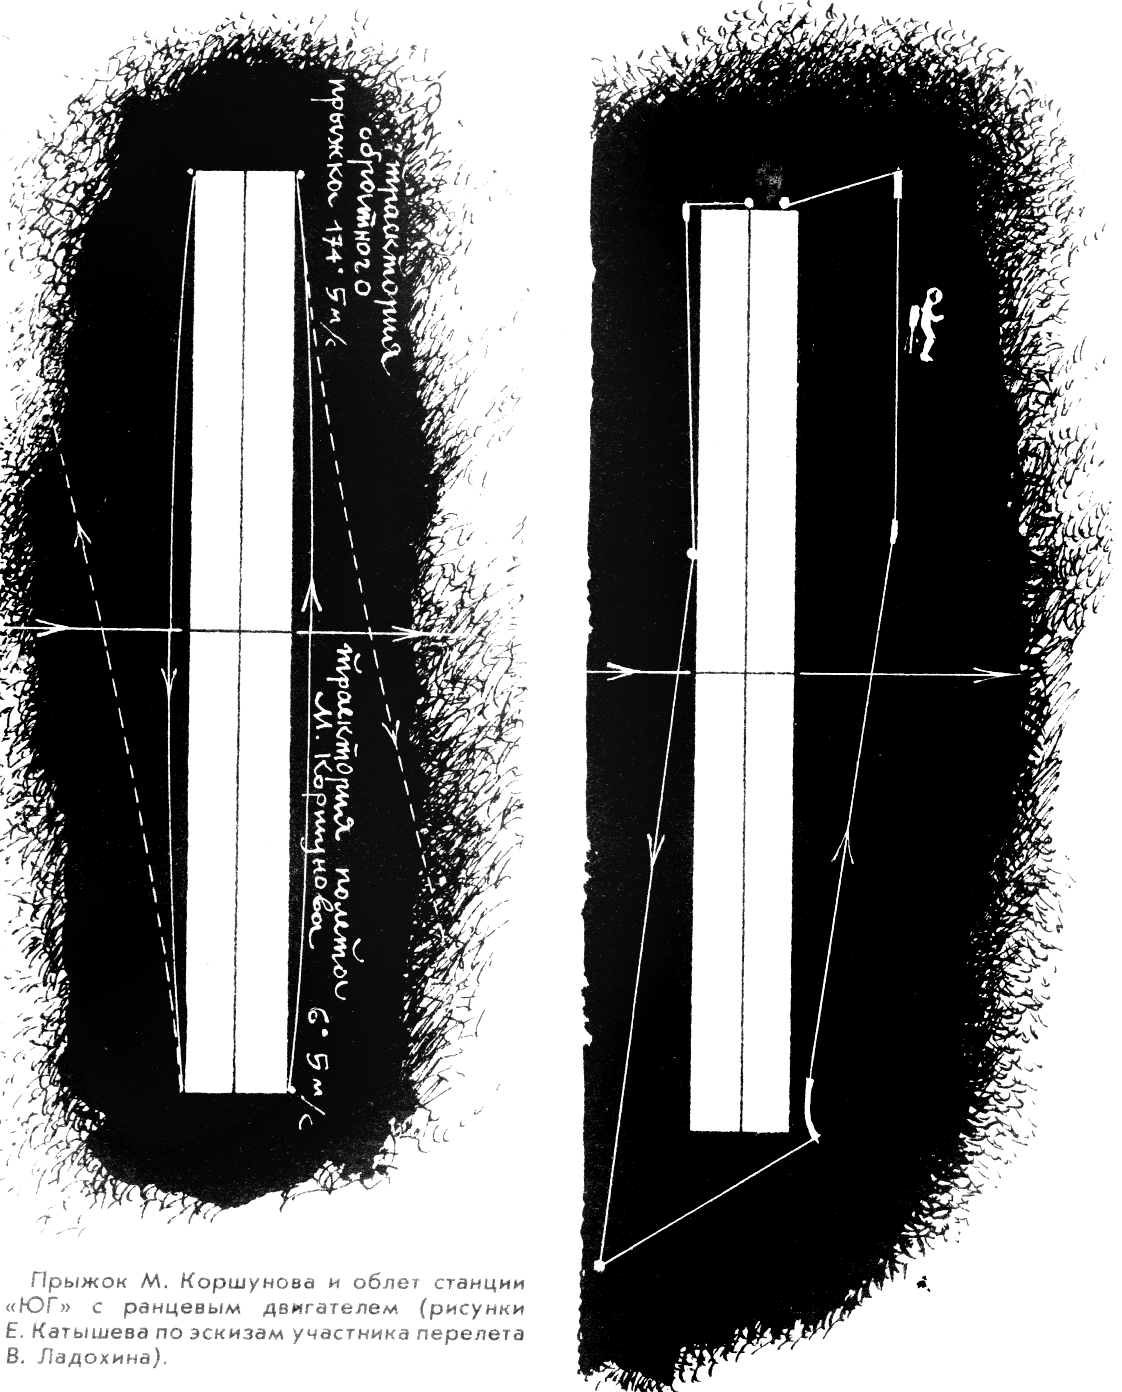
\includegraphics[width=0.5\textwidth]{jump_to_ug}
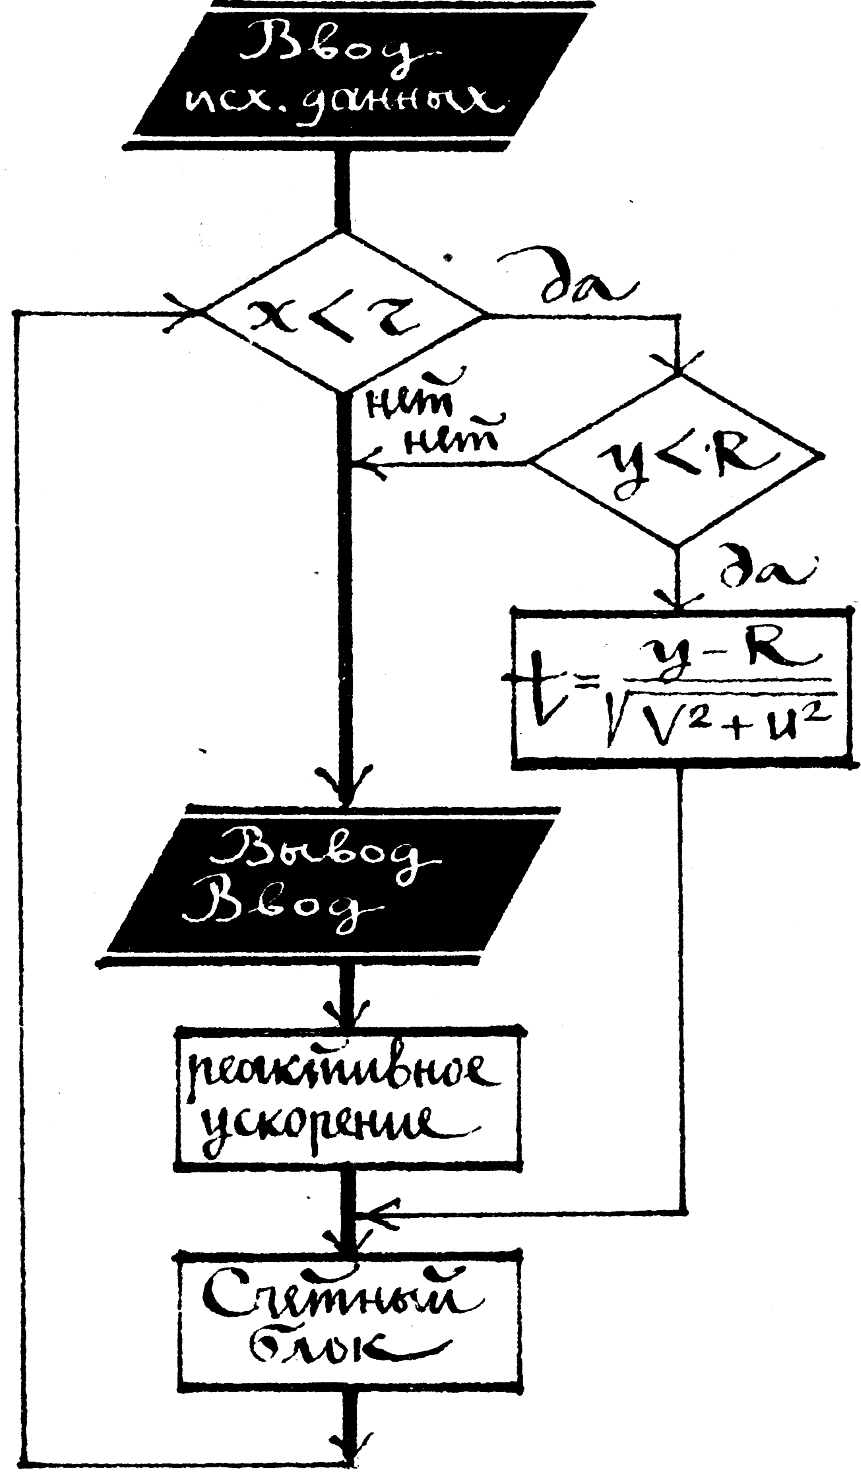
\includegraphics[width=0.5\textwidth]{jump_to_ug2}

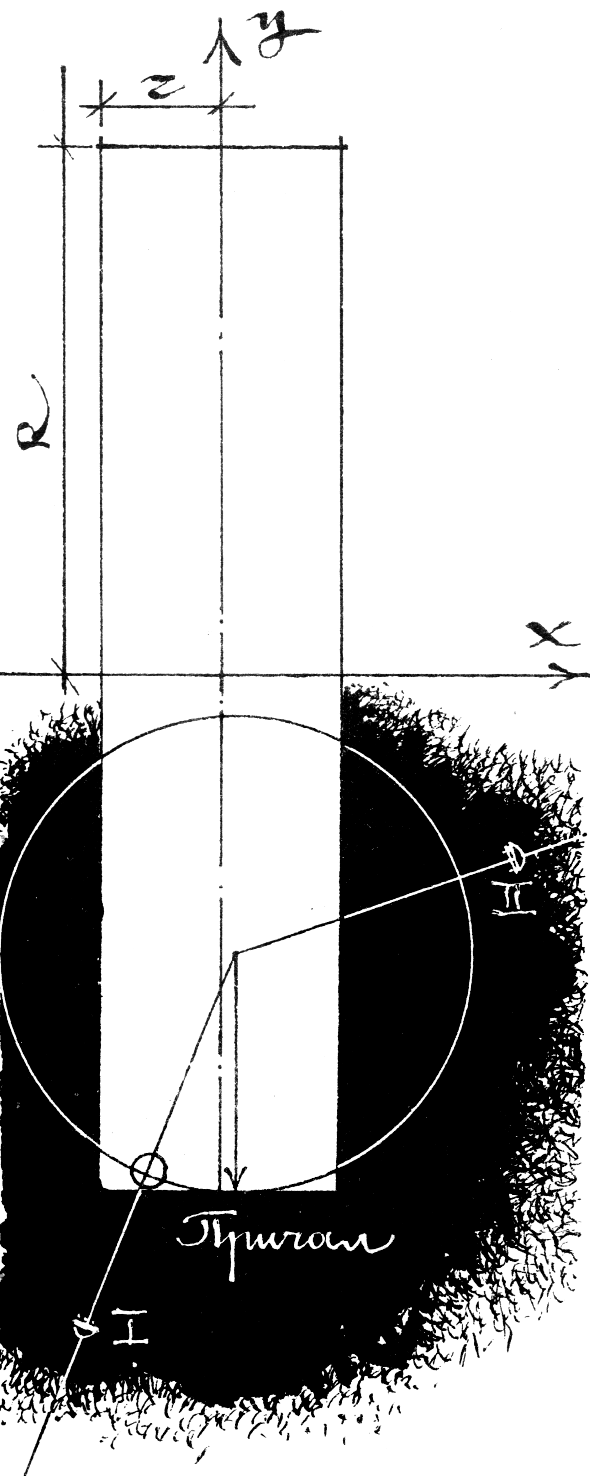
\includegraphics[width=0.5\textwidth]{jump_to_ug3}

Речь пойдет о путешествии не на юг, а на «ЮГ» — орбитальную станцию «Юрий Гагарин». Многие члены КЭИ с помощью программируемого микрокалькулятора и номеров нашего журнала смогли побывать на фантастическом спутнике Луны и не только любовались великолепным 600-метровым прыжком Лунного Коршуна, но и сами попробовали заняться космической «акробатикой». Однако сначала требовалось причалить к станции, а эта операция не менее сложна, чем посадка.

Поэтому сегодня мы рассмотрим блок-схему программы ОС-2, которая моделирует маневры космического аппарата в окрестности орбитальной станции цилиндрической формы, причем продольная ось станции совпадает с местной вертикалью, а посадочные площадки оборудованы на торцах цилиндра.

Тем, кто впервые занимается алгоритмической гимнастикой, советуем предварительно ознакомиться с предыдущими выпусками (см. «ТМ» № 5-7 за этот год). Ну а наши постоянные читатели легко разберутся в структуре программы.

Прежде всего мы видим блоки ввода-вывода. Их назначение понятно без комментариев. Затем следуют также знакомые по предыдущим выпускам вычислительные блоки, где определяется реактивное ускорение и подсчитываются значения текущих координат после каждого маневра. Напомним, что в нашей задаче система координат связана со станцией, причем ось Y направлена по местной вертикали, а ось X — вдоль касательной к траектории станции (см. рисунок). Так как посадочные площадки расположены на основаниях цилиндра, то условие причаливания имеет вид |у| = R, а |х|<r. (При этом, естественно, нельзя забывать о скорости в момент рандеву — ведь от нее зависит «мягкость» причаливания.)

Как и на прошлых занятиях, мы встречаемся также с блоками проверок и коррекции. Они-то и составляют «изюминку» игровых программ, поэтому, как обычно, их работу мы рассмотрим поподробнее. Обычно при последнем маневре не удается абсолютно точно провести стыковку. Чаще всего вычисленные значения координат лежат внутри станции. Авария? Нет, на индикаторе вы увидите вовсе не сигнал ошибки, наш бортовой компьютер скорректирует действия пилотов. Действует он при этом следующим образом: установив с помощью проверок значений координат, что лунолет «протаранил» станцию, калькулятор начинает извлекать его оттуда и превращается в своеобразную «машину времени». Вычисляется продолжительность «шага назад», и аппарат возвращается по своей траектории. Подобным же образом бортовой вычислитель действует и в других программах, но сегодня мы познакомимся с новым алгоритмом.

Случай первый — мы подлетели к станции с ее торца, но в результате последнего маневра аппарат очутился в «ЮГе». Что теперь делает ПМК?

Прежде всего он определяет расстояние до основания цилиндра, затем делит его на скорость аппарата в конечной точке и тем самым находит время «шага назад». Затем, как обычно, лунолет возвращается по прежней траектории. Геометрический смысл алгоритма показан на рисунке — точка, в которой оказался космический корабль, принимается за центр, и проводится окружность, радиус которой как раз равен расстоянию до торца. Пересечение окружности с траекторией — новое положение аппарата. Так за несколько шагов бортовой компьютер извлекает «Кон-Тики» на посадочную площадку.

Если же мы подлетели к станции сбоку, то применение того же самого способа коррекции дает совсем другой результат. Обратимся к рисунку. Легко видеть, что точка пересечения окружности с траекторией теперь лежит вне станции, корабль как бы отброшен назад от станции. Именно с этим эффектом «метеорной защиты» столкнулся героический экипаж «Кон-Тики». Надеемся, что нашим читателям при разработке собственных игр не составит труда смоделировать «силовое поле», столь любимое писателями-фантастами.

И несколько слов о блоке вычисления переменных. Отметим, что в нем использованы не точные, как в программе «Лунолет», решения уравнений движения, а приближенные.

Они получены с помощью так называемой линеаризации. О том, что это такое, мы поговорим в одном из ближайших выпусков рубрики.

Сергей ВОЛКОВ, инженер

\section{термодирижабль}
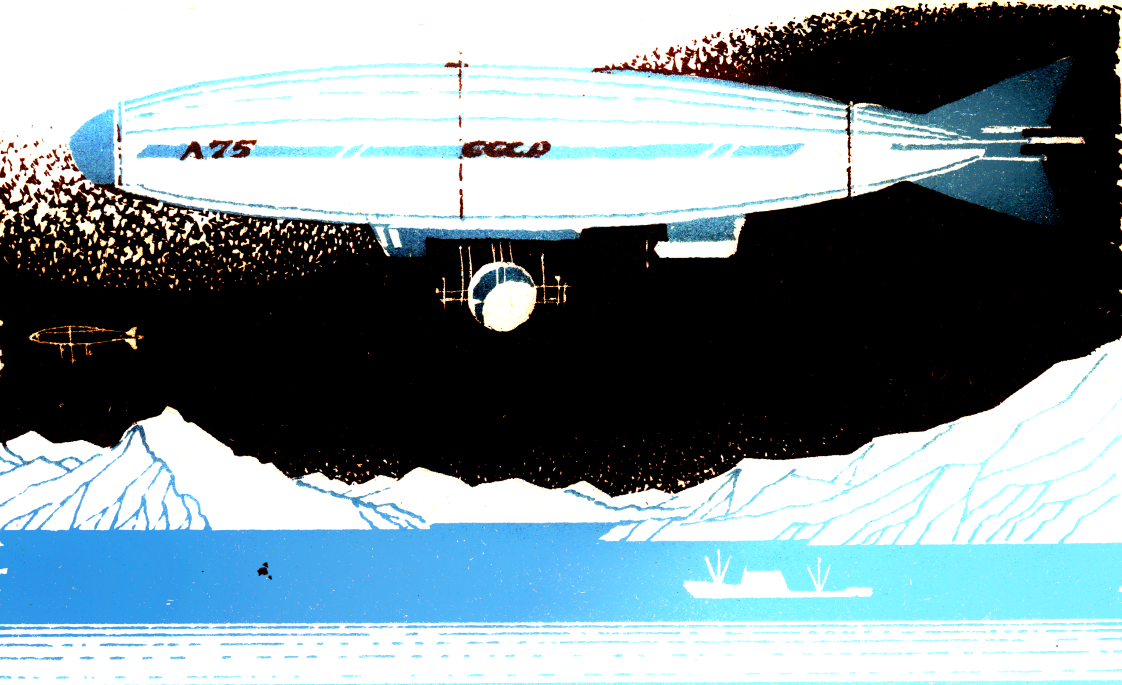
\includegraphics[width=\textwidth]{zeppelin}

Очень многие читатели в своих письмах высказывают единодушное пожелание: публиковать побольше игр, «хороших и разных». Идя навстречу этому пожеланию, предоставляем слово нашим постоянным авторам — Ю. Пшеннику из г. Молодечно Минской области и Г. Горовому из Керчи.

\begin{figure}[H]
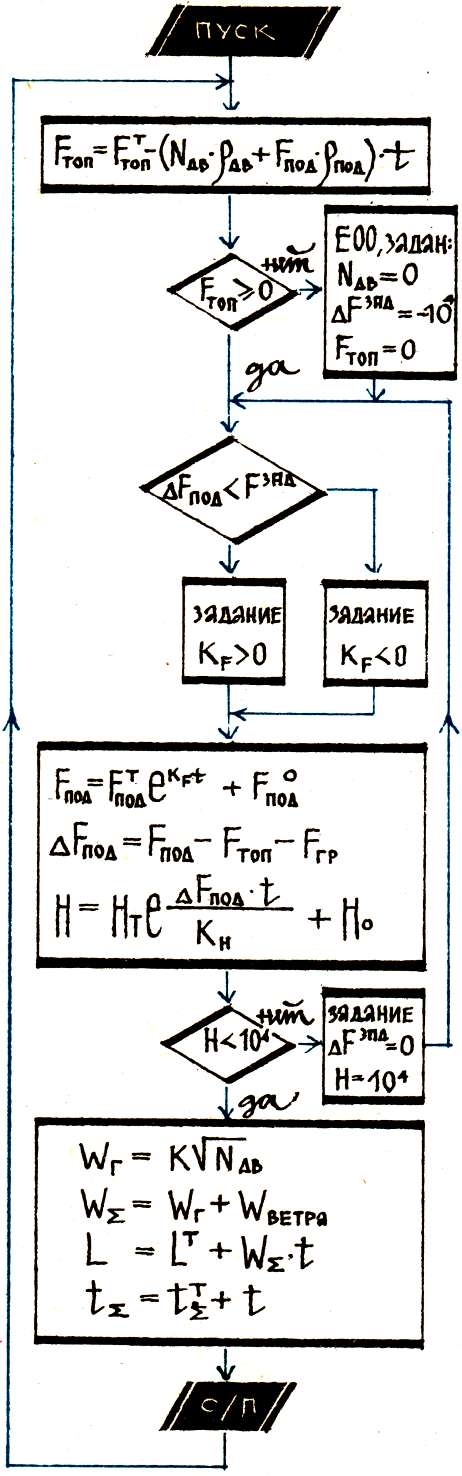
\includegraphics[width=0.5\textwidth]{zeppelin2}
\caption{Блок-схема программы «Термодирижабль». Условные обозначения: N$_{dv}$ — мощность двигателя; $\Delta$F$_{zad}$ —  заданное отличие подъемной силы от переменной составляющей веса; $\Delta$F$_{pod}$ — реальное отличие подъемной силы от переменной составляющей веса; F$_{gr}$ — вес груза; F$_{top}$ — вес топлива; Н — высота полета; W — скорость полета; W$_{wind}$ — скорость ветра; L — суммарная дальность полета; t — шаг по времени; t$_{\xi}$ — суммарное время полета.}
\end{figure}
00.ИП4 01.ИП0 02.5 03.$\div$ 04.ИП5 05.2 06.F10$^{x}$ 07.$\div$ 08.+ 09.ИП2 10.x 11.- 12.Fx$geq$0 13.72 14.П4 15.ИП6 16.ИП1 17.- 18.Fx<0 19.82 20.5 21.F1/x 22.ИП2 23.x 24.Fe$^{x}$ 25.ИП5 26.x 27.6 28.0 29.0 30.+ 31.П5 32.ИП3 33.- 34.ИП4 35.- 36.П6 37.ИПД 38.$\div$ 39.ИП2 40.x 41.Fe$^{x}$ 42.ИП7 43.x 44.2 45.+ 46.П7 47.ИПД 48.- 49.Fх<0 50.86 51.ИП0 52.F$\sqrt{}$ 53.5 54.x 55.ИП9 56.+ 57.П8 58.ИП2 59.x 60.ИПА 61.+ 62.ПА 63.ИПВ 64.ИП2 65.+ 66.ПВ 67.ИП8 68.ИП7 69.С/П 70.БП 71.00 72.0 73.П0 74.П4 75.ИПД 76./-/ 77.П1 78.ИПС 79.С/П 80.БП 81.15 82.5 83./-/ 84.БП 85.21 86.0 87.П1 88.ИПД 89.П7 90.БП
91.15

Программа моделирует полет на термодирижабле с учетом встречного (или попутного) ветра. Аппарат комбинированный — постоянная составляющая веса (конструкция, оболочка, оборудование) компенсируется гелиевыми баллонетами, переменная составляющая (полезный груз плюс топливо) — обогреваемым воздушным баллонетом. Изменением температуры внутри его регулируется подъемная сила (и соответственно высота полета). Горизонтальная скорость — за счет изменения мощности двигателя.

Задача — доставить груз в нужный пункт как можно быстрее, израсходовав при этом минимальное количество топлива. Перелет лучше всего осуществлять по карте по конкретному маршруту; если он проходит в горной местности, нужно следить, чтобы не врезаться в какую-нибудь вершину.

После ввода программы следует задать константы и начальные значения переменных. В регистр 0 вводится мощность двигателя в л.с. (рекомендуемые значения — от 0 до 1000); в регистр 1 — заданное отличие подъемной силы от переменной составляющей веса дирижабля в кг (от —10$^{4}$ до 10$^{4}$); в регистр 2 — шаг по времени в часах (от 0 до 3); 3 — вес груза в кг (от 0 до 10$^{4}$); 4 — вес топлива в кг (от 0 до 5000); 5 — подъемная сила в кг (ее начальное значение рекомендуется задавать равным ИП3 ИП4 + П5); 6 — реальное отличие подъемной силы от переменной составляющей веса (в начале — 0 П6, затем оно автоматически приближается к заданному в регистре 1); 7 — текущая высота полета в м; 8 — скорость полета в км/ч; 9 — скорость ветра в км/ч (от —100 до 100, минус соответствует встречному ветру); А—суммарная дальность полета (0 ПА) в км; В — суммарное время полета в часах (0 ПВ). В регистр С вводится сигнал об окончании топлива Е00 (100 К— ВП ПС), в регистр Д — постоянный коэффициент 1 ВП 4 ПД.

Для запуска программы надо отдать команду В/О С/П. При останове на индикаторе высвечивается текущая высота полета, в регистре Y — скорость, она вызывается на индикатор командой \XY. Остальные параметры можно посмотреть, вызвав их из соответствующих регистров. Примерное время счета 40 с. Повторный запуск программы клавишей С/П. (Если после очередного цикла какой-либо параметр требует коррекции, соответствующая величина вводится непосредственно в регистр; часто коррекция не требуется.)

Контрольный пример: 500 П0 5 ВП 3 П1 1 П2 1 ВП 4 П3 ПД 2 ВП 3 П4 + П5 1000 П7 10 /-/ П9 Сх П6 П8 ПА ПВ, регистр С заполнить согласно инструкции, В/О С/П. После останова на индикаторе высота 1417,78. \XY (101,8). Смотрим остальные переменные: ИП4 (1780) ИП5 (15256,8) ИП6 (3476,83) ИПА (101,8) ИПВ (1). Содержимое остальных регистров не изменилось, можно продолжать полет.

Варианты игровых ситуаций. Для взлета задаем положительное число в регистре 1. Воздушный баллонет дирижабля начинает прогреваться. Через несколько циклов, когда реальное отличие подъемной силы над весом станет заметным, высота полета начнет быстро увеличиваться — дирижабль отходит от причальной мачты. Теперь нужно задать величину скорости ветра и его направление, и можно включать двигатель.

При приближении к нужной высоте полета регистр 1 следует обнулить или сделать его содержимое слегка отрицательным. Постепенно происходит стабилизация высоты. По достижении «потолка» (10 000 м) она выполняется автоматически.

Для осуществления посадки в регистр 1 нужно ввести отрицательное число (порядка —1000 или еще меньше). При окончании топлива двигатель дирижабля автоматически отключается, и корабль дрейфует по ветру, постепенно снижаясь. Для ускорения посадки можно отдать команду 0 П5. При этом нагретый воздух в воздушном баллонете вытесняется наружным, и дирижабль идет на снижение.

Ю. ПШЕННИК

\section{МОРСКОЙ БОЙ}
Сегодня вашим партнером в этой увлекательной игре будет не человек, а ПМК «Электроника БЗ—34» (МК-54). Очевидно, вид кораблей и состав флотилии особого значения не имеют. Уточним правила:
\begin{enumerate}
\item игра ведется на поле размером 10Х10 клеточек;
\item кораблей восемь, каждый занимает отдельную клеточку;
\item информация выдается в виде: «попал» — «не попал»;
\item игровое поле нумеруется по вертикали и по горизонтали цифрами от нуля до девяти (см. рисунок);
\item координаты корабля задаются двузначным числом: первая цифра берется по вертикали, вторая — по горизонтали. Например, корабли на рисунке имеют координаты 05 (А), 10 (Б), 11 (В), 36 (Г), 42 (Д), 50 (Е), 61 (Ж), 79 (3). Ноль впереди опускается, поэтому координата корабля А-5, именно так его и представит ПМК.
\end{enumerate}

Теперь познакомимся с математической моделью игры. Необходимо, чтобы ПМК мог «обстреливать» все клетки игрового поля и при этом нигде не повторялся. Эта задача реализована с по- .мощью так называемого генератора псевдослучайных чисел (он пригодится и при других играх):

\begin{equation}
N_{i+i} =N_{i}*q—[N_{i}*q/P]*P,
\end{equation}

где квадратные скобки означают целую часть числа, Р — простое число, a q имеет вид $q=P—3^{m}$ и выбирается близким к Р/2. Если взять Р=101, q=74 (при m=3), то получим псевдослучайный ряд чисел на интервале (1,100). Вычитая из всех чисел по единице, получим ряд на интервале (0,99); он-то нам и нужен. Программа состоит из двух частей — программа распределения кораблей в памяти ПМК (часть А):

\begin{figure}[H]
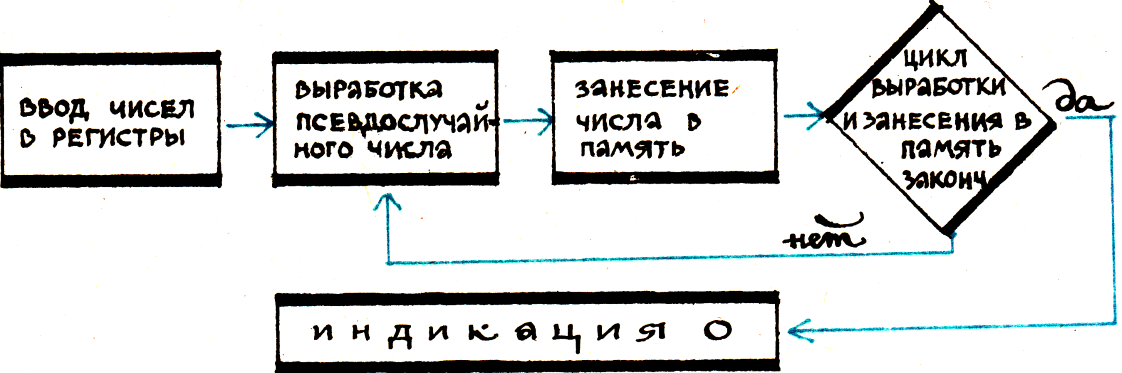
\includegraphics[width=\textwidth]{sea1}
\caption{Блок-схема программы распределения кораблей по игровому полю}
\end{figure}

00.ПВ 01.1 02.0 03.1 04.ПД 05.1 06.1 07.П0 08.8 09.П1 10.П2 11.ПП
12.34 13.КП0 14.FL1 15.11 16.Сх 17.С/П
34.ИПВ 35.7 36.4 37.x 38.ПС 39.ИПД 40.$\div$ 41.ПВ 42.КИПВ 43.ИПС 44.ИПВ 45.ИПД 46.x 47.- 48.ПВ 49.1 50.- 51.Fх<0 52.58 53.7 54.4 55.ПВ 56.7 57.3 58.В/0

и программа игры (часть Б):

\begin{figure}[H]
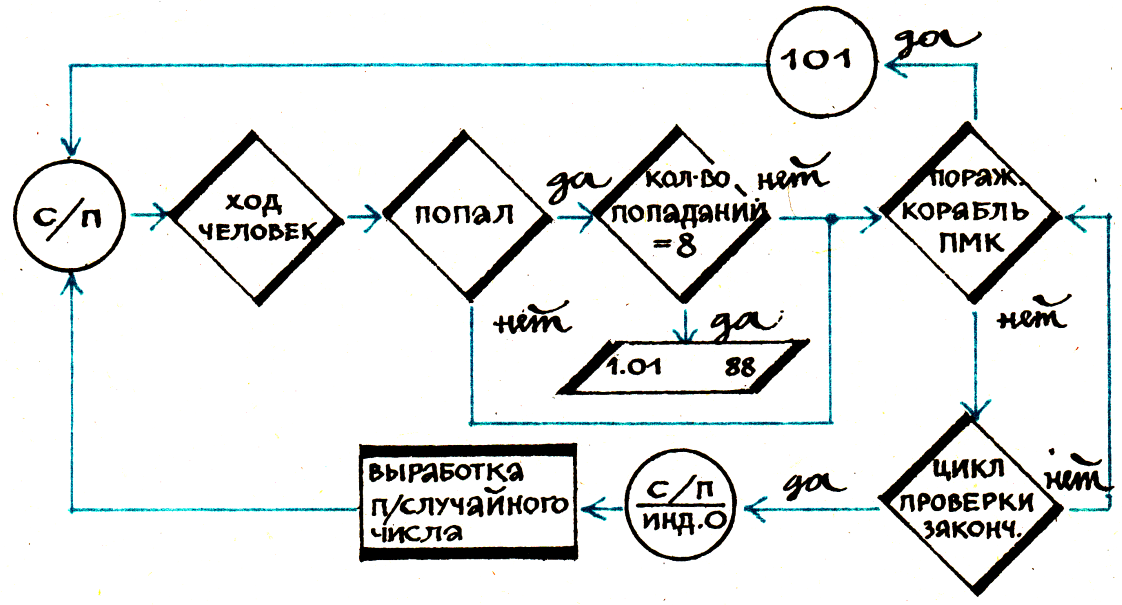
\includegraphics[width=\textwidth]{sea2}
\caption{Блок-схема игры морской бой}
\end{figure}

00.ИПД 01.С/П 02.ПС 03.ИПД 04.- 05.Fx$\neq$0 06.23 07.1 08.1 09.П0 10.8 11.П1 12.ИПС 13.КИП0 14.- 15.Fx$\neq$0
16.00 17.FL1 18.12 19.Сх 20.С/П 21.БП 22.34 23.КИП2 24.ИП2 25.Fх=0
26.34 27.ИПД 28.ВП 29.8 30.6 31.С/П 32.БП 33.31

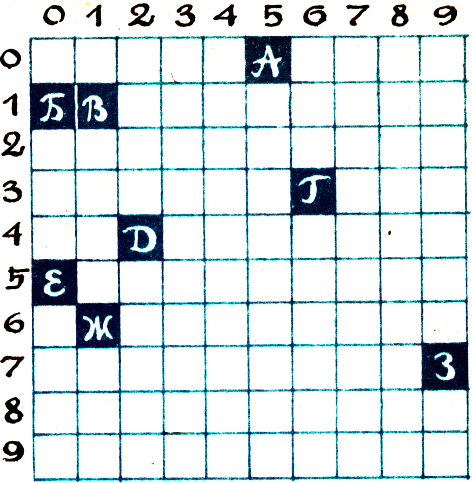
\includegraphics[width=0.5\textwidth]{sea3}

Рассмотрим часть А. Блок-схема алгоритма распределения кораблей представлена на рисунке. (При наборе программы адреса с 18-го по 33-й пропускаются.) После ввода программы нажать В/О, затем набрать любое целое положительное число (можно и 0) и С/П. Примерно через 65 с на индикаторе загорится 0 — корабли распределены по игровому полю. Контрольный пример: 123 В/О С/П. После останова корабли расставлены, как на нашем рисунке: ИПА (11) ИП9 (79) ИП8 (61) ИП7 (42) ИП6 (50) ИП5 (36) ИП4 (10) ИПЗ (5). После завершения расстановки кораблей надо нажать В/О и вводить часть Б. При этом она заполняет программную память на участке 00-33, а с адреса 34 остается та часть программы А, где реализуется выработка псевдослучайного числа. Если после перехода в режим АВТ нажать С/П, то первый ход сделает ПМК. Если же скомандовать В/О С/П, то на индикаторе загорится 101, и первый ход делает человек: нужно набрать координаты «выстрела» и нажать С/П. При попадании загорается 101, и ход следует повторить. Если промах — загорается ноль. Нажмите С/П — ход делает ПМК (высвечивает координаты клетки, по которой «стреляет»). Если он попал, сообщите об этом: ИПД С/П. ПМК повторит ход. При попадании в восьмой корабль машина высвечивает сигнал о победе (слева 1,01, справа 88) и самоблокируется — игра закончена. Для повтора игры придется ввести программы А и Б заново (фрагмент 34-58, естественно, можно не вводить). На выработку своего хода ПМК затрачивает не более 8-9 с, на проверку координат противника — не более 18 с.

Г. ГОРОВОЙ

\section{В ГЛУБИНАХ «ЭЛЕКТРОННОГО ОКЕАНА»}
В сообщении Д. Кайкова, опубликованном в № 7, рассказывалось о получении числа 01, на основе которого можно сформировать «разные другие коды». Независимо от него интересные изыскания по новым видеосообщениям провели В. Паникаровских из Перми, В. Вовк из города Барвенково Харьковской области, В. Мититель из Владимира, С. Пухов и С. Банников из Москвы, С. Ишутин из Свердловска. Расскажем о некоторых результатах, полученных в ходе небывалого «мозгового штурма».

Прежде всего образуем «пустышку» и зашлем ее в регистр Д: Сх К— ВП ПД, после чего для полной очистки стека нужно несколько раз подряд нажать стрелку вверх. На индикаторе 0. Нажмем 1 и применим к этой цифре алгоритм Д. Кайкова (см. № 7): ВП /—/ 1 ПС ИПД ИПС 1 ПС ПС стрелка вверх (три раза) ВП /—/ 30 и запишем результат, допустим, в регистр 7:П7. На индикаторе 01, это сообщение нам уже знакомо. На самом первом (нулевом) знакоместе воцарился 0. Нажмем /—/, подействуем на получившееся число (L1) тем же алгоритмом (ВП /—/ 1 и т. д.) и запишем результат (С1) в регистр 8. Новое применение того же алгоритма дает число Г1, запишем его в регистр 9. Наконец, вызовем из регистра 7 первое из полученных чисел (01), подействуем на него тем же алгоритмом и результат (на вид это обычная единица) запишем в регистр Д — «пустышка» больше нам не понадобится.

В регистрах 7, 8, 9 и Д находятся сейчас числа 01, С1, Г1 и 1. Их свойства необычны. Если нажать /—/, они преобразуются в L1, 1, Е1 и —1. Повторное нажатие /—/ возвращает числам первоначальный вид. Оператор ВП 1 КНОП обеспечивает отход десятичной точки от любого из этих сообщений (в том числе и от«псевдоединицы» из регистра Д). Оператор К— ВП КНОП заменяет 1 во всех этих сообщениях на букву Е. А чтобы заменить единицу каким-либо другим символом, нужно предварительно ввести в ПМК программу: 00.\XY 01.КНОП 02.ВП 03.С/П, затем в режиме АВТ получить на индикаторе нужный символ, вызвать из регистра преобразуемое сообщение и нажать В/О С/П. Полученный таким образом шифр сохраняет все свойства исходного.

Наиболее интересна для формирования новых видеосообщений «псевдоединица», находящаяся сейчас в регистре Д. Скомандуем ИПД ВП, допустим, 4 П1, затем КИП1 (пять раз) ИП1 ВП /—/ 4 КНОП. В результате получилось видеосообщение (единица и отстоящий от нее на некоторое расстояние минус) типа тех, которые пригодились в перелете Луна — Земля. Варьируя цифру после ВП, этот минус можно поместить в произвольном месте индикатора (в пределах мантиссы). Единицу же слева с помощью процедур из предыдущего абзаца легко заменить на любой другой символ.

Еще одно полезное сообщение получается при ИПД К— ВП 1 F10$^{x}$ ВП /—/ 40 КНОП. Минус получен в порядке, на предпоследнем месте. Теперь, учитывая сообщения, использованные в «Пути к Земле», появилась возможность получать его в произвольной точке индикатора.

Очень интересную систему графических изображений на базе числа 0Е разработал учащийся Владимирского авиамеханического техникума Виктор Мититель. Сначала нужно занести это число в регистр 0. Для его получения скомандуем ИП7 (в регистре 7 у нас сейчас 01) К— ВП П0. Затем введем в ПМК короткую вспомогательную программу: 00.FL1 01.02 02.FL2 03.00 04.С/П 05.П3 06.ВП 07.С/П. Затем, перейдя в режим АВТ и прочистив стек (нажав Сх и несколько раз стрелку вверх), проделаем следующие манипуляции: ИП0 БП 05 С/П Fx$^{2}$ Fx$^{2}$ ВП 3 ВП \XY Сх \XY /—/ БП 05 С/П /—/ П4 (первое изображение изготовлено и заслано в регистр 4: ноль с минусом слева — это Земля и космическая станция, ноль справа — Луна). Далее: ВП /—/ 50 П5 (возле Луны появился космический корабль). Теперь нужно опять прочистить стек (рекомендуется делать это перед получением каждого нового изображения) и продолжать: 4 П2 Сх ИП0 П1 Сх В/О С/П ИП1 Fx$^{2}$ Fx$^{2}$ ВП 3 ВП \XY Cx \XY /—/ БП 05 С/П /—/ ВП /—/ 57 П6 (в кадре появилась еще и станция «Лагранж»).

Для получения шести последующих однотипных изображений нужно предварительно записать в регистр 0 число 0—: ИП0 /—/ БП 05 С/П /—/ П0. Теперь прочистить стек и формировать остальные кадры. ИП0 ВП 1 (для каждого последующего изображения порядок нужно увеличить на единицу; не забывайте предварительно прочищать стек) П1 Сх 5 П2 Сх В/О С/П ИП1 Fx$^{2}$ Fx$^{2}$ ВП 3 ВП \XY Сх \XY /—/ БП 05 С/П /—/ ВП /—/ 57 П7 (последующие кадры нужно, естественно, записывать в другие регистры, например, 8, 9, А, В, С). Последовательно выводя эти кадры на индикатор (скажем, проходя по совету В. Ивинских из Тольятти командой ПП по программе 00. ИП4 01.ИП5 02.ИП6 03.ИП7 04.ИП8 05.ИП9 06.ИПА 07.ИПВ 08.ИПС 09.ИП4 10.В/О), увидим воочию важнейшие этапы перелета Луна — Земля. Использованные приемы позволяют получить и многие другие интересные видеосообщения. Например, если в конце приведенных последовательностей вместо ВП /—/ 57 отдавать команду ВП /—/ 7, черточка окололунной станции на всех картинках исчезнет.

То ли еще будет! Как правильно пишет наш постоянный корреспондент В. Паникаровских, «электронный лабиринт, полный тупиков, бездонных провалов, узких боковых ходов и т. д., всегда под рукой у каждого поклонника Клуба электронных игр».

Ясное дело, имеется в виду наш любимый программируемый микрокалькулятор.

Михаил ПУХОВ

\section{ПРОИГРАВШИЙ ВЫИГРЫВАЕТ}
Мог ли французский математик Баше де Мезирьяк в 1612 году предполагать, какие последствия вызовет в XX веке его изобретение? Ничего не поделаешь, мы сами часто «не ведаем, что творим». Так что же «натворил» Баше? Он придумал игру (ныне она носит его имя). Правила ее очень просты — первый игрок выбирает число от 1 до 10, второй прибавляет к нему любое число из того же интервала и т. д. Побеждает тот, кто получит в сумме 100.

По непонятным причинам (может быть, из-за трудностей с устным счетом?) со временем игра видоизменилась. Один из ее вариантов теперь выглядит так: из кучи, содержащей N мелких предметов (камешков, пуговиц, спичек и т. п.), играющие поочередно берут не менее одной и не более К штук. Выигрывает тот, кто сумеет взять последний предмет.

Коротать время за игрой Баше не очень-то интересно. Дело в том, что ее исход ясен еще до первого хода (конечно, если партнеры не делают ошибок). Невольно вспоминается анекдотическая история о «профессионалах-доминошниках», которые, раздав кости, сразу же их открывают и тут же записывают очки проигравших.

Победный алгоритм игры Баше легко получить, если рассуждать с «конца», то есть рассмотреть сначала позицию перед последним ходом. В самом деле, для выигрыша надо оставить противнику перед его последним ходом К+1 предмет. Тогда, сколько бы он ни взял (напоминаем, что больше К брать нельзя), своим ходом вы забираете последний. Поэтому, перед предпоследним ходом надо оставить на столе 2 (К+1) предметов. В этом случае, при любом ходе противника можно ответить так, что в куче останется К + 1 предмет, что и требуется. Таким образом, в игре есть ряд позиций — их называют особыми — К+1, 2(К+1), 3(К+1) предметов и т. д., когда начинающий проигрывает. Значит, если начальная позиция неособая, то нужно сразу же получить особую позицию, взяв «лишние» предметы, и затем уверенно доводить игру до победы. Если же в особой позиции ваш ход, остается лишь уповать на то, что противник не читал этот номер журнала (или другой литературы, где описана стратегия игры Баше), и ждать его ошибки. Кстати, и в первоначальном варианте игры, естественно, также есть выигрышные позиции. Их указал сам Баше де Мезирьяк — 9, 19, 29 ...89.

Теперь перейдем к «эху XX века». При всей своей простоте, а может быть, именно по этой причине игра Баше стала для любителей математических развлечений «вечной темой», чем-то вроде классического «любовного треугольника» в литературе. С появлением же счетно-решающих устройств и вычислительных машин интерес к ней еще более возрос. Стали разрабатываться релейные схемы, программы для ЭВМ, позволяющие человеку сразиться с машиной. Более того, ввиду несложности выигрышного алгоритма порой удавалось построить «железного партнера» на необычной «элементной базе». По крайней мере, автору уже доводилось писать о созданной студентами Московского физико-технического института самообучающейся (!) машине из... спичечных коробков.

Естественно, владельцы программируемых микрокалькуляторов не могли пройти мимо возможности проверить свои силы в «битвах» с электронным противником. И редакции научно-популярных журналов, в том числе и «ТМ», захлестнул поток писем с программами для игры Баше. Администрация КЭИ оказалась в затруднительном положении, чью программу публиковать — инженера из города Тореза Донецкой области Игоря Лагуты, студента из Таганрога В. Бондаренко или свердловского семиклассника Дмитрия Сажина? А ведь еще прислали программы Н. Васильев из Горловки, А. Кадулин из Ростова-на-Дону, П. Ляховский из Херсона и многие другие читатели. Разобравшись в груде писем, мы довольно быстро с помощью ПМК установили, что если в каждом номере публиковать только по одной программе для игры Баше, то по крайней мере на ближайшие пять лет КЭИ обеспечен материалами. Но кому же интересно пять лет подряд читать про одно и то же, и поэтому администрация решила вообще не печатать программ игры Баше и аналогичных игр (ним, цзяньшидзы и т. п.).

Тем не менее мы настоятельно рекомендуем игру Баше для домашних упражнений, особенно начинающим самостоятельно писать игровые программы. Пусть она станет для вас своеобразными «прописями», на которых будет отрабатываться «программистский почерк». И когда ПМК станет уверенно вас обыгрывать, вы ощутите настоящую радость победы.

Сергей ВОЛКОВ, инженер

\section{ТО ВЗЛЕТ, ТО ПОСАДКА...}
Научно-технический прогресс оказывает воздействие и на художественную литературу. По крайней мере, Джеймсу Олдриджу в «Последнем дюйме» удалось добавить к «вечным» литературным сюжетам (а их число, как утверждают специалисты, весьма ограничено) еще один:' совершенно неподготовленный человек, руководствуясь указаниями другого, более опытного, благополучно производит посадку самолета. Нет нужды перечислять литературные произведения, а также кинофильмы, в основу которых положена аналогичная ситуация. Пошел по этому пути и наш автор В. Н. Лозовой. Но в отличие от своих предшественников он прислал в редакцию, помимо рассказа «Почти невероятный случай» (кульминационный момент которого мы воспроизводим), игровую программу «Самолет», позволяющую читателям в полной мере сопереживать герою рассказа.

Владимир ЛОЗОВОЙ, г. Армавир

\subsubsection{почти НЕВЕРОЯТНЫЙ СЛУЧАЙ}
Неподвижная ранее «клетчатая» поверхность земли с группами красноверхих домов-коробочек, букашками автомобилей и проблесками водной глади оживала и все быстрее устремлялась навстречу, проваливаясь куда-то назад, за каркас боковых стекол фонаря кабины пилотов. Бескрайняя синь, заливавшая остекление, уступала место живым и теплым краскам земли.

Двухсоттонный «боинг», ведомый автоматикой, снижался, словно кто-то тянул его за нос к международному аэропорту имени Шарля де Голля. Впереди, чуть не задевая колени, мелкими движениями отрабатывала колонка управления, слегка покачивая рогатым штурвалом. Справа, перед пустым креслом второго пилота, все эти движения повторялись другой колонкой. Казалось, я не нужен здесь, в этой на первый взгляд тесной кабине. Но это не так. Пройдет еще несколько минут, и мои руки лягут на шершавую кожу рукояток, взяв вместе со штурвалом мою собственную судьбу и судьбу еще трехсот человек. Никто из них не знал — а может, никогда не узнает,— что самое важное в их жизни событие впереди.

К действительности меня вернул голос в наушниках:

— Аэропорт Шарль де Голль к аварийному «боингу». Как дела на борту?

— Техника вроде в порядке, пассажиры ничего не подозревают, командир и второй пилот без сознания в салоне первого класса. Как мои дела с земли?

— Идешь отлично, через Пятнадцать минут будешь в заданной точке. Слушай, парень, дальше тебя будет вести шеф-пилот фирмы «Боинг», передаю ему связь.

— хорошо, жду.

— Хэлло, парень, как тебя зовут?

— Дик, Дик Чизмен, зовите просто Дик.

— Хорошо, Дик, называй меня Мэтом, договорились?

— Договорились, Мэт.

Последовала небольшая пауза.

— Дик, посмотри высоту и скорость.

— Высота 600 м, скорость 520 км/ч.

— Видишь — справа от тебя желтая рукоятка выпуска шасси?

— Нашел.

— Надави на красный флажок и назад до упора.

— Есть.

— Смотри на транспарант перед рукояткой, на нем должна загореться надпись «Шасси выпущено».

В недрах фюзеляжа послышалось еле слышное протяжное урчаний, затем легкий толчок — стойки стали на замки.

— Есть.

— Молодец, сынок, дай скорость и высоту.

— Скорость 480 км/ч, высота 300 м.

— Отлично, справа в центре сектора газа — четыре сцепленные рукоятки. Переведи их в положение 0,2 номинала.

— Есть.

— Теперь следи за скоростью. Когда упадет до 350 км/ч, выпустишь закрылки и предкрылки. Посмотри на левую панель, видишь красный кожух с надписью «закрылки»? Откинь его; там кнопки, видишь?

— Да, Мэт.

— При скорости 350 нажмешь под надписью «30 градусов». Понял? Доложишь по исполнении.

Самолет терял скорость. Чтобы не терять высоту, автопилот поднимал его нос в небо.

— Мэт, скорость 350, высота 300, выпускаю закрылки.

— Хорошо, малыш.

— Закрылки вышли, загорелся транспарант!

— Отлично, Дик, дай высоту и скорость.

— Высота 300, скорость 350,

— Отлично, у тебя над головой панель автопилота. Возьми левой рукой штурвал, а правой выключи тумблер канала тангажа, видишь надпись? Будь готов к легкому рывку на штурвале и потом держи высоту, контролируя вертикальную скорость по вариометру, понял?

— Ясно.

— Следи за путевой скоростью, держи 300 км/ч.— Мэт помолчал немного и добавил:—Смотри перед собой, полосу видишь? Сейчас начнем посадку. Внимание, Дик, поставь рукоятку управления двигателями на малый газ.

— Сделал, Мэт.

— Теперь, сынок, гаси скорость до 270, но снижаться ниже двухсот метров упаси тебя бог. До полосы осталось 18,7 км.

Особых эмоций я не испытывал. Работа полностью захватила меня. Передо мной стояла задача, и я должен был ее выполнить. Знакомое по восхождениям чувство полной собранности и ответственности за каждое движение вытеснило из души все страхи и сомнения. На другом конце моей веревки в связке со мной сейчас были триста человек. Я не имел права на отступление или ошибку. Тем более что вряд ли мне удастся уйти на второй круг и вновь зайти на посадку. Это нужно было сделать с первого захода.

Руки держали штурвал, взгляд последовательно обегал вариометр, высотомер, авиагоризонт и указатель скорости. Автопилот держал курс и крен. Изредка я бросал взгляд вперед, где уже совсем рядом мчалась земля, набегая далекой еще бетонкой.

Скорость медленно падала, я же медленно выбирал штурвал на себя, ориентируясь по вариометру. Прошло пятьдесят секунд спуска.

— Мэт, вертикальная скорость снижения 1,6 м/с, скорость 291 км/ч.

— Энергичней штурвал на себя. Все нормально.

Я чуть взял штурвал на себя, и скорость снижения сразу стала падать. 0,7 м/с, 0,14 м/с, 0,1 м/с... Не слишком ли? Стоило так подумать, как руки сами отреагировали замедлением и скорость снижения прыгнула до 0,7 м/с (внимание автоматически отметило: 100 с снижения, высота 257 м). Двигателей почти не было слышно, лишь плотные потоки воздуха свистели за бортом.

«Ого, да за этими руками нужно еще и следить!» — мелькнуло в сознании, я сразу заставил их вытянуть штурвал еще немного на себя, и самолет стал медленно уменьшать скорость снижения.

— Мэт, высота 236, скорость 274 км/ч, иду с набором 0,02 м/с.

— Слушай, Дик, продолжай снижать скорость до 270, энергичней иди вниз, держи скорость снижения 2-3 м/с. Хорошо идешь, парень!

Я остановил штурвал и стал следить, как растет скорость по вариометру. 0,9 м/с, 2,2 м/с — пора подтягивать, пока не перескочил за 3 м/с. Эту многотонную махину разгонять было страшно. Внизу только 176 м, а что это для двухсоттонной громадины?

— Мэт, скорость 270, скорость снижения 2,9 м/с.

— Выводи двигатели на 0,65 номинала.

Правая рука легла на сектора газа, и глаза проконтролировали отметку 0,65. Свист турбин усилился, затем перешел в ровный вой. Через 20 с тяга была заданной.

— Высота 116, скорость снижения 3 м/с, скорость 271 км/ч.

— Хорошо, малыш, так держать. Будь готов убирать газ.

Земля была рядом, стало не до радиообмена. Через пятнадцать секунд высота упала до 23 м — пора начинать выравнивание. Еще чуть ручку на себя и сбросить тягу, а то пошел разгон.

Еще пять секунд. Высота 11 м, снижение 2,2 м/с. Четыре секунды — высота 5,5 м, снижение 1,5 м/с. Еще три секунды— высота 3 м, снижение 1 м/с, скорость 271 км/ч. Продолжаю удерживать штурвал и перевожу двигатели на малый газ. Прошло еще девять секунд, и колеса мягко коснулись нагретого солнцем бетона.

В наушниках грянул гром. Сквозь этот шум выкриков, рукоплесканий, поздравлений вдруг прорвался и все подавил собой чуть с хрипотцой голос Мэта:

— Теперь только держи педалями ось полосы, держи ось и не забывай про тормоза, парень!

* * *

Я убежден: почти каждый настоящий любитель техники признает за самолетами высшее техническое совершенство, конструктивную да и просто эстетическую красоту. Но гораздо меньшая часть читателей «ТМ» знакома с тем трудом, который необходим для уверенного управления воздушным гигантом.

К счастью, возможности «Электроники БЗ-34» позволяют довольно точно моделировать полет самолета. Вот соответствующая программа:

\begin{figure}[H]
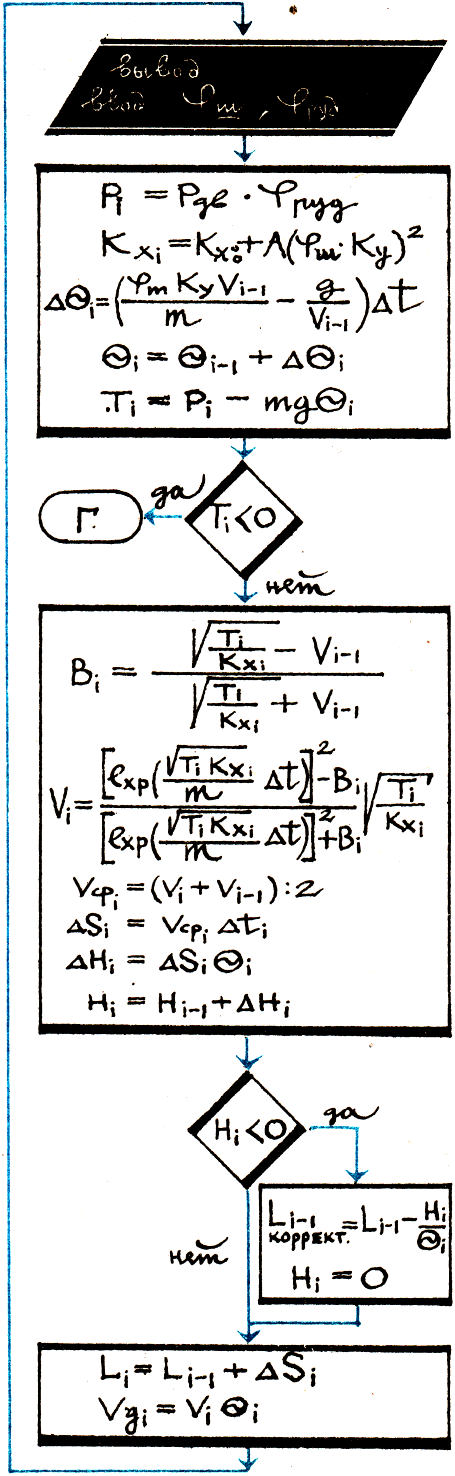
\includegraphics[width=0.25\textwidth]{airplane}
\caption{Блок-схема программы «Самолет».}
\end{figure}
00.ИП6 01.x 02.\XY 03.ИП2 04.x 05.$\uparrow$ 06.Fx$^{2}$ 07.ИП3 08.x 09.ИП1 10.+ 11.П7 12.\FO 13.ИП0 14.х 15.ИП5 16.$\div$ 17.ИП4 18.ИП0 19.$\div$ 20.- 21.ИПД 22.x 23.ИПВ 24.+ 25.ПВ 26.ИП4 27.х 28.ИП5 29.x 30.- 31.Fx<0 32.35 33.ИП9 34.с/п 35.ИП7 36.$\div$ 37.F$\sqrt{}$ 38.П8 39.ИП0 40.ПП 41.88 42.ИП7 43.x 44.ИПД 45.х 46.ИП5 47.$\div$ 48.Fe$^{x}$ 49.Fx$^{2}$ 50.\XY 51.ПП 52.88
53.x 54.ИП0 55.\XY 56.П0 57.+ 58.2 59.$\div$
60.ИПД 61.х 62.П7 63.ИПВ 64.х 65.ИПА 66.+ 67 Fx<0 68.76 69.ИПВ 70.$\div$ 71.ИПС 72.\XY 73.- 74.ПС 75.0 76.ПА 77.ИПС 78.ИП7 79.+ 80.ПС 81.ИП0 82.ИПВ 83.x 84.ИПА 85.с/п 86.БП 87.00 88.- 89.$\uparrow$ 90.FBx 91.2 92.x 93.+
94.$\div$ 95.ИП8 96.в/о

После ее ввода в регистры памяти для моделирования посадки самолета-гиганта «Боинг-747» необходимо записать следующие величины: начальная скорость полета V=83,33 м/с в регистр 0; коэффициент сопротивления самолета К$_{xo}$=55,2 в регистр 1; коэффициент подъемной силы Kq=521 в регистр 2; коэффициент индуктивного сопротивления А= 0,000222 в регистр 3; ускорение свободного падения g=9,81 м/с$^{2}$ в регистр 4; посадочная масса т = =204000 кг в регистр 5; номинальная тяга двигателей P$_{dv}$=848565 Н в регистр 6; начальная высота полета Н=300 м в регистр А; угол наклона траектории в радианах $\Theta$=0 в регистр В; координата начальной точки на поверхности земли L=0 в регистр С; временной шаг программы $\Delta$t (в секундах) в регистр Д. В регистр 9 вводится аварийный сигнал (например,- буква Е: 1 К— ВП П9).

В начальный момент самолет с выпущенным шасси и механизацией крыла в посадочной конфигурации находится на высоте 300 м и летит горизонтально со скоростью 300 км/ч (примерно 83,33 м/с). Согласно тексту до передней кромки ВПП осталось 18,7 км. Ваша задача — управляя секторами газа и штурвальной колонкой, достигнуть поверхности полосы (Н=0) на расстоянии не более 100 м от ее передней кромки (ИПС= 18800). При этом скорость снижения не должна превышать 3 м/с. Путевая скорость в момент касания полосы не должна превосходить 300 км/ч.

Управляющими параметрами являются положение рукоятки управления двигателями (РУД) и Штурвала. Полная тяга соответствует $\varphi_{rud}$ = 1, «малый газ» — $\varphi_{rud}$ = 0,04. Максимальная подъемная сила обеспечивается при выборе штурвала «на себя». Диапазон его отклонений определяется от $\varphi_{sh}$=1 («штурвал на себя») до $\varphi_{sh}$ = —1 («штурвал от себя»).

Траектория, по которой самолет подходит к ВПП, называется глиссадой. Ее оптимальные параметры для пассажирских и учебного самолетов указаны в таблице. Непосредственно перед приземлением необходимо с высоты не менее 10 м произвести выравнивание 
и уменьшить скорость снижения до 1-2 м/с в момент касания полосы.

Начиная игру, следуют установить переключатель Р—Г в положение Р (радианы), затем набрать величину выбранного отклонения штурвала, нажать стрелку вверх, набрать величину отклонения РУД, затем С/П (при первом ходе В/О С/П). В среднем через 38-40 с программа закончит счет: на индикаторе горит текущее значение высоты в м. В регистре У находится скорость снижения в м/с, она вызывается на индикатор командой \XY. Остальные переменные хранятся в прежних регистрах.

Загорание на индикаторе нуля означает соприкосновение самолета с поверхностью земли. Если при этом скорость снижения лежит в диапазоне 3—6 м/с, вы потерпели аварию; если же скорость еще больше, то это верная катастрофа. Если вы приземлились на бетон более чем на 100 м от передней кромки ВПП, то самолет выкатится за пределы полосы и авария опять-таки неизбежна. Приземление до кромки ВПП — как правило, катастрофа. Наконец, если скорость при посадке превышает 300 км/ч, то вы также терпите аварию, выкатываясь за пределы бетонки.

Появление аварийного сигнала (буква Е) на индикаторе означает, что самолет начал набирать высоту с недопустимым для установленной тяги двигателей углом. Он резко теряет скорость и рискует сорваться в штопор, этот режим полета — аварийный. Можно считать, что пилоту с квалификацией Дика Чизмена выбраться из такой ситуации не удастся. Рекомендую при ответственных маневрах уменьшать шаг по времени (число в регистре Д), памятуя, что реакция нетренированного человека составляет 0,5—1 с, в зависимости от сложности ситуации.

Вторым по сложности (после посадки) маневром для гражданского самолета является взлет. Для его выполнения необходимо ввести в качестве начальной скорость отрыва и ввести в регистры памяти ПМК взлетные характеристики самолета. Следует иметь в виду, что заложенная в программу математическая модель достаточно точно описывает движение самолета только при углах наклона траектории, не превышающих по абсолютной величине 15\degree.

Ну а теперь садитесь на место Дика Чизмена и попытайтесь повторить его невероятную, прямо-таки фантастическую удачу...

ИСХОДНЫЕ ДАННЫЕ
ДЛЯ ПОСАДКИ И ВЗЛЕТА
НЕКОТОРЫХ ТИПОВ САМОЛЕТОВ

\begin{table}[H]
\begin{tabular}{|l|l|l|l|l|l|l|}\hline
\multirow{2}{*}{№ регистра} & \multicolumn{2}{l}{Лайнер} & \multicolumn{2}{l}{Аэробус} & \multicolumn{2}{l}{Учебный} \\
                            & посадка     & взлет        & посадка      & взлет        & посадка       & взлет       \\\hline
0                           & 69          & 78,5         & 83,33        & 83,33        & 47,3          & 33          \\\hline
1                           & 21,2        & 13,9         & 55,2         & 32           & 0,51          & 0,364       \\\hline
2                           & 174         & 174          & 521          & 521          & 18,2          & 15,8        \\\hline
3                           & 0,00024     & 0,000283     & 0,000222     & 0,000201     & 0,0095        & 0,0048      \\\hline
5                           & 65000       & 84000        & 204000       & 352000       & 1470          & 1500        \\\hline
6                           & 295000      & 295000       & 848565       & 848565       & 3741          & 3741        \\\hline
А                           & 400         & 0            & 300          & 0            & 150           & 0           \\\hline
В                           & 0           & 0            & 0            & 0            & 0             & 0          \\\hline
\end{tabular}
\end{table}

ОПТИМАЛЬНЫЕ ХАРАКТЕРИСТИКИ
ВЫПОЛНЕНИЯ МАНЕВРА

\begin{table}[H]
\begin{tabular}{|l|l|l|l|l|l|l|}\hline
\makecell{вертикальная скорость, м/с} & -3,3 & 1,6  & -3,3  & 1,9  & -2,2 & 7,6  \\\hline
\makecell{угол наклона траектории}    & -3\degree  & 1,1\degree & -2,5\degree & 1,2\degree & -3\degree  & 9,8\degree \\\hline
\makecell{путевая скорость, км/ч}     & 230  & 300  & 270   & 324  & 150  & 160  \\\hline
\makecell{конечная скорость, км/ч}    & 210  & 300  & 270   & 324  & 130  & 170  \\\hline
\makecell{дистанция маневра, км}   & 7,63 & 6,25 & 6,87  & 5,73 & 2,86 & 0,69\\\hline
\end{tabular}
\end{table}

\section{ТРЕБУЕТСЯ ВЫИГРЫШНАЯ СТРАТЕГИЯ}

«Мы очень хотели бы увидеть на страницах журнала программы, реализующие игры с самим микрокалькулятором, то есть такие игры, в которых ПМК являлся бы игроком — соперником человека»,— пишут, выражая пожелания многих, семиклассники К. Трихин и Д. Белянов из города Бугры Ленинградской области. Одна из подобных игр — «Волки и козлик» Д. Кайкова — была опубликована в № 8. Это пример стратегической игры, от изобретательности программиста зависит здесь качество работы машины.

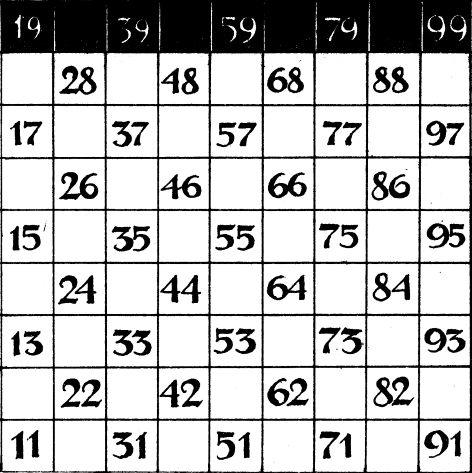
\includegraphics[width=0.25\textwidth]{win_strategy}

Напомним, что в игре Д. Кайкова использовалась обычная шахматная доска размером 8X8. Уйти от трех шашек на таком поле несложно, от четырех — невозможно. Значительно интереснее могут стать баталии шашки, ведомой ПМК, с четырьмя фишками противника на доске размером 9X9, изображенной на нашем рисунке. В начальной позиции шашки человека стоят на полях 19, 39, 79 и 99, шашка электронного «гроссмейстера» — в центре доски, на клетке 55. Первый ход, как и в программе Кайкова, делает ПМК. Легко видеть, что при правильной игре «козлик» легко проходит через строй «волков». Но попробуйте научить ПМК с его крайне ограниченными возможностями играть правильно! В какой-то мере это удается предлагаемой вашему вниманию программе «Чемпион»: 

00.П7 01.Fx$\geq$0 02.02 03.9 04.ИП8 05.- 06.П9 07./-/ 08.КППВ 09.Кх=о8 10.ИП9 11.ПП 12.66 13.Кх=о8 14.FL0 15.36
16.2 17.КППС 18.Fx$\neq$0 19.31 20.2 21.КППВ 22.Кх=оА 23.1 24.П0 25.4
26.КППВ 27.Fx=0 28.31 29.FL0 30.36
31.2 32.ИП9 33.+ 34.КППС 35.Кх=оА 36.КППВ 37.Кх=оА 38.ИП9 39.КППС
40.Fx$\neq$0 41.44 42.ИП6 43.П5 44.C/П
45.П9 46.КИП9 47.\XY 48.КП9 49.- 50.ИП7 51.+ 52.1 53.- 54.П7 55.Fx$\neq$0 56.59 57.ПП 58.88 59.ИП5 60.2 61.x 62.Fcos 63.- 64.В/О 65.2 66.- 67.ИП9 68.- 69.ИП5 70.+ 71.$\uparrow$ 72.П6 73.ВП 74.Кх$\neq$оД 75.- 76.Fcos 77.Кх$\neq$оД 78.4 79.П0 80.1 81.ИП6 82.КИПЕ 83.-
84. Кх$\neq$оД 85.+ 86.FL0 87.81 88.1 89.0 90.- 91.Кх$\neq$оД 92.ИП8 93.+ 94.В/0

Пользоваться ею столь же просто, как и программой Кайкова. Для начала в некоторые регистры заносятся адреса переходов: 20 П8 42 ПА 65 ПВ 69 ПС 94 ПД, затем начальное положение шашек (каждая из них имеет свой постоянный номер): 19 П1 39 П2 79 ПЗ 99 П4 55 П5. Переключатель Р-Г должен стоять в средней позиции — «грады» (на корпусе БЗ-34 она не помечена, но имеется; для проверки вычислите косинус от 100 — должен получиться ноль). Игра начинается командой Сх В/О С/П. При остановке на индикаторе зажигается номер клетки, на которую пошел ПМК, координаты шашек хранятся в прежних регистрах. Для очередного хода надо отдать команду (номер шашки) ПП (номер поля) С/П. В качестве теста приводим партию между программой «Чемпион» и дружным коллективом ее создателей (именуемым в дальнейшем «человек»), состоявшуюся при большом стечении зрителей в отделе НФ нашего журнала.

19 П1 39 П2 79 ПЗ 99 П4 55 П5 Сх В/О С/П. Помигав с минуту, машина бросилась в атаку: 66. Дальнейшие ходы будем давать в виде: номер шашки/ход человека (ответ ПМК). 3/68 (77). Человек делает, по сути, вынужденный ход, ПМК же настроен агрессивно. Еще один вынужденный ход: 4/88 (86); 2/48 (77). Человек торопится развернуть свои силы, ПМК придерживается тактики выжидания. 1/28 (86); 1/37 (77); 1/46 (66). Человек, очевидно, решил оттеснить шашку противника на фланг — ПМК реагирует четко. 2/57 (77); 2/66 (86); 1/55 (75). ПМК бежит из ловушки, человек настойчиво проводит свой план. 1/64 (84). ПМК словно «видит» возводимую перед ним глухую стену. 4/77 (73); 3/57 (62). Конечно, мы с вами в такой ситуации ускользнули бы; но сумеет ли машина? 1/53 (73); 3/46(64). Человек строит новую ловушку, и ПМК идет в нее с непростительной доверчивостью. 3/55 (75); 4/86 (64). Зрители в этот момент решили, что судьба «гроссмейстера» решена. 4/75 (73); 4/84 (62); 4/73 (51); 3/44 (42); 3/33 (31). Нет! Электронный «гроссмейстер» увидел брешь в построениях противника и неудержимо ринулся на прорыв. 2/55 (22); 2/44 (13), после чего ПМК легко довел партию до победы.

Программу «Чемпион» легко использовать в варианте трех «волков» (для этого достаточно записать ноль в ячейку, соответствующую снятой с поля шашке, например, О П4), а также на доске размером 8X8 (переключатель Р-Г устанавливается в положение «градусы», при этом клетки 99, 97, 95, 93 и 91 автоматически отторгаются от игрового поля). Удобно смотреть программу с адреса 44 (команда С/П). Блок ввода (45—54) построен примерно, как и в программе Д. Кайкова, только здесь ПМК заодно определяет асимметрию — суммарное отклонение шашек противника от средней вертикальной линии (пятая вертикаль) — и заносит ее в регистр 7. В начальном положении асимметрия равна нулю, при каждом ходе она меняется на $\pm$10. Исходя из полученного значения, ПМК выбирает приоритетное направление (доминанту): при малой асимметрии (0, 10, -10)—к ближайшему борту, при большой — к центру. Этот выбор стратегии обеспечивают команды по адресам 55-64 и 01-06 (команда В/О, записанная по адресу 64, передает управление на адрес 01). Подпрограмма ПП 88, использованная в этом блоке, дает на выходе 0, если асимметрия равна $\pm$10, в остальных случаях значение асимметрии плюс 10 (если она равна нулю, обращение к ПП 88 обходится). На адресах 59—63 полученное значение складывается с небольшим (меньше единицы) числом, знак которого характеризует положение шашки ПМК относительно пятой вертикали. Если результат положителен, блок 01—06 формирует число —11 и записывает его в регистр 9 (в противном случае здесь оказывается 9). Вычтя это число из координат шашки ПМК, получим координаты поля, на которое она стремится в первую очередь. Но предварительно ПМК командами 07— 19 проверяет, стоит ли делать попытку такого хода. Если да, то она осуществляется (20—21). Как и в предварительных проверках, используется подпрограмма, записанная на адресах 65—94 (но в ряде случаев обращение игнорирует ее первые команды). Посмотрим, как она действует (считаем, что в регистре 9 находится число —11).

После исполнения команды по адресу 20 в регистре X находится 2. Команда КППВ эквивалентна ПП 65, и управление передается на адрес 65. После команд 65—70 в регистре X оказывается предполагаемая новая координата шашки (прежняя +11); команды 71-72 дублируют это число в регистры Y и 6. Команда ВП по адресу 73 «срезает» его первую цифру (такова особенность этой команды, когда перед ней стоит запись в регистр; при шаговом прохождении этот номер не пройдет). Легко видеть, что если предполагаемый ход завел «электронного гроссмейстера» за верхнюю, нижнюю или левую границу поля, то в результате такого отбрасывания в регистре X останется чистый ноль, следующая команда перебросит нас на команду В/О (в регистре Д записан ее адрес — 94), а та вернет управление на команду 22, причем в регистре X — ноль, ход не удался, ПМК начинает «обдумывать» следующий. Если же «срезка» первой цифры не привела к нулю, ПМК командами 75-77 проверяет, не вышла ли его шашка за правую границу поля. При таком нарушении правил вычитание (75) даст 100, а косинус 100 градов равен нулю, и мы, как в предыдущем случае, возвращаемся на адрес 22 (теперь понятно, почему переключение Р-Г в «градусы» сужает игровое поле — косинус 90\degree тоже равен нулю, и в этом случае ПМК не пустит шашку на 9-ю вертикаль). Далее (78—87) ПМК проверяет, не наткнулась ли его шашка на одну из шашек противника, а заодно (командами 88—94) не идет ли она в стандартную ловушку посреди доски. В любом случае команда В/О возвращает управление на адрес 22: если ход невозможен, в регистре X находится 0, и ПМК принимается за обдумывание следующего хода. Если же возможен, команда Кх=оА (она эквивалентна Fx=0 42) передает управление на адрес 42, содержимое регистра 6 переписывается в регистр 5, ход сделан, и происходит останов для его индикации.

Если ход вперед по доминанте невозможен, ПМК проверяет, стоит ли ходить вперед против приоритетного направления (23-30), затем пытается (или отказывается) это сделать (31 — 35), а в случае неудачи пробует ходы назад (36-37) и (38-41). Если ни один ход невозможен, при останове на индикаторе горит ноль — ПМК не желает продолжать сражение.

Любителям нестандартных приемов рекомендуем обратить внимание на «нештатное» использование оператора цикла (14—15) и (29-30). В обоих случаях он используется как оператор сравнения — если содержимое регистра 0 равно 1, то работает следующая по порядку команда, если же нет — управление передается дальше, на адрес 36. Эти команды позволяют ПМК с довольно большой вероятностью отличить искусственную вертикальную стенку, возведенную человеком, от настоящей — границы игрового поля, и соответственно изменить тактику.

Рассмотренная программа пригодна только для БЗ-34 (МК-54); чтобы использовать ее на новых ПМК (МК-61 или МК-52), надо сделать обычное изменение: вставить между командами 80.1 и 81.ИП6 стандартный фрагмент 81.ИП0 82.ПЕ 83.\XY, а также сделать переадресацию — 57.ПП 58.88 изменить на 57.ПП 58.91, и ввести новый адрес команды В/О в регистр Д: 97 ПД.

Рассмотренная игра предоставляет богатые возможности для самостоятельного творчества. Хотя программа и называется «Чемпион», выиграть у нее довольно несложно. Но правила игры просты, поэтому каждый член КЭИ может разработать собственный алгоритм игры. В связи с этим администрация КЭИ объявляет следующий конкурс: разработать наиболее удачную программу предложенной игры. Оценивать решения будем просто: чем лучше программа играет, тем она удачнее. Если программы равны ло силе, лучшей считается более короткая (ведь в таковую, естественно, можно будет включить еще какой-нибудь блок). Дополнительный сервис (например, защита от неправильного хода человека) также будет приниматься во внимание. Можно использовать любые решения, уже опубликованные на страницах КЭИ. Если, например, ввести в программу небольшое изменение, заменив фрагмент 14-35 на 14.КНОП 15.КНОП 16.2 17.КППС 18.Fx$\neq$0 19.23 20.2 21.КППВ 22.Кх=оА 23.ИП7 24.Fx$\neq$0 25.30 26.ПП 27.88 28.Fx=o 29.35 30.2 31.ИП9 32.+ 33.КППС 34.Кх=оА 35.0, то она будет играть по-другому: в некоторых ситуациях сильнее, в других — послабее. Еще раз напоминаем правила игры: шашки ходят по диагонали на одну клетку, причем «волки», которыми руководит человек,— только вперед. Задача «козлика» — прорваться на последнюю горизонталь, задача «волков» — не пустить его туда и прижать к краю доски. Ждем ваших решений.

\section{ПАРТИЯ ПО ПЕРЕПИСКЕ}
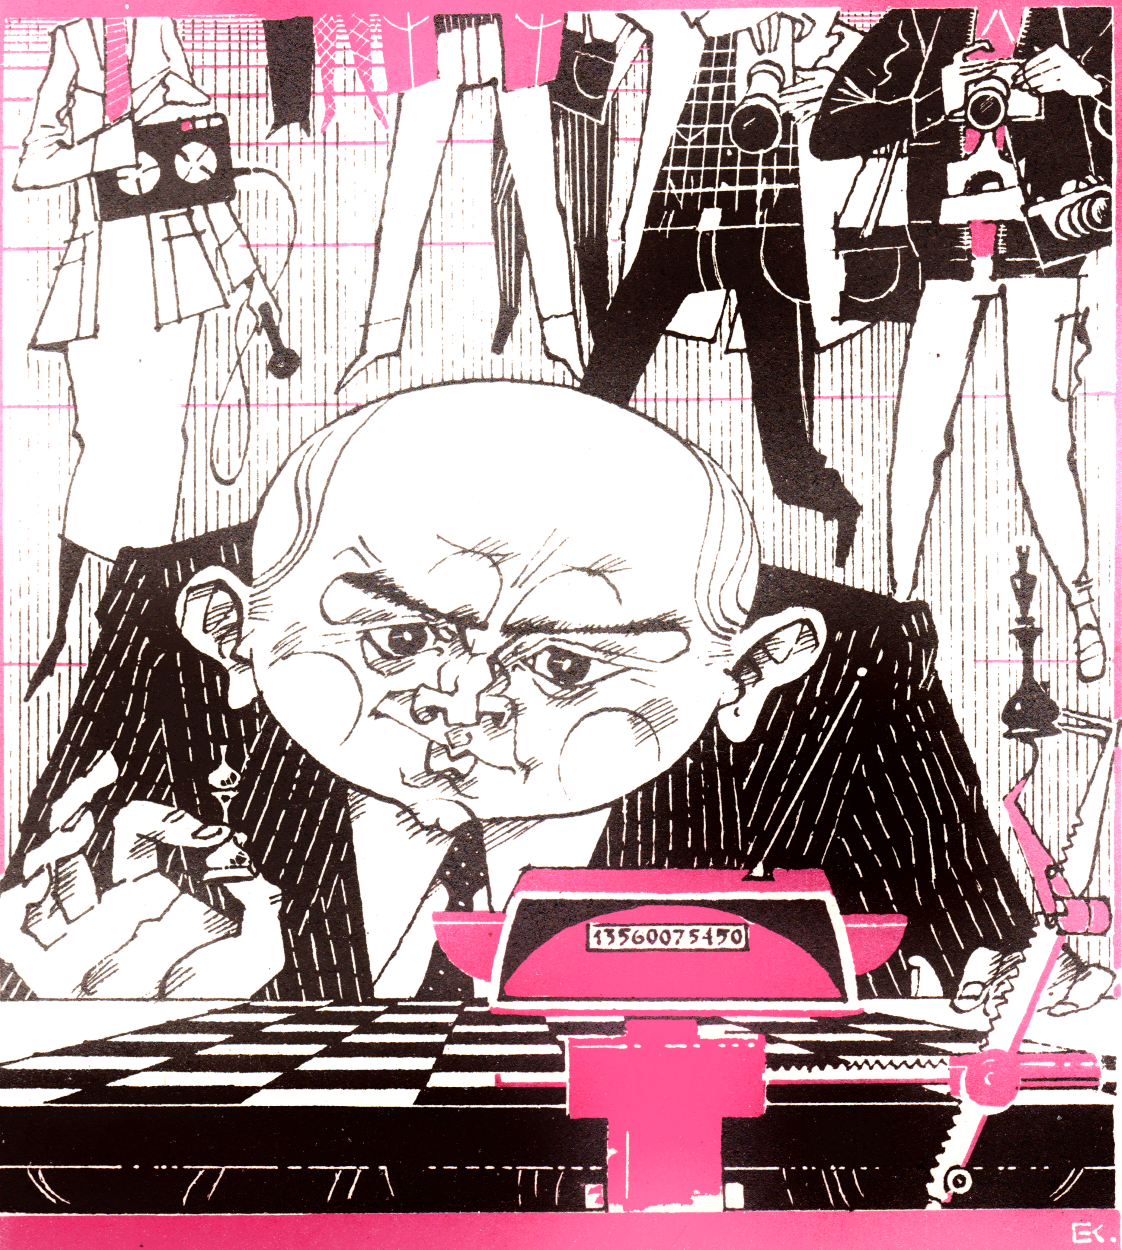
\includegraphics[width=\textwidth]{mail1}

«Уважаемая редакция. Недавно я узнал, что в журнале появился интересный раздел — Клуб электронных, игр. К сожалению, раньше я журнал не выписывал.

Предлагаю игру — поставить мат слоном и конем черному королю, которым играет ПМК «Электроника БЗ-34»:

00.В/О 01.3 02.ИП7 03.ИП4 04.— 05.Fx$^{2}$ 06.ИП8 07.ИП5 08.- 09.Fx$^{2}$
10.+ 11.- 12.Кх<оД 13.ИП4 14.ИП1 15.—	16.Fx$^{2}$ 17.ИП5 18.ИП2	19.—
20.Fx$^{2}$ 21.— 22.Кх$\neq$оД 23.ИП4 24.ИП0 25.— 26.Fx$^{2}$ 27.ИП5 28.ИПА 29.— 30.Fx$^{2}$ 31.+ 32.5 33.— 34.Кх$\neq$оД
35.ИП4 36.Кх$\neq$оД. 37.9 38.—
39.Кх$\neq$оД 40.ИП5 41.Кх$\neq$оД 42.9
43.— 44.Кх$\neq$оД 45.КИП3 46.ИП4 47.ИПД 48.$\div$ 49.ИП5 50.+ 51.С/П
52.ИП5 53.1 54.— 55.П5 56.КПП9
57.ИП4 58.1 59.— 60.П4 61.П6 62.КПП9 63.КИП4 64.КИП4 65.КПП9 66.ИПВ 67.ИПС 68./—/ 69.ПС 70.— 71.ПВ 72.КБПВ 73.КИП5 74.КПП9 75.ИП6 76.П4 77.КПП9 78.БП 79.89 80.ИП6 81.П4 82.КИП5 83.КПП9 84.КИП4
85.КИП4 86.КПП9 87.ИП6 88.П4
89.КИП5 90.КПП9 91.КИП4 92.КПП9 93.КИП4 94.КПП9 95.КИП3 96.ИП3 97.С/П

В регистры памяти записываются:

1 П9 73 ПВ 7 ПС 0,1 ПД. В регистрах П7, П8 записываются соответственно горизонтальная и вертикальная координаты белого короля, в регистрах П4, П5 — черного короля, в регистрах П1, П2 — слона, в регистрах ПО, ПА — коня. Для позиции на диаграмме записываем: 3 П7 5 П0 7 П1 1 П8 П2 ПА 5 П4 8 П5.

Фигуры можно расположить по-другому, слона надо ставить на черное поле. В регистр П3 записывается сигнал окончания игры Е50 (150 ВП 99 ВП П3). Перед началом игры надо перейти на адрес 52: БП 52.

Делаем первый ход, например Крс2. Записываем 2 П8, нажимаем клавишу С/П. Через 20 с на индикаторе появляется число 57 — ПМК показывает свой ход двузначным числом, первая цифра которого обозначает горизонтальную координату черного короля, вторая — вертикальную. Черные ответили Кре7.

В среднем ПМК «думает» над ходом около 50 с.

Записываем в регистры памяти новые координаты той фигуры, которой делаем ход, нажимаем С/П и т. д. Когда черному королю будет поставлен мат (или пат), на индикаторе появится символ Е с числом — количеством оставшихся до 50 ходов. Если появится другой символ (Г) с числом, это значит, что сделано больше 50 ходов и в соответствии с шахматными правилами игра считается закончившейся вничью.

Из-за ограниченных возможностей ПМК при игре надо соблюдать такие условия:
\begin{enumerate}
\item Ходы надо делать по правилам и не подставлять фигуры. ПМК не может проверить корректность хода и определить, можно ли «съесть» фигуру. (Коня при случае может и забрать.)
\item Мат надо поставить на поле h8 (88). Загнать черного короля на поле а1 очень легко, кроме того, ПМК можно поставить мат на. полях а8, h1 и других белых полях на краю доски, что при правильной игре черных сделать невозможно.
\item Надо учитывать, что ПМК считает битыми поля, которые простреливаются слоном через коня или короля. Например, в позиции: белые — Кра6, Ch2, Kg3, черные — Кра8 при ходе черных появится сигнал окончания игры.
\end{enumerate}

Хотя черные играют и не лучшим образом, начинающему шахматисту ПМК окажет упорное сопротивление.

В программе командами 52-94 задается порядок выбора ходов черного короля. Король стремится идти вперед, а если его не пускают, то командами 66-72 перебор полей поочередно меняется.

\begin{table}[H]
\begin{tabular}{|l|l|}
\hline
6 7 8 & 6 7 8 \\ \hline
4 5   & 5 4   \\ \hline
2 1 3 & 2 1 3 \\ \hline
\end{tabular}
\end{table}

(Цифрами указан порядок перебора полей, а король стоит в центре.)

Король «переставляется» на новое поле, и командой КПП9 происходит переход к подпрограмме. Командами 1-12 
проверяется, не попал ли король под удар белого короля, командами 13-22 — слона, 23-34 — коня. Командами 35-44 проверяется, не угодил ли король за пределы доски. Если на поле можно пойти, то командой 45 число ходов в регистре П3 уменьшается на единицу, командами 46—51 ход записывается в регистр X и счет останавливается. Если на поле пойти нельзя, то командой косвенного условного перехода управление передается на адрес 00, происходит возврат из подпрограммы и проверяется следующее поле. Когда у короля не останется свободных полей, на индикаторе появляется сигнал окончания игры.

После окончания игры стек подпрограмм остается заполненным, и перед набором другой программы, где переход на адрес 01 производится командой В/О, например космических игр, ПМК надо выключить. Кстати, если этот стек используется неполностью (практически так всегда и бывает), то, кроме адреса 01, командой В/О можно переходить и на адреса 12, 23, 34, 45, 56, 67, 78, 89, —0 (улавливаете закономерность?). Для этого перед набором основной программы надо заполнить стек подпрограмм числом, последняя цифра которого совпадает с первой цифрой указанных адресов, и очистить стек. Например, для перехода по адресу 45 нажимаем клавиши 4 П9 КБП9 FПРГ КПП9 ШГ влево F АВТ ПП ПП ПП ПП ПП В/О FПРГ В/О FABT В/О ПП В/О ПП В/О ПП В/О ПП В/О ПП. К сожалению, сохранение числа в стеке не предусмотрено. Теперь при каждой команде В/О вне подпрограмм управление передается на адрес 45.

Для перехода на адрес —0 стек заполняется числом 9 (или 19, 29, 39 и т. п.).

АВДЕЕВ Николай Андреевич,
радиоинженер. Поселок Сеймчан Магаданской области».

«Уважаемый Николай Андреевич! Спасибо за интересную программу. Шахматных у нас пока еще не встречалось, мы ее обязательно опубликуем. Но потребуется кое-какая доработка — внутренние резервы в игре есть. «Переключатель» вариантов перебора полей можно сделать попроще: 66. ИПС 67./—/ 68.ПС 69.Fx$\geq$0 70.80 71.КНОП 72.КНОП (адресация Ваша). Экономия — две команды и регистр В. Далее квадраты разностей координат черного короля и других фигур целесообразно находить с помощью ПП: 00.ИП5 01.— 02.Fx$^{2}$ 03.\XY 04.ИП4 05.— 06.Fx$^{2}$ 07.В/О (адреса условные), а перед обращением вызывать в нужном порядке координаты соответствующей белой фигуры, например, ИП7 ИП8 ПП и т. д. Это даст экономию еще в четыре команды. Если же использовать для вызова новой ПП освободившийся регистр В (обращение будет выглядеть, например, ИП7 ИП8 КППВ), освободятся еще три команды, всего девять, а это уже солидный резерв. В Вашем варианте не очень удобен ввод. Целесообразно, мне кажется, отвести регистры 1, 2 и 3 для хранения координат белых фигур в том виде, в котором Вы выводите координаты черного короля (например, el =51), сообщение Е50 в этом случае придется записать в регистр 0. Теперь при вводе (после С/П) достаточно вставить (адреса Ваши) 52.ПА 53.КПА, а ввод производить так: (номер фигуры) ПП (номер поля) С/П. В КППВ придется теперь еще и «расчленять» новые координаты на прежние. Она может, скажем, начинаться с фрагмента: 00.$\uparrow$ 01.ПА 02.ВП 03.— 04.FBx и далее: 05.ИП5 06.— 07.Fx$^{2}$ 08.\XY 09.ИПД 10.Х	11.ИП4 12.— 13.Fx$^{2}$ 14.В/О (адреса, как и прежде, условные). Такая процедура займет шесть команд из сэкономленных девяти (две при вводе плюс семь в ПП, зато на обращениях — они теперь имеют вид ИП1 КППВ — экономится три команды). Осталось три команды плюс два свободных регистра (7 и 8); с этим запасом, думаю, можно еще что-нибудь сообразить. Например, сделать так, чтобы черный король при случае мог «скушать» и белого слона. На это, видимо, нужно пять команд: сзади к КППВ пристыковывается +, слон проверяется последним, после обращения к измененной КППВ вставляется проверка на равенство нулю и отсылка на индикацию хода, затем FBx — FBx — и Ваша проверка (Кх$\neq$оД). Вставлено шесть команд, ушло две (команды + по Вашим адресам 10 и 31), итого, четыре. Три уже есть, а если, например, вставить перед КПП9 команды ИП6 П4 (на адреса 01 и 02), ввести в регистр 9 число 3, а в 8 — единицу, заменить фрагмент 75-77 на КПП8, фрагмент 80-83 на КИП5 КПП8, легко экономятся еще две команды. Возможно, есть и другие варианты улучшения качества игры (допустим, чтобы ПМК отличал поле 88, где он проигрывает, от других). В общем, посмотрите, что можно еще сделать. За информацию о стеке подпрограмм спасибо, такой у нас пока не было. Кстати, если при любом его заполнении сформировать ЗГГОГ (например, 1 ВП 50 Fx$^{2}$ Fx$^{2}$ Сх), то команда В/О (в программе) при первом исполнении передаст управление на 01, при втором — на 11, а затем — снова на 01. Этим приемом можно пользоваться при полном заполнении стека, чтобы не выключать ПМК при переходе к новой программе (или при каком-нибудь неприятном зацикливании).

С уважением, дежурный администратор КЭИ».

«Уважаемые товарищи!

Спасибо за рекомендации по улучшению программы. Способа, которым вы разделяете координаты, я не знал. (Далее следует измененный вариант программы.— М. П.) Изменено начало перебора полей черного короля: 1 2 3. Изменена проверка выхода короля за пределы доски.

Теперь условие, что нельзя подставлять фигуры, можно заменить другим — если черному королю удастся «съесть» одну из фигур, игра сразу считается ничьей (согласно «Шахматному кодексу» остался король с легкой фигурой против одинокого короля). После хода черных нажатием клавиши \XY можно узнать, сколько ходов еще можно сделать.

И все-таки, по-моему, проверка на «съедение» слона необязательна и лишь удлиняет время игры. Можно использовать этот резерв для улучшения игры черных. (Следует еще один вариант программы.— М. П.) В этом варианте черный король, попав на первую горизонталь (такое будет случаться часто), не будет топтаться на месте, сразу проверяется поле на пути к а1 и не тратится время на проверку невозможных ходов. Этот вариант мне нравится больше. Программу можно сократить еще на две команды, но этого слишком мало. Проверку на взятие слона можно ввести в программу для МК-61, у которого память побольше (у меня такого нет). Возможно, удастся еще вместить перебор полей только по первому варианту перебора при нахождении черного короля на восьмой горизонтали.

Отличать поле h8 от других калькулятору не нужно, это игру черных не улучшит. В таком окончании белые фигуры оттесняют черного короля в угол, цвет поля которого противоположен цвету полей, по которым ходит слон. (Идти в угол, где ставится мат, черные не хотят.) Затем черный король перегоняется в другой угол и получает мат. Из любого положения для мата требуется (теоретически) не более 36 ходов. Все надежды черного короля связаны с тем, что по дороге на эшафот ему удастся вырваться из-под конвоя белых фигур и белым придется начать все сначала. Вторично загнать черного короля в один угол, перевести его в другой и поставить мат белые обычно не успевают: согласно правилам, если за последние 50 ходов не было ходов пешками или взятий фигур или пешек, партия считается ничьей. Впрочем, иногда белые успевают перегнать короля по вертикали h и поставить мат. При измененном переборе полей все зависит от того, в какой момент короля выпустить.

Для начинающих это очень трудное окончание, многие даже уверены, что оно не выигрывается. Условие о поле h8 осложняет игру, зато отдельные слабые ходы ПМК облегчают задачу белых.

ПМК «думает» от 29 с до 2 мин 4 с. Но это зависит от конкретного экземпляра ПМК. Улучшить игру черных можно, если менять варианты перебора в зависимости от положения белых фигур или хотя бы одного короля. Однако такая программа в ПМК не помещается.

Н. А. АВДЕЕВ».

«Уважаемые товарищи!

16 августа я отправил ответ на ваше письмо и, видимо, поторопился. Два варианта программы легко объединяются в один. Вот он:

00.в/о 01.$\uparrow$ 02.ПА 03.ВП 04.- 05.FBx 06.ИП5 07.- 08.Fx$^{2}$ 09.\XY 10.ИПД 11.x 12.ИП4 13.- 14.Fx$^{2}$ 15.+ 16.в/о 17.ИП1 18.КППВ 19.3 20.- 21.Кх$\geq$оД 22.ИП3
23.КППВ 24.5 25.- 26.Кх$\neq$оД 27.ИП2 28.КППВ 29.Кх$\neq$о7 30.FBx 31.- 32.FBx 33.- 34.Кх$\neq$оД 35.ИП4 36.Кх$\neq$оД 37.9 38.- 39.Кх$\neq$оД 40.КИП0
41.ИП4 42.ИПД 43.$\div$ 44.ИП5 45.+ 46.с/п 47.ПА 48.КПА 49.ИП4 50.1 51.- 52.П4 53.П6 54.ИП5 55.1 56.- 57.Кх$\neq$о8 58.П5 59.КПП9 60.КИП4 61.КПП9 62.КИП4 63.КПП9 64.ИПС 65./-/ 66.ПС 67.Кх<оС 68.КИП5 69.ИП6 70.П4 71.КПП9 72.КИП4 73.КИП4 74.КПП9 75.ИП6 76.П4 77.БП 78.84 79.КИП5 80.КПП9 81.ИП6 82.П4 83.КПП9 84.КИП5 85.ИП5 86.9 87.- 88.Fx$\neq$0 89.95 90.КПП9 91.КИП4 92.КПП9 93.КИП4 94.КПП9 95.КИП0 96.ИП0 97.с/п

После перехода в режим АВТ нужно ввести в регистры следующие числа: 40 П7 71 П8 17 П9 1 ПВ 79 ПС 0,1 ПД, затем ввести в регистры 1, 2 и 3 начальные координаты белых фигур (короля, коня и слона; например, 31 П1 51 П2 71 ПЗ), в регистры 4 и 5 горизонтальную и вертикальную координаты черного короля (скажем, 5 П4 8 П5), в регистр 0 — сообщение Е50, перед началом игры скомандовать БП 47 и делать первый ход: (номер фигуры) ПП (номер поля) С/П. Какое-то время ПМК «думает», затем выводит на индикатор новые координаты своего короля и уступает очередь хода сопернику. Желаю многих побед!

С уважением, АВДЕЕВ Н. А.

19 августа 1986».

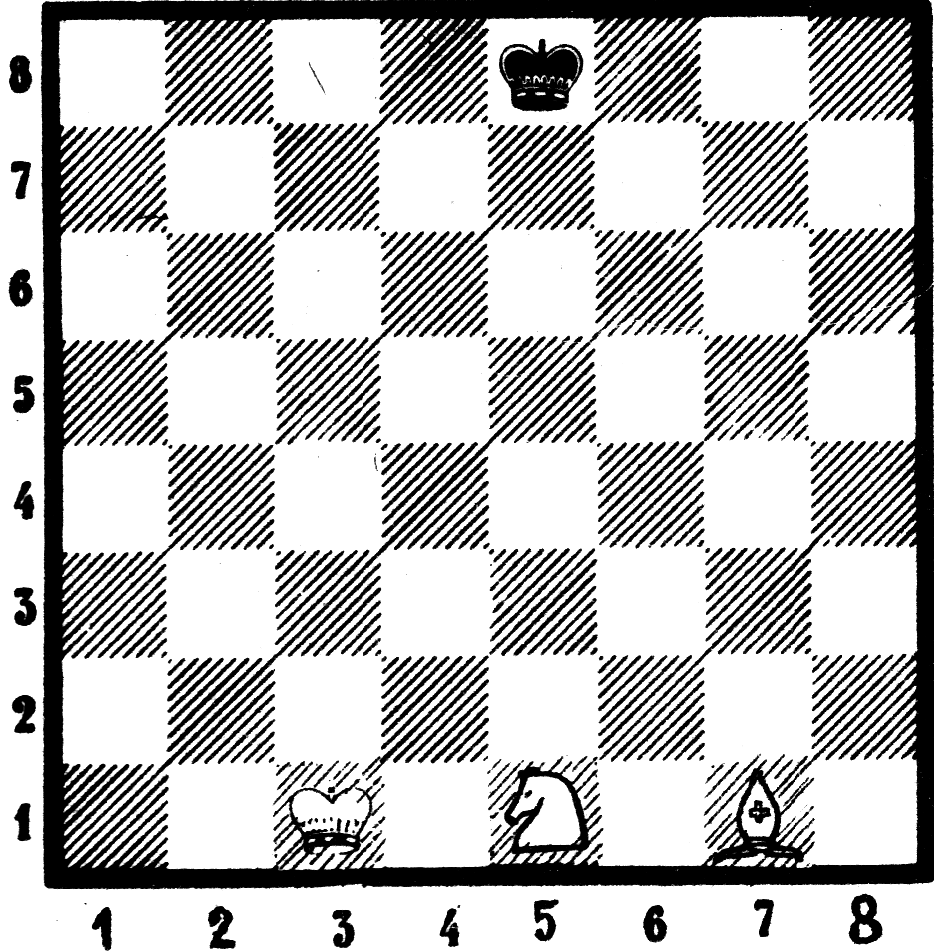
\includegraphics[width=\textwidth]{mail2}

Итак, первая шахматная программа для ПМК... А ведь всего четыре месяца назад (в № 8) одна лишь робкая мысль о чем-то подобном вызвала появление на наших страницах выражений вроде: «Не вполне обоснованная вера во всемогущество ПМК», «Какие там шахматы!», «Пиши пропало, ходи как попало» и т. д. Время, как видим, убедительно показало правоту читателя В. Ревуцкого из Киева, обратившегося в редакцию с просьбой публиковать такие программы.

Надеемся, что предание гласности нашей переписки с Н. Авдеевым поможет читателям, разрабатывающим собственные игровые программы. Кстати, когда номер уже был в производстве, аналогичную игру (мат конем и слоном) прислал и ветеран эпопеи «Кон-Тики» Л. Роканиди из Сызрани. Со своей стороны, администрация КЭИ решила тряхнуть стариной, извлекла из заржавленных пороховниц кое-какие нестандартные приемы и разразилась следующим вариантом:

00.ИП3 01.$\div$ 02.КИП3 03.ИП5 04.ИП1 05.- 06.$\div$ 07.* 08.с/п 09.П7 10.КП7 11.КИП1 12.КППБ 13.КППА 44.КППВ 15.1 46.КППС 17.ИП8 18.2 19.x 20./-/ 21.КППС 22.1 23.КППС 24.КППВ 25.КППВ 26.КИП1
27.КППА 28.ИП9 29.ИП8 30./-/ 31.П8 32.ИП8 33.ИП1 34.+ 35.$\uparrow$ 36.П1 37.ВП 38.П2 39.Кх$\neq$о9 40.9 41.- 42.Кх$\neq$o9 43.ИП1 44.Кх$\neq$о9 45.Fcos
46.Кх$\geq$о9 47.ИП4 48.КППД 49.+ 50.Кх$\neq$о0 51.3 52.- 53.Кх$\neq$о9 54.ИП5 55.КППД 56.+ 57.5 58.- 59.Кх$\neq$о9 60.ИП6 61.КППД 62.F$\sqrt{}$ 63.П2 64.* 65.- 66.Кх=оЕ 67.ИП7 68.+ 69.П7 70.ИП4 71.- 72.Кх$\neq$оЕ 73.ИП7 74.ИП5 75.- 76.Кх$\neq$оЕ 77.ИП1 78.ИП7 79.- 80.ИП2 81.$\div$ 82.FL2 83.67 84.П7 85.ВП 86.ИП2 87.- 88.Fx$^{2}$ 89.FBx 90.ИП7 91.- 92.ИП1 93.+ 94.ИП8 95.$\div$ 96.Fx$^{2}$ 97.в/о

По адресам 07 и 64 стоит десятичная точка, букве Е в командах по адресам 66, 72 и 76 на клавиатуре Б3-34 соответствует стрелка вверх. В буквенные регистры вводятся адреса переходов: 29 ПА 32 ПВ 33 ПС 84 ПД. В регистр 9 вводится слово ЗГГОГ, являющееся одновременно адресом перехода 97: 1 ВП 50 Fx$^{2}$ Fx$^{2}$ 97 Х П9 (кстати сказать, к абсолютно такой же идее «совмещения функций» пришел и десятиклассник С. Ишутин из Свердловска в своей модификации программы «Козлик и волки»), В регистры 3 и 8 вводятся константы: 50 П3 10 /—/ П8. (Содержание регистра 3 — это число ходов, отпущенных на игру; если вы в себе уверены, можете ввестй сюда 30 или, допустим, 20). Регистр 0 зануляется: 0 П0. (Так должны поступить владельцы БЗ-34 и МК-54; обладатели МК-61 и МК-52 должны еще и задействовать регистр Е: 0 ПЕ 2 П0.) Наконец в регистре 1 располагается координата черного короля (скажем, 58 П1), в регистрах 4, 5 и 6 — соответственно координаты белого короля, коня и слона (допустим, 31 П4 51 П5 71 П6). Слона можно ставить как на белое, так и на черное поле; мат полагается делать только на восьмой горизонтали.

Перед началом новой игры, кроме координат фигур, нужно заново вводить содержимое регистров 0, 3 и 8. Переключатель Р—Г устанавливается в положение Г. Игра начинается командой В/О С/П. При останове на индикаторе светится текущая координата черного короля. Ход белых задается стандартно: (номер фигуры) ПП (номер поля) С/П (не забывайте, что в отличие от предыдущей программы фигурам белых соответствуют номера 4, 5 и 6).

Данная программа отличается от программы Н. Авдеева несколько более глубокими знаниями правил. При исчерпании лимита ходов высвечивается сообщение ЕГГОГ; тот же сигнал появляется и когда черный король «поедает» незащищенного слона либо коня белых или же когда белый король приближается к нему вплотную, нарушив тем самым правила (правда, в каждом из этих случаев черные могут и в свою очередь «зевнуть», уйдя на свободное поле). Программа пропускает черного короля на поля, находящиеся на той же диагонали, что и слон, но «заэкранированные» белым конем либо королем. ПМК отличает мат от пата: в первом случае на индикаторе загорается сообщение ЗГГОГ, во втором высвечиваются прежние координаты черного короля. ЗГГОГ появляется на экранчике и за 9 ходов до исчерпания выделенного лимита ходов, предупреждая, что времени осталось в обрез. В этом случае надо скомандовать В/О С/П и продолжать игру. Чтобы такое предупреждение не выдавалось, нужно заменить первые три команды: 00.FL3 01.03 02.К— (вариант предложен В. Алексеевым). Теперь, как обычно, совершим краткую прогулку по программе.

Команды 00—02 проверяют (в обоих вариантах), не исчерпан ли лимит оставшихся ходов, и уменьшают его на единичку. Если исчерпан, на экране появляется ЕГГОГ (из-за деления по адресу 01 либо в результате некорректной операции К—). Если же содержимое регистра 3 перед входом в блок равно десяти, то в основном варианте команда КИПЗ эквивалентна ИП9 и на экране появляется ЗГГОГ, сидящий в регистре 9. Команды 03-06 проверяют, не «скушал» ли ненароком черный король белого коня: если координаты совпадают, на индикаторе появляется ЕГГОГ. Команда по адресу 07 (ее код 0—) не встречалась пока в наших программах. Она вызывает на индикатор последний из результатов вызова из памяти, FBx, F$\pi^{2}$, ввода в стек записанной в программе константы, команд переходов и подпрограммы, оставляя содержимое регистра У неизменным. К сожалению (к этому мы уже успели привыкнуть) , и это полезное свойство осталось неосвещенным на страницах заводской инструкции.

В данном случае команда «точка» эквивалентна ИП1 и ни к какой экономии не приводит. Зато легче будет понять работу этой команды, записанной по адресу 64. Пойдем дальше. Команда С/П останавливает ПМК для индикации координат черного короля. Команды ввода 09—10 записывают заданный номер фигуры (допустим, 4) в регистр 7 и вносят новую координату в соответствующий регистр (в нашем случае 4). Команды 11—27 осуществляют перебор вариантов хода черного короля по одной из двух схем:
\begin{table}[H]
\begin{tabular}{|l|l|}
\hline
6 7 8 & 8 7 6 \\ \hline
5 9 4 & 4 9 5 \\ \hline
1 2 3 & 3 2 1 \\ \hline
\end{tabular}
\end{table}
— которые меняются ход от хода. Последним, как видим, проверяется исходное поле, на котором стоит король. Если и этот ход невозможен (поле под боем), команда по адресу 28 вызывает на индикатор сообщение ЗГГОГ: ходить некуда, мат.

При переборе полей используется основная подпрограмма, расположенная на адресах 29-83. Начальных адресов у нее три: 29 (КППА), 32 (КППВ), 33 (КППС); то или иное обращение используется в зависимости от ситуации. К основной подпрограмме сзади «пристыкована» подпрограмма КППД (84-97); в программе не хватило места, чтобы поставить после адреса 83 команду В/О. Действие подпрограммы рассмотрим на примере первого обращения (11-12).

Команда КИП1 (11) переносит черного короля на следующую горизонталь: например, с 8-й на 7-ю. Команда КППВ (12) эквивалентна ПП 32. Первая команда подпрограммы вызывает содержимое регистра 8, а его знак меняется ход от хода. Допустим, там —10; это число складывается с новым содержимым регистра 1 — король пошел «вниз-влево». Блок 35—38 заносит новую координату короля, в регистр 1, «срезает» первую цифру (нестандартно используется команда ВП), а вторую заносит в регистр 2. Равенство последней нулю соответствует выходу короля за нижнюю либо левую границу доски (кроме поля 00 — оно проверяется особо). Если такое случилось, команда перехода (39) передает управление на В/О (97), а та возвращает его на адрес 13, и начинается проверка очередного хода. Если же все в порядке, фрагмент 40—42 проверяет выход за верхнюю границу доски, 43—44 — на фиктивное «поле» 00, 45—46 — за правую границу. Если все в порядке, наступает очередь проверок битых полей.

Первой «к барьеру» вызывается координата белого короля (47). Тут же следует обращение КППД — к вспомогательной подпрограмме (84—97), после возврата из которой в регистре У оказывается квадрат разности вертикальных координат черного и белого королей, в регистре X — то же для горизонтальных координат. Эти величины суммируются (49); если сумма равна нулю (совпадение координат), значит, белые ошиблись, на своем ходе вплотную придвинув своего короля к королю противника. Команда 50 модифицирует содержимое регистра 0 (там был ноль) в —99999999, и управление передается на последние две цифры числа: адрес 99 короткой побочной ветви (при игре с Б3-34). Исполняется дубль-команда $\div$ (адрес 01), на индикаторе выскакивает ЕГГОГ. При игре с МК-61 происходит модификация 2 в 1 с теми же последствиями.

Если проверка завершилась успешно, из полученной суммы вычитается тройка; если результат отрицателен, ход запрещен — короли сближаются вплотную (51—53).

Затем наступает очередь коня (54-59). Из суммы квадратов разностей вертикальных и горизонтальных координат вычитается 5 — легко видеть, что «ход конем» соответствует именно этому значению.

Проверка слона (60-83) начинается по той же схеме (60-61). Команды 62-64 заносят в регистр 2 модуль разности горизонтальных координат слона и черного короля, затем восстанавливают стек. Далее следует проверка того, не стоит ли король на одной из простреливаемых слоном диагоналей (65-66). Если нет, то такой ход возможен (все проверки закончены) и управление передается на адрес 00 для индикации новых координат черного короля. В противном случае циклом 67-83 проверяются все поля, разделяющие черного короля и слона: не стоит ли на одном из них король или конь белых? Если да, ход опять-таки допустим, управление передается на адрес 00. При совпадении координат слона и черного короля (слон «съеден») содержимое регистра 2 еще до входа в цикл равно нулю и команды 80-81 выводят на индикатор ЕГГОГ. Если же диагональ полностью свободна, цикл заканчивается, затем «вхолостую» отрабатывает КППД (84—97), ход невозможен, и ПМК начинает обдумывать следующий. И все повторяется.

\subsection{ПОЗДРАВЛЯЕМ ПОБЕДИТЕЛЕЙ}

Подведены итоги первого в истории космонавтики массового перелета по маршруту Луна — Земля на электронных лунолетах системы «Кон-Тики». Победителями признаны следующие участники астропробега:
\begin{enumerate}
\item Александр АРТАМОНОВ (г. Апрелевка Московской области).
\item Александр АУЛА (г. 3апорожье).
\item Андрей ДОЛГАЛЛО (г. Ленинград).
\item Анатолий КОЛОСОВ (с. Пышуг Костромской области).
\item Юрий КУЗНЕЦОВ (г. Куйбышев)
\item Вадим ЛАДОХИН (г. Сургут Тюменской области).
\item Лев РОКАНИДИ (г. Сызрань).
\item Сергей СВИНОЛОБОВ (г. Днепропетровск).
\item Павел ТРУБАЕВ (г. Белгород).
\item Валерий ШИЛОВ (г. Ярославль).
\end{enumerate}

Все они награждены дипломами имени Юрия Гагарина, с чем мы их от всей души поздравляем.

Многие читатели в своих письмах высказывают справедливый упрек: КЭИ в своих публикациях игнорирует расширенные возможности новых моделей ПМК — МК-61 и МК-52. Действительно, наличие семи лишних команд и одного дополнительного регистра позволяет, например, легко добиться того, чтобы ПМК в патовой ситуации выдавал на индикатор ЕГГОГ. Для этого достаточно между командами 07-08 вставить фрагмент: 08.ИП0 09.— 10.$\div$ 11.ИП1 12.П0, команду по старому адресу 50. Кх$\neq$о0 заменить двумя Fx$\neq$o 01, в конце основной подпрограммы (после старого адреса 83) поставить В/О. Вот и все изменения, не считая того, что из-за сдвига адресов перед игрой вводится другой комплект исходных данных: 34 ПА 37 ПВ 38 ПС 0 ПЕ П0 91 ПД 1 ВП 50 Fx$^{2}$ Fx$^{2}$ 90 X П9 50 П3 10 /—/ П8. А для утешения владельцев Б3-34 и МК-54 сообщаем, что на их ПМК можно в любой момент игры передать очередь хода черным: Сх С/П.

В заключение администрация КЭИ объявляет Николаю Авдееву благодарность и выражает надежду, что предложенные идеи помогут читателям в разработке собственных шахматных игр: мат ферзем, ладьей, двумя слонами и даже (да простят нас профессионалы) двумя конями!

Михаил ПУХОВ

С Новым годом!

\section{ВЕК НАЧНЕТСЯ С ПОНЕДЕЛЬНИКА}

\end{document}
